\documentclass[twoside]{book}

% Packages required by doxygen
\usepackage{fixltx2e}
\usepackage{calc}
\usepackage{doxygen}
\usepackage[export]{adjustbox} % also loads graphicx
\usepackage{graphicx}
\usepackage[utf8]{inputenc}
\usepackage{makeidx}
\usepackage{multicol}
\usepackage{multirow}
\PassOptionsToPackage{warn}{textcomp}
\usepackage{textcomp}
\usepackage[nointegrals]{wasysym}
\usepackage[table]{xcolor}

% Font selection
\usepackage[T1]{fontenc}
\usepackage[scaled=.90]{helvet}
\usepackage{courier}
\usepackage{amssymb}
\usepackage{sectsty}
\renewcommand{\familydefault}{\sfdefault}
\allsectionsfont{%
  \fontseries{bc}\selectfont%
  \color{darkgray}%
}
\renewcommand{\DoxyLabelFont}{%
  \fontseries{bc}\selectfont%
  \color{darkgray}%
}
\newcommand{\+}{\discretionary{\mbox{\scriptsize$\hookleftarrow$}}{}{}}

% Page & text layout
\usepackage{geometry}
\geometry{%
  a4paper,%
  top=2.5cm,%
  bottom=2.5cm,%
  left=2.5cm,%
  right=2.5cm%
}
\tolerance=750
\hfuzz=15pt
\hbadness=750
\setlength{\emergencystretch}{15pt}
\setlength{\parindent}{0cm}
\setlength{\parskip}{3ex plus 2ex minus 2ex}
\makeatletter
\renewcommand{\paragraph}{%
  \@startsection{paragraph}{4}{0ex}{-1.0ex}{1.0ex}{%
    \normalfont\normalsize\bfseries\SS@parafont%
  }%
}
\renewcommand{\subparagraph}{%
  \@startsection{subparagraph}{5}{0ex}{-1.0ex}{1.0ex}{%
    \normalfont\normalsize\bfseries\SS@subparafont%
  }%
}
\makeatother

% Headers & footers
\usepackage{fancyhdr}
\pagestyle{fancyplain}
\fancyhead[LE]{\fancyplain{}{\bfseries\thepage}}
\fancyhead[CE]{\fancyplain{}{}}
\fancyhead[RE]{\fancyplain{}{\bfseries\leftmark}}
\fancyhead[LO]{\fancyplain{}{\bfseries\rightmark}}
\fancyhead[CO]{\fancyplain{}{}}
\fancyhead[RO]{\fancyplain{}{\bfseries\thepage}}
\fancyfoot[LE]{\fancyplain{}{}}
\fancyfoot[CE]{\fancyplain{}{}}
\fancyfoot[RE]{\fancyplain{}{\bfseries\scriptsize Generated by Doxygen }}
\fancyfoot[LO]{\fancyplain{}{\bfseries\scriptsize Generated by Doxygen }}
\fancyfoot[CO]{\fancyplain{}{}}
\fancyfoot[RO]{\fancyplain{}{}}
\renewcommand{\footrulewidth}{0.4pt}
\renewcommand{\chaptermark}[1]{%
  \markboth{#1}{}%
}
\renewcommand{\sectionmark}[1]{%
  \markright{\thesection\ #1}%
}

% Indices & bibliography
\usepackage{natbib}
\usepackage[titles]{tocloft}
\setcounter{tocdepth}{3}
\setcounter{secnumdepth}{5}
\makeindex

% Hyperlinks (required, but should be loaded last)
\usepackage{ifpdf}
\ifpdf
  \usepackage[pdftex,pagebackref=true]{hyperref}
\else
  \usepackage[ps2pdf,pagebackref=true]{hyperref}
\fi
\hypersetup{%
  colorlinks=true,%
  linkcolor=blue,%
  citecolor=blue,%
  unicode%
}

% Custom commands
\newcommand{\clearemptydoublepage}{%
  \newpage{\pagestyle{empty}\cleardoublepage}%
}

\usepackage{caption}
\captionsetup{labelsep=space,justification=centering,font={bf},singlelinecheck=off,skip=4pt,position=top}

%===== C O N T E N T S =====

\begin{document}

% Titlepage & ToC
\hypersetup{pageanchor=false,
             bookmarksnumbered=true,
             pdfencoding=unicode
            }
\pagenumbering{alph}
\begin{titlepage}
\vspace*{7cm}
\begin{center}%
{\Large My Project }\\
\vspace*{1cm}
{\large Generated by Doxygen 1.8.12}\\
\end{center}
\end{titlepage}
\clearemptydoublepage
\pagenumbering{roman}
\tableofcontents
\clearemptydoublepage
\pagenumbering{arabic}
\hypersetup{pageanchor=true}

%--- Begin generated contents ---
\chapter{Hierarchical Index}
\section{Class Hierarchy}
This inheritance list is sorted roughly, but not completely, alphabetically\+:\begin{DoxyCompactList}
\item \contentsline{section}{Bootstrap$<$ T, U $>$}{\pageref{classBootstrap}}{}
\item \contentsline{section}{Compute\+Return}{\pageref{classComputeReturn}}{}
\item \contentsline{section}{copula\+Rng}{\pageref{classcopulaRng}}{}
\item \contentsline{section}{Gen\+From\+Distr$<$ T $>$}{\pageref{classGenFromDistr}}{}
\item \contentsline{section}{Instrument}{\pageref{classInstrument}}{}
\begin{DoxyCompactList}
\item \contentsline{section}{Delta\+One}{\pageref{classDeltaOne}}{}
\item \contentsline{section}{Derivatives}{\pageref{classDerivatives}}{}
\item \contentsline{section}{Equity}{\pageref{classEquity}}{}
\item \contentsline{section}{FI}{\pageref{classFI}}{}
\end{DoxyCompactList}
\item \contentsline{section}{M\+C\+Engine$<$ T, U $>$}{\pageref{classMCEngine}}{}
\begin{DoxyCompactList}
\item \contentsline{section}{Copula\+Engine$<$ T, U $>$}{\pageref{classCopulaEngine}}{}
\end{DoxyCompactList}
\item \contentsline{section}{Path}{\pageref{classPath}}{}
\begin{DoxyCompactList}
\item \contentsline{section}{A\+R1x\+G\+A\+R\+C\+H11}{\pageref{classAR1xGARCH11}}{}
\item \contentsline{section}{G\+A\+R\+C\+H11}{\pageref{classGARCH11}}{}
\item \contentsline{section}{Path1x1}{\pageref{classPath1x1}}{}
\end{DoxyCompactList}
\item \contentsline{section}{Pca}{\pageref{classPca}}{}
\item \contentsline{section}{Portfolio}{\pageref{classPortfolio}}{}
\item \contentsline{section}{rng}{\pageref{classrng}}{}
\item \contentsline{section}{VaR}{\pageref{classVaR}}{}
\begin{DoxyCompactList}
\item \contentsline{section}{Extreme\+Value\+VaR}{\pageref{classExtremeValueVaR}}{}
\begin{DoxyCompactList}
\item \contentsline{section}{Po\+T\+VaR}{\pageref{classPoTVaR}}{}
\end{DoxyCompactList}
\item \contentsline{section}{None\+Parametric\+VaR}{\pageref{classNoneParametricVaR}}{}
\begin{DoxyCompactList}
\item \contentsline{section}{Historical\+VaR}{\pageref{classHistoricalVaR}}{}
\end{DoxyCompactList}
\item \contentsline{section}{Parametric\+VaR}{\pageref{classParametricVaR}}{}
\begin{DoxyCompactList}
\item \contentsline{section}{Garch\+VaR}{\pageref{classGarchVaR}}{}
\item \contentsline{section}{Risk\+Metrics\+VaR}{\pageref{classRiskMetricsVaR}}{}
\end{DoxyCompactList}
\end{DoxyCompactList}
\item \contentsline{section}{Va\+R\+Bridge}{\pageref{classVaRBridge}}{}
\item \contentsline{section}{Va\+R\+Compute$<$ T, U $>$}{\pageref{classVaRCompute}}{}
\begin{DoxyCompactList}
\item \contentsline{section}{Va\+R\+Copula\+Compute$<$ T, U, V $>$}{\pageref{classVaRCopulaCompute}}{}
\item \contentsline{section}{Va\+R\+Extreme\+Value\+Compute$<$ T, U $>$}{\pageref{classVaRExtremeValueCompute}}{}
\item \contentsline{section}{Va\+R\+Monte\+Carlo\+Compute$<$ T, U, V $>$}{\pageref{classVaRMonteCarloCompute}}{}
\item \contentsline{section}{Va\+Rnone\+Param\+Compute$<$ T, U $>$}{\pageref{classVaRnoneParamCompute}}{}
\item \contentsline{section}{Va\+R\+Param\+Compute$<$ T, U $>$}{\pageref{classVaRParamCompute}}{}
\end{DoxyCompactList}
\item \contentsline{section}{Va\+R\+Ptf\+Compute}{\pageref{classVaRPtfCompute}}{}
\begin{DoxyCompactList}
\item \contentsline{section}{Va\+R\+Ptf\+M\+C\+Compute$<$ T, V $>$}{\pageref{classVaRPtfMCCompute}}{}
\end{DoxyCompactList}
\end{DoxyCompactList}

\chapter{Class Index}
\section{Class List}
Here are the classes, structs, unions and interfaces with brief descriptions\+:\begin{DoxyCompactList}
\item\contentsline{section}{\hyperlink{classAR1xGARCH11}{A\+R1x\+G\+A\+R\+C\+H11} \\*Model A\+R(1) x G\+A\+R\+C\+H(1,1) -\/ Fat tails }{\pageref{classAR1xGARCH11}}{}
\item\contentsline{section}{\hyperlink{classBootstrap}{Bootstrap$<$ T, U $>$} }{\pageref{classBootstrap}}{}
\item\contentsline{section}{\hyperlink{classComputeReturn}{Compute\+Return} }{\pageref{classComputeReturn}}{}
\item\contentsline{section}{\hyperlink{classCopulaEngine}{Copula\+Engine$<$ T, U $>$} \\*T rng, U path }{\pageref{classCopulaEngine}}{}
\item\contentsline{section}{\hyperlink{classcopulaRng}{copula\+Rng} }{\pageref{classcopulaRng}}{}
\item\contentsline{section}{\hyperlink{classDeltaOne}{Delta\+One} \\*Sensitivity one for one. FX, index, commodity prices }{\pageref{classDeltaOne}}{}
\item\contentsline{section}{\hyperlink{classDerivatives}{Derivatives} }{\pageref{classDerivatives}}{}
\item\contentsline{section}{\hyperlink{classEquity}{Equity} }{\pageref{classEquity}}{}
\item\contentsline{section}{\hyperlink{classExtremeValueVaR}{Extreme\+Value\+VaR} }{\pageref{classExtremeValueVaR}}{}
\item\contentsline{section}{\hyperlink{classFI}{FI} }{\pageref{classFI}}{}
\item\contentsline{section}{\hyperlink{classGARCH11}{G\+A\+R\+C\+H11} \\*Model G\+A\+R\+C\+H(1,1) }{\pageref{classGARCH11}}{}
\item\contentsline{section}{\hyperlink{classGarchVaR}{Garch\+VaR} \\*Compute G\+A\+R\+C\+H(1,1) \hyperlink{classVaR}{VaR} }{\pageref{classGarchVaR}}{}
\item\contentsline{section}{\hyperlink{classGenFromDistr}{Gen\+From\+Distr$<$ T $>$} \\*Generate random number according to specified distribution }{\pageref{classGenFromDistr}}{}
\item\contentsline{section}{\hyperlink{classHistoricalVaR}{Historical\+VaR} \\*Compute \hyperlink{classVaR}{VaR} using historical method (histogram method) }{\pageref{classHistoricalVaR}}{}
\item\contentsline{section}{\hyperlink{classInstrument}{Instrument} }{\pageref{classInstrument}}{}
\item\contentsline{section}{\hyperlink{classMCEngine}{M\+C\+Engine$<$ T, U $>$} \\*Student\textquotesingle{}s t-\/distr }{\pageref{classMCEngine}}{}
\item\contentsline{section}{\hyperlink{classNoneParametricVaR}{None\+Parametric\+VaR} }{\pageref{classNoneParametricVaR}}{}
\item\contentsline{section}{\hyperlink{classParametricVaR}{Parametric\+VaR} }{\pageref{classParametricVaR}}{}
\item\contentsline{section}{\hyperlink{classPath}{Path} \\*\hyperlink{classPath}{Path} fait tail, mean-\/reverting, commodity process .. }{\pageref{classPath}}{}
\item\contentsline{section}{\hyperlink{classPath1x1}{Path1x1} }{\pageref{classPath1x1}}{}
\item\contentsline{section}{\hyperlink{classPca}{Pca} }{\pageref{classPca}}{}
\item\contentsline{section}{\hyperlink{classPortfolio}{Portfolio} }{\pageref{classPortfolio}}{}
\item\contentsline{section}{\hyperlink{classPoTVaR}{Po\+T\+VaR} }{\pageref{classPoTVaR}}{}
\item\contentsline{section}{\hyperlink{classRiskMetricsVaR}{Risk\+Metrics\+VaR} \\*Compute Risk metrics \hyperlink{classVaR}{VaR} aka Exponential Weight Moving Average (E\+W\+MA) }{\pageref{classRiskMetricsVaR}}{}
\item\contentsline{section}{\hyperlink{classrng}{rng} \\*Mersenne-\/\+Twister pseudo random number generator }{\pageref{classrng}}{}
\item\contentsline{section}{\hyperlink{classVaR}{VaR} }{\pageref{classVaR}}{}
\item\contentsline{section}{\hyperlink{classVaRBridge}{Va\+R\+Bridge} }{\pageref{classVaRBridge}}{}
\item\contentsline{section}{\hyperlink{classVaRCompute}{Va\+R\+Compute$<$ T, U $>$} \\*Compute \hyperlink{classVaR}{VaR} }{\pageref{classVaRCompute}}{}
\item\contentsline{section}{\hyperlink{classVaRCopulaCompute}{Va\+R\+Copula\+Compute$<$ T, U, V $>$} \\*Compute \hyperlink{classVaR}{VaR} using Monte Carlo \& Copula }{\pageref{classVaRCopulaCompute}}{}
\item\contentsline{section}{\hyperlink{classVaRExtremeValueCompute}{Va\+R\+Extreme\+Value\+Compute$<$ T, U $>$} \\*Compute \hyperlink{classVaR}{VaR} using extreme value -\/ Generalized Pareto }{\pageref{classVaRExtremeValueCompute}}{}
\item\contentsline{section}{\hyperlink{classVaRMonteCarloCompute}{Va\+R\+Monte\+Carlo\+Compute$<$ T, U, V $>$} \\*Compute \hyperlink{classVaR}{VaR} using Monte Carlo }{\pageref{classVaRMonteCarloCompute}}{}
\item\contentsline{section}{\hyperlink{classVaRnoneParamCompute}{Va\+Rnone\+Param\+Compute$<$ T, U $>$} \\*Compute \hyperlink{classVaR}{VaR} using none-\/parametric model }{\pageref{classVaRnoneParamCompute}}{}
\item\contentsline{section}{\hyperlink{classVaRParamCompute}{Va\+R\+Param\+Compute$<$ T, U $>$} \\*Compute \hyperlink{classVaR}{VaR} using parametric mode }{\pageref{classVaRParamCompute}}{}
\item\contentsline{section}{\hyperlink{classVaRPtfCompute}{Va\+R\+Ptf\+Compute} \\*Compute ptf\textquotesingle{}s \hyperlink{classVaR}{VaR} using parametric approach }{\pageref{classVaRPtfCompute}}{}
\item\contentsline{section}{\hyperlink{classVaRPtfMCCompute}{Va\+R\+Ptf\+M\+C\+Compute$<$ T, V $>$} \\*Compute \hyperlink{classVaR}{VaR} of a portfolio through Monte Carlo simulation }{\pageref{classVaRPtfMCCompute}}{}
\end{DoxyCompactList}

\chapter{File Index}
\section{File List}
Here is a list of all files with brief descriptions\+:\begin{DoxyCompactList}
\item\contentsline{section}{\hyperlink{bootstrap_8h}{bootstrap.\+h} }{\pageref{bootstrap_8h}}{}
\item\contentsline{section}{\hyperlink{compute__returns__eigen_8h}{compute\+\_\+returns\+\_\+eigen.\+h} }{\pageref{compute__returns__eigen_8h}}{}
\item\contentsline{section}{\hyperlink{compute__var_8h}{compute\+\_\+var.\+h} }{\pageref{compute__var_8h}}{}
\item\contentsline{section}{\hyperlink{generate__rm__from__distr_8h}{generate\+\_\+rm\+\_\+from\+\_\+distr.\+h} }{\pageref{generate__rm__from__distr_8h}}{}
\item\contentsline{section}{\hyperlink{instrument_8h}{instrument.\+h} }{\pageref{instrument_8h}}{}
\item\contentsline{section}{\hyperlink{mc__engine_8h}{mc\+\_\+engine.\+h} }{\pageref{mc__engine_8h}}{}
\item\contentsline{section}{\hyperlink{path_8h}{path.\+h} }{\pageref{path_8h}}{}
\item\contentsline{section}{\hyperlink{pca_8h}{pca.\+h} }{\pageref{pca_8h}}{}
\item\contentsline{section}{\hyperlink{portfolio_8h}{portfolio.\+h} }{\pageref{portfolio_8h}}{}
\item\contentsline{section}{\hyperlink{ptf__var_8h}{ptf\+\_\+var.\+h} }{\pageref{ptf__var_8h}}{}
\item\contentsline{section}{\hyperlink{rng_8h}{rng.\+h} }{\pageref{rng_8h}}{}
\item\contentsline{section}{\hyperlink{var__bridge_8h}{var\+\_\+bridge.\+h} }{\pageref{var__bridge_8h}}{}
\item\contentsline{section}{\hyperlink{var__model_8h}{var\+\_\+model.\+h} }{\pageref{var__model_8h}}{}
\end{DoxyCompactList}

\chapter{Class Documentation}
\hypertarget{classAR1xGARCH11}{}\section{A\+R1x\+G\+A\+R\+C\+H11 Class Reference}
\label{classAR1xGARCH11}\index{A\+R1x\+G\+A\+R\+C\+H11@{A\+R1x\+G\+A\+R\+C\+H11}}


model A\+R(1) x G\+A\+R\+C\+H(1,1) -\/ Fat tails  




{\ttfamily \#include $<$path.\+h$>$}



Inheritance diagram for A\+R1x\+G\+A\+R\+C\+H11\+:
\nopagebreak
\begin{figure}[H]
\begin{center}
\leavevmode
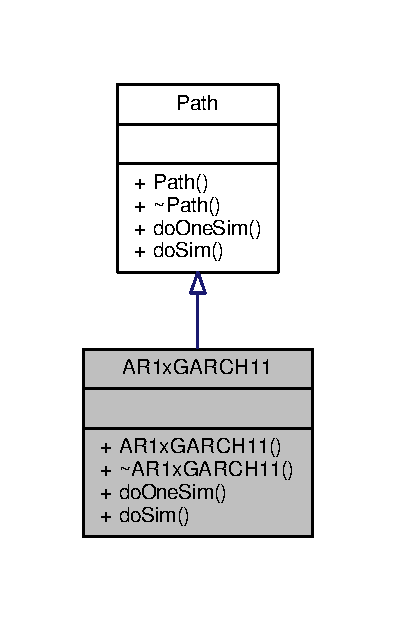
\includegraphics[width=190pt]{classAR1xGARCH11__inherit__graph}
\end{center}
\end{figure}


Collaboration diagram for A\+R1x\+G\+A\+R\+C\+H11\+:
\nopagebreak
\begin{figure}[H]
\begin{center}
\leavevmode
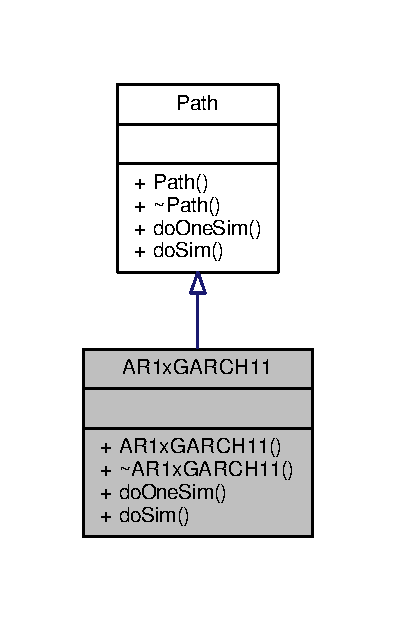
\includegraphics[width=190pt]{classAR1xGARCH11__coll__graph}
\end{center}
\end{figure}
\subsection*{Public Member Functions}
\begin{DoxyCompactItemize}
\item 
\hyperlink{classAR1xGARCH11_a898a633f6b9355bf3ccc37ba474db360}{A\+R1x\+G\+A\+R\+C\+H11} (double \+\_\+mu=0., double \+\_\+correl=0.\+5, double \+\_\+alpha=0., double \+\_\+beta=.\+24, double \+\_\+gamma=.\+76)
\item 
virtual \hyperlink{classAR1xGARCH11_acac929ce4afd12e7b0361d2e19b74fe0}{$\sim$\+A\+R1x\+G\+A\+R\+C\+H11} ()
\item 
virtual double \hyperlink{classAR1xGARCH11_ac30812d6e8339c48abcd5c0ce8ea0081}{do\+One\+Sim} (const double \&u, const double \&Sigmat, const double \&Returnt, const double \&Returntminus1) const
\item 
virtual Eigen\+::\+Vector\+Xd \hyperlink{classAR1xGARCH11_ac97f026cefd0e8bca4bbc31100f945d7}{do\+Sim} (const \hyperlink{compute__returns__eigen_8h_a1eb6a9306ef406d7975f3cbf2e247777}{Vec} \&u, const \hyperlink{compute__returns__eigen_8h_a1eb6a9306ef406d7975f3cbf2e247777}{Vec} \&Sigmat, const \hyperlink{compute__returns__eigen_8h_a1eb6a9306ef406d7975f3cbf2e247777}{Vec} \&Returnt) const
\end{DoxyCompactItemize}


\subsection{Detailed Description}
model A\+R(1) x G\+A\+R\+C\+H(1,1) -\/ Fat tails 

\subsection{Constructor \& Destructor Documentation}
\hypertarget{classAR1xGARCH11_a898a633f6b9355bf3ccc37ba474db360}{}\label{classAR1xGARCH11_a898a633f6b9355bf3ccc37ba474db360} 
\index{A\+R1x\+G\+A\+R\+C\+H11@{A\+R1x\+G\+A\+R\+C\+H11}!A\+R1x\+G\+A\+R\+C\+H11@{A\+R1x\+G\+A\+R\+C\+H11}}
\index{A\+R1x\+G\+A\+R\+C\+H11@{A\+R1x\+G\+A\+R\+C\+H11}!A\+R1x\+G\+A\+R\+C\+H11@{A\+R1x\+G\+A\+R\+C\+H11}}
\subsubsection{\texorpdfstring{A\+R1x\+G\+A\+R\+C\+H11()}{AR1xGARCH11()}}
{\footnotesize\ttfamily A\+R1x\+G\+A\+R\+C\+H11\+::\+A\+R1x\+G\+A\+R\+C\+H11 (\begin{DoxyParamCaption}\item[{double}]{\+\_\+mu = {\ttfamily 0.},  }\item[{double}]{\+\_\+correl = {\ttfamily 0.5},  }\item[{double}]{\+\_\+alpha = {\ttfamily 0.},  }\item[{double}]{\+\_\+beta = {\ttfamily .24},  }\item[{double}]{\+\_\+gamma = {\ttfamily .76} }\end{DoxyParamCaption})}


\begin{DoxyParams}{Parameters}
{\em \+\_\+mu} & average rtn \\
\hline
{\em \+\_\+correl} & $\phi$ acf previous period \\
\hline
{\em \+\_\+alpha} & $\alpha$ G\+A\+R\+CH process \\
\hline
{\em \+\_\+beta} & $\beta$ G\+A\+R\+CH process \\
\hline
{\em \+\_\+gamma} & $\gamma$ G\+A\+R\+CH process \\
\hline
\end{DoxyParams}
\hypertarget{classAR1xGARCH11_acac929ce4afd12e7b0361d2e19b74fe0}{}\label{classAR1xGARCH11_acac929ce4afd12e7b0361d2e19b74fe0} 
\index{A\+R1x\+G\+A\+R\+C\+H11@{A\+R1x\+G\+A\+R\+C\+H11}!````~A\+R1x\+G\+A\+R\+C\+H11@{$\sim$\+A\+R1x\+G\+A\+R\+C\+H11}}
\index{````~A\+R1x\+G\+A\+R\+C\+H11@{$\sim$\+A\+R1x\+G\+A\+R\+C\+H11}!A\+R1x\+G\+A\+R\+C\+H11@{A\+R1x\+G\+A\+R\+C\+H11}}
\subsubsection{\texorpdfstring{$\sim$\+A\+R1x\+G\+A\+R\+C\+H11()}{~AR1xGARCH11()}}
{\footnotesize\ttfamily virtual A\+R1x\+G\+A\+R\+C\+H11\+::$\sim$\+A\+R1x\+G\+A\+R\+C\+H11 (\begin{DoxyParamCaption}{ }\end{DoxyParamCaption})\hspace{0.3cm}{\ttfamily [inline]}, {\ttfamily [virtual]}}



\subsection{Member Function Documentation}
\hypertarget{classAR1xGARCH11_ac30812d6e8339c48abcd5c0ce8ea0081}{}\label{classAR1xGARCH11_ac30812d6e8339c48abcd5c0ce8ea0081} 
\index{A\+R1x\+G\+A\+R\+C\+H11@{A\+R1x\+G\+A\+R\+C\+H11}!do\+One\+Sim@{do\+One\+Sim}}
\index{do\+One\+Sim@{do\+One\+Sim}!A\+R1x\+G\+A\+R\+C\+H11@{A\+R1x\+G\+A\+R\+C\+H11}}
\subsubsection{\texorpdfstring{do\+One\+Sim()}{doOneSim()}}
{\footnotesize\ttfamily virtual double A\+R1x\+G\+A\+R\+C\+H11\+::do\+One\+Sim (\begin{DoxyParamCaption}\item[{const double \&}]{u,  }\item[{const double \&}]{Sigmat,  }\item[{const double \&}]{Returnt,  }\item[{const double \&}]{Returntminus1 }\end{DoxyParamCaption}) const\hspace{0.3cm}{\ttfamily [virtual]}}

Simulate return for next period under review 
\begin{DoxyParams}{Parameters}
{\em Returntminus1} & $r_{t-1}$ return previous period \\
\hline
{\em Sigmatminus1} & $\sigma_{t-1}$ vol previous period \\
\hline
{\em u} & innovation drawn sample distr. \\
\hline
{\em v} & innovation drawn sample distr. \\
\hline
\end{DoxyParams}


Implements \hyperlink{classPath_a6e75e5a329c48cafecd03a355f90b694}{Path}.

\hypertarget{classAR1xGARCH11_ac97f026cefd0e8bca4bbc31100f945d7}{}\label{classAR1xGARCH11_ac97f026cefd0e8bca4bbc31100f945d7} 
\index{A\+R1x\+G\+A\+R\+C\+H11@{A\+R1x\+G\+A\+R\+C\+H11}!do\+Sim@{do\+Sim}}
\index{do\+Sim@{do\+Sim}!A\+R1x\+G\+A\+R\+C\+H11@{A\+R1x\+G\+A\+R\+C\+H11}}
\subsubsection{\texorpdfstring{do\+Sim()}{doSim()}}
{\footnotesize\ttfamily virtual Eigen\+::\+Vector\+Xd A\+R1x\+G\+A\+R\+C\+H11\+::do\+Sim (\begin{DoxyParamCaption}\item[{const \hyperlink{compute__returns__eigen_8h_a1eb6a9306ef406d7975f3cbf2e247777}{Vec} \&}]{u,  }\item[{const \hyperlink{compute__returns__eigen_8h_a1eb6a9306ef406d7975f3cbf2e247777}{Vec} \&}]{Sigmat,  }\item[{const \hyperlink{compute__returns__eigen_8h_a1eb6a9306ef406d7975f3cbf2e247777}{Vec} \&}]{Returnt }\end{DoxyParamCaption}) const\hspace{0.3cm}{\ttfamily [virtual]}}



Implements \hyperlink{classPath_a8917612a585bce52dbd52b1b643a517a}{Path}.



The documentation for this class was generated from the following file\+:\begin{DoxyCompactItemize}
\item 
\hyperlink{path_8h}{path.\+h}\end{DoxyCompactItemize}

\hypertarget{classBootstrap}{}\section{Bootstrap$<$ T, U $>$ Class Template Reference}
\label{classBootstrap}\index{Bootstrap$<$ T, U $>$@{Bootstrap$<$ T, U $>$}}


{\ttfamily \#include $<$bootstrap.\+h$>$}



Collaboration diagram for Bootstrap$<$ T, U $>$\+:
\nopagebreak
\begin{figure}[H]
\begin{center}
\leavevmode
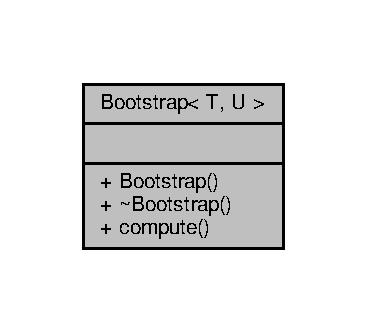
\includegraphics[width=176pt]{classBootstrap__coll__graph}
\end{center}
\end{figure}
\subsection*{Public Member Functions}
\begin{DoxyCompactItemize}
\item 
\hyperlink{classBootstrap_a35eb4a8e35d20976bd01125462192e33}{Bootstrap} ()
\item 
\hyperlink{classBootstrap_aabc424eb11af216716a5ce6169953b26}{$\sim$\+Bootstrap} ()
\item 
std\+::pair$<$ double, double $>$ \hyperlink{classBootstrap_a2b25d49ce7f6e289974a0d6b3a019581}{compute} (shared\+\_\+ptr$<$ T $>$ \&\+\_\+cr, const U \&model, size\+\_\+t p, double n\+Sim=1e+4)
\begin{DoxyCompactList}\small\item\em compute mean and standard error of \hyperlink{classVaR}{VaR} estimate through bootstrap \end{DoxyCompactList}\end{DoxyCompactItemize}


\subsection{Detailed Description}
\subsubsection*{template$<$class T, class U$>$\newline
class Bootstrap$<$ T, U $>$}

Compute historical \hyperlink{classVaR}{VaR} with bootstrap resampling


\begin{DoxyParams}{Parameters}
{\em U} & \hyperlink{classVaR}{VaR} model \\
\hline
{\em T} & compute return, portfolio \\
\hline
\end{DoxyParams}


\subsection{Constructor \& Destructor Documentation}
\hypertarget{classBootstrap_a35eb4a8e35d20976bd01125462192e33}{}\label{classBootstrap_a35eb4a8e35d20976bd01125462192e33} 
\index{Bootstrap@{Bootstrap}!Bootstrap@{Bootstrap}}
\index{Bootstrap@{Bootstrap}!Bootstrap@{Bootstrap}}
\subsubsection{\texorpdfstring{Bootstrap()}{Bootstrap()}}
{\footnotesize\ttfamily template$<$class T , class U $>$ \\
\hyperlink{classBootstrap}{Bootstrap}$<$ T, U $>$\+::\hyperlink{classBootstrap}{Bootstrap} (\begin{DoxyParamCaption}{ }\end{DoxyParamCaption})\hspace{0.3cm}{\ttfamily [inline]}}

\hypertarget{classBootstrap_aabc424eb11af216716a5ce6169953b26}{}\label{classBootstrap_aabc424eb11af216716a5ce6169953b26} 
\index{Bootstrap@{Bootstrap}!````~Bootstrap@{$\sim$\+Bootstrap}}
\index{````~Bootstrap@{$\sim$\+Bootstrap}!Bootstrap@{Bootstrap}}
\subsubsection{\texorpdfstring{$\sim$\+Bootstrap()}{~Bootstrap()}}
{\footnotesize\ttfamily template$<$class T , class U $>$ \\
\hyperlink{classBootstrap}{Bootstrap}$<$ T, U $>$\+::$\sim$\hyperlink{classBootstrap}{Bootstrap} (\begin{DoxyParamCaption}{ }\end{DoxyParamCaption})\hspace{0.3cm}{\ttfamily [inline]}}



\subsection{Member Function Documentation}
\hypertarget{classBootstrap_a2b25d49ce7f6e289974a0d6b3a019581}{}\label{classBootstrap_a2b25d49ce7f6e289974a0d6b3a019581} 
\index{Bootstrap@{Bootstrap}!compute@{compute}}
\index{compute@{compute}!Bootstrap@{Bootstrap}}
\subsubsection{\texorpdfstring{compute()}{compute()}}
{\footnotesize\ttfamily template$<$class T , class U $>$ \\
std\+::pair$<$double,double$>$ \hyperlink{classBootstrap}{Bootstrap}$<$ T, U $>$\+::compute (\begin{DoxyParamCaption}\item[{shared\+\_\+ptr$<$ T $>$ \&}]{\+\_\+cr,  }\item[{const U \&}]{model,  }\item[{size\+\_\+t}]{p,  }\item[{double}]{n\+Sim = {\ttfamily 1e+4} }\end{DoxyParamCaption})\hspace{0.3cm}{\ttfamily [inline]}}



compute mean and standard error of \hyperlink{classVaR}{VaR} estimate through bootstrap 


\begin{DoxyParams}{Parameters}
{\em \+\_\+cr} & T class (compute return, portfolio) \\
\hline
{\em model} & U class (\hyperlink{classVaR}{VaR} model) \\
\hline
{\em n\+Sim} & number of sample drawn \\
\hline
\end{DoxyParams}
\begin{DoxyReturn}{Returns}
mean and standard error of \hyperlink{classVaR}{VaR} estimate 
\end{DoxyReturn}


The documentation for this class was generated from the following file\+:\begin{DoxyCompactItemize}
\item 
\hyperlink{bootstrap_8h}{bootstrap.\+h}\end{DoxyCompactItemize}

\hypertarget{classComputeReturn}{}\section{Compute\+Return Class Reference}
\label{classComputeReturn}\index{Compute\+Return@{Compute\+Return}}


{\ttfamily \#include $<$compute\+\_\+returns\+\_\+eigen.\+h$>$}



Collaboration diagram for Compute\+Return\+:
\nopagebreak
\begin{figure}[H]
\begin{center}
\leavevmode
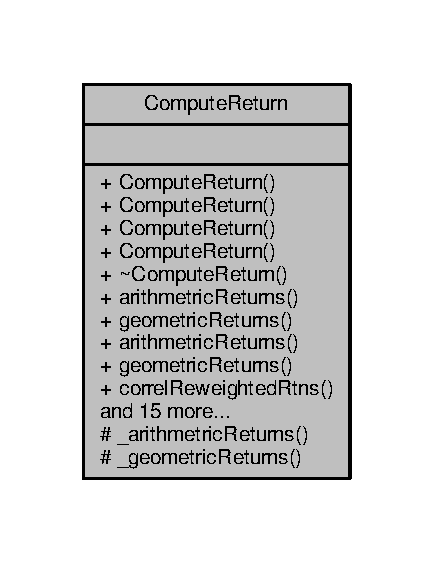
\includegraphics[width=208pt]{classComputeReturn__coll__graph}
\end{center}
\end{figure}
\subsection*{Public Member Functions}
\begin{DoxyCompactItemize}
\item 
\hyperlink{classComputeReturn_a5ddfc65ef8a500beffff33cc3f416271}{Compute\+Return} (unsigned int \+\_\+period=1, unsigned int \+\_\+k=252)
\item 
\hyperlink{classComputeReturn_a8431159bc745ac489ae4c813bd34e540}{Compute\+Return} (const \hyperlink{compute__returns__eigen_8h_a1eb6a9306ef406d7975f3cbf2e247777}{Vec} \&\+\_\+prices, unsigned int \+\_\+period=1, unsigned int \+\_\+k=252, bool \+\_\+log\+Rtns=false)
\item 
\hyperlink{classComputeReturn_a2e58c2c7e9d0f2735ceb9fdcdf0dcdde}{Compute\+Return} (const \hyperlink{compute__returns__eigen_8h_ae14dd28696f743e067dbd2594616bad6}{Mat} \&\+\_\+prices, unsigned int \+\_\+period=1, unsigned int \+\_\+k=252, bool \+\_\+log\+Rtns=false)
\item 
\hyperlink{classComputeReturn_aa737a4b9280f349201191db08e95ce9a}{Compute\+Return} (const \hyperlink{classComputeReturn}{Compute\+Return} \&other)
\begin{DoxyCompactList}\small\item\em copy constructor implementation \end{DoxyCompactList}\item 
\hyperlink{classComputeReturn_adf0a518447b70fd8990c2e06be3edb1b}{$\sim$\+Compute\+Return} ()
\item 
void \hyperlink{classComputeReturn_a3a6c9c21aa99b02dc6f2efd2b32091b8}{arithmetric\+Returns} (const \hyperlink{compute__returns__eigen_8h_a1eb6a9306ef406d7975f3cbf2e247777}{Vec} \&\+\_\+prices)
\begin{DoxyCompactList}\small\item\em compute arithmetic rtns \end{DoxyCompactList}\item 
void \hyperlink{classComputeReturn_a6c7c54511bec213c7359e041ec469e78}{geometric\+Returns} (const \hyperlink{compute__returns__eigen_8h_a1eb6a9306ef406d7975f3cbf2e247777}{Vec} \&\+\_\+prices)
\begin{DoxyCompactList}\small\item\em compute geometric rtns ie. log return \end{DoxyCompactList}\item 
void \hyperlink{classComputeReturn_a8c26c2417285e0d00204ac97b16ea05b}{arithmetric\+Returns} (const \hyperlink{compute__returns__eigen_8h_ae14dd28696f743e067dbd2594616bad6}{Mat} \&\+\_\+prices)
\item 
void \hyperlink{classComputeReturn_a2d55b2a2037f25e9a7a617af91b56272}{geometric\+Returns} (const \hyperlink{compute__returns__eigen_8h_ae14dd28696f743e067dbd2594616bad6}{Mat} \&\+\_\+prices)
\item 
void \hyperlink{classComputeReturn_a4d0b2d72a0fab11c03eb3e09f089a4b9}{correl\+Reweighted\+Rtns} (const Eigen\+::\+Matrix\+Xd \&Chat)
\begin{DoxyCompactList}\small\item\em Compute adjusted return $ \hat{R}= \hat{A} A^{-1} R$. \end{DoxyCompactList}\item 
Eigen\+::\+Matrix\+Xd \hyperlink{classComputeReturn_aef7572244a63c71bc4da1467cea38da2}{compute\+PC} ()
\begin{DoxyCompactList}\small\item\em Compute P\+CA Principal Component Analysis. \end{DoxyCompactList}\item 
\hyperlink{compute__returns__eigen_8h_a1eb6a9306ef406d7975f3cbf2e247777}{Vec} \hyperlink{classComputeReturn_a9e5d3161d117ea54508c5b4847bec4c2}{get\+Rolling\+Mean} (size\+\_\+t p) const
\begin{DoxyCompactList}\small\item\em Compute rolling mean rtn, and std dev according to period ie day, week, month and window. \end{DoxyCompactList}\item 
\hyperlink{compute__returns__eigen_8h_a1eb6a9306ef406d7975f3cbf2e247777}{Vec} \hyperlink{classComputeReturn_a3da2b36268c86dd0ea45439c7a2aa6f2}{get\+Rolling\+Std\+Dev} (size\+\_\+t p) const
\begin{DoxyCompactList}\small\item\em Compute rolling mean rtn, and std dev according to period ie day, week, month and window. \end{DoxyCompactList}\item 
unsigned int \hyperlink{classComputeReturn_a5a47d689a1f989932511663b6ec59aa6}{get\+Period} () const
\item 
unsigned int \hyperlink{classComputeReturn_a8b65977d4a7f929db92cf33c05428707}{get\+Window} () const
\item 
\hyperlink{compute__returns__eigen_8h_a1eb6a9306ef406d7975f3cbf2e247777}{Vec} \hyperlink{classComputeReturn_a9876c0984f83ab96da90e883270171bb}{get\+Returns} (size\+\_\+t p) const
\item 
\hyperlink{compute__returns__eigen_8h_ae14dd28696f743e067dbd2594616bad6}{Mat} \hyperlink{classComputeReturn_aa5389b3d2e175250e3569c996b5c7f00}{get\+Returns} () const
\item 
double \hyperlink{classComputeReturn_ab83426d16e1c870e18278db3d6b4deeb}{get\+Mean\+Return} (size\+\_\+t p=0) const
\item 
\hyperlink{compute__returns__eigen_8h_a1eb6a9306ef406d7975f3cbf2e247777}{Vec} \hyperlink{classComputeReturn_a4ea1191d38980ccebc6603e4f4fb7dce}{get\+Mean\+Returns} () const
\item 
double \hyperlink{classComputeReturn_a7aac48c9abb168e956412bf9d509cb35}{get\+Std\+Dev} (size\+\_\+t p=0) const
\item 
Eigen\+::\+Matrix\+Xd \hyperlink{classComputeReturn_a3d312fabfda99b5405e7aeab2af2fc8c}{get\+Var\+Cov} () const
\item 
Eigen\+::\+Matrix\+Xd \hyperlink{classComputeReturn_a16b185325ca2cb87991b6db59aa63de8}{get\+Correl\+Mat} ()
\item 
void \hyperlink{classComputeReturn_a6250a32e8ac308d3642bb81154ceb785}{set\+Period} (unsigned int \+\_\+period)
\item 
void \hyperlink{classComputeReturn_ae4ae713d72c4015860a8e562dfd51e75}{set\+Window} (unsigned int \+\_\+k)
\item 
void \hyperlink{classComputeReturn_ae0594e2da22ca9c96a4ce4f3eebc41eb}{set\+Returns} (const \hyperlink{compute__returns__eigen_8h_ae14dd28696f743e067dbd2594616bad6}{Mat} \&\+\_\+m\+Asset\+Returns)
\end{DoxyCompactItemize}
\subsection*{Protected Member Functions}
\begin{DoxyCompactItemize}
\item 
void \hyperlink{classComputeReturn_a80678bbba59305a392d001260fb2d32b}{\+\_\+arithmetric\+Returns} (size\+\_\+t j=0)
\begin{DoxyCompactList}\small\item\em compute arithmetic rtns \end{DoxyCompactList}\item 
void \hyperlink{classComputeReturn_a9738eae9cbcbe4d75a86335d95adc758}{\+\_\+geometric\+Returns} (size\+\_\+t j=0)
\begin{DoxyCompactList}\small\item\em compute geometric rtns ie. log return \end{DoxyCompactList}\end{DoxyCompactItemize}


\subsection{Detailed Description}
Compute returns, mean, std dev

Assume daily return 

\subsection{Constructor \& Destructor Documentation}
\hypertarget{classComputeReturn_a5ddfc65ef8a500beffff33cc3f416271}{}\label{classComputeReturn_a5ddfc65ef8a500beffff33cc3f416271} 
\index{Compute\+Return@{Compute\+Return}!Compute\+Return@{Compute\+Return}}
\index{Compute\+Return@{Compute\+Return}!Compute\+Return@{Compute\+Return}}
\subsubsection{\texorpdfstring{Compute\+Return()}{ComputeReturn()}\hspace{0.1cm}{\footnotesize\ttfamily [1/4]}}
{\footnotesize\ttfamily Compute\+Return\+::\+Compute\+Return (\begin{DoxyParamCaption}\item[{unsigned int}]{\+\_\+period = {\ttfamily 1},  }\item[{unsigned int}]{\+\_\+k = {\ttfamily 252} }\end{DoxyParamCaption})}

constructor 2X overloads 
\begin{DoxyParams}{Parameters}
{\em period} & one day. 252 trading days (US trading calendar) \\
\hline
{\em k} & rolling period. 1 year \\
\hline
\end{DoxyParams}
\hypertarget{classComputeReturn_a8431159bc745ac489ae4c813bd34e540}{}\label{classComputeReturn_a8431159bc745ac489ae4c813bd34e540} 
\index{Compute\+Return@{Compute\+Return}!Compute\+Return@{Compute\+Return}}
\index{Compute\+Return@{Compute\+Return}!Compute\+Return@{Compute\+Return}}
\subsubsection{\texorpdfstring{Compute\+Return()}{ComputeReturn()}\hspace{0.1cm}{\footnotesize\ttfamily [2/4]}}
{\footnotesize\ttfamily Compute\+Return\+::\+Compute\+Return (\begin{DoxyParamCaption}\item[{const \hyperlink{compute__returns__eigen_8h_a1eb6a9306ef406d7975f3cbf2e247777}{Vec} \&}]{\+\_\+prices,  }\item[{unsigned int}]{\+\_\+period = {\ttfamily 1},  }\item[{unsigned int}]{\+\_\+k = {\ttfamily 252},  }\item[{bool}]{\+\_\+log\+Rtns = {\ttfamily false} }\end{DoxyParamCaption})}

\hypertarget{classComputeReturn_a2e58c2c7e9d0f2735ceb9fdcdf0dcdde}{}\label{classComputeReturn_a2e58c2c7e9d0f2735ceb9fdcdf0dcdde} 
\index{Compute\+Return@{Compute\+Return}!Compute\+Return@{Compute\+Return}}
\index{Compute\+Return@{Compute\+Return}!Compute\+Return@{Compute\+Return}}
\subsubsection{\texorpdfstring{Compute\+Return()}{ComputeReturn()}\hspace{0.1cm}{\footnotesize\ttfamily [3/4]}}
{\footnotesize\ttfamily Compute\+Return\+::\+Compute\+Return (\begin{DoxyParamCaption}\item[{const \hyperlink{compute__returns__eigen_8h_ae14dd28696f743e067dbd2594616bad6}{Mat} \&}]{\+\_\+prices,  }\item[{unsigned int}]{\+\_\+period = {\ttfamily 1},  }\item[{unsigned int}]{\+\_\+k = {\ttfamily 252},  }\item[{bool}]{\+\_\+log\+Rtns = {\ttfamily false} }\end{DoxyParamCaption})}

\hypertarget{classComputeReturn_aa737a4b9280f349201191db08e95ce9a}{}\label{classComputeReturn_aa737a4b9280f349201191db08e95ce9a} 
\index{Compute\+Return@{Compute\+Return}!Compute\+Return@{Compute\+Return}}
\index{Compute\+Return@{Compute\+Return}!Compute\+Return@{Compute\+Return}}
\subsubsection{\texorpdfstring{Compute\+Return()}{ComputeReturn()}\hspace{0.1cm}{\footnotesize\ttfamily [4/4]}}
{\footnotesize\ttfamily Compute\+Return\+::\+Compute\+Return (\begin{DoxyParamCaption}\item[{const \hyperlink{classComputeReturn}{Compute\+Return} \&}]{other }\end{DoxyParamCaption})}



copy constructor implementation 

\hypertarget{classComputeReturn_adf0a518447b70fd8990c2e06be3edb1b}{}\label{classComputeReturn_adf0a518447b70fd8990c2e06be3edb1b} 
\index{Compute\+Return@{Compute\+Return}!````~Compute\+Return@{$\sim$\+Compute\+Return}}
\index{````~Compute\+Return@{$\sim$\+Compute\+Return}!Compute\+Return@{Compute\+Return}}
\subsubsection{\texorpdfstring{$\sim$\+Compute\+Return()}{~ComputeReturn()}}
{\footnotesize\ttfamily Compute\+Return\+::$\sim$\+Compute\+Return (\begin{DoxyParamCaption}{ }\end{DoxyParamCaption})\hspace{0.3cm}{\ttfamily [inline]}}



\subsection{Member Function Documentation}
\hypertarget{classComputeReturn_a80678bbba59305a392d001260fb2d32b}{}\label{classComputeReturn_a80678bbba59305a392d001260fb2d32b} 
\index{Compute\+Return@{Compute\+Return}!\+\_\+arithmetric\+Returns@{\+\_\+arithmetric\+Returns}}
\index{\+\_\+arithmetric\+Returns@{\+\_\+arithmetric\+Returns}!Compute\+Return@{Compute\+Return}}
\subsubsection{\texorpdfstring{\+\_\+arithmetric\+Returns()}{\_arithmetricReturns()}}
{\footnotesize\ttfamily void Compute\+Return\+::\+\_\+arithmetric\+Returns (\begin{DoxyParamCaption}\item[{size\+\_\+t}]{j = {\ttfamily 0} }\end{DoxyParamCaption})\hspace{0.3cm}{\ttfamily [inline]}, {\ttfamily [protected]}}



compute arithmetic rtns 

\hypertarget{classComputeReturn_a9738eae9cbcbe4d75a86335d95adc758}{}\label{classComputeReturn_a9738eae9cbcbe4d75a86335d95adc758} 
\index{Compute\+Return@{Compute\+Return}!\+\_\+geometric\+Returns@{\+\_\+geometric\+Returns}}
\index{\+\_\+geometric\+Returns@{\+\_\+geometric\+Returns}!Compute\+Return@{Compute\+Return}}
\subsubsection{\texorpdfstring{\+\_\+geometric\+Returns()}{\_geometricReturns()}}
{\footnotesize\ttfamily void Compute\+Return\+::\+\_\+geometric\+Returns (\begin{DoxyParamCaption}\item[{size\+\_\+t}]{j = {\ttfamily 0} }\end{DoxyParamCaption})\hspace{0.3cm}{\ttfamily [inline]}, {\ttfamily [protected]}}



compute geometric rtns ie. log return 

\hypertarget{classComputeReturn_a3a6c9c21aa99b02dc6f2efd2b32091b8}{}\label{classComputeReturn_a3a6c9c21aa99b02dc6f2efd2b32091b8} 
\index{Compute\+Return@{Compute\+Return}!arithmetric\+Returns@{arithmetric\+Returns}}
\index{arithmetric\+Returns@{arithmetric\+Returns}!Compute\+Return@{Compute\+Return}}
\subsubsection{\texorpdfstring{arithmetric\+Returns()}{arithmetricReturns()}\hspace{0.1cm}{\footnotesize\ttfamily [1/2]}}
{\footnotesize\ttfamily void Compute\+Return\+::arithmetric\+Returns (\begin{DoxyParamCaption}\item[{const \hyperlink{compute__returns__eigen_8h_a1eb6a9306ef406d7975f3cbf2e247777}{Vec} \&}]{\+\_\+prices }\end{DoxyParamCaption})}



compute arithmetic rtns 

\hypertarget{classComputeReturn_a8c26c2417285e0d00204ac97b16ea05b}{}\label{classComputeReturn_a8c26c2417285e0d00204ac97b16ea05b} 
\index{Compute\+Return@{Compute\+Return}!arithmetric\+Returns@{arithmetric\+Returns}}
\index{arithmetric\+Returns@{arithmetric\+Returns}!Compute\+Return@{Compute\+Return}}
\subsubsection{\texorpdfstring{arithmetric\+Returns()}{arithmetricReturns()}\hspace{0.1cm}{\footnotesize\ttfamily [2/2]}}
{\footnotesize\ttfamily void Compute\+Return\+::arithmetric\+Returns (\begin{DoxyParamCaption}\item[{const \hyperlink{compute__returns__eigen_8h_ae14dd28696f743e067dbd2594616bad6}{Mat} \&}]{\+\_\+prices }\end{DoxyParamCaption})}

\hypertarget{classComputeReturn_aef7572244a63c71bc4da1467cea38da2}{}\label{classComputeReturn_aef7572244a63c71bc4da1467cea38da2} 
\index{Compute\+Return@{Compute\+Return}!compute\+PC@{compute\+PC}}
\index{compute\+PC@{compute\+PC}!Compute\+Return@{Compute\+Return}}
\subsubsection{\texorpdfstring{compute\+P\+C()}{computePC()}}
{\footnotesize\ttfamily Eigen\+::\+Matrix\+Xd Compute\+Return\+::compute\+PC (\begin{DoxyParamCaption}{ }\end{DoxyParamCaption})}



Compute P\+CA Principal Component Analysis. 

Principal Component up to 99\% \hypertarget{classComputeReturn_a4d0b2d72a0fab11c03eb3e09f089a4b9}{}\label{classComputeReturn_a4d0b2d72a0fab11c03eb3e09f089a4b9} 
\index{Compute\+Return@{Compute\+Return}!correl\+Reweighted\+Rtns@{correl\+Reweighted\+Rtns}}
\index{correl\+Reweighted\+Rtns@{correl\+Reweighted\+Rtns}!Compute\+Return@{Compute\+Return}}
\subsubsection{\texorpdfstring{correl\+Reweighted\+Rtns()}{correlReweightedRtns()}}
{\footnotesize\ttfamily void Compute\+Return\+::correl\+Reweighted\+Rtns (\begin{DoxyParamCaption}\item[{const Eigen\+::\+Matrix\+Xd \&}]{Chat }\end{DoxyParamCaption})}



Compute adjusted return $ \hat{R}= \hat{A} A^{-1} R$. 


\begin{DoxyParams}{Parameters}
{\em Chat} & = Bumped original correl matrix for several asset pairs\\
\hline
\end{DoxyParams}
C, Chat correlation matrices

Use Cholesky decomposition $X = LL^T$

ie.

$C = AA^T$

$ \hat{C} = \hat{A} \hat{A} ^{T}$ \hypertarget{classComputeReturn_a6c7c54511bec213c7359e041ec469e78}{}\label{classComputeReturn_a6c7c54511bec213c7359e041ec469e78} 
\index{Compute\+Return@{Compute\+Return}!geometric\+Returns@{geometric\+Returns}}
\index{geometric\+Returns@{geometric\+Returns}!Compute\+Return@{Compute\+Return}}
\subsubsection{\texorpdfstring{geometric\+Returns()}{geometricReturns()}\hspace{0.1cm}{\footnotesize\ttfamily [1/2]}}
{\footnotesize\ttfamily void Compute\+Return\+::geometric\+Returns (\begin{DoxyParamCaption}\item[{const \hyperlink{compute__returns__eigen_8h_a1eb6a9306ef406d7975f3cbf2e247777}{Vec} \&}]{\+\_\+prices }\end{DoxyParamCaption})}



compute geometric rtns ie. log return 

\hypertarget{classComputeReturn_a2d55b2a2037f25e9a7a617af91b56272}{}\label{classComputeReturn_a2d55b2a2037f25e9a7a617af91b56272} 
\index{Compute\+Return@{Compute\+Return}!geometric\+Returns@{geometric\+Returns}}
\index{geometric\+Returns@{geometric\+Returns}!Compute\+Return@{Compute\+Return}}
\subsubsection{\texorpdfstring{geometric\+Returns()}{geometricReturns()}\hspace{0.1cm}{\footnotesize\ttfamily [2/2]}}
{\footnotesize\ttfamily void Compute\+Return\+::geometric\+Returns (\begin{DoxyParamCaption}\item[{const \hyperlink{compute__returns__eigen_8h_ae14dd28696f743e067dbd2594616bad6}{Mat} \&}]{\+\_\+prices }\end{DoxyParamCaption})}

\hypertarget{classComputeReturn_a16b185325ca2cb87991b6db59aa63de8}{}\label{classComputeReturn_a16b185325ca2cb87991b6db59aa63de8} 
\index{Compute\+Return@{Compute\+Return}!get\+Correl\+Mat@{get\+Correl\+Mat}}
\index{get\+Correl\+Mat@{get\+Correl\+Mat}!Compute\+Return@{Compute\+Return}}
\subsubsection{\texorpdfstring{get\+Correl\+Mat()}{getCorrelMat()}}
{\footnotesize\ttfamily Eigen\+::\+Matrix\+Xd Compute\+Return\+::get\+Correl\+Mat (\begin{DoxyParamCaption}{ }\end{DoxyParamCaption})}

\hypertarget{classComputeReturn_ab83426d16e1c870e18278db3d6b4deeb}{}\label{classComputeReturn_ab83426d16e1c870e18278db3d6b4deeb} 
\index{Compute\+Return@{Compute\+Return}!get\+Mean\+Return@{get\+Mean\+Return}}
\index{get\+Mean\+Return@{get\+Mean\+Return}!Compute\+Return@{Compute\+Return}}
\subsubsection{\texorpdfstring{get\+Mean\+Return()}{getMeanReturn()}}
{\footnotesize\ttfamily double Compute\+Return\+::get\+Mean\+Return (\begin{DoxyParamCaption}\item[{size\+\_\+t}]{p = {\ttfamily 0} }\end{DoxyParamCaption}) const}

\hypertarget{classComputeReturn_a4ea1191d38980ccebc6603e4f4fb7dce}{}\label{classComputeReturn_a4ea1191d38980ccebc6603e4f4fb7dce} 
\index{Compute\+Return@{Compute\+Return}!get\+Mean\+Returns@{get\+Mean\+Returns}}
\index{get\+Mean\+Returns@{get\+Mean\+Returns}!Compute\+Return@{Compute\+Return}}
\subsubsection{\texorpdfstring{get\+Mean\+Returns()}{getMeanReturns()}}
{\footnotesize\ttfamily \hyperlink{compute__returns__eigen_8h_a1eb6a9306ef406d7975f3cbf2e247777}{Vec} Compute\+Return\+::get\+Mean\+Returns (\begin{DoxyParamCaption}{ }\end{DoxyParamCaption}) const\hspace{0.3cm}{\ttfamily [inline]}}

\hypertarget{classComputeReturn_a5a47d689a1f989932511663b6ec59aa6}{}\label{classComputeReturn_a5a47d689a1f989932511663b6ec59aa6} 
\index{Compute\+Return@{Compute\+Return}!get\+Period@{get\+Period}}
\index{get\+Period@{get\+Period}!Compute\+Return@{Compute\+Return}}
\subsubsection{\texorpdfstring{get\+Period()}{getPeriod()}}
{\footnotesize\ttfamily unsigned int Compute\+Return\+::get\+Period (\begin{DoxyParamCaption}{ }\end{DoxyParamCaption}) const\hspace{0.3cm}{\ttfamily [inline]}}

\hypertarget{classComputeReturn_a9876c0984f83ab96da90e883270171bb}{}\label{classComputeReturn_a9876c0984f83ab96da90e883270171bb} 
\index{Compute\+Return@{Compute\+Return}!get\+Returns@{get\+Returns}}
\index{get\+Returns@{get\+Returns}!Compute\+Return@{Compute\+Return}}
\subsubsection{\texorpdfstring{get\+Returns()}{getReturns()}\hspace{0.1cm}{\footnotesize\ttfamily [1/2]}}
{\footnotesize\ttfamily \hyperlink{compute__returns__eigen_8h_a1eb6a9306ef406d7975f3cbf2e247777}{Vec} Compute\+Return\+::get\+Returns (\begin{DoxyParamCaption}\item[{size\+\_\+t}]{p }\end{DoxyParamCaption}) const}

\hypertarget{classComputeReturn_aa5389b3d2e175250e3569c996b5c7f00}{}\label{classComputeReturn_aa5389b3d2e175250e3569c996b5c7f00} 
\index{Compute\+Return@{Compute\+Return}!get\+Returns@{get\+Returns}}
\index{get\+Returns@{get\+Returns}!Compute\+Return@{Compute\+Return}}
\subsubsection{\texorpdfstring{get\+Returns()}{getReturns()}\hspace{0.1cm}{\footnotesize\ttfamily [2/2]}}
{\footnotesize\ttfamily \hyperlink{compute__returns__eigen_8h_ae14dd28696f743e067dbd2594616bad6}{Mat} Compute\+Return\+::get\+Returns (\begin{DoxyParamCaption}{ }\end{DoxyParamCaption}) const\hspace{0.3cm}{\ttfamily [inline]}}

\hypertarget{classComputeReturn_a9e5d3161d117ea54508c5b4847bec4c2}{}\label{classComputeReturn_a9e5d3161d117ea54508c5b4847bec4c2} 
\index{Compute\+Return@{Compute\+Return}!get\+Rolling\+Mean@{get\+Rolling\+Mean}}
\index{get\+Rolling\+Mean@{get\+Rolling\+Mean}!Compute\+Return@{Compute\+Return}}
\subsubsection{\texorpdfstring{get\+Rolling\+Mean()}{getRollingMean()}}
{\footnotesize\ttfamily \hyperlink{compute__returns__eigen_8h_a1eb6a9306ef406d7975f3cbf2e247777}{Vec} Compute\+Return\+::get\+Rolling\+Mean (\begin{DoxyParamCaption}\item[{size\+\_\+t}]{p }\end{DoxyParamCaption}) const}



Compute rolling mean rtn, and std dev according to period ie day, week, month and window. 

\hypertarget{classComputeReturn_a3da2b36268c86dd0ea45439c7a2aa6f2}{}\label{classComputeReturn_a3da2b36268c86dd0ea45439c7a2aa6f2} 
\index{Compute\+Return@{Compute\+Return}!get\+Rolling\+Std\+Dev@{get\+Rolling\+Std\+Dev}}
\index{get\+Rolling\+Std\+Dev@{get\+Rolling\+Std\+Dev}!Compute\+Return@{Compute\+Return}}
\subsubsection{\texorpdfstring{get\+Rolling\+Std\+Dev()}{getRollingStdDev()}}
{\footnotesize\ttfamily \hyperlink{compute__returns__eigen_8h_a1eb6a9306ef406d7975f3cbf2e247777}{Vec} Compute\+Return\+::get\+Rolling\+Std\+Dev (\begin{DoxyParamCaption}\item[{size\+\_\+t}]{p }\end{DoxyParamCaption}) const}



Compute rolling mean rtn, and std dev according to period ie day, week, month and window. 

\hypertarget{classComputeReturn_a7aac48c9abb168e956412bf9d509cb35}{}\label{classComputeReturn_a7aac48c9abb168e956412bf9d509cb35} 
\index{Compute\+Return@{Compute\+Return}!get\+Std\+Dev@{get\+Std\+Dev}}
\index{get\+Std\+Dev@{get\+Std\+Dev}!Compute\+Return@{Compute\+Return}}
\subsubsection{\texorpdfstring{get\+Std\+Dev()}{getStdDev()}}
{\footnotesize\ttfamily double Compute\+Return\+::get\+Std\+Dev (\begin{DoxyParamCaption}\item[{size\+\_\+t}]{p = {\ttfamily 0} }\end{DoxyParamCaption}) const}

\hypertarget{classComputeReturn_a3d312fabfda99b5405e7aeab2af2fc8c}{}\label{classComputeReturn_a3d312fabfda99b5405e7aeab2af2fc8c} 
\index{Compute\+Return@{Compute\+Return}!get\+Var\+Cov@{get\+Var\+Cov}}
\index{get\+Var\+Cov@{get\+Var\+Cov}!Compute\+Return@{Compute\+Return}}
\subsubsection{\texorpdfstring{get\+Var\+Cov()}{getVarCov()}}
{\footnotesize\ttfamily Eigen\+::\+Matrix\+Xd Compute\+Return\+::get\+Var\+Cov (\begin{DoxyParamCaption}{ }\end{DoxyParamCaption}) const\hspace{0.3cm}{\ttfamily [inline]}}

\hypertarget{classComputeReturn_a8b65977d4a7f929db92cf33c05428707}{}\label{classComputeReturn_a8b65977d4a7f929db92cf33c05428707} 
\index{Compute\+Return@{Compute\+Return}!get\+Window@{get\+Window}}
\index{get\+Window@{get\+Window}!Compute\+Return@{Compute\+Return}}
\subsubsection{\texorpdfstring{get\+Window()}{getWindow()}}
{\footnotesize\ttfamily unsigned int Compute\+Return\+::get\+Window (\begin{DoxyParamCaption}{ }\end{DoxyParamCaption}) const\hspace{0.3cm}{\ttfamily [inline]}}

\hypertarget{classComputeReturn_a6250a32e8ac308d3642bb81154ceb785}{}\label{classComputeReturn_a6250a32e8ac308d3642bb81154ceb785} 
\index{Compute\+Return@{Compute\+Return}!set\+Period@{set\+Period}}
\index{set\+Period@{set\+Period}!Compute\+Return@{Compute\+Return}}
\subsubsection{\texorpdfstring{set\+Period()}{setPeriod()}}
{\footnotesize\ttfamily void Compute\+Return\+::set\+Period (\begin{DoxyParamCaption}\item[{unsigned int}]{\+\_\+period }\end{DoxyParamCaption})}

\hypertarget{classComputeReturn_ae0594e2da22ca9c96a4ce4f3eebc41eb}{}\label{classComputeReturn_ae0594e2da22ca9c96a4ce4f3eebc41eb} 
\index{Compute\+Return@{Compute\+Return}!set\+Returns@{set\+Returns}}
\index{set\+Returns@{set\+Returns}!Compute\+Return@{Compute\+Return}}
\subsubsection{\texorpdfstring{set\+Returns()}{setReturns()}}
{\footnotesize\ttfamily void Compute\+Return\+::set\+Returns (\begin{DoxyParamCaption}\item[{const \hyperlink{compute__returns__eigen_8h_ae14dd28696f743e067dbd2594616bad6}{Mat} \&}]{\+\_\+m\+Asset\+Returns }\end{DoxyParamCaption})}

\hypertarget{classComputeReturn_ae4ae713d72c4015860a8e562dfd51e75}{}\label{classComputeReturn_ae4ae713d72c4015860a8e562dfd51e75} 
\index{Compute\+Return@{Compute\+Return}!set\+Window@{set\+Window}}
\index{set\+Window@{set\+Window}!Compute\+Return@{Compute\+Return}}
\subsubsection{\texorpdfstring{set\+Window()}{setWindow()}}
{\footnotesize\ttfamily void Compute\+Return\+::set\+Window (\begin{DoxyParamCaption}\item[{unsigned int}]{\+\_\+k }\end{DoxyParamCaption})}



The documentation for this class was generated from the following file\+:\begin{DoxyCompactItemize}
\item 
\hyperlink{compute__returns__eigen_8h}{compute\+\_\+returns\+\_\+eigen.\+h}\end{DoxyCompactItemize}

\hypertarget{classCopulaEngine}{}\section{Copula\+Engine$<$ T, U $>$ Class Template Reference}
\label{classCopulaEngine}\index{Copula\+Engine$<$ T, U $>$@{Copula\+Engine$<$ T, U $>$}}


T rng, U path.  




{\ttfamily \#include $<$mc\+\_\+engine.\+h$>$}



Inheritance diagram for Copula\+Engine$<$ T, U $>$\+:
\nopagebreak
\begin{figure}[H]
\begin{center}
\leavevmode
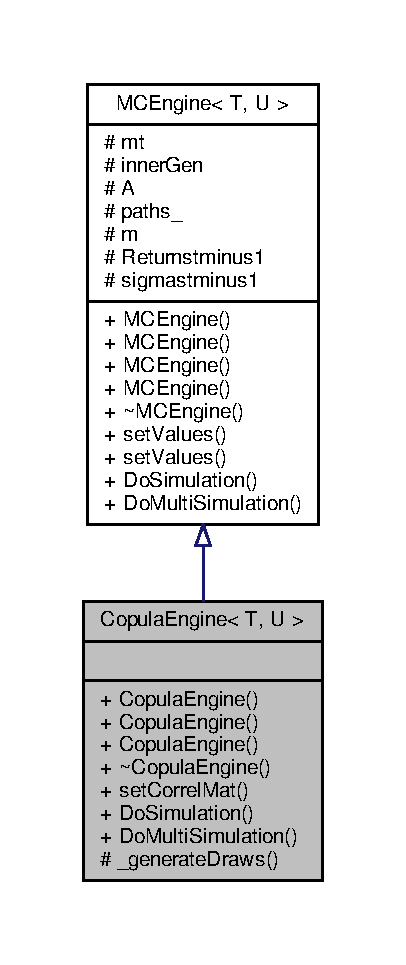
\includegraphics[width=195pt]{classCopulaEngine__inherit__graph}
\end{center}
\end{figure}


Collaboration diagram for Copula\+Engine$<$ T, U $>$\+:
\nopagebreak
\begin{figure}[H]
\begin{center}
\leavevmode
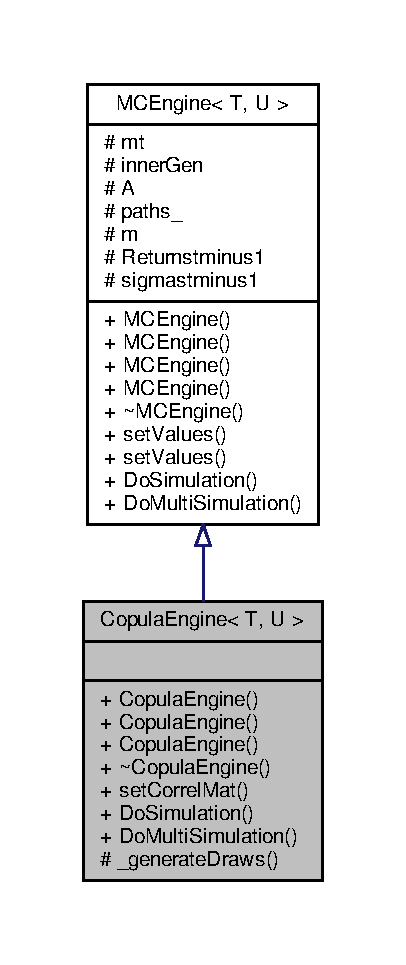
\includegraphics[width=195pt]{classCopulaEngine__coll__graph}
\end{center}
\end{figure}
\subsection*{Public Types}
\begin{DoxyCompactItemize}
\item 
typedef std\+::vector$<$ U $>$ \hyperlink{classCopulaEngine_a75e30032c9b2290243a83ea7d343a62c}{paths}
\end{DoxyCompactItemize}
\subsection*{Public Member Functions}
\begin{DoxyCompactItemize}
\item 
\hyperlink{classCopulaEngine_af3eb5649a8e86dd99de690cac3e843f1}{Copula\+Engine} (T \&\+\_\+rng\+\_\+, const \hyperlink{classMCEngine_a977f1048508a1467c496c2c47231d1d3}{paths} \&\+\_\+paths, const Eigen\+::\+Matrix\+Xd \+\_\+C)
\item 
\hyperlink{classCopulaEngine_a26fa5d1a9a5cb3fe2f406a63049fe4e9}{Copula\+Engine} (T \&\+\_\+rng\+\_\+, const \hyperlink{classMCEngine_a977f1048508a1467c496c2c47231d1d3}{paths} \&\+\_\+paths)
\item 
\hyperlink{classCopulaEngine_a2f0ff634cdaaa44f21f2ccd3c583d918}{Copula\+Engine} (const \hyperlink{classCopulaEngine}{Copula\+Engine} \&other)
\item 
virtual \hyperlink{classCopulaEngine_aadcd0c2890899853db28a2269be09745}{$\sim$\+Copula\+Engine} ()
\item 
void \hyperlink{classCopulaEngine_a0a330b7405b9cfcb205aaf6db1d954c3}{set\+Correl\+Mat} (const Eigen\+::\+Matrix\+Xd \&\+\_\+C)
\item 
\hyperlink{compute__returns__eigen_8h_a1eb6a9306ef406d7975f3cbf2e247777}{Vec} \hyperlink{classCopulaEngine_ac14e86c4f0025bcc82e680896e1c7e3a}{Do\+Simulation} (size\+\_\+t p=0, double n=1.e+05, double dof=3., double gamma=1., \hyperlink{rng_8h_aff2c6be1fded3d6d996b850e2eb87c25}{copula\+Type} ct=\hyperlink{rng_8h_aff2c6be1fded3d6d996b850e2eb87c25ab15a7891aa5223439e4692a1048cb220}{Gauss}, \hyperlink{mc__engine_8h_aeb3b337d49b67199ac031f705d206198}{underlying\+Process} ud=\hyperlink{mc__engine_8h_aeb3b337d49b67199ac031f705d206198aa11844f44df96808eb4e519ba04f088c}{Gaussian})
\item 
\hyperlink{compute__returns__eigen_8h_ae14dd28696f743e067dbd2594616bad6}{Mat} \hyperlink{classCopulaEngine_a7074287ea29264912673d2d12d38bcdc}{Do\+Multi\+Simulation} (double n=1.e+05, double dof=3., double gamma=1., \hyperlink{rng_8h_aff2c6be1fded3d6d996b850e2eb87c25}{copula\+Type} ct=\hyperlink{rng_8h_aff2c6be1fded3d6d996b850e2eb87c25ab15a7891aa5223439e4692a1048cb220}{Gauss}, \hyperlink{mc__engine_8h_aeb3b337d49b67199ac031f705d206198}{underlying\+Process} ud=\hyperlink{mc__engine_8h_aeb3b337d49b67199ac031f705d206198aa11844f44df96808eb4e519ba04f088c}{Gaussian})
\end{DoxyCompactItemize}
\subsection*{Protected Member Functions}
\begin{DoxyCompactItemize}
\item 
\hyperlink{compute__returns__eigen_8h_a1eb6a9306ef406d7975f3cbf2e247777}{Vec} \hyperlink{classCopulaEngine_a9e74792c12cbe443f77221466b851aec}{\+\_\+generate\+Draws} (\hyperlink{rng_8h_aff2c6be1fded3d6d996b850e2eb87c25}{copula\+Type} ct=\hyperlink{rng_8h_aff2c6be1fded3d6d996b850e2eb87c25ab15a7891aa5223439e4692a1048cb220}{Gauss}, double dof=3., double gamma=1.)
\end{DoxyCompactItemize}
\subsection*{Additional Inherited Members}


\subsection{Detailed Description}
\subsubsection*{template$<$class T, class U$>$\newline
class Copula\+Engine$<$ T, U $>$}

T rng, U path. 

\subsection{Member Typedef Documentation}
\hypertarget{classCopulaEngine_a75e30032c9b2290243a83ea7d343a62c}{}\label{classCopulaEngine_a75e30032c9b2290243a83ea7d343a62c} 
\index{Copula\+Engine@{Copula\+Engine}!paths@{paths}}
\index{paths@{paths}!Copula\+Engine@{Copula\+Engine}}
\subsubsection{\texorpdfstring{paths}{paths}}
{\footnotesize\ttfamily template$<$class T , class U $>$ \\
typedef std\+::vector$<$U$>$ \hyperlink{classCopulaEngine}{Copula\+Engine}$<$ T, U $>$\+::\hyperlink{classMCEngine_a977f1048508a1467c496c2c47231d1d3}{paths}}



\subsection{Constructor \& Destructor Documentation}
\hypertarget{classCopulaEngine_af3eb5649a8e86dd99de690cac3e843f1}{}\label{classCopulaEngine_af3eb5649a8e86dd99de690cac3e843f1} 
\index{Copula\+Engine@{Copula\+Engine}!Copula\+Engine@{Copula\+Engine}}
\index{Copula\+Engine@{Copula\+Engine}!Copula\+Engine@{Copula\+Engine}}
\subsubsection{\texorpdfstring{Copula\+Engine()}{CopulaEngine()}\hspace{0.1cm}{\footnotesize\ttfamily [1/3]}}
{\footnotesize\ttfamily template$<$class T , class U $>$ \\
\hyperlink{classCopulaEngine}{Copula\+Engine}$<$ T, U $>$\+::\hyperlink{classCopulaEngine}{Copula\+Engine} (\begin{DoxyParamCaption}\item[{T \&}]{\+\_\+rng\+\_\+,  }\item[{const \hyperlink{classMCEngine_a977f1048508a1467c496c2c47231d1d3}{paths} \&}]{\+\_\+paths,  }\item[{const Eigen\+::\+Matrix\+Xd}]{\+\_\+C }\end{DoxyParamCaption})\hspace{0.3cm}{\ttfamily [inline]}}

Constructor 1x overload

multiple assets


\begin{DoxyParams}{Parameters}
{\em \+\_\+rng} & pseudo random number generator \\
\hline
{\em \+\_\+paths} & paths vector \\
\hline
{\em \+\_\+C} & correlation matrix \\
\hline
\end{DoxyParams}
\hypertarget{classCopulaEngine_a26fa5d1a9a5cb3fe2f406a63049fe4e9}{}\label{classCopulaEngine_a26fa5d1a9a5cb3fe2f406a63049fe4e9} 
\index{Copula\+Engine@{Copula\+Engine}!Copula\+Engine@{Copula\+Engine}}
\index{Copula\+Engine@{Copula\+Engine}!Copula\+Engine@{Copula\+Engine}}
\subsubsection{\texorpdfstring{Copula\+Engine()}{CopulaEngine()}\hspace{0.1cm}{\footnotesize\ttfamily [2/3]}}
{\footnotesize\ttfamily template$<$class T , class U $>$ \\
\hyperlink{classCopulaEngine}{Copula\+Engine}$<$ T, U $>$\+::\hyperlink{classCopulaEngine}{Copula\+Engine} (\begin{DoxyParamCaption}\item[{T \&}]{\+\_\+rng\+\_\+,  }\item[{const \hyperlink{classMCEngine_a977f1048508a1467c496c2c47231d1d3}{paths} \&}]{\+\_\+paths }\end{DoxyParamCaption})\hspace{0.3cm}{\ttfamily [inline]}}

\hypertarget{classCopulaEngine_a2f0ff634cdaaa44f21f2ccd3c583d918}{}\label{classCopulaEngine_a2f0ff634cdaaa44f21f2ccd3c583d918} 
\index{Copula\+Engine@{Copula\+Engine}!Copula\+Engine@{Copula\+Engine}}
\index{Copula\+Engine@{Copula\+Engine}!Copula\+Engine@{Copula\+Engine}}
\subsubsection{\texorpdfstring{Copula\+Engine()}{CopulaEngine()}\hspace{0.1cm}{\footnotesize\ttfamily [3/3]}}
{\footnotesize\ttfamily template$<$class T , class U $>$ \\
\hyperlink{classCopulaEngine}{Copula\+Engine}$<$ T, U $>$\+::\hyperlink{classCopulaEngine}{Copula\+Engine} (\begin{DoxyParamCaption}\item[{const \hyperlink{classCopulaEngine}{Copula\+Engine}$<$ T, U $>$ \&}]{other }\end{DoxyParamCaption})}

\hypertarget{classCopulaEngine_aadcd0c2890899853db28a2269be09745}{}\label{classCopulaEngine_aadcd0c2890899853db28a2269be09745} 
\index{Copula\+Engine@{Copula\+Engine}!````~Copula\+Engine@{$\sim$\+Copula\+Engine}}
\index{````~Copula\+Engine@{$\sim$\+Copula\+Engine}!Copula\+Engine@{Copula\+Engine}}
\subsubsection{\texorpdfstring{$\sim$\+Copula\+Engine()}{~CopulaEngine()}}
{\footnotesize\ttfamily template$<$class T , class U $>$ \\
virtual \hyperlink{classCopulaEngine}{Copula\+Engine}$<$ T, U $>$\+::$\sim$\hyperlink{classCopulaEngine}{Copula\+Engine} (\begin{DoxyParamCaption}{ }\end{DoxyParamCaption})\hspace{0.3cm}{\ttfamily [inline]}, {\ttfamily [virtual]}}



\subsection{Member Function Documentation}
\hypertarget{classCopulaEngine_a9e74792c12cbe443f77221466b851aec}{}\label{classCopulaEngine_a9e74792c12cbe443f77221466b851aec} 
\index{Copula\+Engine@{Copula\+Engine}!\+\_\+generate\+Draws@{\+\_\+generate\+Draws}}
\index{\+\_\+generate\+Draws@{\+\_\+generate\+Draws}!Copula\+Engine@{Copula\+Engine}}
\subsubsection{\texorpdfstring{\+\_\+generate\+Draws()}{\_generateDraws()}}
{\footnotesize\ttfamily template$<$class T , class U $>$ \\
\hyperlink{compute__returns__eigen_8h_a1eb6a9306ef406d7975f3cbf2e247777}{Vec} \hyperlink{classCopulaEngine}{Copula\+Engine}$<$ T, U $>$\+::\+\_\+generate\+Draws (\begin{DoxyParamCaption}\item[{\hyperlink{rng_8h_aff2c6be1fded3d6d996b850e2eb87c25}{copula\+Type}}]{ct = {\ttfamily \hyperlink{rng_8h_aff2c6be1fded3d6d996b850e2eb87c25ab15a7891aa5223439e4692a1048cb220}{Gauss}},  }\item[{double}]{dof = {\ttfamily 3.},  }\item[{double}]{gamma = {\ttfamily 1.} }\end{DoxyParamCaption})\hspace{0.3cm}{\ttfamily [inline]}, {\ttfamily [protected]}}

\hypertarget{classCopulaEngine_a7074287ea29264912673d2d12d38bcdc}{}\label{classCopulaEngine_a7074287ea29264912673d2d12d38bcdc} 
\index{Copula\+Engine@{Copula\+Engine}!Do\+Multi\+Simulation@{Do\+Multi\+Simulation}}
\index{Do\+Multi\+Simulation@{Do\+Multi\+Simulation}!Copula\+Engine@{Copula\+Engine}}
\subsubsection{\texorpdfstring{Do\+Multi\+Simulation()}{DoMultiSimulation()}}
{\footnotesize\ttfamily template$<$class T , class U $>$ \\
\hyperlink{compute__returns__eigen_8h_ae14dd28696f743e067dbd2594616bad6}{Mat} \hyperlink{classCopulaEngine}{Copula\+Engine}$<$ T, U $>$\+::Do\+Multi\+Simulation (\begin{DoxyParamCaption}\item[{double}]{n = {\ttfamily 1.e+05},  }\item[{double}]{dof = {\ttfamily 3.},  }\item[{double}]{gamma = {\ttfamily 1.},  }\item[{\hyperlink{rng_8h_aff2c6be1fded3d6d996b850e2eb87c25}{copula\+Type}}]{ct = {\ttfamily \hyperlink{rng_8h_aff2c6be1fded3d6d996b850e2eb87c25ab15a7891aa5223439e4692a1048cb220}{Gauss}},  }\item[{\hyperlink{mc__engine_8h_aeb3b337d49b67199ac031f705d206198}{underlying\+Process}}]{ud = {\ttfamily \hyperlink{mc__engine_8h_aeb3b337d49b67199ac031f705d206198aa11844f44df96808eb4e519ba04f088c}{Gaussian}} }\end{DoxyParamCaption})\hspace{0.3cm}{\ttfamily [inline]}}

multiple indep rtn with Cholesky decomposition to produce correl rtns

mutliple indep rtn with principal component \hypertarget{classCopulaEngine_ac14e86c4f0025bcc82e680896e1c7e3a}{}\label{classCopulaEngine_ac14e86c4f0025bcc82e680896e1c7e3a} 
\index{Copula\+Engine@{Copula\+Engine}!Do\+Simulation@{Do\+Simulation}}
\index{Do\+Simulation@{Do\+Simulation}!Copula\+Engine@{Copula\+Engine}}
\subsubsection{\texorpdfstring{Do\+Simulation()}{DoSimulation()}}
{\footnotesize\ttfamily template$<$class T , class U $>$ \\
\hyperlink{compute__returns__eigen_8h_a1eb6a9306ef406d7975f3cbf2e247777}{Vec} \hyperlink{classCopulaEngine}{Copula\+Engine}$<$ T, U $>$\+::Do\+Simulation (\begin{DoxyParamCaption}\item[{size\+\_\+t}]{p = {\ttfamily 0},  }\item[{double}]{n = {\ttfamily 1.e+05},  }\item[{double}]{dof = {\ttfamily 3.},  }\item[{double}]{gamma = {\ttfamily 1.},  }\item[{\hyperlink{rng_8h_aff2c6be1fded3d6d996b850e2eb87c25}{copula\+Type}}]{ct = {\ttfamily \hyperlink{rng_8h_aff2c6be1fded3d6d996b850e2eb87c25ab15a7891aa5223439e4692a1048cb220}{Gauss}},  }\item[{\hyperlink{mc__engine_8h_aeb3b337d49b67199ac031f705d206198}{underlying\+Process}}]{ud = {\ttfamily \hyperlink{mc__engine_8h_aeb3b337d49b67199ac031f705d206198aa11844f44df96808eb4e519ba04f088c}{Gaussian}} }\end{DoxyParamCaption})\hspace{0.3cm}{\ttfamily [inline]}}

\hypertarget{classCopulaEngine_a0a330b7405b9cfcb205aaf6db1d954c3}{}\label{classCopulaEngine_a0a330b7405b9cfcb205aaf6db1d954c3} 
\index{Copula\+Engine@{Copula\+Engine}!set\+Correl\+Mat@{set\+Correl\+Mat}}
\index{set\+Correl\+Mat@{set\+Correl\+Mat}!Copula\+Engine@{Copula\+Engine}}
\subsubsection{\texorpdfstring{set\+Correl\+Mat()}{setCorrelMat()}}
{\footnotesize\ttfamily template$<$class T , class U $>$ \\
void \hyperlink{classCopulaEngine}{Copula\+Engine}$<$ T, U $>$\+::set\+Correl\+Mat (\begin{DoxyParamCaption}\item[{const Eigen\+::\+Matrix\+Xd \&}]{\+\_\+C }\end{DoxyParamCaption})\hspace{0.3cm}{\ttfamily [inline]}}



The documentation for this class was generated from the following file\+:\begin{DoxyCompactItemize}
\item 
\hyperlink{mc__engine_8h}{mc\+\_\+engine.\+h}\end{DoxyCompactItemize}

\hypertarget{classcopulaRng}{}\section{copula\+Rng Class Reference}
\label{classcopulaRng}\index{copula\+Rng@{copula\+Rng}}


{\ttfamily \#include $<$rng.\+h$>$}



Collaboration diagram for copula\+Rng\+:
\nopagebreak
\begin{figure}[H]
\begin{center}
\leavevmode
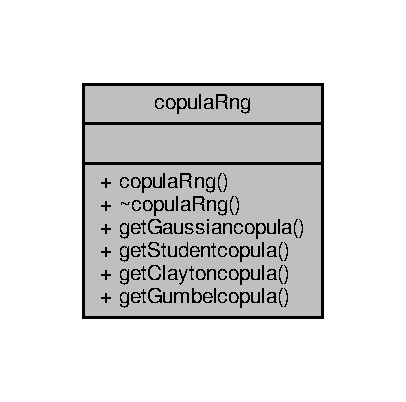
\includegraphics[width=195pt]{classcopulaRng__coll__graph}
\end{center}
\end{figure}
\subsection*{Public Member Functions}
\begin{DoxyCompactItemize}
\item 
\hyperlink{classcopulaRng_a223e069676a02b38f8bb2cafa242cf54}{copula\+Rng} (unsigned int \+\_\+d, \hyperlink{classrng}{rng} \&\+\_\+rng\+\_\+)
\item 
\hyperlink{classcopulaRng_a2adb46d54717a4c76f9a46245ee3cacc}{$\sim$copula\+Rng} ()
\item 
\hyperlink{compute__returns__eigen_8h_a1eb6a9306ef406d7975f3cbf2e247777}{Vec} \hyperlink{classcopulaRng_a1aac3848b57818708af45d7cb3bdfa9f}{get\+Gaussiancopula} (Eigen\+::\+Matrix\+Xd C)
\item 
\hyperlink{compute__returns__eigen_8h_a1eb6a9306ef406d7975f3cbf2e247777}{Vec} \hyperlink{classcopulaRng_a6d06b353f8c4eec06084919c254a8a40}{get\+Studentcopula} (Eigen\+::\+Matrix\+Xd C, double v)
\item 
\hyperlink{compute__returns__eigen_8h_a1eb6a9306ef406d7975f3cbf2e247777}{Vec} \hyperlink{classcopulaRng_a8da7d9a900602dfbb03fff3a627a8763}{get\+Claytoncopula} (double gamma)
\item 
\hyperlink{compute__returns__eigen_8h_a1eb6a9306ef406d7975f3cbf2e247777}{Vec} \hyperlink{classcopulaRng_a7806378704438e24b852da445f999b08}{get\+Gumbelcopula} (double gamma)
\end{DoxyCompactItemize}


\subsection{Detailed Description}
Simulate d variables via copula of choice

Gaussian, Student, Clayton, Gumbel 

\subsection{Constructor \& Destructor Documentation}
\hypertarget{classcopulaRng_a223e069676a02b38f8bb2cafa242cf54}{}\label{classcopulaRng_a223e069676a02b38f8bb2cafa242cf54} 
\index{copula\+Rng@{copula\+Rng}!copula\+Rng@{copula\+Rng}}
\index{copula\+Rng@{copula\+Rng}!copula\+Rng@{copula\+Rng}}
\subsubsection{\texorpdfstring{copula\+Rng()}{copulaRng()}}
{\footnotesize\ttfamily copula\+Rng\+::copula\+Rng (\begin{DoxyParamCaption}\item[{unsigned int}]{\+\_\+d,  }\item[{\hyperlink{classrng}{rng} \&}]{\+\_\+rng\+\_\+ }\end{DoxyParamCaption})}

\hypertarget{classcopulaRng_a2adb46d54717a4c76f9a46245ee3cacc}{}\label{classcopulaRng_a2adb46d54717a4c76f9a46245ee3cacc} 
\index{copula\+Rng@{copula\+Rng}!````~copula\+Rng@{$\sim$copula\+Rng}}
\index{````~copula\+Rng@{$\sim$copula\+Rng}!copula\+Rng@{copula\+Rng}}
\subsubsection{\texorpdfstring{$\sim$copula\+Rng()}{~copulaRng()}}
{\footnotesize\ttfamily copula\+Rng\+::$\sim$copula\+Rng (\begin{DoxyParamCaption}{ }\end{DoxyParamCaption})\hspace{0.3cm}{\ttfamily [inline]}}



\subsection{Member Function Documentation}
\hypertarget{classcopulaRng_a8da7d9a900602dfbb03fff3a627a8763}{}\label{classcopulaRng_a8da7d9a900602dfbb03fff3a627a8763} 
\index{copula\+Rng@{copula\+Rng}!get\+Claytoncopula@{get\+Claytoncopula}}
\index{get\+Claytoncopula@{get\+Claytoncopula}!copula\+Rng@{copula\+Rng}}
\subsubsection{\texorpdfstring{get\+Claytoncopula()}{getClaytoncopula()}}
{\footnotesize\ttfamily \hyperlink{compute__returns__eigen_8h_a1eb6a9306ef406d7975f3cbf2e247777}{Vec} copula\+Rng\+::get\+Claytoncopula (\begin{DoxyParamCaption}\item[{double}]{gamma }\end{DoxyParamCaption})}

Clayon copula. More emphasis on the left tail of the distribution


\begin{DoxyParams}{Parameters}
{\em gamma} & $\gamma$ \\
\hline
\end{DoxyParams}
\begin{DoxyReturn}{Returns}
vector of d-\/size draws from $U(0,1)$ 
\end{DoxyReturn}
\hypertarget{classcopulaRng_a1aac3848b57818708af45d7cb3bdfa9f}{}\label{classcopulaRng_a1aac3848b57818708af45d7cb3bdfa9f} 
\index{copula\+Rng@{copula\+Rng}!get\+Gaussiancopula@{get\+Gaussiancopula}}
\index{get\+Gaussiancopula@{get\+Gaussiancopula}!copula\+Rng@{copula\+Rng}}
\subsubsection{\texorpdfstring{get\+Gaussiancopula()}{getGaussiancopula()}}
{\footnotesize\ttfamily \hyperlink{compute__returns__eigen_8h_a1eb6a9306ef406d7975f3cbf2e247777}{Vec} copula\+Rng\+::get\+Gaussiancopula (\begin{DoxyParamCaption}\item[{Eigen\+::\+Matrix\+Xd}]{C }\end{DoxyParamCaption})}

Gaussian copula


\begin{DoxyParams}{Parameters}
{\em \+\_\+C} & correlation matrix \\
\hline
\end{DoxyParams}
\begin{DoxyReturn}{Returns}
vector of d-\/size draws from $U(0,1)$ 
\end{DoxyReturn}
\hypertarget{classcopulaRng_a7806378704438e24b852da445f999b08}{}\label{classcopulaRng_a7806378704438e24b852da445f999b08} 
\index{copula\+Rng@{copula\+Rng}!get\+Gumbelcopula@{get\+Gumbelcopula}}
\index{get\+Gumbelcopula@{get\+Gumbelcopula}!copula\+Rng@{copula\+Rng}}
\subsubsection{\texorpdfstring{get\+Gumbelcopula()}{getGumbelcopula()}}
{\footnotesize\ttfamily \hyperlink{compute__returns__eigen_8h_a1eb6a9306ef406d7975f3cbf2e247777}{Vec} copula\+Rng\+::get\+Gumbelcopula (\begin{DoxyParamCaption}\item[{double}]{gamma }\end{DoxyParamCaption})}

Gumbel copula. More emphasis on the right tail of the distribution


\begin{DoxyParams}{Parameters}
{\em gamma} & $\gamma$ \\
\hline
\end{DoxyParams}
\begin{DoxyReturn}{Returns}
vector of d-\/size draws from $U(0,1)$ 
\end{DoxyReturn}
\hypertarget{classcopulaRng_a6d06b353f8c4eec06084919c254a8a40}{}\label{classcopulaRng_a6d06b353f8c4eec06084919c254a8a40} 
\index{copula\+Rng@{copula\+Rng}!get\+Studentcopula@{get\+Studentcopula}}
\index{get\+Studentcopula@{get\+Studentcopula}!copula\+Rng@{copula\+Rng}}
\subsubsection{\texorpdfstring{get\+Studentcopula()}{getStudentcopula()}}
{\footnotesize\ttfamily \hyperlink{compute__returns__eigen_8h_a1eb6a9306ef406d7975f3cbf2e247777}{Vec} copula\+Rng\+::get\+Studentcopula (\begin{DoxyParamCaption}\item[{Eigen\+::\+Matrix\+Xd}]{C,  }\item[{double}]{v }\end{DoxyParamCaption})}

Student\textquotesingle{}s t copula


\begin{DoxyParams}{Parameters}
{\em \+\_\+C} & correlation matrix \\
\hline
{\em v} & $\nu$ degree of freedom \\
\hline
\end{DoxyParams}
\begin{DoxyReturn}{Returns}
vector of d-\/size draws from $U(0,1)$ 
\end{DoxyReturn}


The documentation for this class was generated from the following file\+:\begin{DoxyCompactItemize}
\item 
\hyperlink{rng_8h}{rng.\+h}\end{DoxyCompactItemize}

\hypertarget{classDeltaOne}{}\section{Delta\+One Class Reference}
\label{classDeltaOne}\index{Delta\+One@{Delta\+One}}


Sensitivity one for one. FX, index, commodity prices.  




{\ttfamily \#include $<$instrument.\+h$>$}



Inheritance diagram for Delta\+One\+:
\nopagebreak
\begin{figure}[H]
\begin{center}
\leavevmode
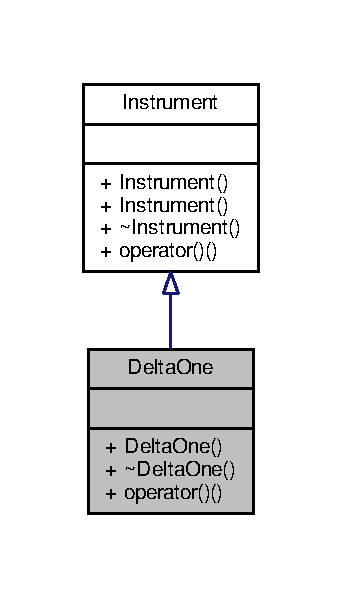
\includegraphics[width=164pt]{classDeltaOne__inherit__graph}
\end{center}
\end{figure}


Collaboration diagram for Delta\+One\+:
\nopagebreak
\begin{figure}[H]
\begin{center}
\leavevmode
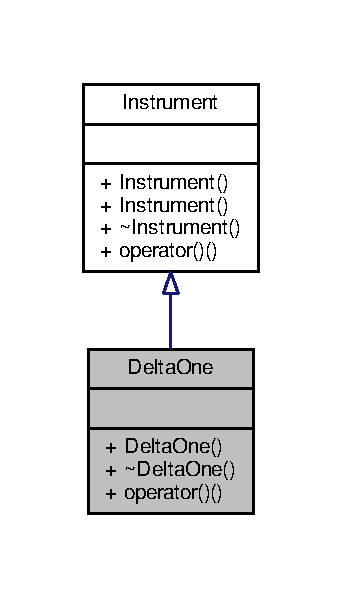
\includegraphics[width=164pt]{classDeltaOne__coll__graph}
\end{center}
\end{figure}
\subsection*{Public Member Functions}
\begin{DoxyCompactItemize}
\item 
\hyperlink{classDeltaOne_a4f3965ead9df38e2cf4a3934b1ea468e}{Delta\+One} ()
\item 
virtual \hyperlink{classDeltaOne_af954cd06f4df10cdc02244aeda02e7c5}{$\sim$\+Delta\+One} ()
\item 
double \hyperlink{classDeltaOne_a8dd4b5243412ab399b07c1128262f570}{operator()} (double rtn) const
\begin{DoxyCompactList}\small\item\em Compute an approximation on P\&L of instrument following shock. \end{DoxyCompactList}\end{DoxyCompactItemize}


\subsection{Detailed Description}
Sensitivity one for one. FX, index, commodity prices. 

\subsection{Constructor \& Destructor Documentation}
\hypertarget{classDeltaOne_a4f3965ead9df38e2cf4a3934b1ea468e}{}\label{classDeltaOne_a4f3965ead9df38e2cf4a3934b1ea468e} 
\index{Delta\+One@{Delta\+One}!Delta\+One@{Delta\+One}}
\index{Delta\+One@{Delta\+One}!Delta\+One@{Delta\+One}}
\subsubsection{\texorpdfstring{Delta\+One()}{DeltaOne()}}
{\footnotesize\ttfamily Delta\+One\+::\+Delta\+One (\begin{DoxyParamCaption}{ }\end{DoxyParamCaption})}

\hypertarget{classDeltaOne_af954cd06f4df10cdc02244aeda02e7c5}{}\label{classDeltaOne_af954cd06f4df10cdc02244aeda02e7c5} 
\index{Delta\+One@{Delta\+One}!````~Delta\+One@{$\sim$\+Delta\+One}}
\index{````~Delta\+One@{$\sim$\+Delta\+One}!Delta\+One@{Delta\+One}}
\subsubsection{\texorpdfstring{$\sim$\+Delta\+One()}{~DeltaOne()}}
{\footnotesize\ttfamily virtual Delta\+One\+::$\sim$\+Delta\+One (\begin{DoxyParamCaption}{ }\end{DoxyParamCaption})\hspace{0.3cm}{\ttfamily [inline]}, {\ttfamily [virtual]}}



\subsection{Member Function Documentation}
\hypertarget{classDeltaOne_a8dd4b5243412ab399b07c1128262f570}{}\label{classDeltaOne_a8dd4b5243412ab399b07c1128262f570} 
\index{Delta\+One@{Delta\+One}!operator()@{operator()}}
\index{operator()@{operator()}!Delta\+One@{Delta\+One}}
\subsubsection{\texorpdfstring{operator()()}{operator()()}}
{\footnotesize\ttfamily double Delta\+One\+::operator() (\begin{DoxyParamCaption}\item[{double}]{rtn }\end{DoxyParamCaption}) const\hspace{0.3cm}{\ttfamily [virtual]}}



Compute an approximation on P\&L of instrument following shock. 



Implements \hyperlink{classInstrument_a33b6faccaeb494858dee5c547de897b6}{Instrument}.



The documentation for this class was generated from the following file\+:\begin{DoxyCompactItemize}
\item 
\hyperlink{instrument_8h}{instrument.\+h}\end{DoxyCompactItemize}

\hypertarget{classDerivatives}{}\section{Derivatives Class Reference}
\label{classDerivatives}\index{Derivatives@{Derivatives}}


{\ttfamily \#include $<$instrument.\+h$>$}



Inheritance diagram for Derivatives\+:
\nopagebreak
\begin{figure}[H]
\begin{center}
\leavevmode
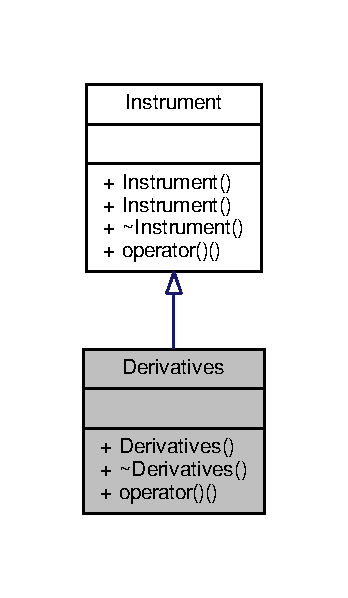
\includegraphics[width=167pt]{classDerivatives__inherit__graph}
\end{center}
\end{figure}


Collaboration diagram for Derivatives\+:
\nopagebreak
\begin{figure}[H]
\begin{center}
\leavevmode
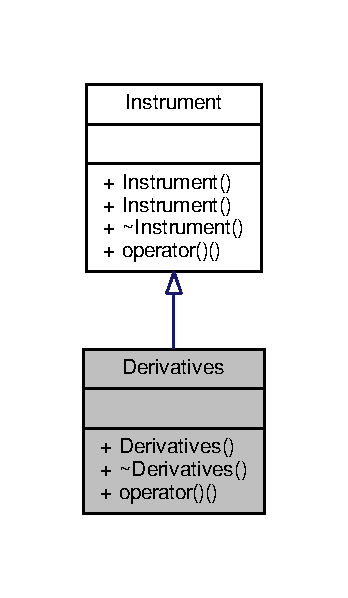
\includegraphics[width=167pt]{classDerivatives__coll__graph}
\end{center}
\end{figure}
\subsection*{Public Member Functions}
\begin{DoxyCompactItemize}
\item 
\hyperlink{classDerivatives_ab78961446af3fcbfd6cdb0f89ef0eecf}{Derivatives} (double \+\_\+delta, double \+\_\+gamma)
\item 
virtual \hyperlink{classDerivatives_a5766623ccaf59ea949410e456a464b73}{$\sim$\+Derivatives} ()
\item 
double \hyperlink{classDerivatives_a765ecae139ee81fb5143a20462211623}{operator()} (double rtn) const
\begin{DoxyCompactList}\small\item\em Compute an approximation on P\&L of instrument following shock. \end{DoxyCompactList}\end{DoxyCompactItemize}


\subsection{Constructor \& Destructor Documentation}
\hypertarget{classDerivatives_ab78961446af3fcbfd6cdb0f89ef0eecf}{}\label{classDerivatives_ab78961446af3fcbfd6cdb0f89ef0eecf} 
\index{Derivatives@{Derivatives}!Derivatives@{Derivatives}}
\index{Derivatives@{Derivatives}!Derivatives@{Derivatives}}
\subsubsection{\texorpdfstring{Derivatives()}{Derivatives()}}
{\footnotesize\ttfamily Derivatives\+::\+Derivatives (\begin{DoxyParamCaption}\item[{double}]{\+\_\+delta,  }\item[{double}]{\+\_\+gamma }\end{DoxyParamCaption})}

\hypertarget{classDerivatives_a5766623ccaf59ea949410e456a464b73}{}\label{classDerivatives_a5766623ccaf59ea949410e456a464b73} 
\index{Derivatives@{Derivatives}!````~Derivatives@{$\sim$\+Derivatives}}
\index{````~Derivatives@{$\sim$\+Derivatives}!Derivatives@{Derivatives}}
\subsubsection{\texorpdfstring{$\sim$\+Derivatives()}{~Derivatives()}}
{\footnotesize\ttfamily virtual Derivatives\+::$\sim$\+Derivatives (\begin{DoxyParamCaption}{ }\end{DoxyParamCaption})\hspace{0.3cm}{\ttfamily [inline]}, {\ttfamily [virtual]}}



\subsection{Member Function Documentation}
\hypertarget{classDerivatives_a765ecae139ee81fb5143a20462211623}{}\label{classDerivatives_a765ecae139ee81fb5143a20462211623} 
\index{Derivatives@{Derivatives}!operator()@{operator()}}
\index{operator()@{operator()}!Derivatives@{Derivatives}}
\subsubsection{\texorpdfstring{operator()()}{operator()()}}
{\footnotesize\ttfamily double Derivatives\+::operator() (\begin{DoxyParamCaption}\item[{double}]{rtn }\end{DoxyParamCaption}) const\hspace{0.3cm}{\ttfamily [virtual]}}



Compute an approximation on P\&L of instrument following shock. 



Implements \hyperlink{classInstrument_a33b6faccaeb494858dee5c547de897b6}{Instrument}.



The documentation for this class was generated from the following file\+:\begin{DoxyCompactItemize}
\item 
\hyperlink{instrument_8h}{instrument.\+h}\end{DoxyCompactItemize}

\hypertarget{classEquity}{}\section{Equity Class Reference}
\label{classEquity}\index{Equity@{Equity}}


{\ttfamily \#include $<$instrument.\+h$>$}



Inheritance diagram for Equity\+:
\nopagebreak
\begin{figure}[H]
\begin{center}
\leavevmode
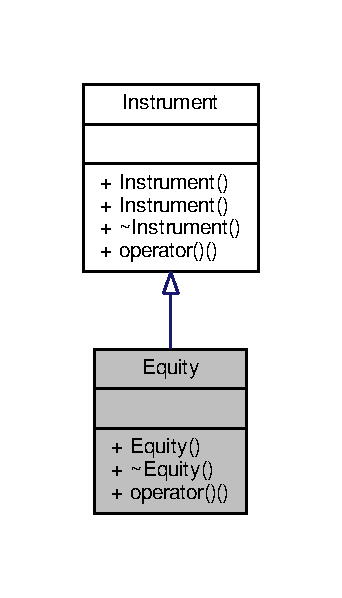
\includegraphics[width=164pt]{classEquity__inherit__graph}
\end{center}
\end{figure}


Collaboration diagram for Equity\+:
\nopagebreak
\begin{figure}[H]
\begin{center}
\leavevmode
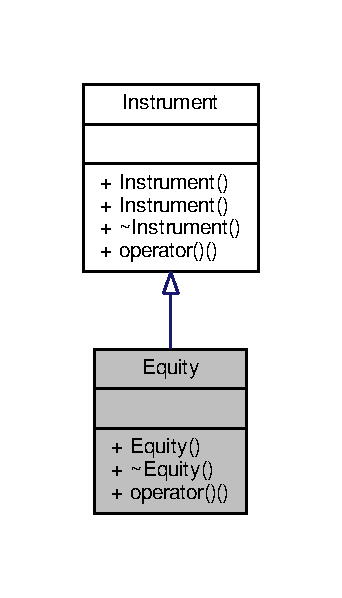
\includegraphics[width=164pt]{classEquity__coll__graph}
\end{center}
\end{figure}
\subsection*{Public Member Functions}
\begin{DoxyCompactItemize}
\item 
\hyperlink{classEquity_a3560f0e47c12a99611a97072e0a3deea}{Equity} (double \+\_\+beta=1.)
\item 
virtual \hyperlink{classEquity_af3ff4776470bcc86d607577fa947bb5b}{$\sim$\+Equity} ()
\item 
double \hyperlink{classEquity_a2844b7fa3dd164ce216909d1fe958c9f}{operator()} (double rtn) const
\begin{DoxyCompactList}\small\item\em Compute an approximation on P\&L of instrument following shock. \end{DoxyCompactList}\end{DoxyCompactItemize}


\subsection{Constructor \& Destructor Documentation}
\hypertarget{classEquity_a3560f0e47c12a99611a97072e0a3deea}{}\label{classEquity_a3560f0e47c12a99611a97072e0a3deea} 
\index{Equity@{Equity}!Equity@{Equity}}
\index{Equity@{Equity}!Equity@{Equity}}
\subsubsection{\texorpdfstring{Equity()}{Equity()}}
{\footnotesize\ttfamily Equity\+::\+Equity (\begin{DoxyParamCaption}\item[{double}]{\+\_\+beta = {\ttfamily 1.} }\end{DoxyParamCaption})}

\hypertarget{classEquity_af3ff4776470bcc86d607577fa947bb5b}{}\label{classEquity_af3ff4776470bcc86d607577fa947bb5b} 
\index{Equity@{Equity}!````~Equity@{$\sim$\+Equity}}
\index{````~Equity@{$\sim$\+Equity}!Equity@{Equity}}
\subsubsection{\texorpdfstring{$\sim$\+Equity()}{~Equity()}}
{\footnotesize\ttfamily virtual Equity\+::$\sim$\+Equity (\begin{DoxyParamCaption}{ }\end{DoxyParamCaption})\hspace{0.3cm}{\ttfamily [inline]}, {\ttfamily [virtual]}}



\subsection{Member Function Documentation}
\hypertarget{classEquity_a2844b7fa3dd164ce216909d1fe958c9f}{}\label{classEquity_a2844b7fa3dd164ce216909d1fe958c9f} 
\index{Equity@{Equity}!operator()@{operator()}}
\index{operator()@{operator()}!Equity@{Equity}}
\subsubsection{\texorpdfstring{operator()()}{operator()()}}
{\footnotesize\ttfamily double Equity\+::operator() (\begin{DoxyParamCaption}\item[{double}]{rtn }\end{DoxyParamCaption}) const\hspace{0.3cm}{\ttfamily [virtual]}}



Compute an approximation on P\&L of instrument following shock. 



Implements \hyperlink{classInstrument_a33b6faccaeb494858dee5c547de897b6}{Instrument}.



The documentation for this class was generated from the following file\+:\begin{DoxyCompactItemize}
\item 
\hyperlink{instrument_8h}{instrument.\+h}\end{DoxyCompactItemize}

\hypertarget{classExtremeValueVaR}{}\section{Extreme\+Value\+VaR Class Reference}
\label{classExtremeValueVaR}\index{Extreme\+Value\+VaR@{Extreme\+Value\+VaR}}


{\ttfamily \#include $<$var\+\_\+model.\+h$>$}



Inheritance diagram for Extreme\+Value\+VaR\+:
\nopagebreak
\begin{figure}[H]
\begin{center}
\leavevmode
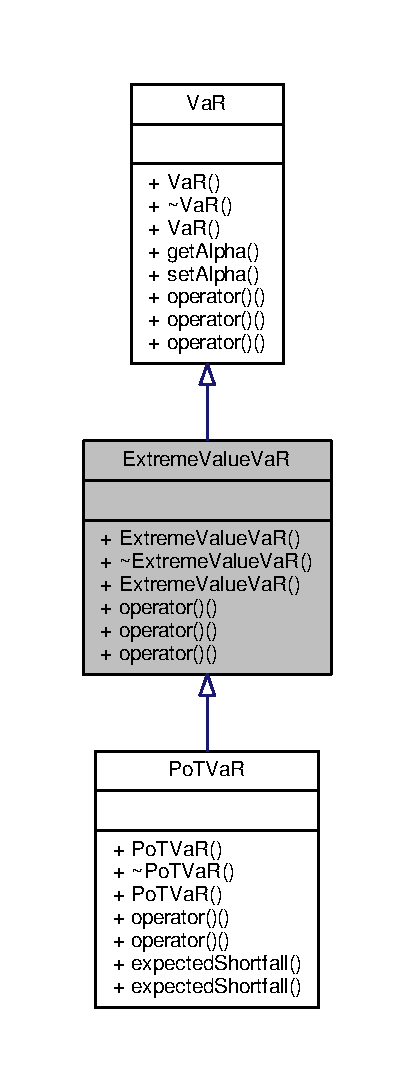
\includegraphics[width=199pt]{classExtremeValueVaR__inherit__graph}
\end{center}
\end{figure}


Collaboration diagram for Extreme\+Value\+VaR\+:
\nopagebreak
\begin{figure}[H]
\begin{center}
\leavevmode
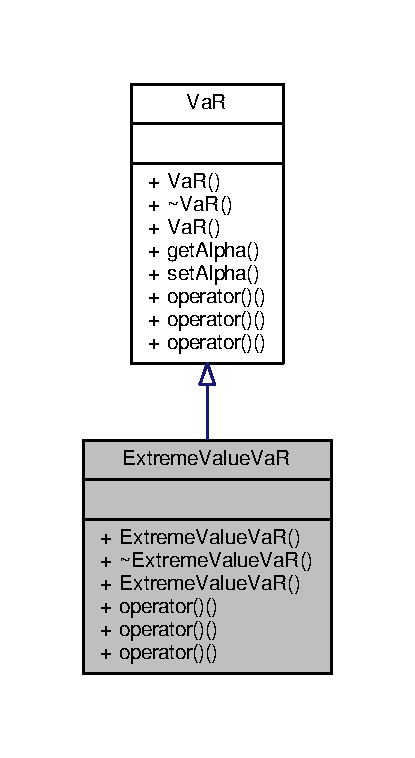
\includegraphics[width=199pt]{classExtremeValueVaR__coll__graph}
\end{center}
\end{figure}
\subsection*{Public Member Functions}
\begin{DoxyCompactItemize}
\item 
\hyperlink{classExtremeValueVaR_a0a85df72f4cd3d4e18b60e777e593c01}{Extreme\+Value\+VaR} (double \+\_\+alpha=.\+05)
\item 
virtual \hyperlink{classExtremeValueVaR_a5079f1cf38bb19547f7d68695cf5e881}{$\sim$\+Extreme\+Value\+VaR} ()
\item 
\hyperlink{classExtremeValueVaR_a1c75fd9d6ec397b4b1ebc32225c4c41a}{Extreme\+Value\+VaR} (const \hyperlink{classExtremeValueVaR}{Extreme\+Value\+VaR} \&other)
\item 
virtual double \hyperlink{classExtremeValueVaR_ad6d31417001a3ee1b75592806d21ae8b}{operator()} (double \+\_\+mean\+Return, double \+\_\+sigmatminus1, double \+\_\+returnt) const
\item 
double \hyperlink{classExtremeValueVaR_a8dfe4d515f7e4d0260b3ac87c1a52b5f}{operator()} (double \+\_\+mean\+Return, const \hyperlink{compute__returns__eigen_8h_a1eb6a9306ef406d7975f3cbf2e247777}{Vec} \&returns) const
\item 
virtual double \hyperlink{classExtremeValueVaR_a3be021ee0faa2285bcb6be19815e3dc7}{operator()} (const \hyperlink{compute__returns__eigen_8h_a1eb6a9306ef406d7975f3cbf2e247777}{Vec} \&returns) const =0
\end{DoxyCompactItemize}


\subsection{Constructor \& Destructor Documentation}
\hypertarget{classExtremeValueVaR_a0a85df72f4cd3d4e18b60e777e593c01}{}\label{classExtremeValueVaR_a0a85df72f4cd3d4e18b60e777e593c01} 
\index{Extreme\+Value\+VaR@{Extreme\+Value\+VaR}!Extreme\+Value\+VaR@{Extreme\+Value\+VaR}}
\index{Extreme\+Value\+VaR@{Extreme\+Value\+VaR}!Extreme\+Value\+VaR@{Extreme\+Value\+VaR}}
\subsubsection{\texorpdfstring{Extreme\+Value\+Va\+R()}{ExtremeValueVaR()}\hspace{0.1cm}{\footnotesize\ttfamily [1/2]}}
{\footnotesize\ttfamily Extreme\+Value\+Va\+R\+::\+Extreme\+Value\+VaR (\begin{DoxyParamCaption}\item[{double}]{\+\_\+alpha = {\ttfamily .05} }\end{DoxyParamCaption})}

\hypertarget{classExtremeValueVaR_a5079f1cf38bb19547f7d68695cf5e881}{}\label{classExtremeValueVaR_a5079f1cf38bb19547f7d68695cf5e881} 
\index{Extreme\+Value\+VaR@{Extreme\+Value\+VaR}!````~Extreme\+Value\+VaR@{$\sim$\+Extreme\+Value\+VaR}}
\index{````~Extreme\+Value\+VaR@{$\sim$\+Extreme\+Value\+VaR}!Extreme\+Value\+VaR@{Extreme\+Value\+VaR}}
\subsubsection{\texorpdfstring{$\sim$\+Extreme\+Value\+Va\+R()}{~ExtremeValueVaR()}}
{\footnotesize\ttfamily virtual Extreme\+Value\+Va\+R\+::$\sim$\+Extreme\+Value\+VaR (\begin{DoxyParamCaption}{ }\end{DoxyParamCaption})\hspace{0.3cm}{\ttfamily [inline]}, {\ttfamily [virtual]}}

\hypertarget{classExtremeValueVaR_a1c75fd9d6ec397b4b1ebc32225c4c41a}{}\label{classExtremeValueVaR_a1c75fd9d6ec397b4b1ebc32225c4c41a} 
\index{Extreme\+Value\+VaR@{Extreme\+Value\+VaR}!Extreme\+Value\+VaR@{Extreme\+Value\+VaR}}
\index{Extreme\+Value\+VaR@{Extreme\+Value\+VaR}!Extreme\+Value\+VaR@{Extreme\+Value\+VaR}}
\subsubsection{\texorpdfstring{Extreme\+Value\+Va\+R()}{ExtremeValueVaR()}\hspace{0.1cm}{\footnotesize\ttfamily [2/2]}}
{\footnotesize\ttfamily Extreme\+Value\+Va\+R\+::\+Extreme\+Value\+VaR (\begin{DoxyParamCaption}\item[{const \hyperlink{classExtremeValueVaR}{Extreme\+Value\+VaR} \&}]{other }\end{DoxyParamCaption})}



\subsection{Member Function Documentation}
\hypertarget{classExtremeValueVaR_ad6d31417001a3ee1b75592806d21ae8b}{}\label{classExtremeValueVaR_ad6d31417001a3ee1b75592806d21ae8b} 
\index{Extreme\+Value\+VaR@{Extreme\+Value\+VaR}!operator()@{operator()}}
\index{operator()@{operator()}!Extreme\+Value\+VaR@{Extreme\+Value\+VaR}}
\subsubsection{\texorpdfstring{operator()()}{operator()()}\hspace{0.1cm}{\footnotesize\ttfamily [1/3]}}
{\footnotesize\ttfamily virtual double Extreme\+Value\+Va\+R\+::operator() (\begin{DoxyParamCaption}\item[{double}]{\+\_\+mean\+Return,  }\item[{double}]{\+\_\+sigmatminus1,  }\item[{double}]{\+\_\+returnt }\end{DoxyParamCaption}) const\hspace{0.3cm}{\ttfamily [inline]}, {\ttfamily [virtual]}}



Implements \hyperlink{classVaR_a28e1a1be9e386ed4e8503e54db4033bd}{VaR}.

\hypertarget{classExtremeValueVaR_a8dfe4d515f7e4d0260b3ac87c1a52b5f}{}\label{classExtremeValueVaR_a8dfe4d515f7e4d0260b3ac87c1a52b5f} 
\index{Extreme\+Value\+VaR@{Extreme\+Value\+VaR}!operator()@{operator()}}
\index{operator()@{operator()}!Extreme\+Value\+VaR@{Extreme\+Value\+VaR}}
\subsubsection{\texorpdfstring{operator()()}{operator()()}\hspace{0.1cm}{\footnotesize\ttfamily [2/3]}}
{\footnotesize\ttfamily double Extreme\+Value\+Va\+R\+::operator() (\begin{DoxyParamCaption}\item[{double}]{\+\_\+mean\+Return,  }\item[{const \hyperlink{compute__returns__eigen_8h_a1eb6a9306ef406d7975f3cbf2e247777}{Vec} \&}]{returns }\end{DoxyParamCaption}) const\hspace{0.3cm}{\ttfamily [inline]}, {\ttfamily [virtual]}}



Implements \hyperlink{classVaR_a31cb62626488715a9133679feaba31e5}{VaR}.

\hypertarget{classExtremeValueVaR_a3be021ee0faa2285bcb6be19815e3dc7}{}\label{classExtremeValueVaR_a3be021ee0faa2285bcb6be19815e3dc7} 
\index{Extreme\+Value\+VaR@{Extreme\+Value\+VaR}!operator()@{operator()}}
\index{operator()@{operator()}!Extreme\+Value\+VaR@{Extreme\+Value\+VaR}}
\subsubsection{\texorpdfstring{operator()()}{operator()()}\hspace{0.1cm}{\footnotesize\ttfamily [3/3]}}
{\footnotesize\ttfamily virtual double Extreme\+Value\+Va\+R\+::operator() (\begin{DoxyParamCaption}\item[{const \hyperlink{compute__returns__eigen_8h_a1eb6a9306ef406d7975f3cbf2e247777}{Vec} \&}]{returns }\end{DoxyParamCaption}) const\hspace{0.3cm}{\ttfamily [pure virtual]}}



Implements \hyperlink{classVaR_a1bd868d9953bfaeb49f5bf7d16986631}{VaR}.



Implemented in \hyperlink{classPoTVaR_a3360bbbeceae9bbd0c721e48586bf38c}{Po\+T\+VaR}.



The documentation for this class was generated from the following file\+:\begin{DoxyCompactItemize}
\item 
\hyperlink{var__model_8h}{var\+\_\+model.\+h}\end{DoxyCompactItemize}

\hypertarget{classFI}{}\section{FI Class Reference}
\label{classFI}\index{FI@{FI}}


{\ttfamily \#include $<$instrument.\+h$>$}



Inheritance diagram for FI\+:
\nopagebreak
\begin{figure}[H]
\begin{center}
\leavevmode
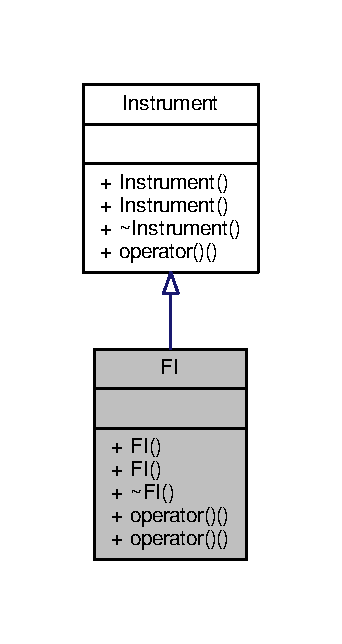
\includegraphics[width=164pt]{classFI__inherit__graph}
\end{center}
\end{figure}


Collaboration diagram for FI\+:
\nopagebreak
\begin{figure}[H]
\begin{center}
\leavevmode
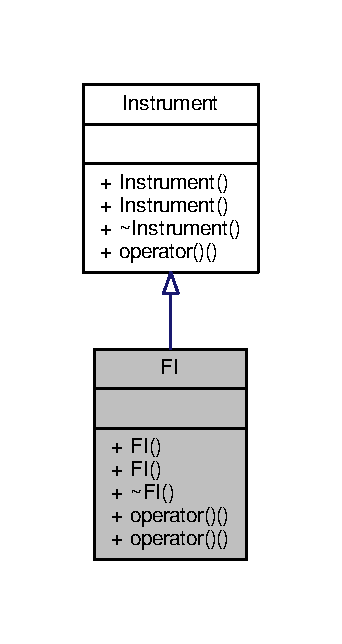
\includegraphics[width=164pt]{classFI__coll__graph}
\end{center}
\end{figure}
\subsection*{Public Member Functions}
\begin{DoxyCompactItemize}
\item 
\hyperlink{classFI_a8caa07473802c6c7dd10cc1c98af7397}{FI} (double \+\_\+duration, double \+\_\+convexity=0., \hyperlink{instrument_8h_aeef2cd5bd2753709d5c6348c32cbdaa0}{duration\+Type} \+\_\+dt=\hyperlink{instrument_8h_aeef2cd5bd2753709d5c6348c32cbdaa0a22e2e72997ac4289587cadae38cc561e}{dc})
\item 
\hyperlink{classFI_a52951d4aeccbe628a59b65968713c85f}{FI} (\hyperlink{compute__returns__eigen_8h_a1eb6a9306ef406d7975f3cbf2e247777}{Vec} \&\+\_\+duration)
\item 
virtual \hyperlink{classFI_a856ac31d9840ae7cd9eeba9482832f8a}{$\sim$\+FI} ()
\item 
double \hyperlink{classFI_a99ad4380e8178d7fd304597622a2c05c}{operator()} (double rtn) const
\begin{DoxyCompactList}\small\item\em Compute an approximation on P\&L of instrument following shock. \end{DoxyCompactList}\item 
double \hyperlink{classFI_ab50033a007000c4b4c65a5a5bc08433d}{operator()} (const \hyperlink{compute__returns__eigen_8h_a1eb6a9306ef406d7975f3cbf2e247777}{Vec} \&rtns) const
\end{DoxyCompactItemize}


\subsection{Constructor \& Destructor Documentation}
\hypertarget{classFI_a8caa07473802c6c7dd10cc1c98af7397}{}\label{classFI_a8caa07473802c6c7dd10cc1c98af7397} 
\index{FI@{FI}!FI@{FI}}
\index{FI@{FI}!FI@{FI}}
\subsubsection{\texorpdfstring{F\+I()}{FI()}\hspace{0.1cm}{\footnotesize\ttfamily [1/2]}}
{\footnotesize\ttfamily F\+I\+::\+FI (\begin{DoxyParamCaption}\item[{double}]{\+\_\+duration,  }\item[{double}]{\+\_\+convexity = {\ttfamily 0.},  }\item[{\hyperlink{instrument_8h_aeef2cd5bd2753709d5c6348c32cbdaa0}{duration\+Type}}]{\+\_\+dt = {\ttfamily \hyperlink{instrument_8h_aeef2cd5bd2753709d5c6348c32cbdaa0a22e2e72997ac4289587cadae38cc561e}{dc}} }\end{DoxyParamCaption})}

\hypertarget{classFI_a52951d4aeccbe628a59b65968713c85f}{}\label{classFI_a52951d4aeccbe628a59b65968713c85f} 
\index{FI@{FI}!FI@{FI}}
\index{FI@{FI}!FI@{FI}}
\subsubsection{\texorpdfstring{F\+I()}{FI()}\hspace{0.1cm}{\footnotesize\ttfamily [2/2]}}
{\footnotesize\ttfamily F\+I\+::\+FI (\begin{DoxyParamCaption}\item[{\hyperlink{compute__returns__eigen_8h_a1eb6a9306ef406d7975f3cbf2e247777}{Vec} \&}]{\+\_\+duration }\end{DoxyParamCaption})}

\hypertarget{classFI_a856ac31d9840ae7cd9eeba9482832f8a}{}\label{classFI_a856ac31d9840ae7cd9eeba9482832f8a} 
\index{FI@{FI}!````~FI@{$\sim$\+FI}}
\index{````~FI@{$\sim$\+FI}!FI@{FI}}
\subsubsection{\texorpdfstring{$\sim$\+F\+I()}{~FI()}}
{\footnotesize\ttfamily virtual F\+I\+::$\sim$\+FI (\begin{DoxyParamCaption}{ }\end{DoxyParamCaption})\hspace{0.3cm}{\ttfamily [inline]}, {\ttfamily [virtual]}}



\subsection{Member Function Documentation}
\hypertarget{classFI_a99ad4380e8178d7fd304597622a2c05c}{}\label{classFI_a99ad4380e8178d7fd304597622a2c05c} 
\index{FI@{FI}!operator()@{operator()}}
\index{operator()@{operator()}!FI@{FI}}
\subsubsection{\texorpdfstring{operator()()}{operator()()}\hspace{0.1cm}{\footnotesize\ttfamily [1/2]}}
{\footnotesize\ttfamily double F\+I\+::operator() (\begin{DoxyParamCaption}\item[{double}]{rtn }\end{DoxyParamCaption}) const\hspace{0.3cm}{\ttfamily [virtual]}}



Compute an approximation on P\&L of instrument following shock. 



Implements \hyperlink{classInstrument_a33b6faccaeb494858dee5c547de897b6}{Instrument}.

\hypertarget{classFI_ab50033a007000c4b4c65a5a5bc08433d}{}\label{classFI_ab50033a007000c4b4c65a5a5bc08433d} 
\index{FI@{FI}!operator()@{operator()}}
\index{operator()@{operator()}!FI@{FI}}
\subsubsection{\texorpdfstring{operator()()}{operator()()}\hspace{0.1cm}{\footnotesize\ttfamily [2/2]}}
{\footnotesize\ttfamily double F\+I\+::operator() (\begin{DoxyParamCaption}\item[{const \hyperlink{compute__returns__eigen_8h_a1eb6a9306ef406d7975f3cbf2e247777}{Vec} \&}]{rtns }\end{DoxyParamCaption}) const}



The documentation for this class was generated from the following file\+:\begin{DoxyCompactItemize}
\item 
\hyperlink{instrument_8h}{instrument.\+h}\end{DoxyCompactItemize}

\hypertarget{classGARCH11}{}\section{G\+A\+R\+C\+H11 Class Reference}
\label{classGARCH11}\index{G\+A\+R\+C\+H11@{G\+A\+R\+C\+H11}}


model G\+A\+R\+C\+H(1,1)  




{\ttfamily \#include $<$path.\+h$>$}



Inheritance diagram for G\+A\+R\+C\+H11\+:
\nopagebreak
\begin{figure}[H]
\begin{center}
\leavevmode
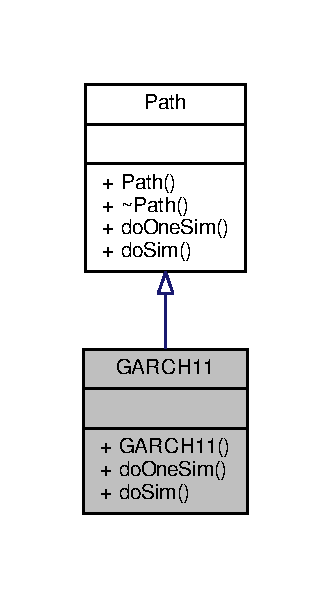
\includegraphics[width=159pt]{classGARCH11__inherit__graph}
\end{center}
\end{figure}


Collaboration diagram for G\+A\+R\+C\+H11\+:
\nopagebreak
\begin{figure}[H]
\begin{center}
\leavevmode
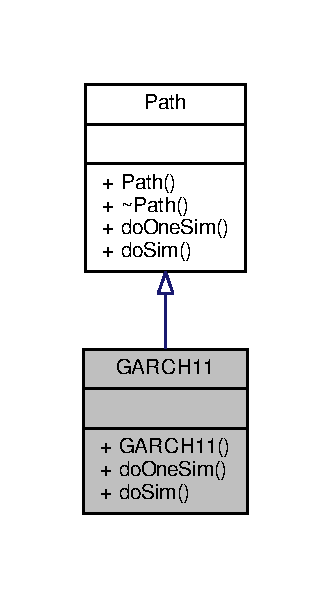
\includegraphics[width=159pt]{classGARCH11__coll__graph}
\end{center}
\end{figure}
\subsection*{Public Member Functions}
\begin{DoxyCompactItemize}
\item 
\hyperlink{classGARCH11_a7c6f1b56ce23150073f733a64f21bffc}{G\+A\+R\+C\+H11} (double \+\_\+alpha=0., double \+\_\+beta=.\+24, double \+\_\+gamma=.\+76)
\item 
virtual double \hyperlink{classGARCH11_a8f6e87b2b85a91e02416d4d02bf7b9ff}{do\+One\+Sim} (const double \&u, const double \&Sigmat, const double \&Returnt, const double \&Returntminus1=0.) const
\item 
virtual Eigen\+::\+Vector\+Xd \hyperlink{classGARCH11_a202ee361532058114cfc036c27bef601}{do\+Sim} (const \hyperlink{compute__returns__eigen_8h_a1eb6a9306ef406d7975f3cbf2e247777}{Vec} \&u, const \hyperlink{compute__returns__eigen_8h_a1eb6a9306ef406d7975f3cbf2e247777}{Vec} \&Sigmat, const \hyperlink{compute__returns__eigen_8h_a1eb6a9306ef406d7975f3cbf2e247777}{Vec} \&Returnt) const
\begin{DoxyCompactList}\small\item\em Simultate return over whole path. \end{DoxyCompactList}\end{DoxyCompactItemize}


\subsection{Detailed Description}
model G\+A\+R\+C\+H(1,1) 

\subsection{Constructor \& Destructor Documentation}
\hypertarget{classGARCH11_a7c6f1b56ce23150073f733a64f21bffc}{}\label{classGARCH11_a7c6f1b56ce23150073f733a64f21bffc} 
\index{G\+A\+R\+C\+H11@{G\+A\+R\+C\+H11}!G\+A\+R\+C\+H11@{G\+A\+R\+C\+H11}}
\index{G\+A\+R\+C\+H11@{G\+A\+R\+C\+H11}!G\+A\+R\+C\+H11@{G\+A\+R\+C\+H11}}
\subsubsection{\texorpdfstring{G\+A\+R\+C\+H11()}{GARCH11()}}
{\footnotesize\ttfamily G\+A\+R\+C\+H11\+::\+G\+A\+R\+C\+H11 (\begin{DoxyParamCaption}\item[{double}]{\+\_\+alpha = {\ttfamily 0.},  }\item[{double}]{\+\_\+beta = {\ttfamily .24},  }\item[{double}]{\+\_\+gamma = {\ttfamily .76} }\end{DoxyParamCaption})}


\begin{DoxyParams}{Parameters}
{\em \+\_\+alpha} & $\alpha$ alpha G\+A\+R\+CH process \\
\hline
{\em \+\_\+beta} & $\beta$ beta G\+A\+R\+CH process \\
\hline
{\em \+\_\+gamma} & $\gamma$ gamma G\+A\+R\+CH process \\
\hline
\end{DoxyParams}


\subsection{Member Function Documentation}
\hypertarget{classGARCH11_a8f6e87b2b85a91e02416d4d02bf7b9ff}{}\label{classGARCH11_a8f6e87b2b85a91e02416d4d02bf7b9ff} 
\index{G\+A\+R\+C\+H11@{G\+A\+R\+C\+H11}!do\+One\+Sim@{do\+One\+Sim}}
\index{do\+One\+Sim@{do\+One\+Sim}!G\+A\+R\+C\+H11@{G\+A\+R\+C\+H11}}
\subsubsection{\texorpdfstring{do\+One\+Sim()}{doOneSim()}}
{\footnotesize\ttfamily virtual double G\+A\+R\+C\+H11\+::do\+One\+Sim (\begin{DoxyParamCaption}\item[{const double \&}]{u,  }\item[{const double \&}]{Sigmat,  }\item[{const double \&}]{Returnt,  }\item[{const double \&}]{Returntminus1 = {\ttfamily 0.} }\end{DoxyParamCaption}) const\hspace{0.3cm}{\ttfamily [virtual]}}

Simulate return for next period under review 
\begin{DoxyParams}{Parameters}
{\em Returntminus1} & $r_{t-1}$ return previous period \\
\hline
{\em Sigmatminus1} & $\sigma_{t-1}$ vol previous period \\
\hline
{\em u} & innovation drawn sample distr. \\
\hline
{\em v} & innovation drawn sample distr. \\
\hline
\end{DoxyParams}


Implements \hyperlink{classPath_a6e75e5a329c48cafecd03a355f90b694}{Path}.

\hypertarget{classGARCH11_a202ee361532058114cfc036c27bef601}{}\label{classGARCH11_a202ee361532058114cfc036c27bef601} 
\index{G\+A\+R\+C\+H11@{G\+A\+R\+C\+H11}!do\+Sim@{do\+Sim}}
\index{do\+Sim@{do\+Sim}!G\+A\+R\+C\+H11@{G\+A\+R\+C\+H11}}
\subsubsection{\texorpdfstring{do\+Sim()}{doSim()}}
{\footnotesize\ttfamily virtual Eigen\+::\+Vector\+Xd G\+A\+R\+C\+H11\+::do\+Sim (\begin{DoxyParamCaption}\item[{const \hyperlink{compute__returns__eigen_8h_a1eb6a9306ef406d7975f3cbf2e247777}{Vec} \&}]{u,  }\item[{const \hyperlink{compute__returns__eigen_8h_a1eb6a9306ef406d7975f3cbf2e247777}{Vec} \&}]{Sigmat,  }\item[{const \hyperlink{compute__returns__eigen_8h_a1eb6a9306ef406d7975f3cbf2e247777}{Vec} \&}]{Returnt }\end{DoxyParamCaption}) const\hspace{0.3cm}{\ttfamily [virtual]}}



Simultate return over whole path. 



Implements \hyperlink{classPath_a8917612a585bce52dbd52b1b643a517a}{Path}.



The documentation for this class was generated from the following file\+:\begin{DoxyCompactItemize}
\item 
\hyperlink{path_8h}{path.\+h}\end{DoxyCompactItemize}

\hypertarget{classGarchVaR}{}\section{Garch\+VaR Class Reference}
\label{classGarchVaR}\index{Garch\+VaR@{Garch\+VaR}}


Compute G\+A\+R\+C\+H(1,1) \hyperlink{classVaR}{VaR}.  




{\ttfamily \#include $<$var\+\_\+model.\+h$>$}



Inheritance diagram for Garch\+VaR\+:
\nopagebreak
\begin{figure}[H]
\begin{center}
\leavevmode
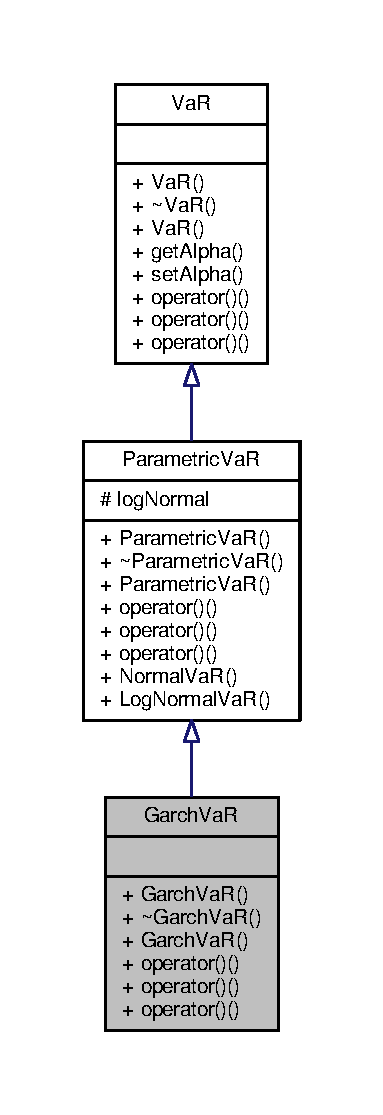
\includegraphics[width=184pt]{classGarchVaR__inherit__graph}
\end{center}
\end{figure}


Collaboration diagram for Garch\+VaR\+:
\nopagebreak
\begin{figure}[H]
\begin{center}
\leavevmode
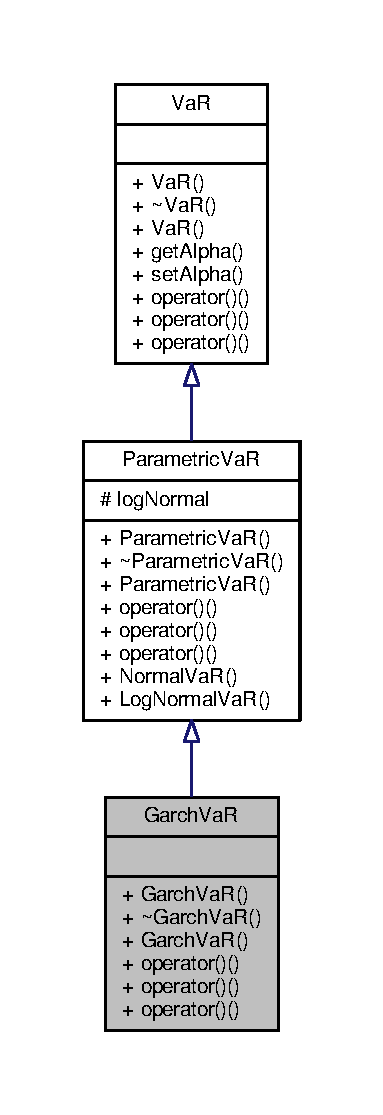
\includegraphics[width=184pt]{classGarchVaR__coll__graph}
\end{center}
\end{figure}
\subsection*{Public Member Functions}
\begin{DoxyCompactItemize}
\item 
\hyperlink{classGarchVaR_a90617aa33c7b190422bc3cfda282167b}{Garch\+VaR} (double \+\_\+alpha=.\+05, double \+\_\+a=0., double \+\_\+b=.\+74, double \+\_\+c=.\+26, bool \+\_\+log\+Normal=false)
\item 
virtual \hyperlink{classGarchVaR_aa95d7d35fad664439c72013528b6f7e1}{$\sim$\+Garch\+VaR} ()
\item 
\hyperlink{classGarchVaR_a5a8f06045676f3e8776bf49f08bea635}{Garch\+VaR} (const \hyperlink{classGarchVaR}{Garch\+VaR} \&other)
\item 
double \hyperlink{classGarchVaR_a6aec8c89e48d2b2f356669ed3300f456}{operator()} (double \+\_\+mean\+Return, double \+\_\+sigmatminus1, double \+\_\+returntminus1) const
\item 
double \hyperlink{classGarchVaR_ab7e9583566b26a64017edbbfb63f3e89}{operator()} (double \+\_\+mean\+Return, const \hyperlink{compute__returns__eigen_8h_a1eb6a9306ef406d7975f3cbf2e247777}{Vec} \&returns) const
\item 
double \hyperlink{classGarchVaR_ac6d01b6567a6d0629cd95be716677763}{operator()} (const \hyperlink{compute__returns__eigen_8h_a1eb6a9306ef406d7975f3cbf2e247777}{Vec} \&returns) const
\end{DoxyCompactItemize}
\subsection*{Additional Inherited Members}


\subsection{Detailed Description}
Compute G\+A\+R\+C\+H(1,1) \hyperlink{classVaR}{VaR}. 

\subsection{Constructor \& Destructor Documentation}
\hypertarget{classGarchVaR_a90617aa33c7b190422bc3cfda282167b}{}\label{classGarchVaR_a90617aa33c7b190422bc3cfda282167b} 
\index{Garch\+VaR@{Garch\+VaR}!Garch\+VaR@{Garch\+VaR}}
\index{Garch\+VaR@{Garch\+VaR}!Garch\+VaR@{Garch\+VaR}}
\subsubsection{\texorpdfstring{Garch\+Va\+R()}{GarchVaR()}\hspace{0.1cm}{\footnotesize\ttfamily [1/2]}}
{\footnotesize\ttfamily Garch\+Va\+R\+::\+Garch\+VaR (\begin{DoxyParamCaption}\item[{double}]{\+\_\+alpha = {\ttfamily .05},  }\item[{double}]{\+\_\+a = {\ttfamily 0.},  }\item[{double}]{\+\_\+b = {\ttfamily .74},  }\item[{double}]{\+\_\+c = {\ttfamily .26},  }\item[{bool}]{\+\_\+log\+Normal = {\ttfamily false} }\end{DoxyParamCaption})}

\hypertarget{classGarchVaR_aa95d7d35fad664439c72013528b6f7e1}{}\label{classGarchVaR_aa95d7d35fad664439c72013528b6f7e1} 
\index{Garch\+VaR@{Garch\+VaR}!````~Garch\+VaR@{$\sim$\+Garch\+VaR}}
\index{````~Garch\+VaR@{$\sim$\+Garch\+VaR}!Garch\+VaR@{Garch\+VaR}}
\subsubsection{\texorpdfstring{$\sim$\+Garch\+Va\+R()}{~GarchVaR()}}
{\footnotesize\ttfamily virtual Garch\+Va\+R\+::$\sim$\+Garch\+VaR (\begin{DoxyParamCaption}{ }\end{DoxyParamCaption})\hspace{0.3cm}{\ttfamily [inline]}, {\ttfamily [virtual]}}

\hypertarget{classGarchVaR_a5a8f06045676f3e8776bf49f08bea635}{}\label{classGarchVaR_a5a8f06045676f3e8776bf49f08bea635} 
\index{Garch\+VaR@{Garch\+VaR}!Garch\+VaR@{Garch\+VaR}}
\index{Garch\+VaR@{Garch\+VaR}!Garch\+VaR@{Garch\+VaR}}
\subsubsection{\texorpdfstring{Garch\+Va\+R()}{GarchVaR()}\hspace{0.1cm}{\footnotesize\ttfamily [2/2]}}
{\footnotesize\ttfamily Garch\+Va\+R\+::\+Garch\+VaR (\begin{DoxyParamCaption}\item[{const \hyperlink{classGarchVaR}{Garch\+VaR} \&}]{other }\end{DoxyParamCaption})}



\subsection{Member Function Documentation}
\hypertarget{classGarchVaR_a6aec8c89e48d2b2f356669ed3300f456}{}\label{classGarchVaR_a6aec8c89e48d2b2f356669ed3300f456} 
\index{Garch\+VaR@{Garch\+VaR}!operator()@{operator()}}
\index{operator()@{operator()}!Garch\+VaR@{Garch\+VaR}}
\subsubsection{\texorpdfstring{operator()()}{operator()()}\hspace{0.1cm}{\footnotesize\ttfamily [1/3]}}
{\footnotesize\ttfamily double Garch\+Va\+R\+::operator() (\begin{DoxyParamCaption}\item[{double}]{\+\_\+mean\+Return,  }\item[{double}]{\+\_\+sigmatminus1,  }\item[{double}]{\+\_\+returntminus1 }\end{DoxyParamCaption}) const\hspace{0.3cm}{\ttfamily [virtual]}}



Implements \hyperlink{classParametricVaR_a54589e13bb45da786d574656eb67b5fb}{Parametric\+VaR}.

\hypertarget{classGarchVaR_ab7e9583566b26a64017edbbfb63f3e89}{}\label{classGarchVaR_ab7e9583566b26a64017edbbfb63f3e89} 
\index{Garch\+VaR@{Garch\+VaR}!operator()@{operator()}}
\index{operator()@{operator()}!Garch\+VaR@{Garch\+VaR}}
\subsubsection{\texorpdfstring{operator()()}{operator()()}\hspace{0.1cm}{\footnotesize\ttfamily [2/3]}}
{\footnotesize\ttfamily double Garch\+Va\+R\+::operator() (\begin{DoxyParamCaption}\item[{double}]{\+\_\+mean\+Return,  }\item[{const \hyperlink{compute__returns__eigen_8h_a1eb6a9306ef406d7975f3cbf2e247777}{Vec} \&}]{returns }\end{DoxyParamCaption}) const\hspace{0.3cm}{\ttfamily [virtual]}}



Implements \hyperlink{classParametricVaR_a5fda9d0e1033ff6e93dd112555ee5e0b}{Parametric\+VaR}.

\hypertarget{classGarchVaR_ac6d01b6567a6d0629cd95be716677763}{}\label{classGarchVaR_ac6d01b6567a6d0629cd95be716677763} 
\index{Garch\+VaR@{Garch\+VaR}!operator()@{operator()}}
\index{operator()@{operator()}!Garch\+VaR@{Garch\+VaR}}
\subsubsection{\texorpdfstring{operator()()}{operator()()}\hspace{0.1cm}{\footnotesize\ttfamily [3/3]}}
{\footnotesize\ttfamily double Garch\+Va\+R\+::operator() (\begin{DoxyParamCaption}\item[{const \hyperlink{compute__returns__eigen_8h_a1eb6a9306ef406d7975f3cbf2e247777}{Vec} \&}]{returns }\end{DoxyParamCaption}) const\hspace{0.3cm}{\ttfamily [virtual]}}



Implements \hyperlink{classParametricVaR_aa07f1d64aff5abf484835cd9105af9c9}{Parametric\+VaR}.



The documentation for this class was generated from the following file\+:\begin{DoxyCompactItemize}
\item 
\hyperlink{var__model_8h}{var\+\_\+model.\+h}\end{DoxyCompactItemize}

\hypertarget{classGenFromDistr}{}\section{Gen\+From\+Distr$<$ T $>$ Class Template Reference}
\label{classGenFromDistr}\index{Gen\+From\+Distr$<$ T $>$@{Gen\+From\+Distr$<$ T $>$}}


Generate random number according to specified distribution.  




{\ttfamily \#include $<$generate\+\_\+rm\+\_\+from\+\_\+distr.\+h$>$}



Collaboration diagram for Gen\+From\+Distr$<$ T $>$\+:
\nopagebreak
\begin{figure}[H]
\begin{center}
\leavevmode
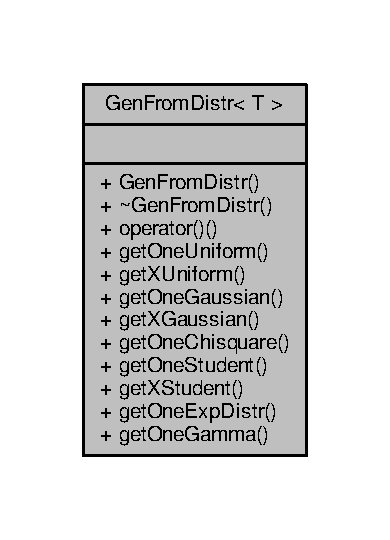
\includegraphics[width=187pt]{classGenFromDistr__coll__graph}
\end{center}
\end{figure}
\subsection*{Public Member Functions}
\begin{DoxyCompactItemize}
\item 
\hyperlink{classGenFromDistr_a9e3401231ba07f8e84c760b892a9eb0a}{Gen\+From\+Distr} (T \&\+\_\+rng)
\item 
\hyperlink{classGenFromDistr_a088eb8a16a206ccffbee7406fc840a90}{$\sim$\+Gen\+From\+Distr} ()
\item 
double \hyperlink{classGenFromDistr_a759d5f09184069456bb02cf0687c04b8}{operator()} ()
\item 
double \hyperlink{classGenFromDistr_a3e32f495d1e6dfa4b152980e8b6c233c}{get\+One\+Uniform} (double a=0., double b=1.)
\item 
Eigen\+::\+Vector\+Xd \hyperlink{classGenFromDistr_af37d022161571f1ed61462b999081b8e}{get\+X\+Uniform} (unsigned int x)
\begin{DoxyCompactList}\small\item\em Generate vector dim x of Uniform random number. \end{DoxyCompactList}\item 
double \hyperlink{classGenFromDistr_aba586e9d1c4d07a30d622e7f16fc13e4}{get\+One\+Gaussian} ()
\item 
Eigen\+::\+Vector\+Xd \hyperlink{classGenFromDistr_a60a61050c09c5f40ad74869a7aa1a6c2}{get\+X\+Gaussian} (unsigned int x)
\begin{DoxyCompactList}\small\item\em Generate vector dim x of Gaussian random number. \end{DoxyCompactList}\item 
double \hyperlink{classGenFromDistr_ad9d10783cc324b3376a078808ba1331b}{get\+One\+Chisquare} (double n)
\item 
double \hyperlink{classGenFromDistr_a7de451b0e96024d6c5216c57a226de76}{get\+One\+Student} (double n)
\item 
Eigen\+::\+Vector\+Xd \hyperlink{classGenFromDistr_a018afaad1a8ea5f4722a412629da610d}{get\+X\+Student} (unsigned int x, double n)
\begin{DoxyCompactList}\small\item\em Generate vector dim x of Student random number. \end{DoxyCompactList}\item 
double \hyperlink{classGenFromDistr_ada0a44362ef21afe2926620f3af489fd}{get\+One\+Exp\+Distr} (double l)
\item 
double \hyperlink{classGenFromDistr_a163dfedc722d8f808ccaae299523db5a}{get\+One\+Gamma} (double a, double b)
\end{DoxyCompactItemize}


\subsection{Detailed Description}
\subsubsection*{template$<$class T$>$\newline
class Gen\+From\+Distr$<$ T $>$}

Generate random number according to specified distribution. 

\subsection{Constructor \& Destructor Documentation}
\hypertarget{classGenFromDistr_a9e3401231ba07f8e84c760b892a9eb0a}{}\label{classGenFromDistr_a9e3401231ba07f8e84c760b892a9eb0a} 
\index{Gen\+From\+Distr@{Gen\+From\+Distr}!Gen\+From\+Distr@{Gen\+From\+Distr}}
\index{Gen\+From\+Distr@{Gen\+From\+Distr}!Gen\+From\+Distr@{Gen\+From\+Distr}}
\subsubsection{\texorpdfstring{Gen\+From\+Distr()}{GenFromDistr()}}
{\footnotesize\ttfamily template$<$class T $>$ \\
\hyperlink{classGenFromDistr}{Gen\+From\+Distr}$<$ T $>$\+::\hyperlink{classGenFromDistr}{Gen\+From\+Distr} (\begin{DoxyParamCaption}\item[{T \&}]{\+\_\+rng }\end{DoxyParamCaption})\hspace{0.3cm}{\ttfamily [inline]}}

\hypertarget{classGenFromDistr_a088eb8a16a206ccffbee7406fc840a90}{}\label{classGenFromDistr_a088eb8a16a206ccffbee7406fc840a90} 
\index{Gen\+From\+Distr@{Gen\+From\+Distr}!````~Gen\+From\+Distr@{$\sim$\+Gen\+From\+Distr}}
\index{````~Gen\+From\+Distr@{$\sim$\+Gen\+From\+Distr}!Gen\+From\+Distr@{Gen\+From\+Distr}}
\subsubsection{\texorpdfstring{$\sim$\+Gen\+From\+Distr()}{~GenFromDistr()}}
{\footnotesize\ttfamily template$<$class T $>$ \\
\hyperlink{classGenFromDistr}{Gen\+From\+Distr}$<$ T $>$\+::$\sim$\hyperlink{classGenFromDistr}{Gen\+From\+Distr} (\begin{DoxyParamCaption}{ }\end{DoxyParamCaption})\hspace{0.3cm}{\ttfamily [inline]}}



\subsection{Member Function Documentation}
\hypertarget{classGenFromDistr_ad9d10783cc324b3376a078808ba1331b}{}\label{classGenFromDistr_ad9d10783cc324b3376a078808ba1331b} 
\index{Gen\+From\+Distr@{Gen\+From\+Distr}!get\+One\+Chisquare@{get\+One\+Chisquare}}
\index{get\+One\+Chisquare@{get\+One\+Chisquare}!Gen\+From\+Distr@{Gen\+From\+Distr}}
\subsubsection{\texorpdfstring{get\+One\+Chisquare()}{getOneChisquare()}}
{\footnotesize\ttfamily template$<$class T $>$ \\
double \hyperlink{classGenFromDistr}{Gen\+From\+Distr}$<$ T $>$\+::get\+One\+Chisquare (\begin{DoxyParamCaption}\item[{double}]{n }\end{DoxyParamCaption})\hspace{0.3cm}{\ttfamily [inline]}}


\begin{DoxyParams}{Parameters}
{\em n} & degree of freedom \\
\hline
\end{DoxyParams}
\hypertarget{classGenFromDistr_ada0a44362ef21afe2926620f3af489fd}{}\label{classGenFromDistr_ada0a44362ef21afe2926620f3af489fd} 
\index{Gen\+From\+Distr@{Gen\+From\+Distr}!get\+One\+Exp\+Distr@{get\+One\+Exp\+Distr}}
\index{get\+One\+Exp\+Distr@{get\+One\+Exp\+Distr}!Gen\+From\+Distr@{Gen\+From\+Distr}}
\subsubsection{\texorpdfstring{get\+One\+Exp\+Distr()}{getOneExpDistr()}}
{\footnotesize\ttfamily template$<$class T $>$ \\
double \hyperlink{classGenFromDistr}{Gen\+From\+Distr}$<$ T $>$\+::get\+One\+Exp\+Distr (\begin{DoxyParamCaption}\item[{double}]{l }\end{DoxyParamCaption})\hspace{0.3cm}{\ttfamily [inline]}}


\begin{DoxyParams}{Parameters}
{\em l} & lambda \\
\hline
\end{DoxyParams}
\hypertarget{classGenFromDistr_a163dfedc722d8f808ccaae299523db5a}{}\label{classGenFromDistr_a163dfedc722d8f808ccaae299523db5a} 
\index{Gen\+From\+Distr@{Gen\+From\+Distr}!get\+One\+Gamma@{get\+One\+Gamma}}
\index{get\+One\+Gamma@{get\+One\+Gamma}!Gen\+From\+Distr@{Gen\+From\+Distr}}
\subsubsection{\texorpdfstring{get\+One\+Gamma()}{getOneGamma()}}
{\footnotesize\ttfamily template$<$class T $>$ \\
double \hyperlink{classGenFromDistr}{Gen\+From\+Distr}$<$ T $>$\+::get\+One\+Gamma (\begin{DoxyParamCaption}\item[{double}]{a,  }\item[{double}]{b }\end{DoxyParamCaption})\hspace{0.3cm}{\ttfamily [inline]}}


\begin{DoxyParams}{Parameters}
{\em a} & $alpha$ \\
\hline
{\em b} & $beta$ \\
\hline
\end{DoxyParams}
\hypertarget{classGenFromDistr_aba586e9d1c4d07a30d622e7f16fc13e4}{}\label{classGenFromDistr_aba586e9d1c4d07a30d622e7f16fc13e4} 
\index{Gen\+From\+Distr@{Gen\+From\+Distr}!get\+One\+Gaussian@{get\+One\+Gaussian}}
\index{get\+One\+Gaussian@{get\+One\+Gaussian}!Gen\+From\+Distr@{Gen\+From\+Distr}}
\subsubsection{\texorpdfstring{get\+One\+Gaussian()}{getOneGaussian()}}
{\footnotesize\ttfamily template$<$class T $>$ \\
double \hyperlink{classGenFromDistr}{Gen\+From\+Distr}$<$ T $>$\+::get\+One\+Gaussian (\begin{DoxyParamCaption}{ }\end{DoxyParamCaption})\hspace{0.3cm}{\ttfamily [inline]}}

\hypertarget{classGenFromDistr_a7de451b0e96024d6c5216c57a226de76}{}\label{classGenFromDistr_a7de451b0e96024d6c5216c57a226de76} 
\index{Gen\+From\+Distr@{Gen\+From\+Distr}!get\+One\+Student@{get\+One\+Student}}
\index{get\+One\+Student@{get\+One\+Student}!Gen\+From\+Distr@{Gen\+From\+Distr}}
\subsubsection{\texorpdfstring{get\+One\+Student()}{getOneStudent()}}
{\footnotesize\ttfamily template$<$class T $>$ \\
double \hyperlink{classGenFromDistr}{Gen\+From\+Distr}$<$ T $>$\+::get\+One\+Student (\begin{DoxyParamCaption}\item[{double}]{n }\end{DoxyParamCaption})\hspace{0.3cm}{\ttfamily [inline]}}


\begin{DoxyParams}{Parameters}
{\em n} & degree of freedom \\
\hline
\end{DoxyParams}
\hypertarget{classGenFromDistr_a3e32f495d1e6dfa4b152980e8b6c233c}{}\label{classGenFromDistr_a3e32f495d1e6dfa4b152980e8b6c233c} 
\index{Gen\+From\+Distr@{Gen\+From\+Distr}!get\+One\+Uniform@{get\+One\+Uniform}}
\index{get\+One\+Uniform@{get\+One\+Uniform}!Gen\+From\+Distr@{Gen\+From\+Distr}}
\subsubsection{\texorpdfstring{get\+One\+Uniform()}{getOneUniform()}}
{\footnotesize\ttfamily template$<$class T $>$ \\
double \hyperlink{classGenFromDistr}{Gen\+From\+Distr}$<$ T $>$\+::get\+One\+Uniform (\begin{DoxyParamCaption}\item[{double}]{a = {\ttfamily 0.},  }\item[{double}]{b = {\ttfamily 1.} }\end{DoxyParamCaption})\hspace{0.3cm}{\ttfamily [inline]}}

\hypertarget{classGenFromDistr_a60a61050c09c5f40ad74869a7aa1a6c2}{}\label{classGenFromDistr_a60a61050c09c5f40ad74869a7aa1a6c2} 
\index{Gen\+From\+Distr@{Gen\+From\+Distr}!get\+X\+Gaussian@{get\+X\+Gaussian}}
\index{get\+X\+Gaussian@{get\+X\+Gaussian}!Gen\+From\+Distr@{Gen\+From\+Distr}}
\subsubsection{\texorpdfstring{get\+X\+Gaussian()}{getXGaussian()}}
{\footnotesize\ttfamily template$<$class T $>$ \\
Eigen\+::\+Vector\+Xd \hyperlink{classGenFromDistr}{Gen\+From\+Distr}$<$ T $>$\+::get\+X\+Gaussian (\begin{DoxyParamCaption}\item[{unsigned int}]{x }\end{DoxyParamCaption})\hspace{0.3cm}{\ttfamily [inline]}}



Generate vector dim x of Gaussian random number. 

\hypertarget{classGenFromDistr_a018afaad1a8ea5f4722a412629da610d}{}\label{classGenFromDistr_a018afaad1a8ea5f4722a412629da610d} 
\index{Gen\+From\+Distr@{Gen\+From\+Distr}!get\+X\+Student@{get\+X\+Student}}
\index{get\+X\+Student@{get\+X\+Student}!Gen\+From\+Distr@{Gen\+From\+Distr}}
\subsubsection{\texorpdfstring{get\+X\+Student()}{getXStudent()}}
{\footnotesize\ttfamily template$<$class T $>$ \\
Eigen\+::\+Vector\+Xd \hyperlink{classGenFromDistr}{Gen\+From\+Distr}$<$ T $>$\+::get\+X\+Student (\begin{DoxyParamCaption}\item[{unsigned int}]{x,  }\item[{double}]{n }\end{DoxyParamCaption})\hspace{0.3cm}{\ttfamily [inline]}}



Generate vector dim x of Student random number. 

\hypertarget{classGenFromDistr_af37d022161571f1ed61462b999081b8e}{}\label{classGenFromDistr_af37d022161571f1ed61462b999081b8e} 
\index{Gen\+From\+Distr@{Gen\+From\+Distr}!get\+X\+Uniform@{get\+X\+Uniform}}
\index{get\+X\+Uniform@{get\+X\+Uniform}!Gen\+From\+Distr@{Gen\+From\+Distr}}
\subsubsection{\texorpdfstring{get\+X\+Uniform()}{getXUniform()}}
{\footnotesize\ttfamily template$<$class T $>$ \\
Eigen\+::\+Vector\+Xd \hyperlink{classGenFromDistr}{Gen\+From\+Distr}$<$ T $>$\+::get\+X\+Uniform (\begin{DoxyParamCaption}\item[{unsigned int}]{x }\end{DoxyParamCaption})\hspace{0.3cm}{\ttfamily [inline]}}



Generate vector dim x of Uniform random number. 

\hypertarget{classGenFromDistr_a759d5f09184069456bb02cf0687c04b8}{}\label{classGenFromDistr_a759d5f09184069456bb02cf0687c04b8} 
\index{Gen\+From\+Distr@{Gen\+From\+Distr}!operator()@{operator()}}
\index{operator()@{operator()}!Gen\+From\+Distr@{Gen\+From\+Distr}}
\subsubsection{\texorpdfstring{operator()()}{operator()()}}
{\footnotesize\ttfamily template$<$class T $>$ \\
double \hyperlink{classGenFromDistr}{Gen\+From\+Distr}$<$ T $>$\+::operator() (\begin{DoxyParamCaption}{ }\end{DoxyParamCaption})\hspace{0.3cm}{\ttfamily [inline]}}



The documentation for this class was generated from the following file\+:\begin{DoxyCompactItemize}
\item 
\hyperlink{generate__rm__from__distr_8h}{generate\+\_\+rm\+\_\+from\+\_\+distr.\+h}\end{DoxyCompactItemize}

\hypertarget{classHistoricalVaR}{}\section{Historical\+VaR Class Reference}
\label{classHistoricalVaR}\index{Historical\+VaR@{Historical\+VaR}}


Compute \hyperlink{classVaR}{VaR} using historical method (histogram method)  




{\ttfamily \#include $<$var\+\_\+model.\+h$>$}



Inheritance diagram for Historical\+VaR\+:
\nopagebreak
\begin{figure}[H]
\begin{center}
\leavevmode
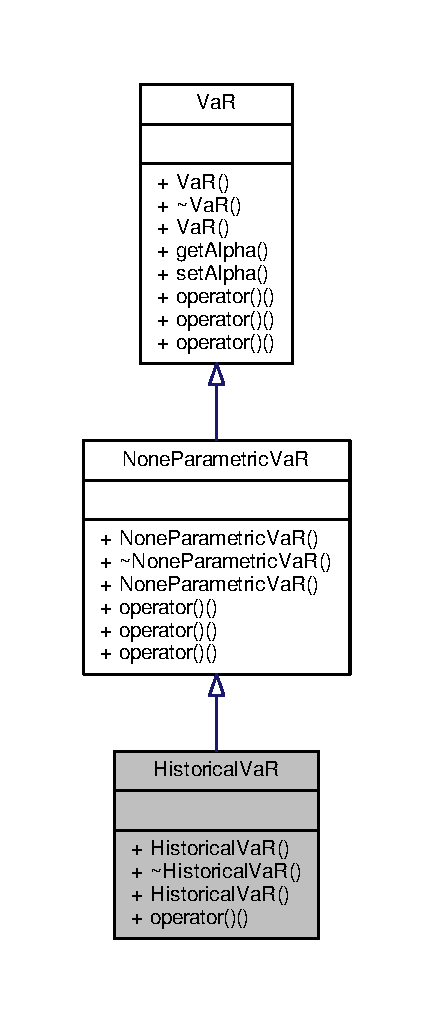
\includegraphics[width=208pt]{classHistoricalVaR__inherit__graph}
\end{center}
\end{figure}


Collaboration diagram for Historical\+VaR\+:
\nopagebreak
\begin{figure}[H]
\begin{center}
\leavevmode
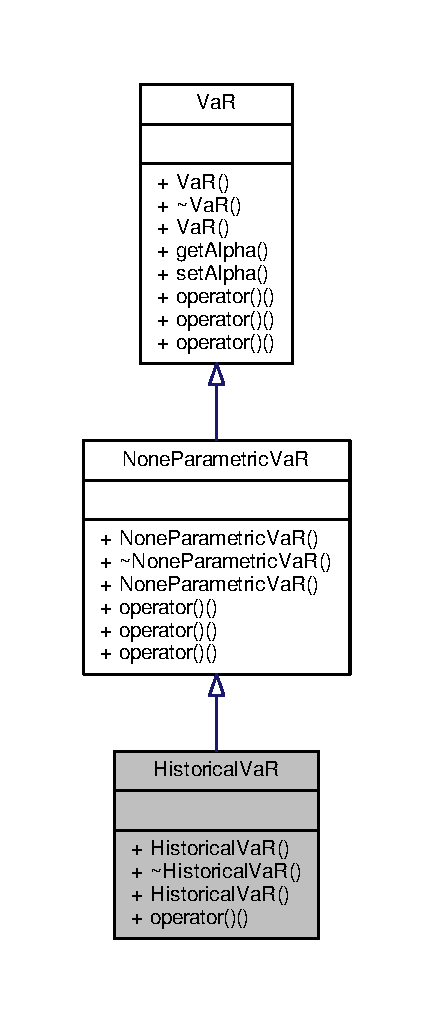
\includegraphics[width=208pt]{classHistoricalVaR__coll__graph}
\end{center}
\end{figure}
\subsection*{Public Member Functions}
\begin{DoxyCompactItemize}
\item 
\hyperlink{classHistoricalVaR_a2f98a84f410ee519c1d08cb3a4e5110f}{Historical\+VaR} (double \+\_\+alpha=.\+05, double \+\_\+lambda=.\+98, \hyperlink{var__model_8h_a05de9d7b6ad30cf17cd8f840666921de}{Weighting\+Scheme} \+\_\+ws=\hyperlink{var__model_8h_a05de9d7b6ad30cf17cd8f840666921deab7e4e0120a041dbe6528b050c04269e0}{none})
\item 
virtual \hyperlink{classHistoricalVaR_ac0b1889d5ba5e3a3efb0d23eaff525a5}{$\sim$\+Historical\+VaR} ()
\item 
\hyperlink{classHistoricalVaR_a75f77512a689c5f4826421e354f3053d}{Historical\+VaR} (const \hyperlink{classHistoricalVaR}{Historical\+VaR} \&other)
\item 
double \hyperlink{classHistoricalVaR_a472b04dc9a4c5989be0e7198bc9c4189}{operator()} (double \+\_\+sigmatminus1, const \hyperlink{compute__returns__eigen_8h_a1eb6a9306ef406d7975f3cbf2e247777}{Vec} \&returns) const
\end{DoxyCompactItemize}


\subsection{Detailed Description}
Compute \hyperlink{classVaR}{VaR} using historical method (histogram method) 

\subsection{Constructor \& Destructor Documentation}
\hypertarget{classHistoricalVaR_a2f98a84f410ee519c1d08cb3a4e5110f}{}\label{classHistoricalVaR_a2f98a84f410ee519c1d08cb3a4e5110f} 
\index{Historical\+VaR@{Historical\+VaR}!Historical\+VaR@{Historical\+VaR}}
\index{Historical\+VaR@{Historical\+VaR}!Historical\+VaR@{Historical\+VaR}}
\subsubsection{\texorpdfstring{Historical\+Va\+R()}{HistoricalVaR()}\hspace{0.1cm}{\footnotesize\ttfamily [1/2]}}
{\footnotesize\ttfamily Historical\+Va\+R\+::\+Historical\+VaR (\begin{DoxyParamCaption}\item[{double}]{\+\_\+alpha = {\ttfamily .05},  }\item[{double}]{\+\_\+lambda = {\ttfamily .98},  }\item[{\hyperlink{var__model_8h_a05de9d7b6ad30cf17cd8f840666921de}{Weighting\+Scheme}}]{\+\_\+ws = {\ttfamily \hyperlink{var__model_8h_a05de9d7b6ad30cf17cd8f840666921deab7e4e0120a041dbe6528b050c04269e0}{none}} }\end{DoxyParamCaption})}

\hypertarget{classHistoricalVaR_ac0b1889d5ba5e3a3efb0d23eaff525a5}{}\label{classHistoricalVaR_ac0b1889d5ba5e3a3efb0d23eaff525a5} 
\index{Historical\+VaR@{Historical\+VaR}!````~Historical\+VaR@{$\sim$\+Historical\+VaR}}
\index{````~Historical\+VaR@{$\sim$\+Historical\+VaR}!Historical\+VaR@{Historical\+VaR}}
\subsubsection{\texorpdfstring{$\sim$\+Historical\+Va\+R()}{~HistoricalVaR()}}
{\footnotesize\ttfamily virtual Historical\+Va\+R\+::$\sim$\+Historical\+VaR (\begin{DoxyParamCaption}{ }\end{DoxyParamCaption})\hspace{0.3cm}{\ttfamily [inline]}, {\ttfamily [virtual]}}

\hypertarget{classHistoricalVaR_a75f77512a689c5f4826421e354f3053d}{}\label{classHistoricalVaR_a75f77512a689c5f4826421e354f3053d} 
\index{Historical\+VaR@{Historical\+VaR}!Historical\+VaR@{Historical\+VaR}}
\index{Historical\+VaR@{Historical\+VaR}!Historical\+VaR@{Historical\+VaR}}
\subsubsection{\texorpdfstring{Historical\+Va\+R()}{HistoricalVaR()}\hspace{0.1cm}{\footnotesize\ttfamily [2/2]}}
{\footnotesize\ttfamily Historical\+Va\+R\+::\+Historical\+VaR (\begin{DoxyParamCaption}\item[{const \hyperlink{classHistoricalVaR}{Historical\+VaR} \&}]{other }\end{DoxyParamCaption})}



\subsection{Member Function Documentation}
\hypertarget{classHistoricalVaR_a472b04dc9a4c5989be0e7198bc9c4189}{}\label{classHistoricalVaR_a472b04dc9a4c5989be0e7198bc9c4189} 
\index{Historical\+VaR@{Historical\+VaR}!operator()@{operator()}}
\index{operator()@{operator()}!Historical\+VaR@{Historical\+VaR}}
\subsubsection{\texorpdfstring{operator()()}{operator()()}}
{\footnotesize\ttfamily double Historical\+Va\+R\+::operator() (\begin{DoxyParamCaption}\item[{double}]{\+\_\+sigmatminus1,  }\item[{const \hyperlink{compute__returns__eigen_8h_a1eb6a9306ef406d7975f3cbf2e247777}{Vec} \&}]{returns }\end{DoxyParamCaption}) const\hspace{0.3cm}{\ttfamily [virtual]}}



Implements \hyperlink{classNoneParametricVaR_a958aae1b9bc03a8ef87295df30db76f7}{None\+Parametric\+VaR}.



The documentation for this class was generated from the following file\+:\begin{DoxyCompactItemize}
\item 
\hyperlink{var__model_8h}{var\+\_\+model.\+h}\end{DoxyCompactItemize}

\hypertarget{classInstrument}{}\section{Instrument Class Reference}
\label{classInstrument}\index{Instrument@{Instrument}}


{\ttfamily \#include $<$instrument.\+h$>$}



Inheritance diagram for Instrument\+:
\nopagebreak
\begin{figure}[H]
\begin{center}
\leavevmode
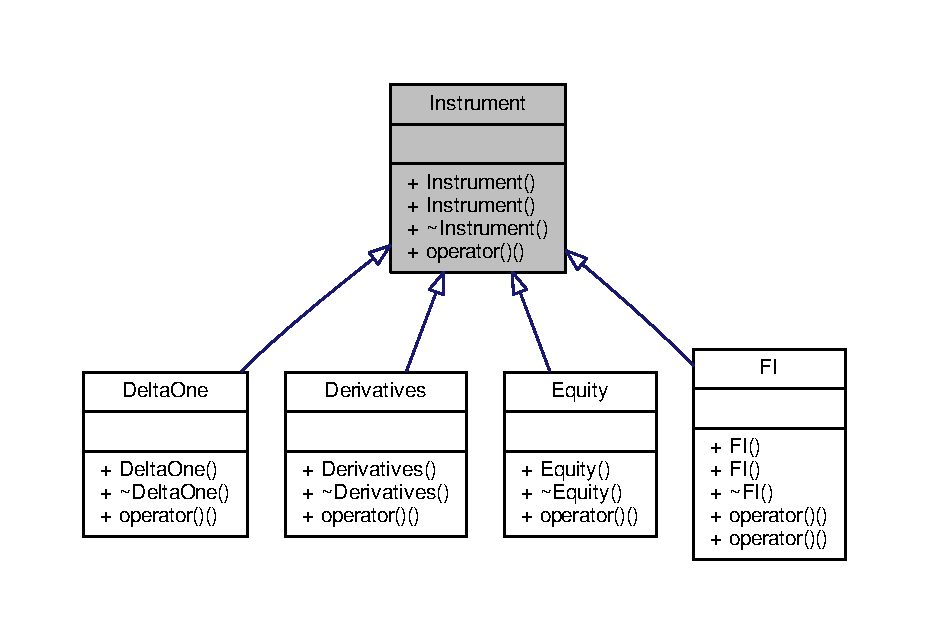
\includegraphics[width=350pt]{classInstrument__inherit__graph}
\end{center}
\end{figure}


Collaboration diagram for Instrument\+:
\nopagebreak
\begin{figure}[H]
\begin{center}
\leavevmode
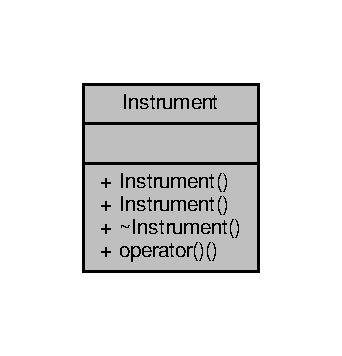
\includegraphics[width=164pt]{classInstrument__coll__graph}
\end{center}
\end{figure}
\subsection*{Public Member Functions}
\begin{DoxyCompactItemize}
\item 
\hyperlink{classInstrument_a1a297b2cbe1e239c8ede2e90185e2880}{Instrument} ()
\item 
\hyperlink{classInstrument_a2704ef015e35f22e444f8e15ece24be0}{Instrument} (const \hyperlink{classInstrument}{Instrument} \&other)
\item 
virtual \hyperlink{classInstrument_a28512cef5ccbedc9094876866f06f921}{$\sim$\+Instrument} ()
\item 
virtual double \hyperlink{classInstrument_a33b6faccaeb494858dee5c547de897b6}{operator()} (double rtn) const =0
\begin{DoxyCompactList}\small\item\em Compute an approximation on P\&L of instrument following shock. \end{DoxyCompactList}\end{DoxyCompactItemize}


\subsection{Detailed Description}
Does not attempt to make full re-\/evaluation on the ptf.

Use approximation approach instead 

\subsection{Constructor \& Destructor Documentation}
\hypertarget{classInstrument_a1a297b2cbe1e239c8ede2e90185e2880}{}\label{classInstrument_a1a297b2cbe1e239c8ede2e90185e2880} 
\index{Instrument@{Instrument}!Instrument@{Instrument}}
\index{Instrument@{Instrument}!Instrument@{Instrument}}
\subsubsection{\texorpdfstring{Instrument()}{Instrument()}\hspace{0.1cm}{\footnotesize\ttfamily [1/2]}}
{\footnotesize\ttfamily Instrument\+::\+Instrument (\begin{DoxyParamCaption}{ }\end{DoxyParamCaption})\hspace{0.3cm}{\ttfamily [inline]}}

\hypertarget{classInstrument_a2704ef015e35f22e444f8e15ece24be0}{}\label{classInstrument_a2704ef015e35f22e444f8e15ece24be0} 
\index{Instrument@{Instrument}!Instrument@{Instrument}}
\index{Instrument@{Instrument}!Instrument@{Instrument}}
\subsubsection{\texorpdfstring{Instrument()}{Instrument()}\hspace{0.1cm}{\footnotesize\ttfamily [2/2]}}
{\footnotesize\ttfamily Instrument\+::\+Instrument (\begin{DoxyParamCaption}\item[{const \hyperlink{classInstrument}{Instrument} \&}]{other }\end{DoxyParamCaption})}

\hypertarget{classInstrument_a28512cef5ccbedc9094876866f06f921}{}\label{classInstrument_a28512cef5ccbedc9094876866f06f921} 
\index{Instrument@{Instrument}!````~Instrument@{$\sim$\+Instrument}}
\index{````~Instrument@{$\sim$\+Instrument}!Instrument@{Instrument}}
\subsubsection{\texorpdfstring{$\sim$\+Instrument()}{~Instrument()}}
{\footnotesize\ttfamily virtual Instrument\+::$\sim$\+Instrument (\begin{DoxyParamCaption}{ }\end{DoxyParamCaption})\hspace{0.3cm}{\ttfamily [inline]}, {\ttfamily [virtual]}}



\subsection{Member Function Documentation}
\hypertarget{classInstrument_a33b6faccaeb494858dee5c547de897b6}{}\label{classInstrument_a33b6faccaeb494858dee5c547de897b6} 
\index{Instrument@{Instrument}!operator()@{operator()}}
\index{operator()@{operator()}!Instrument@{Instrument}}
\subsubsection{\texorpdfstring{operator()()}{operator()()}}
{\footnotesize\ttfamily virtual double Instrument\+::operator() (\begin{DoxyParamCaption}\item[{double}]{rtn }\end{DoxyParamCaption}) const\hspace{0.3cm}{\ttfamily [pure virtual]}}



Compute an approximation on P\&L of instrument following shock. 



Implemented in \hyperlink{classFI_a99ad4380e8178d7fd304597622a2c05c}{FI}, \hyperlink{classDerivatives_a765ecae139ee81fb5143a20462211623}{Derivatives}, \hyperlink{classEquity_a2844b7fa3dd164ce216909d1fe958c9f}{Equity}, and \hyperlink{classDeltaOne_a8dd4b5243412ab399b07c1128262f570}{Delta\+One}.



The documentation for this class was generated from the following file\+:\begin{DoxyCompactItemize}
\item 
\hyperlink{instrument_8h}{instrument.\+h}\end{DoxyCompactItemize}

\hypertarget{classMCEngine}{}\section{M\+C\+Engine$<$ T, U $>$ Class Template Reference}
\label{classMCEngine}\index{M\+C\+Engine$<$ T, U $>$@{M\+C\+Engine$<$ T, U $>$}}


Student\textquotesingle{}s t-\/distr.  




{\ttfamily \#include $<$mc\+\_\+engine.\+h$>$}



Inheritance diagram for M\+C\+Engine$<$ T, U $>$\+:
\nopagebreak
\begin{figure}[H]
\begin{center}
\leavevmode
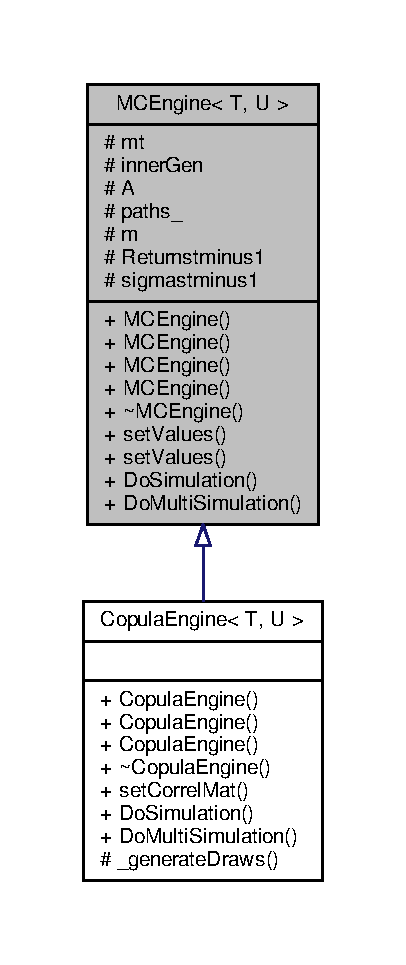
\includegraphics[width=195pt]{classMCEngine__inherit__graph}
\end{center}
\end{figure}


Collaboration diagram for M\+C\+Engine$<$ T, U $>$\+:
\nopagebreak
\begin{figure}[H]
\begin{center}
\leavevmode
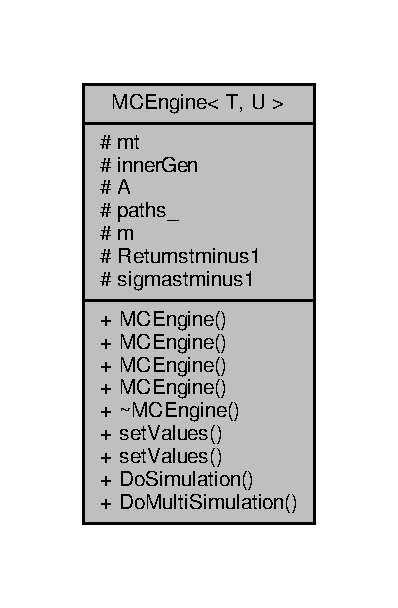
\includegraphics[width=191pt]{classMCEngine__coll__graph}
\end{center}
\end{figure}
\subsection*{Public Types}
\begin{DoxyCompactItemize}
\item 
typedef std\+::vector$<$ U $>$ \hyperlink{classMCEngine_a977f1048508a1467c496c2c47231d1d3}{paths}
\end{DoxyCompactItemize}
\subsection*{Public Member Functions}
\begin{DoxyCompactItemize}
\item 
\hyperlink{classMCEngine_a2021419bc32829220a41a42e0b7ddca3}{M\+C\+Engine} (T \&\+\_\+rng, const U \&\+\_\+path)
\begin{DoxyCompactList}\small\item\em Constructor 2x overloads. \end{DoxyCompactList}\item 
\hyperlink{classMCEngine_a1d6bcdacaa99b8f75a89c9b2c344bd0d}{M\+C\+Engine} (T \&\+\_\+rng, const \hyperlink{classMCEngine_a977f1048508a1467c496c2c47231d1d3}{paths} \&\+\_\+paths, const Eigen\+::\+Matrix\+Xd \&\+\_\+A, \hyperlink{mc__engine_8h_aac1fa89c4c60883790b2adb885048486}{mat\+Type} \+\_\+mt)
\begin{DoxyCompactList}\small\item\em multiple assets \end{DoxyCompactList}\item 
\hyperlink{classMCEngine_a51e0bc14bc95f352654e7caaad78ecfb}{M\+C\+Engine} (T \&\+\_\+rng, const \hyperlink{classMCEngine_a977f1048508a1467c496c2c47231d1d3}{paths} \&\+\_\+paths)
\begin{DoxyCompactList}\small\item\em multiple assets w/o correl matrix \end{DoxyCompactList}\item 
\hyperlink{classMCEngine_a2341fbbbe2e92f91e4672757a1f8fea3}{M\+C\+Engine} (const \hyperlink{classMCEngine}{M\+C\+Engine} \&other)
\item 
virtual \hyperlink{classMCEngine_a9e6d34c928e8a7c7fd3cf25efc18a56a}{$\sim$\+M\+C\+Engine} ()
\item 
void \hyperlink{classMCEngine_a28f2f449e07eb22e0ae9caadfc919a3e}{set\+Values} (const \hyperlink{compute__returns__eigen_8h_a1eb6a9306ef406d7975f3cbf2e247777}{Vec} \&rtns, const double vol)
\item 
void \hyperlink{classMCEngine_ab95a4a68842966a18f2bc8ef74dabf1f}{set\+Values} (const \hyperlink{compute__returns__eigen_8h_ae14dd28696f743e067dbd2594616bad6}{Mat} \&rtns, const \hyperlink{compute__returns__eigen_8h_a1eb6a9306ef406d7975f3cbf2e247777}{Vec} \&vol)
\item 
\hyperlink{compute__returns__eigen_8h_a1eb6a9306ef406d7975f3cbf2e247777}{Vec} \hyperlink{classMCEngine_a2e84a3728e2fcea5999c472077ddeb14}{Do\+Simulation} (size\+\_\+t p=0, double n=1.e+05, \hyperlink{mc__engine_8h_aeb3b337d49b67199ac031f705d206198}{underlying\+Process} up=\hyperlink{mc__engine_8h_aeb3b337d49b67199ac031f705d206198aa11844f44df96808eb4e519ba04f088c}{Gaussian})
\item 
\hyperlink{compute__returns__eigen_8h_ae14dd28696f743e067dbd2594616bad6}{Mat} \hyperlink{classMCEngine_a15873abff351cca971b1154f7ffe40b5}{Do\+Multi\+Simulation} (double n=1.e+05, \hyperlink{mc__engine_8h_aeb3b337d49b67199ac031f705d206198}{underlying\+Process} up=\hyperlink{mc__engine_8h_aeb3b337d49b67199ac031f705d206198aa11844f44df96808eb4e519ba04f088c}{Gaussian})
\end{DoxyCompactItemize}
\subsection*{Protected Attributes}
\begin{DoxyCompactItemize}
\item 
\hyperlink{mc__engine_8h_aac1fa89c4c60883790b2adb885048486}{mat\+Type} \hyperlink{classMCEngine_a66aed856c87b6ad40107b50e229da831}{mt}
\item 
T \hyperlink{classMCEngine_ae365d3f22ff95cdd7efbd9b555e81a3b}{inner\+Gen}
\item 
Eigen\+::\+Matrix\+Xd \hyperlink{classMCEngine_a916324fa45d5e3288e5792fc769c1ded}{A}
\item 
\hyperlink{classMCEngine_a977f1048508a1467c496c2c47231d1d3}{paths} \hyperlink{classMCEngine_a138035de4a3c8e088c437da6d6079ded}{paths\+\_\+}
\item 
size\+\_\+t \hyperlink{classMCEngine_a56d5cb47b251de9dd585af4ce6f32c18}{m}
\item 
\hyperlink{compute__returns__eigen_8h_ae14dd28696f743e067dbd2594616bad6}{Mat} \hyperlink{classMCEngine_a74547ec91afe270f4b0efc13048852dc}{Returnstminus1}
\item 
\hyperlink{compute__returns__eigen_8h_a1eb6a9306ef406d7975f3cbf2e247777}{Vec} \hyperlink{classMCEngine_afbebad3416f7c4eb6527497d19366f82}{sigmastminus1}
\end{DoxyCompactItemize}


\subsection{Detailed Description}
\subsubsection*{template$<$class T, class U$>$\newline
class M\+C\+Engine$<$ T, U $>$}

Student\textquotesingle{}s t-\/distr. 

Simulate return through Monte-\/\+Carlo T rng, U path 

\subsection{Member Typedef Documentation}
\hypertarget{classMCEngine_a977f1048508a1467c496c2c47231d1d3}{}\label{classMCEngine_a977f1048508a1467c496c2c47231d1d3} 
\index{M\+C\+Engine@{M\+C\+Engine}!paths@{paths}}
\index{paths@{paths}!M\+C\+Engine@{M\+C\+Engine}}
\subsubsection{\texorpdfstring{paths}{paths}}
{\footnotesize\ttfamily template$<$class T, class U$>$ \\
typedef std\+::vector$<$U$>$ \hyperlink{classMCEngine}{M\+C\+Engine}$<$ T, U $>$\+::\hyperlink{classMCEngine_a977f1048508a1467c496c2c47231d1d3}{paths}}



\subsection{Constructor \& Destructor Documentation}
\hypertarget{classMCEngine_a2021419bc32829220a41a42e0b7ddca3}{}\label{classMCEngine_a2021419bc32829220a41a42e0b7ddca3} 
\index{M\+C\+Engine@{M\+C\+Engine}!M\+C\+Engine@{M\+C\+Engine}}
\index{M\+C\+Engine@{M\+C\+Engine}!M\+C\+Engine@{M\+C\+Engine}}
\subsubsection{\texorpdfstring{M\+C\+Engine()}{MCEngine()}\hspace{0.1cm}{\footnotesize\ttfamily [1/4]}}
{\footnotesize\ttfamily template$<$class T, class U$>$ \\
\hyperlink{classMCEngine}{M\+C\+Engine}$<$ T, U $>$\+::\hyperlink{classMCEngine}{M\+C\+Engine} (\begin{DoxyParamCaption}\item[{T \&}]{\+\_\+rng,  }\item[{const U \&}]{\+\_\+path }\end{DoxyParamCaption})\hspace{0.3cm}{\ttfamily [inline]}}



Constructor 2x overloads. 

\hypertarget{classMCEngine_a1d6bcdacaa99b8f75a89c9b2c344bd0d}{}\label{classMCEngine_a1d6bcdacaa99b8f75a89c9b2c344bd0d} 
\index{M\+C\+Engine@{M\+C\+Engine}!M\+C\+Engine@{M\+C\+Engine}}
\index{M\+C\+Engine@{M\+C\+Engine}!M\+C\+Engine@{M\+C\+Engine}}
\subsubsection{\texorpdfstring{M\+C\+Engine()}{MCEngine()}\hspace{0.1cm}{\footnotesize\ttfamily [2/4]}}
{\footnotesize\ttfamily template$<$class T, class U$>$ \\
\hyperlink{classMCEngine}{M\+C\+Engine}$<$ T, U $>$\+::\hyperlink{classMCEngine}{M\+C\+Engine} (\begin{DoxyParamCaption}\item[{T \&}]{\+\_\+rng,  }\item[{const \hyperlink{classMCEngine_a977f1048508a1467c496c2c47231d1d3}{paths} \&}]{\+\_\+paths,  }\item[{const Eigen\+::\+Matrix\+Xd \&}]{\+\_\+A,  }\item[{\hyperlink{mc__engine_8h_aac1fa89c4c60883790b2adb885048486}{mat\+Type}}]{\+\_\+mt }\end{DoxyParamCaption})\hspace{0.3cm}{\ttfamily [inline]}}



multiple assets 

\hypertarget{classMCEngine_a51e0bc14bc95f352654e7caaad78ecfb}{}\label{classMCEngine_a51e0bc14bc95f352654e7caaad78ecfb} 
\index{M\+C\+Engine@{M\+C\+Engine}!M\+C\+Engine@{M\+C\+Engine}}
\index{M\+C\+Engine@{M\+C\+Engine}!M\+C\+Engine@{M\+C\+Engine}}
\subsubsection{\texorpdfstring{M\+C\+Engine()}{MCEngine()}\hspace{0.1cm}{\footnotesize\ttfamily [3/4]}}
{\footnotesize\ttfamily template$<$class T, class U$>$ \\
\hyperlink{classMCEngine}{M\+C\+Engine}$<$ T, U $>$\+::\hyperlink{classMCEngine}{M\+C\+Engine} (\begin{DoxyParamCaption}\item[{T \&}]{\+\_\+rng,  }\item[{const \hyperlink{classMCEngine_a977f1048508a1467c496c2c47231d1d3}{paths} \&}]{\+\_\+paths }\end{DoxyParamCaption})\hspace{0.3cm}{\ttfamily [inline]}}



multiple assets w/o correl matrix 

\hypertarget{classMCEngine_a2341fbbbe2e92f91e4672757a1f8fea3}{}\label{classMCEngine_a2341fbbbe2e92f91e4672757a1f8fea3} 
\index{M\+C\+Engine@{M\+C\+Engine}!M\+C\+Engine@{M\+C\+Engine}}
\index{M\+C\+Engine@{M\+C\+Engine}!M\+C\+Engine@{M\+C\+Engine}}
\subsubsection{\texorpdfstring{M\+C\+Engine()}{MCEngine()}\hspace{0.1cm}{\footnotesize\ttfamily [4/4]}}
{\footnotesize\ttfamily template$<$class T, class U$>$ \\
\hyperlink{classMCEngine}{M\+C\+Engine}$<$ T, U $>$\+::\hyperlink{classMCEngine}{M\+C\+Engine} (\begin{DoxyParamCaption}\item[{const \hyperlink{classMCEngine}{M\+C\+Engine}$<$ T, U $>$ \&}]{other }\end{DoxyParamCaption})\hspace{0.3cm}{\ttfamily [inline]}}

\hypertarget{classMCEngine_a9e6d34c928e8a7c7fd3cf25efc18a56a}{}\label{classMCEngine_a9e6d34c928e8a7c7fd3cf25efc18a56a} 
\index{M\+C\+Engine@{M\+C\+Engine}!````~M\+C\+Engine@{$\sim$\+M\+C\+Engine}}
\index{````~M\+C\+Engine@{$\sim$\+M\+C\+Engine}!M\+C\+Engine@{M\+C\+Engine}}
\subsubsection{\texorpdfstring{$\sim$\+M\+C\+Engine()}{~MCEngine()}}
{\footnotesize\ttfamily template$<$class T, class U$>$ \\
virtual \hyperlink{classMCEngine}{M\+C\+Engine}$<$ T, U $>$\+::$\sim$\hyperlink{classMCEngine}{M\+C\+Engine} (\begin{DoxyParamCaption}{ }\end{DoxyParamCaption})\hspace{0.3cm}{\ttfamily [inline]}, {\ttfamily [virtual]}}



\subsection{Member Function Documentation}
\hypertarget{classMCEngine_a15873abff351cca971b1154f7ffe40b5}{}\label{classMCEngine_a15873abff351cca971b1154f7ffe40b5} 
\index{M\+C\+Engine@{M\+C\+Engine}!Do\+Multi\+Simulation@{Do\+Multi\+Simulation}}
\index{Do\+Multi\+Simulation@{Do\+Multi\+Simulation}!M\+C\+Engine@{M\+C\+Engine}}
\subsubsection{\texorpdfstring{Do\+Multi\+Simulation()}{DoMultiSimulation()}}
{\footnotesize\ttfamily template$<$class T, class U$>$ \\
\hyperlink{compute__returns__eigen_8h_ae14dd28696f743e067dbd2594616bad6}{Mat} \hyperlink{classMCEngine}{M\+C\+Engine}$<$ T, U $>$\+::Do\+Multi\+Simulation (\begin{DoxyParamCaption}\item[{double}]{n = {\ttfamily 1.e+05},  }\item[{\hyperlink{mc__engine_8h_aeb3b337d49b67199ac031f705d206198}{underlying\+Process}}]{up = {\ttfamily \hyperlink{mc__engine_8h_aeb3b337d49b67199ac031f705d206198aa11844f44df96808eb4e519ba04f088c}{Gaussian}} }\end{DoxyParamCaption})\hspace{0.3cm}{\ttfamily [inline]}}

multiple indep rtn with Cholesky decomposition to produce correl rtns

mutliple indep rtn with principal component \hypertarget{classMCEngine_a2e84a3728e2fcea5999c472077ddeb14}{}\label{classMCEngine_a2e84a3728e2fcea5999c472077ddeb14} 
\index{M\+C\+Engine@{M\+C\+Engine}!Do\+Simulation@{Do\+Simulation}}
\index{Do\+Simulation@{Do\+Simulation}!M\+C\+Engine@{M\+C\+Engine}}
\subsubsection{\texorpdfstring{Do\+Simulation()}{DoSimulation()}}
{\footnotesize\ttfamily template$<$class T, class U$>$ \\
\hyperlink{compute__returns__eigen_8h_a1eb6a9306ef406d7975f3cbf2e247777}{Vec} \hyperlink{classMCEngine}{M\+C\+Engine}$<$ T, U $>$\+::Do\+Simulation (\begin{DoxyParamCaption}\item[{size\+\_\+t}]{p = {\ttfamily 0},  }\item[{double}]{n = {\ttfamily 1.e+05},  }\item[{\hyperlink{mc__engine_8h_aeb3b337d49b67199ac031f705d206198}{underlying\+Process}}]{up = {\ttfamily \hyperlink{mc__engine_8h_aeb3b337d49b67199ac031f705d206198aa11844f44df96808eb4e519ba04f088c}{Gaussian}} }\end{DoxyParamCaption})\hspace{0.3cm}{\ttfamily [inline]}}

\hypertarget{classMCEngine_a28f2f449e07eb22e0ae9caadfc919a3e}{}\label{classMCEngine_a28f2f449e07eb22e0ae9caadfc919a3e} 
\index{M\+C\+Engine@{M\+C\+Engine}!set\+Values@{set\+Values}}
\index{set\+Values@{set\+Values}!M\+C\+Engine@{M\+C\+Engine}}
\subsubsection{\texorpdfstring{set\+Values()}{setValues()}\hspace{0.1cm}{\footnotesize\ttfamily [1/2]}}
{\footnotesize\ttfamily template$<$class T, class U$>$ \\
void \hyperlink{classMCEngine}{M\+C\+Engine}$<$ T, U $>$\+::set\+Values (\begin{DoxyParamCaption}\item[{const \hyperlink{compute__returns__eigen_8h_a1eb6a9306ef406d7975f3cbf2e247777}{Vec} \&}]{rtns,  }\item[{const double}]{vol }\end{DoxyParamCaption})\hspace{0.3cm}{\ttfamily [inline]}}

\hypertarget{classMCEngine_ab95a4a68842966a18f2bc8ef74dabf1f}{}\label{classMCEngine_ab95a4a68842966a18f2bc8ef74dabf1f} 
\index{M\+C\+Engine@{M\+C\+Engine}!set\+Values@{set\+Values}}
\index{set\+Values@{set\+Values}!M\+C\+Engine@{M\+C\+Engine}}
\subsubsection{\texorpdfstring{set\+Values()}{setValues()}\hspace{0.1cm}{\footnotesize\ttfamily [2/2]}}
{\footnotesize\ttfamily template$<$class T, class U$>$ \\
void \hyperlink{classMCEngine}{M\+C\+Engine}$<$ T, U $>$\+::set\+Values (\begin{DoxyParamCaption}\item[{const \hyperlink{compute__returns__eigen_8h_ae14dd28696f743e067dbd2594616bad6}{Mat} \&}]{rtns,  }\item[{const \hyperlink{compute__returns__eigen_8h_a1eb6a9306ef406d7975f3cbf2e247777}{Vec} \&}]{vol }\end{DoxyParamCaption})\hspace{0.3cm}{\ttfamily [inline]}}



\subsection{Member Data Documentation}
\hypertarget{classMCEngine_a916324fa45d5e3288e5792fc769c1ded}{}\label{classMCEngine_a916324fa45d5e3288e5792fc769c1ded} 
\index{M\+C\+Engine@{M\+C\+Engine}!A@{A}}
\index{A@{A}!M\+C\+Engine@{M\+C\+Engine}}
\subsubsection{\texorpdfstring{A}{A}}
{\footnotesize\ttfamily template$<$class T, class U$>$ \\
Eigen\+::\+Matrix\+Xd \hyperlink{classMCEngine}{M\+C\+Engine}$<$ T, U $>$\+::A\hspace{0.3cm}{\ttfamily [protected]}}

\hypertarget{classMCEngine_ae365d3f22ff95cdd7efbd9b555e81a3b}{}\label{classMCEngine_ae365d3f22ff95cdd7efbd9b555e81a3b} 
\index{M\+C\+Engine@{M\+C\+Engine}!inner\+Gen@{inner\+Gen}}
\index{inner\+Gen@{inner\+Gen}!M\+C\+Engine@{M\+C\+Engine}}
\subsubsection{\texorpdfstring{inner\+Gen}{innerGen}}
{\footnotesize\ttfamily template$<$class T, class U$>$ \\
T \hyperlink{classMCEngine}{M\+C\+Engine}$<$ T, U $>$\+::inner\+Gen\hspace{0.3cm}{\ttfamily [protected]}}

\hypertarget{classMCEngine_a56d5cb47b251de9dd585af4ce6f32c18}{}\label{classMCEngine_a56d5cb47b251de9dd585af4ce6f32c18} 
\index{M\+C\+Engine@{M\+C\+Engine}!m@{m}}
\index{m@{m}!M\+C\+Engine@{M\+C\+Engine}}
\subsubsection{\texorpdfstring{m}{m}}
{\footnotesize\ttfamily template$<$class T, class U$>$ \\
size\+\_\+t \hyperlink{classMCEngine}{M\+C\+Engine}$<$ T, U $>$\+::m\hspace{0.3cm}{\ttfamily [protected]}}

\hypertarget{classMCEngine_a66aed856c87b6ad40107b50e229da831}{}\label{classMCEngine_a66aed856c87b6ad40107b50e229da831} 
\index{M\+C\+Engine@{M\+C\+Engine}!mt@{mt}}
\index{mt@{mt}!M\+C\+Engine@{M\+C\+Engine}}
\subsubsection{\texorpdfstring{mt}{mt}}
{\footnotesize\ttfamily template$<$class T, class U$>$ \\
\hyperlink{mc__engine_8h_aac1fa89c4c60883790b2adb885048486}{mat\+Type} \hyperlink{classMCEngine}{M\+C\+Engine}$<$ T, U $>$\+::mt\hspace{0.3cm}{\ttfamily [protected]}}

\hypertarget{classMCEngine_a138035de4a3c8e088c437da6d6079ded}{}\label{classMCEngine_a138035de4a3c8e088c437da6d6079ded} 
\index{M\+C\+Engine@{M\+C\+Engine}!paths\+\_\+@{paths\+\_\+}}
\index{paths\+\_\+@{paths\+\_\+}!M\+C\+Engine@{M\+C\+Engine}}
\subsubsection{\texorpdfstring{paths\+\_\+}{paths\_}}
{\footnotesize\ttfamily template$<$class T, class U$>$ \\
\hyperlink{classMCEngine_a977f1048508a1467c496c2c47231d1d3}{paths} \hyperlink{classMCEngine}{M\+C\+Engine}$<$ T, U $>$\+::paths\+\_\+\hspace{0.3cm}{\ttfamily [protected]}}

\hypertarget{classMCEngine_a74547ec91afe270f4b0efc13048852dc}{}\label{classMCEngine_a74547ec91afe270f4b0efc13048852dc} 
\index{M\+C\+Engine@{M\+C\+Engine}!Returnstminus1@{Returnstminus1}}
\index{Returnstminus1@{Returnstminus1}!M\+C\+Engine@{M\+C\+Engine}}
\subsubsection{\texorpdfstring{Returnstminus1}{Returnstminus1}}
{\footnotesize\ttfamily template$<$class T, class U$>$ \\
\hyperlink{compute__returns__eigen_8h_ae14dd28696f743e067dbd2594616bad6}{Mat} \hyperlink{classMCEngine}{M\+C\+Engine}$<$ T, U $>$\+::Returnstminus1\hspace{0.3cm}{\ttfamily [protected]}}

\hypertarget{classMCEngine_afbebad3416f7c4eb6527497d19366f82}{}\label{classMCEngine_afbebad3416f7c4eb6527497d19366f82} 
\index{M\+C\+Engine@{M\+C\+Engine}!sigmastminus1@{sigmastminus1}}
\index{sigmastminus1@{sigmastminus1}!M\+C\+Engine@{M\+C\+Engine}}
\subsubsection{\texorpdfstring{sigmastminus1}{sigmastminus1}}
{\footnotesize\ttfamily template$<$class T, class U$>$ \\
\hyperlink{compute__returns__eigen_8h_a1eb6a9306ef406d7975f3cbf2e247777}{Vec} \hyperlink{classMCEngine}{M\+C\+Engine}$<$ T, U $>$\+::sigmastminus1\hspace{0.3cm}{\ttfamily [protected]}}



The documentation for this class was generated from the following file\+:\begin{DoxyCompactItemize}
\item 
\hyperlink{mc__engine_8h}{mc\+\_\+engine.\+h}\end{DoxyCompactItemize}

\hypertarget{classNoneParametricVaR}{}\section{None\+Parametric\+VaR Class Reference}
\label{classNoneParametricVaR}\index{None\+Parametric\+VaR@{None\+Parametric\+VaR}}


{\ttfamily \#include $<$var\+\_\+model.\+h$>$}



Inheritance diagram for None\+Parametric\+VaR\+:
\nopagebreak
\begin{figure}[H]
\begin{center}
\leavevmode
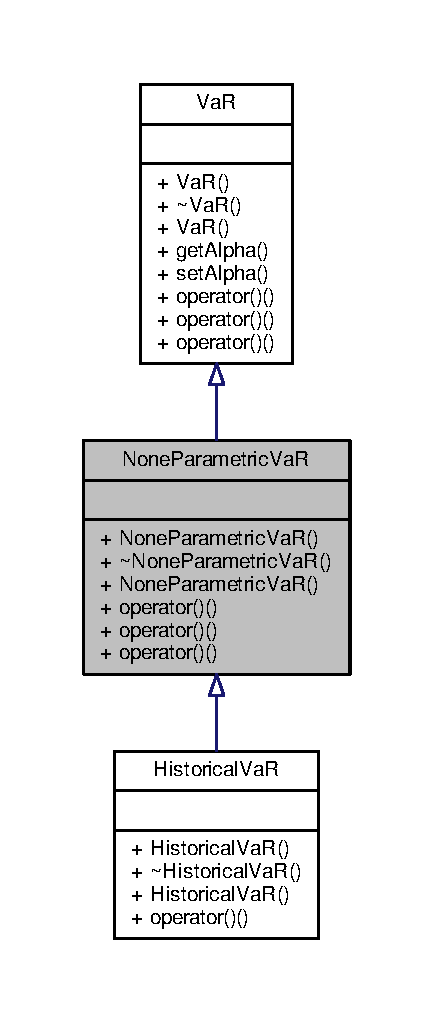
\includegraphics[width=208pt]{classNoneParametricVaR__inherit__graph}
\end{center}
\end{figure}


Collaboration diagram for None\+Parametric\+VaR\+:
\nopagebreak
\begin{figure}[H]
\begin{center}
\leavevmode
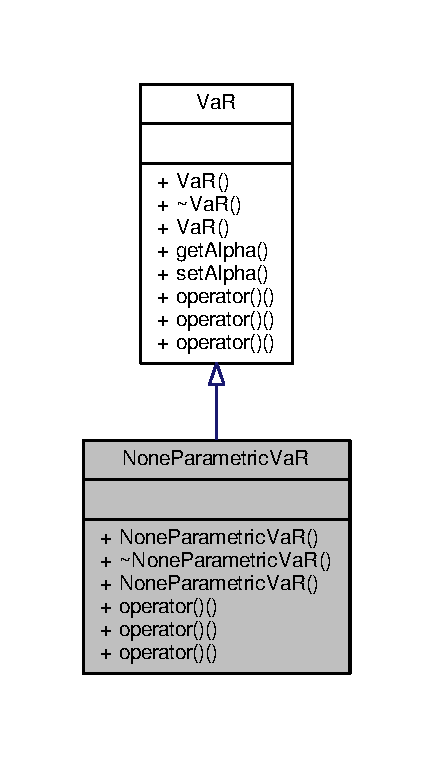
\includegraphics[width=208pt]{classNoneParametricVaR__coll__graph}
\end{center}
\end{figure}
\subsection*{Public Member Functions}
\begin{DoxyCompactItemize}
\item 
\hyperlink{classNoneParametricVaR_a0d9d38576c718b01b2ce865e2edaf84e}{None\+Parametric\+VaR} (double \+\_\+alpha=.\+05)
\item 
virtual \hyperlink{classNoneParametricVaR_aac413dea6f621cbe6e1f5037665296c0}{$\sim$\+None\+Parametric\+VaR} ()
\item 
\hyperlink{classNoneParametricVaR_a6aa2553d8ce6b76aed6cb9adf35ca508}{None\+Parametric\+VaR} (const \hyperlink{classNoneParametricVaR}{None\+Parametric\+VaR} \&other)
\item 
virtual double \hyperlink{classNoneParametricVaR_a181d6152dcbdc7ce323e5d4b672a14f8}{operator()} (const \hyperlink{compute__returns__eigen_8h_a1eb6a9306ef406d7975f3cbf2e247777}{Vec} \&returns) const
\item 
double \hyperlink{classNoneParametricVaR_ab22e4237802535880a932097aeaf003b}{operator()} (double \+\_\+mean\+Return, double \+\_\+sigmatminus1, double \+\_\+returnt) const
\item 
virtual double \hyperlink{classNoneParametricVaR_a958aae1b9bc03a8ef87295df30db76f7}{operator()} (double \+\_\+sigmatminus1, const \hyperlink{compute__returns__eigen_8h_a1eb6a9306ef406d7975f3cbf2e247777}{Vec} \&returns) const =0
\end{DoxyCompactItemize}


\subsection{Constructor \& Destructor Documentation}
\hypertarget{classNoneParametricVaR_a0d9d38576c718b01b2ce865e2edaf84e}{}\label{classNoneParametricVaR_a0d9d38576c718b01b2ce865e2edaf84e} 
\index{None\+Parametric\+VaR@{None\+Parametric\+VaR}!None\+Parametric\+VaR@{None\+Parametric\+VaR}}
\index{None\+Parametric\+VaR@{None\+Parametric\+VaR}!None\+Parametric\+VaR@{None\+Parametric\+VaR}}
\subsubsection{\texorpdfstring{None\+Parametric\+Va\+R()}{NoneParametricVaR()}\hspace{0.1cm}{\footnotesize\ttfamily [1/2]}}
{\footnotesize\ttfamily None\+Parametric\+Va\+R\+::\+None\+Parametric\+VaR (\begin{DoxyParamCaption}\item[{double}]{\+\_\+alpha = {\ttfamily .05} }\end{DoxyParamCaption})}

\hypertarget{classNoneParametricVaR_aac413dea6f621cbe6e1f5037665296c0}{}\label{classNoneParametricVaR_aac413dea6f621cbe6e1f5037665296c0} 
\index{None\+Parametric\+VaR@{None\+Parametric\+VaR}!````~None\+Parametric\+VaR@{$\sim$\+None\+Parametric\+VaR}}
\index{````~None\+Parametric\+VaR@{$\sim$\+None\+Parametric\+VaR}!None\+Parametric\+VaR@{None\+Parametric\+VaR}}
\subsubsection{\texorpdfstring{$\sim$\+None\+Parametric\+Va\+R()}{~NoneParametricVaR()}}
{\footnotesize\ttfamily virtual None\+Parametric\+Va\+R\+::$\sim$\+None\+Parametric\+VaR (\begin{DoxyParamCaption}{ }\end{DoxyParamCaption})\hspace{0.3cm}{\ttfamily [inline]}, {\ttfamily [virtual]}}

\hypertarget{classNoneParametricVaR_a6aa2553d8ce6b76aed6cb9adf35ca508}{}\label{classNoneParametricVaR_a6aa2553d8ce6b76aed6cb9adf35ca508} 
\index{None\+Parametric\+VaR@{None\+Parametric\+VaR}!None\+Parametric\+VaR@{None\+Parametric\+VaR}}
\index{None\+Parametric\+VaR@{None\+Parametric\+VaR}!None\+Parametric\+VaR@{None\+Parametric\+VaR}}
\subsubsection{\texorpdfstring{None\+Parametric\+Va\+R()}{NoneParametricVaR()}\hspace{0.1cm}{\footnotesize\ttfamily [2/2]}}
{\footnotesize\ttfamily None\+Parametric\+Va\+R\+::\+None\+Parametric\+VaR (\begin{DoxyParamCaption}\item[{const \hyperlink{classNoneParametricVaR}{None\+Parametric\+VaR} \&}]{other }\end{DoxyParamCaption})}



\subsection{Member Function Documentation}
\hypertarget{classNoneParametricVaR_a181d6152dcbdc7ce323e5d4b672a14f8}{}\label{classNoneParametricVaR_a181d6152dcbdc7ce323e5d4b672a14f8} 
\index{None\+Parametric\+VaR@{None\+Parametric\+VaR}!operator()@{operator()}}
\index{operator()@{operator()}!None\+Parametric\+VaR@{None\+Parametric\+VaR}}
\subsubsection{\texorpdfstring{operator()()}{operator()()}\hspace{0.1cm}{\footnotesize\ttfamily [1/3]}}
{\footnotesize\ttfamily virtual double None\+Parametric\+Va\+R\+::operator() (\begin{DoxyParamCaption}\item[{const \hyperlink{compute__returns__eigen_8h_a1eb6a9306ef406d7975f3cbf2e247777}{Vec} \&}]{returns }\end{DoxyParamCaption}) const\hspace{0.3cm}{\ttfamily [inline]}, {\ttfamily [virtual]}}



Implements \hyperlink{classVaR_a1bd868d9953bfaeb49f5bf7d16986631}{VaR}.

\hypertarget{classNoneParametricVaR_ab22e4237802535880a932097aeaf003b}{}\label{classNoneParametricVaR_ab22e4237802535880a932097aeaf003b} 
\index{None\+Parametric\+VaR@{None\+Parametric\+VaR}!operator()@{operator()}}
\index{operator()@{operator()}!None\+Parametric\+VaR@{None\+Parametric\+VaR}}
\subsubsection{\texorpdfstring{operator()()}{operator()()}\hspace{0.1cm}{\footnotesize\ttfamily [2/3]}}
{\footnotesize\ttfamily double None\+Parametric\+Va\+R\+::operator() (\begin{DoxyParamCaption}\item[{double}]{\+\_\+mean\+Return,  }\item[{double}]{\+\_\+sigmatminus1,  }\item[{double}]{\+\_\+returnt }\end{DoxyParamCaption}) const\hspace{0.3cm}{\ttfamily [inline]}, {\ttfamily [virtual]}}



Implements \hyperlink{classVaR_a28e1a1be9e386ed4e8503e54db4033bd}{VaR}.

\hypertarget{classNoneParametricVaR_a958aae1b9bc03a8ef87295df30db76f7}{}\label{classNoneParametricVaR_a958aae1b9bc03a8ef87295df30db76f7} 
\index{None\+Parametric\+VaR@{None\+Parametric\+VaR}!operator()@{operator()}}
\index{operator()@{operator()}!None\+Parametric\+VaR@{None\+Parametric\+VaR}}
\subsubsection{\texorpdfstring{operator()()}{operator()()}\hspace{0.1cm}{\footnotesize\ttfamily [3/3]}}
{\footnotesize\ttfamily virtual double None\+Parametric\+Va\+R\+::operator() (\begin{DoxyParamCaption}\item[{double}]{\+\_\+sigmatminus1,  }\item[{const \hyperlink{compute__returns__eigen_8h_a1eb6a9306ef406d7975f3cbf2e247777}{Vec} \&}]{returns }\end{DoxyParamCaption}) const\hspace{0.3cm}{\ttfamily [pure virtual]}}



Implements \hyperlink{classVaR_a31cb62626488715a9133679feaba31e5}{VaR}.



Implemented in \hyperlink{classHistoricalVaR_a472b04dc9a4c5989be0e7198bc9c4189}{Historical\+VaR}.



The documentation for this class was generated from the following file\+:\begin{DoxyCompactItemize}
\item 
\hyperlink{var__model_8h}{var\+\_\+model.\+h}\end{DoxyCompactItemize}

\hypertarget{classParametricVaR}{}\section{Parametric\+VaR Class Reference}
\label{classParametricVaR}\index{Parametric\+VaR@{Parametric\+VaR}}


{\ttfamily \#include $<$var\+\_\+model.\+h$>$}



Inheritance diagram for Parametric\+VaR\+:
\nopagebreak
\begin{figure}[H]
\begin{center}
\leavevmode
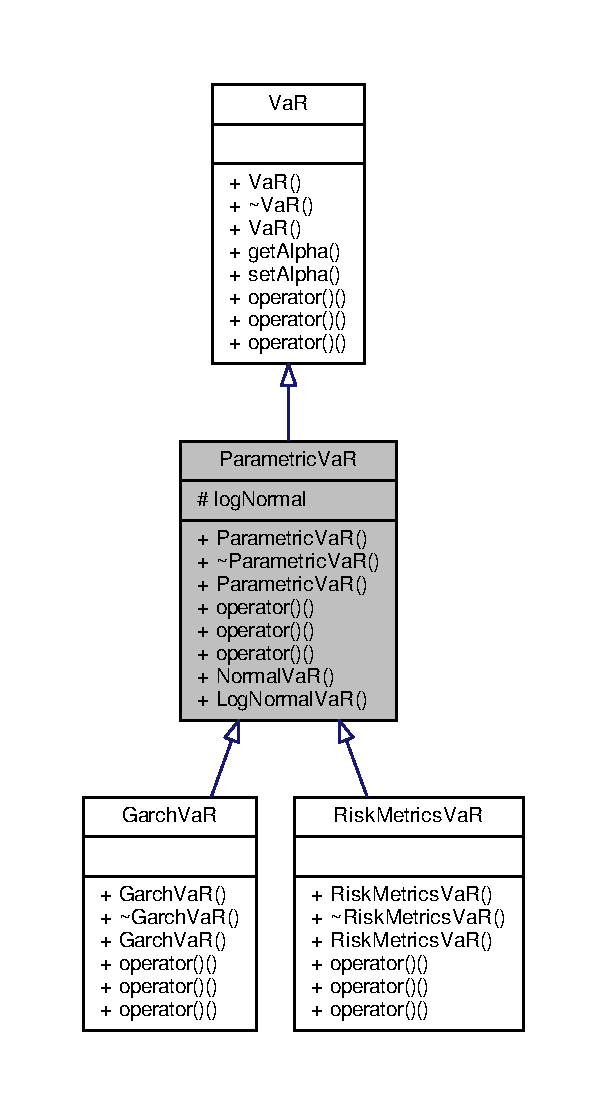
\includegraphics[width=292pt]{classParametricVaR__inherit__graph}
\end{center}
\end{figure}


Collaboration diagram for Parametric\+VaR\+:
\nopagebreak
\begin{figure}[H]
\begin{center}
\leavevmode
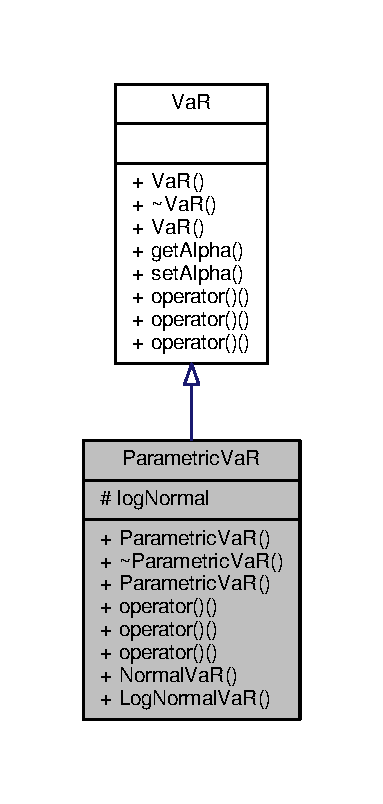
\includegraphics[width=184pt]{classParametricVaR__coll__graph}
\end{center}
\end{figure}
\subsection*{Public Member Functions}
\begin{DoxyCompactItemize}
\item 
\hyperlink{classParametricVaR_a679d72495a95d6c1be912118101a95e1}{Parametric\+VaR} (double \+\_\+alpha=.\+05, bool \+\_\+log\+Normal=false)
\item 
virtual \hyperlink{classParametricVaR_a9345f4d02e6f1facb29922d2c4be504c}{$\sim$\+Parametric\+VaR} ()
\item 
\hyperlink{classParametricVaR_aa028595da1c747f5c1887eb07157139a}{Parametric\+VaR} (const \hyperlink{classParametricVaR}{Parametric\+VaR} \&other)
\item 
virtual double \hyperlink{classParametricVaR_a54589e13bb45da786d574656eb67b5fb}{operator()} (double \+\_\+mean\+Return, double \+\_\+sigmatminus1, double \+\_\+returnt) const =0
\item 
virtual double \hyperlink{classParametricVaR_a5fda9d0e1033ff6e93dd112555ee5e0b}{operator()} (double \+\_\+mean\+Return, const \hyperlink{compute__returns__eigen_8h_a1eb6a9306ef406d7975f3cbf2e247777}{Vec} \&returns) const =0
\item 
virtual double \hyperlink{classParametricVaR_aa07f1d64aff5abf484835cd9105af9c9}{operator()} (const \hyperlink{compute__returns__eigen_8h_a1eb6a9306ef406d7975f3cbf2e247777}{Vec} \&returns) const =0
\item 
double \hyperlink{classParametricVaR_afdcc1e8748cff0a19d731f7a22c1d0c9}{Normal\+VaR} (double u, double sigma) const
\item 
double \hyperlink{classParametricVaR_aa26635a0fe04bd06580c50855360128a}{Log\+Normal\+VaR} (double u, double sigma) const
\end{DoxyCompactItemize}
\subsection*{Protected Attributes}
\begin{DoxyCompactItemize}
\item 
bool \hyperlink{classParametricVaR_a6e1dd396274079af9e1fc21068213866}{log\+Normal}
\end{DoxyCompactItemize}


\subsection{Constructor \& Destructor Documentation}
\hypertarget{classParametricVaR_a679d72495a95d6c1be912118101a95e1}{}\label{classParametricVaR_a679d72495a95d6c1be912118101a95e1} 
\index{Parametric\+VaR@{Parametric\+VaR}!Parametric\+VaR@{Parametric\+VaR}}
\index{Parametric\+VaR@{Parametric\+VaR}!Parametric\+VaR@{Parametric\+VaR}}
\subsubsection{\texorpdfstring{Parametric\+Va\+R()}{ParametricVaR()}\hspace{0.1cm}{\footnotesize\ttfamily [1/2]}}
{\footnotesize\ttfamily Parametric\+Va\+R\+::\+Parametric\+VaR (\begin{DoxyParamCaption}\item[{double}]{\+\_\+alpha = {\ttfamily .05},  }\item[{bool}]{\+\_\+log\+Normal = {\ttfamily false} }\end{DoxyParamCaption})}

\hypertarget{classParametricVaR_a9345f4d02e6f1facb29922d2c4be504c}{}\label{classParametricVaR_a9345f4d02e6f1facb29922d2c4be504c} 
\index{Parametric\+VaR@{Parametric\+VaR}!````~Parametric\+VaR@{$\sim$\+Parametric\+VaR}}
\index{````~Parametric\+VaR@{$\sim$\+Parametric\+VaR}!Parametric\+VaR@{Parametric\+VaR}}
\subsubsection{\texorpdfstring{$\sim$\+Parametric\+Va\+R()}{~ParametricVaR()}}
{\footnotesize\ttfamily virtual Parametric\+Va\+R\+::$\sim$\+Parametric\+VaR (\begin{DoxyParamCaption}{ }\end{DoxyParamCaption})\hspace{0.3cm}{\ttfamily [inline]}, {\ttfamily [virtual]}}

\hypertarget{classParametricVaR_aa028595da1c747f5c1887eb07157139a}{}\label{classParametricVaR_aa028595da1c747f5c1887eb07157139a} 
\index{Parametric\+VaR@{Parametric\+VaR}!Parametric\+VaR@{Parametric\+VaR}}
\index{Parametric\+VaR@{Parametric\+VaR}!Parametric\+VaR@{Parametric\+VaR}}
\subsubsection{\texorpdfstring{Parametric\+Va\+R()}{ParametricVaR()}\hspace{0.1cm}{\footnotesize\ttfamily [2/2]}}
{\footnotesize\ttfamily Parametric\+Va\+R\+::\+Parametric\+VaR (\begin{DoxyParamCaption}\item[{const \hyperlink{classParametricVaR}{Parametric\+VaR} \&}]{other }\end{DoxyParamCaption})}



\subsection{Member Function Documentation}
\hypertarget{classParametricVaR_aa26635a0fe04bd06580c50855360128a}{}\label{classParametricVaR_aa26635a0fe04bd06580c50855360128a} 
\index{Parametric\+VaR@{Parametric\+VaR}!Log\+Normal\+VaR@{Log\+Normal\+VaR}}
\index{Log\+Normal\+VaR@{Log\+Normal\+VaR}!Parametric\+VaR@{Parametric\+VaR}}
\subsubsection{\texorpdfstring{Log\+Normal\+Va\+R()}{LogNormalVaR()}}
{\footnotesize\ttfamily double Parametric\+Va\+R\+::\+Log\+Normal\+VaR (\begin{DoxyParamCaption}\item[{double}]{u,  }\item[{double}]{sigma }\end{DoxyParamCaption}) const}

\hypertarget{classParametricVaR_afdcc1e8748cff0a19d731f7a22c1d0c9}{}\label{classParametricVaR_afdcc1e8748cff0a19d731f7a22c1d0c9} 
\index{Parametric\+VaR@{Parametric\+VaR}!Normal\+VaR@{Normal\+VaR}}
\index{Normal\+VaR@{Normal\+VaR}!Parametric\+VaR@{Parametric\+VaR}}
\subsubsection{\texorpdfstring{Normal\+Va\+R()}{NormalVaR()}}
{\footnotesize\ttfamily double Parametric\+Va\+R\+::\+Normal\+VaR (\begin{DoxyParamCaption}\item[{double}]{u,  }\item[{double}]{sigma }\end{DoxyParamCaption}) const}

\hypertarget{classParametricVaR_a54589e13bb45da786d574656eb67b5fb}{}\label{classParametricVaR_a54589e13bb45da786d574656eb67b5fb} 
\index{Parametric\+VaR@{Parametric\+VaR}!operator()@{operator()}}
\index{operator()@{operator()}!Parametric\+VaR@{Parametric\+VaR}}
\subsubsection{\texorpdfstring{operator()()}{operator()()}\hspace{0.1cm}{\footnotesize\ttfamily [1/3]}}
{\footnotesize\ttfamily virtual double Parametric\+Va\+R\+::operator() (\begin{DoxyParamCaption}\item[{double}]{\+\_\+mean\+Return,  }\item[{double}]{\+\_\+sigmatminus1,  }\item[{double}]{\+\_\+returnt }\end{DoxyParamCaption}) const\hspace{0.3cm}{\ttfamily [pure virtual]}}



Implements \hyperlink{classVaR_a28e1a1be9e386ed4e8503e54db4033bd}{VaR}.



Implemented in \hyperlink{classGarchVaR_a6aec8c89e48d2b2f356669ed3300f456}{Garch\+VaR}, and \hyperlink{classRiskMetricsVaR_a801fc34d2327f8fffc1315a5a9aa9df1}{Risk\+Metrics\+VaR}.

\hypertarget{classParametricVaR_a5fda9d0e1033ff6e93dd112555ee5e0b}{}\label{classParametricVaR_a5fda9d0e1033ff6e93dd112555ee5e0b} 
\index{Parametric\+VaR@{Parametric\+VaR}!operator()@{operator()}}
\index{operator()@{operator()}!Parametric\+VaR@{Parametric\+VaR}}
\subsubsection{\texorpdfstring{operator()()}{operator()()}\hspace{0.1cm}{\footnotesize\ttfamily [2/3]}}
{\footnotesize\ttfamily virtual double Parametric\+Va\+R\+::operator() (\begin{DoxyParamCaption}\item[{double}]{\+\_\+mean\+Return,  }\item[{const \hyperlink{compute__returns__eigen_8h_a1eb6a9306ef406d7975f3cbf2e247777}{Vec} \&}]{returns }\end{DoxyParamCaption}) const\hspace{0.3cm}{\ttfamily [pure virtual]}}



Implements \hyperlink{classVaR_a31cb62626488715a9133679feaba31e5}{VaR}.



Implemented in \hyperlink{classGarchVaR_ab7e9583566b26a64017edbbfb63f3e89}{Garch\+VaR}, and \hyperlink{classRiskMetricsVaR_ab83bde7047dc8e501b8e8ea115cf5e7b}{Risk\+Metrics\+VaR}.

\hypertarget{classParametricVaR_aa07f1d64aff5abf484835cd9105af9c9}{}\label{classParametricVaR_aa07f1d64aff5abf484835cd9105af9c9} 
\index{Parametric\+VaR@{Parametric\+VaR}!operator()@{operator()}}
\index{operator()@{operator()}!Parametric\+VaR@{Parametric\+VaR}}
\subsubsection{\texorpdfstring{operator()()}{operator()()}\hspace{0.1cm}{\footnotesize\ttfamily [3/3]}}
{\footnotesize\ttfamily virtual double Parametric\+Va\+R\+::operator() (\begin{DoxyParamCaption}\item[{const \hyperlink{compute__returns__eigen_8h_a1eb6a9306ef406d7975f3cbf2e247777}{Vec} \&}]{returns }\end{DoxyParamCaption}) const\hspace{0.3cm}{\ttfamily [pure virtual]}}



Implements \hyperlink{classVaR_a1bd868d9953bfaeb49f5bf7d16986631}{VaR}.



Implemented in \hyperlink{classGarchVaR_ac6d01b6567a6d0629cd95be716677763}{Garch\+VaR}, and \hyperlink{classRiskMetricsVaR_a3e79a82675a93c7467451146131a2ec5}{Risk\+Metrics\+VaR}.



\subsection{Member Data Documentation}
\hypertarget{classParametricVaR_a6e1dd396274079af9e1fc21068213866}{}\label{classParametricVaR_a6e1dd396274079af9e1fc21068213866} 
\index{Parametric\+VaR@{Parametric\+VaR}!log\+Normal@{log\+Normal}}
\index{log\+Normal@{log\+Normal}!Parametric\+VaR@{Parametric\+VaR}}
\subsubsection{\texorpdfstring{log\+Normal}{logNormal}}
{\footnotesize\ttfamily bool Parametric\+Va\+R\+::log\+Normal\hspace{0.3cm}{\ttfamily [protected]}}



The documentation for this class was generated from the following file\+:\begin{DoxyCompactItemize}
\item 
\hyperlink{var__model_8h}{var\+\_\+model.\+h}\end{DoxyCompactItemize}

\hypertarget{classPath}{}\section{Path Class Reference}
\label{classPath}\index{Path@{Path}}


\hyperlink{classPath}{Path} fait tail, mean-\/reverting, commodity process ...  




{\ttfamily \#include $<$path.\+h$>$}



Inheritance diagram for Path\+:
\nopagebreak
\begin{figure}[H]
\begin{center}
\leavevmode
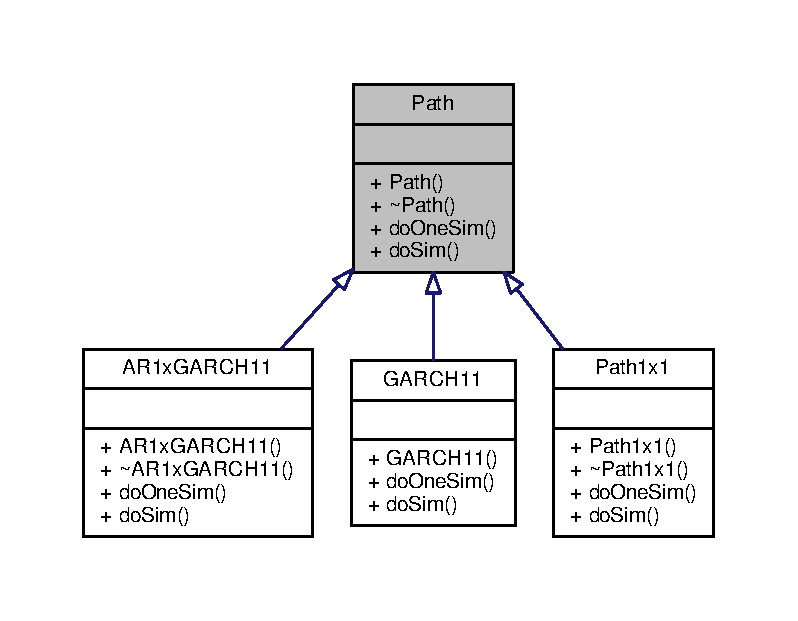
\includegraphics[width=350pt]{classPath__inherit__graph}
\end{center}
\end{figure}


Collaboration diagram for Path\+:
\nopagebreak
\begin{figure}[H]
\begin{center}
\leavevmode
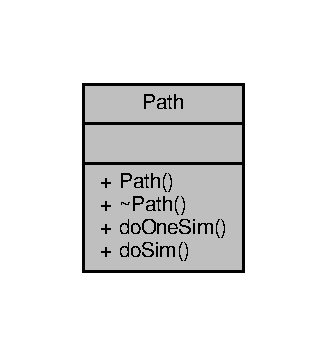
\includegraphics[width=157pt]{classPath__coll__graph}
\end{center}
\end{figure}
\subsection*{Public Member Functions}
\begin{DoxyCompactItemize}
\item 
\hyperlink{classPath_af26cfab021ddf49af73da3b2beca85ac}{Path} ()
\item 
virtual \hyperlink{classPath_a11618e66fc700531d3ad998acfdb88a3}{$\sim$\+Path} ()
\item 
virtual double \hyperlink{classPath_a6e75e5a329c48cafecd03a355f90b694}{do\+One\+Sim} (const double \&u, const double \&Sigmat, const double \&Returnt, const double \&Returntminus1) const =0
\item 
virtual Eigen\+::\+Vector\+Xd \hyperlink{classPath_a8917612a585bce52dbd52b1b643a517a}{do\+Sim} (const \hyperlink{compute__returns__eigen_8h_a1eb6a9306ef406d7975f3cbf2e247777}{Vec} \&u, const \hyperlink{compute__returns__eigen_8h_a1eb6a9306ef406d7975f3cbf2e247777}{Vec} \&Sigmat, const \hyperlink{compute__returns__eigen_8h_a1eb6a9306ef406d7975f3cbf2e247777}{Vec} \&Returnt) const =0
\end{DoxyCompactItemize}


\subsection{Detailed Description}
\hyperlink{classPath}{Path} fait tail, mean-\/reverting, commodity process ... 

\subsection{Constructor \& Destructor Documentation}
\hypertarget{classPath_af26cfab021ddf49af73da3b2beca85ac}{}\label{classPath_af26cfab021ddf49af73da3b2beca85ac} 
\index{Path@{Path}!Path@{Path}}
\index{Path@{Path}!Path@{Path}}
\subsubsection{\texorpdfstring{Path()}{Path()}}
{\footnotesize\ttfamily Path\+::\+Path (\begin{DoxyParamCaption}{ }\end{DoxyParamCaption})\hspace{0.3cm}{\ttfamily [inline]}}

\hypertarget{classPath_a11618e66fc700531d3ad998acfdb88a3}{}\label{classPath_a11618e66fc700531d3ad998acfdb88a3} 
\index{Path@{Path}!````~Path@{$\sim$\+Path}}
\index{````~Path@{$\sim$\+Path}!Path@{Path}}
\subsubsection{\texorpdfstring{$\sim$\+Path()}{~Path()}}
{\footnotesize\ttfamily virtual Path\+::$\sim$\+Path (\begin{DoxyParamCaption}{ }\end{DoxyParamCaption})\hspace{0.3cm}{\ttfamily [inline]}, {\ttfamily [virtual]}}



\subsection{Member Function Documentation}
\hypertarget{classPath_a6e75e5a329c48cafecd03a355f90b694}{}\label{classPath_a6e75e5a329c48cafecd03a355f90b694} 
\index{Path@{Path}!do\+One\+Sim@{do\+One\+Sim}}
\index{do\+One\+Sim@{do\+One\+Sim}!Path@{Path}}
\subsubsection{\texorpdfstring{do\+One\+Sim()}{doOneSim()}}
{\footnotesize\ttfamily virtual double Path\+::do\+One\+Sim (\begin{DoxyParamCaption}\item[{const double \&}]{u,  }\item[{const double \&}]{Sigmat,  }\item[{const double \&}]{Returnt,  }\item[{const double \&}]{Returntminus1 }\end{DoxyParamCaption}) const\hspace{0.3cm}{\ttfamily [pure virtual]}}



Implemented in \hyperlink{classGARCH11_a8f6e87b2b85a91e02416d4d02bf7b9ff}{G\+A\+R\+C\+H11}, \hyperlink{classAR1xGARCH11_ac30812d6e8339c48abcd5c0ce8ea0081}{A\+R1x\+G\+A\+R\+C\+H11}, and \hyperlink{classPath1x1_a522e73958cc571997153baa179b451cd}{Path1x1}.

\hypertarget{classPath_a8917612a585bce52dbd52b1b643a517a}{}\label{classPath_a8917612a585bce52dbd52b1b643a517a} 
\index{Path@{Path}!do\+Sim@{do\+Sim}}
\index{do\+Sim@{do\+Sim}!Path@{Path}}
\subsubsection{\texorpdfstring{do\+Sim()}{doSim()}}
{\footnotesize\ttfamily virtual Eigen\+::\+Vector\+Xd Path\+::do\+Sim (\begin{DoxyParamCaption}\item[{const \hyperlink{compute__returns__eigen_8h_a1eb6a9306ef406d7975f3cbf2e247777}{Vec} \&}]{u,  }\item[{const \hyperlink{compute__returns__eigen_8h_a1eb6a9306ef406d7975f3cbf2e247777}{Vec} \&}]{Sigmat,  }\item[{const \hyperlink{compute__returns__eigen_8h_a1eb6a9306ef406d7975f3cbf2e247777}{Vec} \&}]{Returnt }\end{DoxyParamCaption}) const\hspace{0.3cm}{\ttfamily [pure virtual]}}



Implemented in \hyperlink{classGARCH11_a202ee361532058114cfc036c27bef601}{G\+A\+R\+C\+H11}, \hyperlink{classAR1xGARCH11_ac97f026cefd0e8bca4bbc31100f945d7}{A\+R1x\+G\+A\+R\+C\+H11}, and \hyperlink{classPath1x1_abd21c19e5283035ebe2ca01711134e4c}{Path1x1}.



The documentation for this class was generated from the following file\+:\begin{DoxyCompactItemize}
\item 
\hyperlink{path_8h}{path.\+h}\end{DoxyCompactItemize}

\hypertarget{classPath1x1}{}\section{Path1x1 Class Reference}
\label{classPath1x1}\index{Path1x1@{Path1x1}}


{\ttfamily \#include $<$path.\+h$>$}



Inheritance diagram for Path1x1\+:
\nopagebreak
\begin{figure}[H]
\begin{center}
\leavevmode
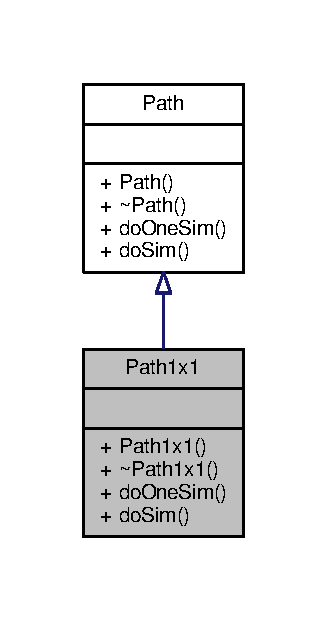
\includegraphics[width=157pt]{classPath1x1__inherit__graph}
\end{center}
\end{figure}


Collaboration diagram for Path1x1\+:
\nopagebreak
\begin{figure}[H]
\begin{center}
\leavevmode
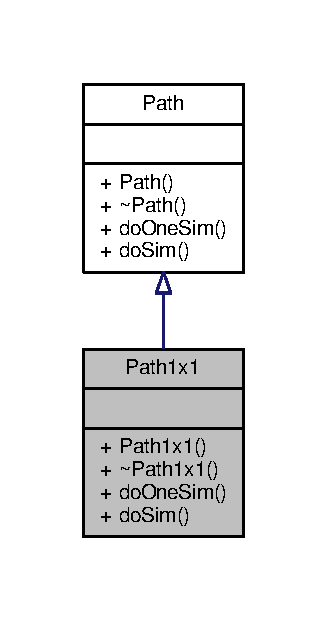
\includegraphics[width=157pt]{classPath1x1__coll__graph}
\end{center}
\end{figure}
\subsection*{Public Member Functions}
\begin{DoxyCompactItemize}
\item 
\hyperlink{classPath1x1_a4334fb2dde2817567faeb9dbdad730a4}{Path1x1} ()
\item 
virtual \hyperlink{classPath1x1_a0752d44231023e4d60403708fd8a51a5}{$\sim$\+Path1x1} ()
\item 
virtual double \hyperlink{classPath1x1_a522e73958cc571997153baa179b451cd}{do\+One\+Sim} (const double \&u, const double \&Sigmat=0., const double \&Returnt=0., const double \&Returntminus1=0.) const
\item 
virtual Eigen\+::\+Vector\+Xd \hyperlink{classPath1x1_abd21c19e5283035ebe2ca01711134e4c}{do\+Sim} (const \hyperlink{compute__returns__eigen_8h_a1eb6a9306ef406d7975f3cbf2e247777}{Vec} \&u, const \hyperlink{compute__returns__eigen_8h_a1eb6a9306ef406d7975f3cbf2e247777}{Vec} \&Sigmat=\hyperlink{compute__returns__eigen_8h_a1eb6a9306ef406d7975f3cbf2e247777}{Vec}(), const \hyperlink{compute__returns__eigen_8h_a1eb6a9306ef406d7975f3cbf2e247777}{Vec} \&Returnt=\hyperlink{compute__returns__eigen_8h_a1eb6a9306ef406d7975f3cbf2e247777}{Vec}()) const
\end{DoxyCompactItemize}


\subsection{Constructor \& Destructor Documentation}
\hypertarget{classPath1x1_a4334fb2dde2817567faeb9dbdad730a4}{}\label{classPath1x1_a4334fb2dde2817567faeb9dbdad730a4} 
\index{Path1x1@{Path1x1}!Path1x1@{Path1x1}}
\index{Path1x1@{Path1x1}!Path1x1@{Path1x1}}
\subsubsection{\texorpdfstring{Path1x1()}{Path1x1()}}
{\footnotesize\ttfamily Path1x1\+::\+Path1x1 (\begin{DoxyParamCaption}{ }\end{DoxyParamCaption})}

\hypertarget{classPath1x1_a0752d44231023e4d60403708fd8a51a5}{}\label{classPath1x1_a0752d44231023e4d60403708fd8a51a5} 
\index{Path1x1@{Path1x1}!````~Path1x1@{$\sim$\+Path1x1}}
\index{````~Path1x1@{$\sim$\+Path1x1}!Path1x1@{Path1x1}}
\subsubsection{\texorpdfstring{$\sim$\+Path1x1()}{~Path1x1()}}
{\footnotesize\ttfamily virtual Path1x1\+::$\sim$\+Path1x1 (\begin{DoxyParamCaption}{ }\end{DoxyParamCaption})\hspace{0.3cm}{\ttfamily [inline]}, {\ttfamily [virtual]}}



\subsection{Member Function Documentation}
\hypertarget{classPath1x1_a522e73958cc571997153baa179b451cd}{}\label{classPath1x1_a522e73958cc571997153baa179b451cd} 
\index{Path1x1@{Path1x1}!do\+One\+Sim@{do\+One\+Sim}}
\index{do\+One\+Sim@{do\+One\+Sim}!Path1x1@{Path1x1}}
\subsubsection{\texorpdfstring{do\+One\+Sim()}{doOneSim()}}
{\footnotesize\ttfamily virtual double Path1x1\+::do\+One\+Sim (\begin{DoxyParamCaption}\item[{const double \&}]{u,  }\item[{const double \&}]{Sigmat = {\ttfamily 0.},  }\item[{const double \&}]{Returnt = {\ttfamily 0.},  }\item[{const double \&}]{Returntminus1 = {\ttfamily 0.} }\end{DoxyParamCaption}) const\hspace{0.3cm}{\ttfamily [virtual]}}



Implements \hyperlink{classPath_a6e75e5a329c48cafecd03a355f90b694}{Path}.

\hypertarget{classPath1x1_abd21c19e5283035ebe2ca01711134e4c}{}\label{classPath1x1_abd21c19e5283035ebe2ca01711134e4c} 
\index{Path1x1@{Path1x1}!do\+Sim@{do\+Sim}}
\index{do\+Sim@{do\+Sim}!Path1x1@{Path1x1}}
\subsubsection{\texorpdfstring{do\+Sim()}{doSim()}}
{\footnotesize\ttfamily virtual Eigen\+::\+Vector\+Xd Path1x1\+::do\+Sim (\begin{DoxyParamCaption}\item[{const \hyperlink{compute__returns__eigen_8h_a1eb6a9306ef406d7975f3cbf2e247777}{Vec} \&}]{u,  }\item[{const \hyperlink{compute__returns__eigen_8h_a1eb6a9306ef406d7975f3cbf2e247777}{Vec} \&}]{Sigmat = {\ttfamily \hyperlink{compute__returns__eigen_8h_a1eb6a9306ef406d7975f3cbf2e247777}{Vec}()},  }\item[{const \hyperlink{compute__returns__eigen_8h_a1eb6a9306ef406d7975f3cbf2e247777}{Vec} \&}]{Returnt = {\ttfamily \hyperlink{compute__returns__eigen_8h_a1eb6a9306ef406d7975f3cbf2e247777}{Vec}()} }\end{DoxyParamCaption}) const\hspace{0.3cm}{\ttfamily [virtual]}}



Implements \hyperlink{classPath_a8917612a585bce52dbd52b1b643a517a}{Path}.



The documentation for this class was generated from the following file\+:\begin{DoxyCompactItemize}
\item 
\hyperlink{path_8h}{path.\+h}\end{DoxyCompactItemize}

\hypertarget{classPca}{}\section{Pca Class Reference}
\label{classPca}\index{Pca@{Pca}}


{\ttfamily \#include $<$pca.\+h$>$}



Collaboration diagram for Pca\+:
\nopagebreak
\begin{figure}[H]
\begin{center}
\leavevmode
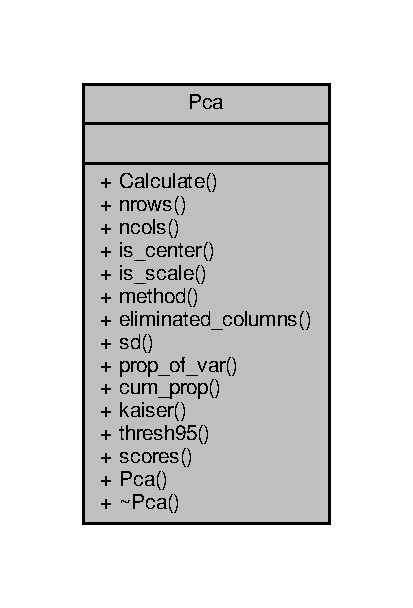
\includegraphics[width=198pt]{classPca__coll__graph}
\end{center}
\end{figure}
\subsection*{Public Member Functions}
\begin{DoxyCompactItemize}
\item 
int \hyperlink{classPca_a69bab38091166e75c71a20952c4c9ef4}{Calculate} (std\+::vector$<$ float $>$ \&x, const unsigned int \&\hyperlink{classPca_a1de7db7c35c005e7920dd95579ae820b}{nrows}, const unsigned int \&\hyperlink{classPca_ab3e3ef5de29c495ad8b8ad7ed0ae2bbe}{ncols}, const bool is\+\_\+corr=true, const bool \hyperlink{classPca_a756656415dc43a2a68f4394f719351b2}{is\+\_\+center}=true, const bool \hyperlink{classPca_acf41e5dccf22ba87069b3eb1bc586307}{is\+\_\+scale}=true)
\begin{DoxyCompactList}\small\item\em Initializing values and performing P\+CA. \end{DoxyCompactList}\item 
unsigned int \hyperlink{classPca_a1de7db7c35c005e7920dd95579ae820b}{nrows} (void)
\begin{DoxyCompactList}\small\item\em Return number of rows in initial matrix. \end{DoxyCompactList}\item 
unsigned int \hyperlink{classPca_ab3e3ef5de29c495ad8b8ad7ed0ae2bbe}{ncols} (void)
\begin{DoxyCompactList}\small\item\em Return number of cols in initial matrix. \end{DoxyCompactList}\item 
bool \hyperlink{classPca_a756656415dc43a2a68f4394f719351b2}{is\+\_\+center} (void)
\begin{DoxyCompactList}\small\item\em If variables are centered. \end{DoxyCompactList}\item 
bool \hyperlink{classPca_acf41e5dccf22ba87069b3eb1bc586307}{is\+\_\+scale} (void)
\begin{DoxyCompactList}\small\item\em If variables are scaled. \end{DoxyCompactList}\item 
std\+::string \hyperlink{classPca_aecaeb63b64fe48f9307ee89075ed6929}{method} (void)
\begin{DoxyCompactList}\small\item\em Method for calculation of principal components. \end{DoxyCompactList}\item 
std\+::vector$<$ unsigned int $>$ \hyperlink{classPca_a846bfe6726f3c846a50ec045567d3861}{eliminated\+\_\+columns} (void)
\begin{DoxyCompactList}\small\item\em Returns numbers of eliminated columns. \end{DoxyCompactList}\item 
std\+::vector$<$ float $>$ \hyperlink{classPca_a687a02cd667152bc5ce9de328519799b}{sd} (void)
\begin{DoxyCompactList}\small\item\em Standard deviation of each principal component. \end{DoxyCompactList}\item 
std\+::vector$<$ float $>$ \hyperlink{classPca_a70f5508f41d2d61464fe8ce21f48dc89}{prop\+\_\+of\+\_\+var} (void)
\begin{DoxyCompactList}\small\item\em Proportion of variance. \end{DoxyCompactList}\item 
std\+::vector$<$ float $>$ \hyperlink{classPca_a08407cc5449d7461b1b1b828c464e80a}{cum\+\_\+prop} (void)
\begin{DoxyCompactList}\small\item\em Cumulative proportion. \end{DoxyCompactList}\item 
unsigned int \hyperlink{classPca_a6c1fbe858a4cde8aa34cab8c19c84941}{kaiser} (void)
\begin{DoxyCompactList}\small\item\em Principal component by the Kaiser criterion. \end{DoxyCompactList}\item 
unsigned int \hyperlink{classPca_a0ff511b4a419122a8ac6db494289ae2a}{thresh95} (void)
\begin{DoxyCompactList}\small\item\em 95\% threshold \end{DoxyCompactList}\item 
std\+::vector$<$ float $>$ \hyperlink{classPca_a469f69a53d76c2f7ad26e28e969bd09c}{scores} (void)
\begin{DoxyCompactList}\small\item\em Rotated values (scores) \end{DoxyCompactList}\item 
\hyperlink{classPca_ac8f42fb6ce69fb1a3a85c99d6b49204c}{Pca} (void)
\begin{DoxyCompactList}\small\item\em Class constructor. \end{DoxyCompactList}\item 
\hyperlink{classPca_a900858e8760079d51bff8fd267f551ce}{$\sim$\+Pca} (void)
\begin{DoxyCompactList}\small\item\em Class destructor. \end{DoxyCompactList}\end{DoxyCompactItemize}


\subsection{Constructor \& Destructor Documentation}
\hypertarget{classPca_ac8f42fb6ce69fb1a3a85c99d6b49204c}{}\label{classPca_ac8f42fb6ce69fb1a3a85c99d6b49204c} 
\index{Pca@{Pca}!Pca@{Pca}}
\index{Pca@{Pca}!Pca@{Pca}}
\subsubsection{\texorpdfstring{Pca()}{Pca()}}
{\footnotesize\ttfamily Pca\+::\+Pca (\begin{DoxyParamCaption}\item[{void}]{ }\end{DoxyParamCaption})}



Class constructor. 

\hypertarget{classPca_a900858e8760079d51bff8fd267f551ce}{}\label{classPca_a900858e8760079d51bff8fd267f551ce} 
\index{Pca@{Pca}!````~Pca@{$\sim$\+Pca}}
\index{````~Pca@{$\sim$\+Pca}!Pca@{Pca}}
\subsubsection{\texorpdfstring{$\sim$\+Pca()}{~Pca()}}
{\footnotesize\ttfamily Pca\+::$\sim$\+Pca (\begin{DoxyParamCaption}\item[{void}]{ }\end{DoxyParamCaption})}



Class destructor. 



\subsection{Member Function Documentation}
\hypertarget{classPca_a69bab38091166e75c71a20952c4c9ef4}{}\label{classPca_a69bab38091166e75c71a20952c4c9ef4} 
\index{Pca@{Pca}!Calculate@{Calculate}}
\index{Calculate@{Calculate}!Pca@{Pca}}
\subsubsection{\texorpdfstring{Calculate()}{Calculate()}}
{\footnotesize\ttfamily int Pca\+::\+Calculate (\begin{DoxyParamCaption}\item[{std\+::vector$<$ float $>$ \&}]{x,  }\item[{const unsigned int \&}]{nrows,  }\item[{const unsigned int \&}]{ncols,  }\item[{const bool}]{is\+\_\+corr = {\ttfamily true},  }\item[{const bool}]{is\+\_\+center = {\ttfamily true},  }\item[{const bool}]{is\+\_\+scale = {\ttfamily true} }\end{DoxyParamCaption})}



Initializing values and performing P\+CA. 

The main method for performin Principal Component Analysis 
\begin{DoxyParams}{Parameters}
{\em x} & Initial data matrix \\
\hline
{\em nrows} & Number of matrix rows \\
\hline
{\em ncols} & Number of matrix cols \\
\hline
{\em is\+\_\+corr} & Correlation matrix will be used instead of covariance matrix \\
\hline
{\em is\+\_\+center} & Whether the variables should be shifted to be zero centered \\
\hline
{\em is\+\_\+scale} & Whether the variables should be scaled to have unit variance \\
\hline
\end{DoxyParams}
\begin{DoxyReturn}{Returns}
0 if everything is Ok -\/1 if there were some errors 
\end{DoxyReturn}
\hypertarget{classPca_a08407cc5449d7461b1b1b828c464e80a}{}\label{classPca_a08407cc5449d7461b1b1b828c464e80a} 
\index{Pca@{Pca}!cum\+\_\+prop@{cum\+\_\+prop}}
\index{cum\+\_\+prop@{cum\+\_\+prop}!Pca@{Pca}}
\subsubsection{\texorpdfstring{cum\+\_\+prop()}{cum\_prop()}}
{\footnotesize\ttfamily std\+::vector$<$float$>$ Pca\+::cum\+\_\+prop (\begin{DoxyParamCaption}\item[{void}]{ }\end{DoxyParamCaption})}



Cumulative proportion. 

\begin{DoxyReturn}{Returns}
Vector of cumulative proportions for each components 
\end{DoxyReturn}
\hypertarget{classPca_a846bfe6726f3c846a50ec045567d3861}{}\label{classPca_a846bfe6726f3c846a50ec045567d3861} 
\index{Pca@{Pca}!eliminated\+\_\+columns@{eliminated\+\_\+columns}}
\index{eliminated\+\_\+columns@{eliminated\+\_\+columns}!Pca@{Pca}}
\subsubsection{\texorpdfstring{eliminated\+\_\+columns()}{eliminated\_columns()}}
{\footnotesize\ttfamily std\+::vector$<$unsigned int$>$ Pca\+::eliminated\+\_\+columns (\begin{DoxyParamCaption}\item[{void}]{ }\end{DoxyParamCaption})}



Returns numbers of eliminated columns. 

If standard deviation of a column is equal to 0, the column shoud be rejected, or P\+CA will fail. \begin{DoxyReturn}{Returns}
Numbers of eliminated columns, empty vector otherwise 
\end{DoxyReturn}
\hypertarget{classPca_a756656415dc43a2a68f4394f719351b2}{}\label{classPca_a756656415dc43a2a68f4394f719351b2} 
\index{Pca@{Pca}!is\+\_\+center@{is\+\_\+center}}
\index{is\+\_\+center@{is\+\_\+center}!Pca@{Pca}}
\subsubsection{\texorpdfstring{is\+\_\+center()}{is\_center()}}
{\footnotesize\ttfamily bool Pca\+::is\+\_\+center (\begin{DoxyParamCaption}\item[{void}]{ }\end{DoxyParamCaption})}



If variables are centered. 

\begin{DoxyReturn}{Returns}
true -\/ variables are centered false -\/ otherwise 
\end{DoxyReturn}
\hypertarget{classPca_acf41e5dccf22ba87069b3eb1bc586307}{}\label{classPca_acf41e5dccf22ba87069b3eb1bc586307} 
\index{Pca@{Pca}!is\+\_\+scale@{is\+\_\+scale}}
\index{is\+\_\+scale@{is\+\_\+scale}!Pca@{Pca}}
\subsubsection{\texorpdfstring{is\+\_\+scale()}{is\_scale()}}
{\footnotesize\ttfamily bool Pca\+::is\+\_\+scale (\begin{DoxyParamCaption}\item[{void}]{ }\end{DoxyParamCaption})}



If variables are scaled. 

\begin{DoxyReturn}{Returns}
true -\/ variables are scaled false -\/ otherwise 
\end{DoxyReturn}
\hypertarget{classPca_a6c1fbe858a4cde8aa34cab8c19c84941}{}\label{classPca_a6c1fbe858a4cde8aa34cab8c19c84941} 
\index{Pca@{Pca}!kaiser@{kaiser}}
\index{kaiser@{kaiser}!Pca@{Pca}}
\subsubsection{\texorpdfstring{kaiser()}{kaiser()}}
{\footnotesize\ttfamily unsigned int Pca\+::kaiser (\begin{DoxyParamCaption}\item[{void}]{ }\end{DoxyParamCaption})}



Principal component by the Kaiser criterion. 

Number of the last component with eigenvalue greater than 1. \begin{DoxyReturn}{Returns}
Number of the first components we should retain defined by the Kaiser criterion 
\end{DoxyReturn}
\hypertarget{classPca_aecaeb63b64fe48f9307ee89075ed6929}{}\label{classPca_aecaeb63b64fe48f9307ee89075ed6929} 
\index{Pca@{Pca}!method@{method}}
\index{method@{method}!Pca@{Pca}}
\subsubsection{\texorpdfstring{method()}{method()}}
{\footnotesize\ttfamily std\+::string Pca\+::method (\begin{DoxyParamCaption}\item[{void}]{ }\end{DoxyParamCaption})}



Method for calculation of principal components. 

There are different methods used. The most used is S\+VD. But in some cases it may be correlation or covariance matrices. If \begin{DoxyReturn}{Returns}
\char`\"{}svd\char`\"{} -\/ P\+CA with singular value decomposition \char`\"{}cor\char`\"{} -\/ P\+CA with correlation matrix \char`\"{}cov\char`\"{} -\/ P\+CA with covariance matrix 
\end{DoxyReturn}
\hypertarget{classPca_ab3e3ef5de29c495ad8b8ad7ed0ae2bbe}{}\label{classPca_ab3e3ef5de29c495ad8b8ad7ed0ae2bbe} 
\index{Pca@{Pca}!ncols@{ncols}}
\index{ncols@{ncols}!Pca@{Pca}}
\subsubsection{\texorpdfstring{ncols()}{ncols()}}
{\footnotesize\ttfamily unsigned int Pca\+::ncols (\begin{DoxyParamCaption}\item[{void}]{ }\end{DoxyParamCaption})}



Return number of cols in initial matrix. 

\begin{DoxyReturn}{Returns}
Number of cols in initial matrix 
\end{DoxyReturn}
\hypertarget{classPca_a1de7db7c35c005e7920dd95579ae820b}{}\label{classPca_a1de7db7c35c005e7920dd95579ae820b} 
\index{Pca@{Pca}!nrows@{nrows}}
\index{nrows@{nrows}!Pca@{Pca}}
\subsubsection{\texorpdfstring{nrows()}{nrows()}}
{\footnotesize\ttfamily unsigned int Pca\+::nrows (\begin{DoxyParamCaption}\item[{void}]{ }\end{DoxyParamCaption})}



Return number of rows in initial matrix. 

\begin{DoxyReturn}{Returns}
Number of rows in initial matrix 
\end{DoxyReturn}
\hypertarget{classPca_a70f5508f41d2d61464fe8ce21f48dc89}{}\label{classPca_a70f5508f41d2d61464fe8ce21f48dc89} 
\index{Pca@{Pca}!prop\+\_\+of\+\_\+var@{prop\+\_\+of\+\_\+var}}
\index{prop\+\_\+of\+\_\+var@{prop\+\_\+of\+\_\+var}!Pca@{Pca}}
\subsubsection{\texorpdfstring{prop\+\_\+of\+\_\+var()}{prop\_of\_var()}}
{\footnotesize\ttfamily std\+::vector$<$float$>$ Pca\+::prop\+\_\+of\+\_\+var (\begin{DoxyParamCaption}\item[{void}]{ }\end{DoxyParamCaption})}



Proportion of variance. 

\begin{DoxyReturn}{Returns}
Vector of variances for each component 
\end{DoxyReturn}
\hypertarget{classPca_a469f69a53d76c2f7ad26e28e969bd09c}{}\label{classPca_a469f69a53d76c2f7ad26e28e969bd09c} 
\index{Pca@{Pca}!scores@{scores}}
\index{scores@{scores}!Pca@{Pca}}
\subsubsection{\texorpdfstring{scores()}{scores()}}
{\footnotesize\ttfamily std\+::vector$<$float$>$ Pca\+::scores (\begin{DoxyParamCaption}\item[{void}]{ }\end{DoxyParamCaption})}



Rotated values (scores) 

Return calculated scores (coordinates in a new space) as vector. Matrix filled by rows. \begin{DoxyReturn}{Returns}
Vector of scores 
\end{DoxyReturn}
\hypertarget{classPca_a687a02cd667152bc5ce9de328519799b}{}\label{classPca_a687a02cd667152bc5ce9de328519799b} 
\index{Pca@{Pca}!sd@{sd}}
\index{sd@{sd}!Pca@{Pca}}
\subsubsection{\texorpdfstring{sd()}{sd()}}
{\footnotesize\ttfamily std\+::vector$<$float$>$ Pca\+::sd (\begin{DoxyParamCaption}\item[{void}]{ }\end{DoxyParamCaption})}



Standard deviation of each principal component. 

\begin{DoxyReturn}{Returns}
Vector of standard deviation for each principal component\+: 1st element is sd for 1st PC, 2nd -\/ for 2nd PC and so on. 
\end{DoxyReturn}
\hypertarget{classPca_a0ff511b4a419122a8ac6db494289ae2a}{}\label{classPca_a0ff511b4a419122a8ac6db494289ae2a} 
\index{Pca@{Pca}!thresh95@{thresh95}}
\index{thresh95@{thresh95}!Pca@{Pca}}
\subsubsection{\texorpdfstring{thresh95()}{thresh95()}}
{\footnotesize\ttfamily unsigned int Pca\+::thresh95 (\begin{DoxyParamCaption}\item[{void}]{ }\end{DoxyParamCaption})}



95\% threshold 

Retain only PC which cumulative proportion is less than 0.\+95 \begin{DoxyReturn}{Returns}
Number of P\+Cs should be retain with the 95\% threshold criterion 
\end{DoxyReturn}


The documentation for this class was generated from the following file\+:\begin{DoxyCompactItemize}
\item 
\hyperlink{pca_8h}{pca.\+h}\end{DoxyCompactItemize}

\hypertarget{classPortfolio}{}\section{Portfolio Class Reference}
\label{classPortfolio}\index{Portfolio@{Portfolio}}


{\ttfamily \#include $<$portfolio.\+h$>$}



Collaboration diagram for Portfolio\+:
\nopagebreak
\begin{figure}[H]
\begin{center}
\leavevmode
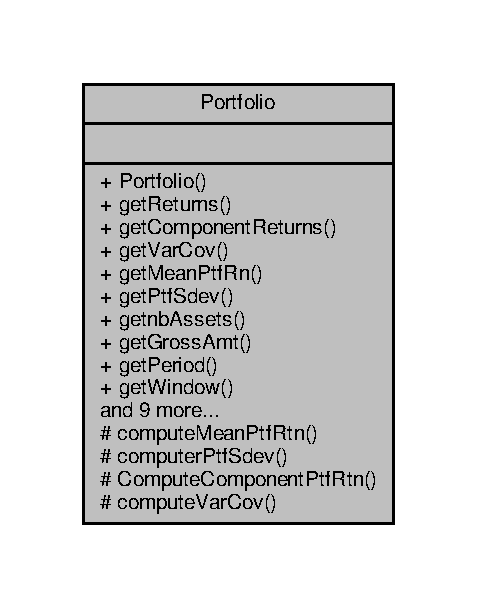
\includegraphics[width=229pt]{classPortfolio__coll__graph}
\end{center}
\end{figure}
\subsection*{Public Member Functions}
\begin{DoxyCompactItemize}
\item 
\hyperlink{classPortfolio_a573528cf895e6c963c37f423486aaac9}{Portfolio} (const \hyperlink{portfolio_8h_ab6c2cd0942dd9f72ca64d9dbadb0df64}{Ptf} \&\+\_\+ptf, const \hyperlink{compute__returns__eigen_8h_a1eb6a9306ef406d7975f3cbf2e247777}{Vec} \&\+\_\+weights, shared\+\_\+ptr$<$ \hyperlink{classComputeReturn}{Compute\+Return} $>$ \&\+\_\+cr, bool \+\_\+is\+FI=false, double \+\_\+gross\+Notional=1.)
\item 
\hyperlink{compute__returns__eigen_8h_a1eb6a9306ef406d7975f3cbf2e247777}{Vec} \hyperlink{classPortfolio_a51b835c644d10dcad9af190112d89123}{get\+Returns} (size\+\_\+t p=0) const
\item 
\hyperlink{compute__returns__eigen_8h_a1eb6a9306ef406d7975f3cbf2e247777}{Vec} \hyperlink{classPortfolio_aa235d5de98468ec656ddff1550fe5fbf}{get\+Component\+Returns} (size\+\_\+t p) const
\item 
Eigen\+::\+Matrix\+Xd \hyperlink{classPortfolio_adc5f7b744cacda38f442277d60ab77a0}{get\+Var\+Cov} () const
\item 
double \hyperlink{classPortfolio_a391b4742d7394009c34e9c9e4addc35e}{get\+Mean\+Ptf\+Rn} () const
\item 
double \hyperlink{classPortfolio_a4483f32cc7d592016c04acc7500e8217}{get\+Ptf\+Sdev} () const
\item 
double \hyperlink{classPortfolio_a165529ad0f08f24081e3bca8b354e217}{getnb\+Assets} () const
\item 
double \hyperlink{classPortfolio_aa91be98ef8fdd16bd3ebc9aa66529554}{get\+Gross\+Amt} () const
\item 
unsigned int \hyperlink{classPortfolio_a86ea8204e8ba0c9dd69c0fd3ba4abb16}{get\+Period} () const
\item 
unsigned int \hyperlink{classPortfolio_a3d2bbcfa8f794d8fefad630abefdce7b}{get\+Window} () const
\item 
bool \hyperlink{classPortfolio_acdfc56639cad8ed648780d81f066d760}{is\+Fixed\+Income} () const
\item 
\hyperlink{portfolio_8h_ab6c2cd0942dd9f72ca64d9dbadb0df64}{Ptf} \hyperlink{classPortfolio_a28f00509ec2ed08fe781eb684c923348}{get\+Positions} () const
\item 
void \hyperlink{classPortfolio_aa00669a3d5caece170ee8b28c0c67a2d}{compute\+Rtn} (unsigned int nb\+Assets)
\item 
\hyperlink{compute__returns__eigen_8h_a1eb6a9306ef406d7975f3cbf2e247777}{Vec} \hyperlink{classPortfolio_a539d00aaacb83cb6b7ed8862db277a0b}{get\+Compute\+Return\+Std\+Dev} (size\+\_\+t p=0) const
\begin{DoxyCompactList}\small\item\em Compute rolling std dev for component return p. \end{DoxyCompactList}\item 
\hyperlink{compute__returns__eigen_8h_a1eb6a9306ef406d7975f3cbf2e247777}{Vec} \hyperlink{classPortfolio_a336d14aaf3bbf9adfe458df6d6b97ce0}{get\+Rolling\+Mean} (size\+\_\+t p=0) const
\begin{DoxyCompactList}\small\item\em Compute rolling mean rtnaccording to period ie day, week, month and window. \end{DoxyCompactList}\item 
\hyperlink{compute__returns__eigen_8h_a1eb6a9306ef406d7975f3cbf2e247777}{Vec} \hyperlink{classPortfolio_a9833a33a238b2416e7c2c4f19ff7be8e}{get\+Rolling\+Std\+Dev} (size\+\_\+t p=0) const
\begin{DoxyCompactList}\small\item\em // Compute rolling std dev according to period ie day, week, month and window \end{DoxyCompactList}\item 
\hyperlink{compute__returns__eigen_8h_a1eb6a9306ef406d7975f3cbf2e247777}{Vec} \hyperlink{classPortfolio_a93c955e745cf06b58f1ce7c7e6fe41e5}{get\+Weight} () const
\item 
void \hyperlink{classPortfolio_a0c05f8c7ae8bd78971524ed06a98deba}{set\+Weight} (const \hyperlink{compute__returns__eigen_8h_a1eb6a9306ef406d7975f3cbf2e247777}{Vec} \&\+\_\+weights)
\item 
void \hyperlink{classPortfolio_a9458c66e10d7a6b8c037ad3584a1e70c}{set\+Returns} (const \hyperlink{compute__returns__eigen_8h_ae14dd28696f743e067dbd2594616bad6}{Mat} \&\+\_\+m\+Asset\+Returns)
\end{DoxyCompactItemize}
\subsection*{Protected Member Functions}
\begin{DoxyCompactItemize}
\item 
void \hyperlink{classPortfolio_ad2732b083b90ecd08e5bf26fb38a1834}{compute\+Mean\+Ptf\+Rtn} ()
\begin{DoxyCompactList}\small\item\em w\textquotesingle{} $\ast$ R -\/ Need to account for approx of asset return \+: delta, gamma, etc \end{DoxyCompactList}\item 
void \hyperlink{classPortfolio_aeaba88f92093501fb98c60c83b600529}{computer\+Ptf\+Sdev} ()
\begin{DoxyCompactList}\small\item\em w\textquotesingle{} $\ast$ sigma $\ast$ w -\/ Need to account for approx of asset return \+: delta, gamma, etc \end{DoxyCompactList}\item 
void \hyperlink{classPortfolio_a2824877890ad51d9261935002a6d25c0}{Compute\+Component\+Ptf\+Rtn} ()
\item 
void \hyperlink{classPortfolio_a56baf8410ef9a0c450e5fa558ac4254f}{compute\+Var\+Cov} ()
\end{DoxyCompactItemize}
\subsection*{Friends}
\begin{DoxyCompactItemize}
\item 
class \hyperlink{classPortfolio_a6135a57a82e989f986dd94c3175bc07d}{Va\+R\+Ptf\+Compute}
\end{DoxyCompactItemize}


\subsection{Constructor \& Destructor Documentation}
\hypertarget{classPortfolio_a573528cf895e6c963c37f423486aaac9}{}\label{classPortfolio_a573528cf895e6c963c37f423486aaac9} 
\index{Portfolio@{Portfolio}!Portfolio@{Portfolio}}
\index{Portfolio@{Portfolio}!Portfolio@{Portfolio}}
\subsubsection{\texorpdfstring{Portfolio()}{Portfolio()}}
{\footnotesize\ttfamily Portfolio\+::\+Portfolio (\begin{DoxyParamCaption}\item[{const \hyperlink{portfolio_8h_ab6c2cd0942dd9f72ca64d9dbadb0df64}{Ptf} \&}]{\+\_\+ptf,  }\item[{const \hyperlink{compute__returns__eigen_8h_a1eb6a9306ef406d7975f3cbf2e247777}{Vec} \&}]{\+\_\+weights,  }\item[{shared\+\_\+ptr$<$ \hyperlink{classComputeReturn}{Compute\+Return} $>$ \&}]{\+\_\+cr,  }\item[{bool}]{\+\_\+is\+FI = {\ttfamily false},  }\item[{double}]{\+\_\+gross\+Notional = {\ttfamily 1.} }\end{DoxyParamCaption})}



\subsection{Member Function Documentation}
\hypertarget{classPortfolio_a2824877890ad51d9261935002a6d25c0}{}\label{classPortfolio_a2824877890ad51d9261935002a6d25c0} 
\index{Portfolio@{Portfolio}!Compute\+Component\+Ptf\+Rtn@{Compute\+Component\+Ptf\+Rtn}}
\index{Compute\+Component\+Ptf\+Rtn@{Compute\+Component\+Ptf\+Rtn}!Portfolio@{Portfolio}}
\subsubsection{\texorpdfstring{Compute\+Component\+Ptf\+Rtn()}{ComputeComponentPtfRtn()}}
{\footnotesize\ttfamily void Portfolio\+::\+Compute\+Component\+Ptf\+Rtn (\begin{DoxyParamCaption}{ }\end{DoxyParamCaption})\hspace{0.3cm}{\ttfamily [inline]}, {\ttfamily [protected]}}

\begin{DoxyReturn}{Returns}
component ptf return 
\end{DoxyReturn}
\hypertarget{classPortfolio_ad2732b083b90ecd08e5bf26fb38a1834}{}\label{classPortfolio_ad2732b083b90ecd08e5bf26fb38a1834} 
\index{Portfolio@{Portfolio}!compute\+Mean\+Ptf\+Rtn@{compute\+Mean\+Ptf\+Rtn}}
\index{compute\+Mean\+Ptf\+Rtn@{compute\+Mean\+Ptf\+Rtn}!Portfolio@{Portfolio}}
\subsubsection{\texorpdfstring{compute\+Mean\+Ptf\+Rtn()}{computeMeanPtfRtn()}}
{\footnotesize\ttfamily void Portfolio\+::compute\+Mean\+Ptf\+Rtn (\begin{DoxyParamCaption}{ }\end{DoxyParamCaption})\hspace{0.3cm}{\ttfamily [inline]}, {\ttfamily [protected]}}



w\textquotesingle{} $\ast$ R -\/ Need to account for approx of asset return \+: delta, gamma, etc 

\hypertarget{classPortfolio_aeaba88f92093501fb98c60c83b600529}{}\label{classPortfolio_aeaba88f92093501fb98c60c83b600529} 
\index{Portfolio@{Portfolio}!computer\+Ptf\+Sdev@{computer\+Ptf\+Sdev}}
\index{computer\+Ptf\+Sdev@{computer\+Ptf\+Sdev}!Portfolio@{Portfolio}}
\subsubsection{\texorpdfstring{computer\+Ptf\+Sdev()}{computerPtfSdev()}}
{\footnotesize\ttfamily void Portfolio\+::computer\+Ptf\+Sdev (\begin{DoxyParamCaption}{ }\end{DoxyParamCaption})\hspace{0.3cm}{\ttfamily [inline]}, {\ttfamily [protected]}}



w\textquotesingle{} $\ast$ sigma $\ast$ w -\/ Need to account for approx of asset return \+: delta, gamma, etc 

\hypertarget{classPortfolio_aa00669a3d5caece170ee8b28c0c67a2d}{}\label{classPortfolio_aa00669a3d5caece170ee8b28c0c67a2d} 
\index{Portfolio@{Portfolio}!compute\+Rtn@{compute\+Rtn}}
\index{compute\+Rtn@{compute\+Rtn}!Portfolio@{Portfolio}}
\subsubsection{\texorpdfstring{compute\+Rtn()}{computeRtn()}}
{\footnotesize\ttfamily void Portfolio\+::compute\+Rtn (\begin{DoxyParamCaption}\item[{unsigned int}]{nb\+Assets }\end{DoxyParamCaption})}

\hypertarget{classPortfolio_a56baf8410ef9a0c450e5fa558ac4254f}{}\label{classPortfolio_a56baf8410ef9a0c450e5fa558ac4254f} 
\index{Portfolio@{Portfolio}!compute\+Var\+Cov@{compute\+Var\+Cov}}
\index{compute\+Var\+Cov@{compute\+Var\+Cov}!Portfolio@{Portfolio}}
\subsubsection{\texorpdfstring{compute\+Var\+Cov()}{computeVarCov()}}
{\footnotesize\ttfamily void Portfolio\+::compute\+Var\+Cov (\begin{DoxyParamCaption}{ }\end{DoxyParamCaption})\hspace{0.3cm}{\ttfamily [inline]}, {\ttfamily [protected]}}

\hypertarget{classPortfolio_aa235d5de98468ec656ddff1550fe5fbf}{}\label{classPortfolio_aa235d5de98468ec656ddff1550fe5fbf} 
\index{Portfolio@{Portfolio}!get\+Component\+Returns@{get\+Component\+Returns}}
\index{get\+Component\+Returns@{get\+Component\+Returns}!Portfolio@{Portfolio}}
\subsubsection{\texorpdfstring{get\+Component\+Returns()}{getComponentReturns()}}
{\footnotesize\ttfamily \hyperlink{compute__returns__eigen_8h_a1eb6a9306ef406d7975f3cbf2e247777}{Vec} Portfolio\+::get\+Component\+Returns (\begin{DoxyParamCaption}\item[{size\+\_\+t}]{p }\end{DoxyParamCaption}) const}

\hypertarget{classPortfolio_a539d00aaacb83cb6b7ed8862db277a0b}{}\label{classPortfolio_a539d00aaacb83cb6b7ed8862db277a0b} 
\index{Portfolio@{Portfolio}!get\+Compute\+Return\+Std\+Dev@{get\+Compute\+Return\+Std\+Dev}}
\index{get\+Compute\+Return\+Std\+Dev@{get\+Compute\+Return\+Std\+Dev}!Portfolio@{Portfolio}}
\subsubsection{\texorpdfstring{get\+Compute\+Return\+Std\+Dev()}{getComputeReturnStdDev()}}
{\footnotesize\ttfamily \hyperlink{compute__returns__eigen_8h_a1eb6a9306ef406d7975f3cbf2e247777}{Vec} Portfolio\+::get\+Compute\+Return\+Std\+Dev (\begin{DoxyParamCaption}\item[{size\+\_\+t}]{p = {\ttfamily 0} }\end{DoxyParamCaption}) const}



Compute rolling std dev for component return p. 

\hypertarget{classPortfolio_aa91be98ef8fdd16bd3ebc9aa66529554}{}\label{classPortfolio_aa91be98ef8fdd16bd3ebc9aa66529554} 
\index{Portfolio@{Portfolio}!get\+Gross\+Amt@{get\+Gross\+Amt}}
\index{get\+Gross\+Amt@{get\+Gross\+Amt}!Portfolio@{Portfolio}}
\subsubsection{\texorpdfstring{get\+Gross\+Amt()}{getGrossAmt()}}
{\footnotesize\ttfamily double Portfolio\+::get\+Gross\+Amt (\begin{DoxyParamCaption}{ }\end{DoxyParamCaption}) const\hspace{0.3cm}{\ttfamily [inline]}}

\hypertarget{classPortfolio_a391b4742d7394009c34e9c9e4addc35e}{}\label{classPortfolio_a391b4742d7394009c34e9c9e4addc35e} 
\index{Portfolio@{Portfolio}!get\+Mean\+Ptf\+Rn@{get\+Mean\+Ptf\+Rn}}
\index{get\+Mean\+Ptf\+Rn@{get\+Mean\+Ptf\+Rn}!Portfolio@{Portfolio}}
\subsubsection{\texorpdfstring{get\+Mean\+Ptf\+Rn()}{getMeanPtfRn()}}
{\footnotesize\ttfamily double Portfolio\+::get\+Mean\+Ptf\+Rn (\begin{DoxyParamCaption}{ }\end{DoxyParamCaption}) const\hspace{0.3cm}{\ttfamily [inline]}}

\hypertarget{classPortfolio_a165529ad0f08f24081e3bca8b354e217}{}\label{classPortfolio_a165529ad0f08f24081e3bca8b354e217} 
\index{Portfolio@{Portfolio}!getnb\+Assets@{getnb\+Assets}}
\index{getnb\+Assets@{getnb\+Assets}!Portfolio@{Portfolio}}
\subsubsection{\texorpdfstring{getnb\+Assets()}{getnbAssets()}}
{\footnotesize\ttfamily double Portfolio\+::getnb\+Assets (\begin{DoxyParamCaption}{ }\end{DoxyParamCaption}) const\hspace{0.3cm}{\ttfamily [inline]}}

\hypertarget{classPortfolio_a86ea8204e8ba0c9dd69c0fd3ba4abb16}{}\label{classPortfolio_a86ea8204e8ba0c9dd69c0fd3ba4abb16} 
\index{Portfolio@{Portfolio}!get\+Period@{get\+Period}}
\index{get\+Period@{get\+Period}!Portfolio@{Portfolio}}
\subsubsection{\texorpdfstring{get\+Period()}{getPeriod()}}
{\footnotesize\ttfamily unsigned int Portfolio\+::get\+Period (\begin{DoxyParamCaption}{ }\end{DoxyParamCaption}) const\hspace{0.3cm}{\ttfamily [inline]}}

\hypertarget{classPortfolio_a28f00509ec2ed08fe781eb684c923348}{}\label{classPortfolio_a28f00509ec2ed08fe781eb684c923348} 
\index{Portfolio@{Portfolio}!get\+Positions@{get\+Positions}}
\index{get\+Positions@{get\+Positions}!Portfolio@{Portfolio}}
\subsubsection{\texorpdfstring{get\+Positions()}{getPositions()}}
{\footnotesize\ttfamily \hyperlink{portfolio_8h_ab6c2cd0942dd9f72ca64d9dbadb0df64}{Ptf} Portfolio\+::get\+Positions (\begin{DoxyParamCaption}{ }\end{DoxyParamCaption}) const\hspace{0.3cm}{\ttfamily [inline]}}

\hypertarget{classPortfolio_a4483f32cc7d592016c04acc7500e8217}{}\label{classPortfolio_a4483f32cc7d592016c04acc7500e8217} 
\index{Portfolio@{Portfolio}!get\+Ptf\+Sdev@{get\+Ptf\+Sdev}}
\index{get\+Ptf\+Sdev@{get\+Ptf\+Sdev}!Portfolio@{Portfolio}}
\subsubsection{\texorpdfstring{get\+Ptf\+Sdev()}{getPtfSdev()}}
{\footnotesize\ttfamily double Portfolio\+::get\+Ptf\+Sdev (\begin{DoxyParamCaption}{ }\end{DoxyParamCaption}) const\hspace{0.3cm}{\ttfamily [inline]}}

\hypertarget{classPortfolio_a51b835c644d10dcad9af190112d89123}{}\label{classPortfolio_a51b835c644d10dcad9af190112d89123} 
\index{Portfolio@{Portfolio}!get\+Returns@{get\+Returns}}
\index{get\+Returns@{get\+Returns}!Portfolio@{Portfolio}}
\subsubsection{\texorpdfstring{get\+Returns()}{getReturns()}}
{\footnotesize\ttfamily \hyperlink{compute__returns__eigen_8h_a1eb6a9306ef406d7975f3cbf2e247777}{Vec} Portfolio\+::get\+Returns (\begin{DoxyParamCaption}\item[{size\+\_\+t}]{p = {\ttfamily 0} }\end{DoxyParamCaption}) const\hspace{0.3cm}{\ttfamily [inline]}}

\hypertarget{classPortfolio_a336d14aaf3bbf9adfe458df6d6b97ce0}{}\label{classPortfolio_a336d14aaf3bbf9adfe458df6d6b97ce0} 
\index{Portfolio@{Portfolio}!get\+Rolling\+Mean@{get\+Rolling\+Mean}}
\index{get\+Rolling\+Mean@{get\+Rolling\+Mean}!Portfolio@{Portfolio}}
\subsubsection{\texorpdfstring{get\+Rolling\+Mean()}{getRollingMean()}}
{\footnotesize\ttfamily \hyperlink{compute__returns__eigen_8h_a1eb6a9306ef406d7975f3cbf2e247777}{Vec} Portfolio\+::get\+Rolling\+Mean (\begin{DoxyParamCaption}\item[{size\+\_\+t}]{p = {\ttfamily 0} }\end{DoxyParamCaption}) const}



Compute rolling mean rtnaccording to period ie day, week, month and window. 

\hypertarget{classPortfolio_a9833a33a238b2416e7c2c4f19ff7be8e}{}\label{classPortfolio_a9833a33a238b2416e7c2c4f19ff7be8e} 
\index{Portfolio@{Portfolio}!get\+Rolling\+Std\+Dev@{get\+Rolling\+Std\+Dev}}
\index{get\+Rolling\+Std\+Dev@{get\+Rolling\+Std\+Dev}!Portfolio@{Portfolio}}
\subsubsection{\texorpdfstring{get\+Rolling\+Std\+Dev()}{getRollingStdDev()}}
{\footnotesize\ttfamily \hyperlink{compute__returns__eigen_8h_a1eb6a9306ef406d7975f3cbf2e247777}{Vec} Portfolio\+::get\+Rolling\+Std\+Dev (\begin{DoxyParamCaption}\item[{size\+\_\+t}]{p = {\ttfamily 0} }\end{DoxyParamCaption}) const}



// Compute rolling std dev according to period ie day, week, month and window 

\hypertarget{classPortfolio_adc5f7b744cacda38f442277d60ab77a0}{}\label{classPortfolio_adc5f7b744cacda38f442277d60ab77a0} 
\index{Portfolio@{Portfolio}!get\+Var\+Cov@{get\+Var\+Cov}}
\index{get\+Var\+Cov@{get\+Var\+Cov}!Portfolio@{Portfolio}}
\subsubsection{\texorpdfstring{get\+Var\+Cov()}{getVarCov()}}
{\footnotesize\ttfamily Eigen\+::\+Matrix\+Xd Portfolio\+::get\+Var\+Cov (\begin{DoxyParamCaption}{ }\end{DoxyParamCaption}) const\hspace{0.3cm}{\ttfamily [inline]}}

\hypertarget{classPortfolio_a93c955e745cf06b58f1ce7c7e6fe41e5}{}\label{classPortfolio_a93c955e745cf06b58f1ce7c7e6fe41e5} 
\index{Portfolio@{Portfolio}!get\+Weight@{get\+Weight}}
\index{get\+Weight@{get\+Weight}!Portfolio@{Portfolio}}
\subsubsection{\texorpdfstring{get\+Weight()}{getWeight()}}
{\footnotesize\ttfamily \hyperlink{compute__returns__eigen_8h_a1eb6a9306ef406d7975f3cbf2e247777}{Vec} Portfolio\+::get\+Weight (\begin{DoxyParamCaption}{ }\end{DoxyParamCaption}) const\hspace{0.3cm}{\ttfamily [inline]}}

\hypertarget{classPortfolio_a3d2bbcfa8f794d8fefad630abefdce7b}{}\label{classPortfolio_a3d2bbcfa8f794d8fefad630abefdce7b} 
\index{Portfolio@{Portfolio}!get\+Window@{get\+Window}}
\index{get\+Window@{get\+Window}!Portfolio@{Portfolio}}
\subsubsection{\texorpdfstring{get\+Window()}{getWindow()}}
{\footnotesize\ttfamily unsigned int Portfolio\+::get\+Window (\begin{DoxyParamCaption}{ }\end{DoxyParamCaption}) const\hspace{0.3cm}{\ttfamily [inline]}}

\hypertarget{classPortfolio_acdfc56639cad8ed648780d81f066d760}{}\label{classPortfolio_acdfc56639cad8ed648780d81f066d760} 
\index{Portfolio@{Portfolio}!is\+Fixed\+Income@{is\+Fixed\+Income}}
\index{is\+Fixed\+Income@{is\+Fixed\+Income}!Portfolio@{Portfolio}}
\subsubsection{\texorpdfstring{is\+Fixed\+Income()}{isFixedIncome()}}
{\footnotesize\ttfamily bool Portfolio\+::is\+Fixed\+Income (\begin{DoxyParamCaption}{ }\end{DoxyParamCaption}) const\hspace{0.3cm}{\ttfamily [inline]}}

\hypertarget{classPortfolio_a9458c66e10d7a6b8c037ad3584a1e70c}{}\label{classPortfolio_a9458c66e10d7a6b8c037ad3584a1e70c} 
\index{Portfolio@{Portfolio}!set\+Returns@{set\+Returns}}
\index{set\+Returns@{set\+Returns}!Portfolio@{Portfolio}}
\subsubsection{\texorpdfstring{set\+Returns()}{setReturns()}}
{\footnotesize\ttfamily void Portfolio\+::set\+Returns (\begin{DoxyParamCaption}\item[{const \hyperlink{compute__returns__eigen_8h_ae14dd28696f743e067dbd2594616bad6}{Mat} \&}]{\+\_\+m\+Asset\+Returns }\end{DoxyParamCaption})}

\hypertarget{classPortfolio_a0c05f8c7ae8bd78971524ed06a98deba}{}\label{classPortfolio_a0c05f8c7ae8bd78971524ed06a98deba} 
\index{Portfolio@{Portfolio}!set\+Weight@{set\+Weight}}
\index{set\+Weight@{set\+Weight}!Portfolio@{Portfolio}}
\subsubsection{\texorpdfstring{set\+Weight()}{setWeight()}}
{\footnotesize\ttfamily void Portfolio\+::set\+Weight (\begin{DoxyParamCaption}\item[{const \hyperlink{compute__returns__eigen_8h_a1eb6a9306ef406d7975f3cbf2e247777}{Vec} \&}]{\+\_\+weights }\end{DoxyParamCaption})}



\subsection{Friends And Related Function Documentation}
\hypertarget{classPortfolio_a6135a57a82e989f986dd94c3175bc07d}{}\label{classPortfolio_a6135a57a82e989f986dd94c3175bc07d} 
\index{Portfolio@{Portfolio}!Va\+R\+Ptf\+Compute@{Va\+R\+Ptf\+Compute}}
\index{Va\+R\+Ptf\+Compute@{Va\+R\+Ptf\+Compute}!Portfolio@{Portfolio}}
\subsubsection{\texorpdfstring{Va\+R\+Ptf\+Compute}{VaRPtfCompute}}
{\footnotesize\ttfamily friend class \hyperlink{classVaRPtfCompute}{Va\+R\+Ptf\+Compute}\hspace{0.3cm}{\ttfamily [friend]}}



The documentation for this class was generated from the following file\+:\begin{DoxyCompactItemize}
\item 
\hyperlink{portfolio_8h}{portfolio.\+h}\end{DoxyCompactItemize}

\hypertarget{classPoTVaR}{}\section{Po\+T\+VaR Class Reference}
\label{classPoTVaR}\index{Po\+T\+VaR@{Po\+T\+VaR}}


{\ttfamily \#include $<$var\+\_\+model.\+h$>$}



Inheritance diagram for Po\+T\+VaR\+:
\nopagebreak
\begin{figure}[H]
\begin{center}
\leavevmode
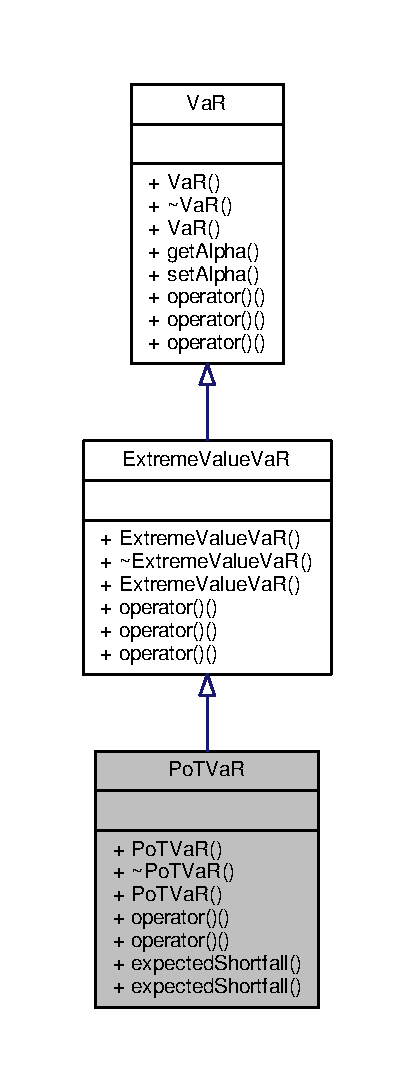
\includegraphics[width=199pt]{classPoTVaR__inherit__graph}
\end{center}
\end{figure}


Collaboration diagram for Po\+T\+VaR\+:
\nopagebreak
\begin{figure}[H]
\begin{center}
\leavevmode
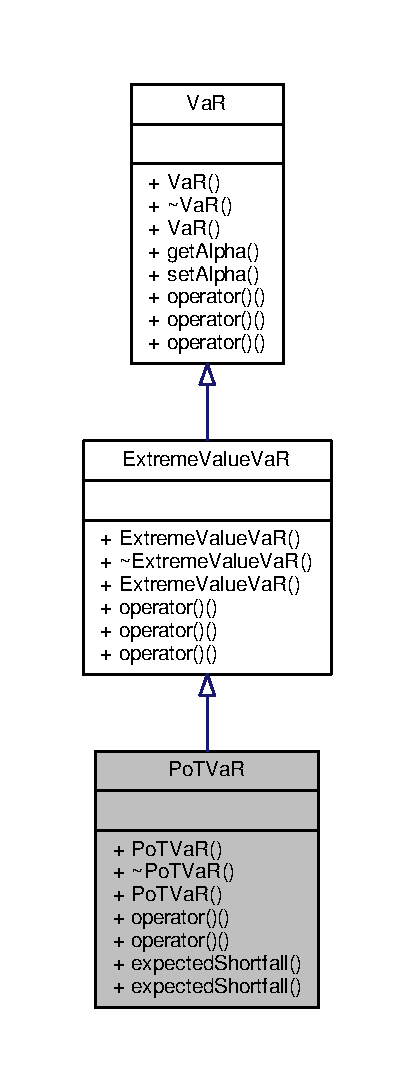
\includegraphics[width=199pt]{classPoTVaR__coll__graph}
\end{center}
\end{figure}
\subsection*{Public Member Functions}
\begin{DoxyCompactItemize}
\item 
\hyperlink{classPoTVaR_a09f126a81fbd344ba9b095a1837bbb78}{Po\+T\+VaR} (double \+\_\+u, double \+\_\+beta, double \+\_\+xi, double \+\_\+alpha=.\+05)
\item 
virtual \hyperlink{classPoTVaR_a1c80207f1679f5702f537ecea239d971}{$\sim$\+Po\+T\+VaR} ()
\item 
\hyperlink{classPoTVaR_a6a8b98090713854bd1e19fb20c2603c5}{Po\+T\+VaR} (const \hyperlink{classPoTVaR}{Po\+T\+VaR} \&other)
\item 
double \hyperlink{classPoTVaR_a7ee10c78ebe9cc0961e4344734860c97}{operator()} (const double \&ratio) const
\item 
double \hyperlink{classPoTVaR_a3360bbbeceae9bbd0c721e48586bf38c}{operator()} (const \hyperlink{compute__returns__eigen_8h_a1eb6a9306ef406d7975f3cbf2e247777}{Vec} \&returns) const
\begin{DoxyCompactList}\small\item\em Compute ratio of exceedance and \hyperlink{classVaR}{VaR}. \end{DoxyCompactList}\item 
double \hyperlink{classPoTVaR_a2a133206a1cec2c101cb68402c3c4041}{expected\+Shortfall} (const double \&ratio) const
\item 
double \hyperlink{classPoTVaR_ad89b58b1c90111b1af8568a16e8d6b96}{expected\+Shortfall} (const \hyperlink{compute__returns__eigen_8h_a1eb6a9306ef406d7975f3cbf2e247777}{Vec} \&returns) const
\begin{DoxyCompactList}\small\item\em Compute ratio of exceedance and ES. \end{DoxyCompactList}\end{DoxyCompactItemize}


\subsection{Detailed Description}
Peak over Threshold (P\+OT)

Use generalized Pareto distribution 

\subsection{Constructor \& Destructor Documentation}
\hypertarget{classPoTVaR_a09f126a81fbd344ba9b095a1837bbb78}{}\label{classPoTVaR_a09f126a81fbd344ba9b095a1837bbb78} 
\index{Po\+T\+VaR@{Po\+T\+VaR}!Po\+T\+VaR@{Po\+T\+VaR}}
\index{Po\+T\+VaR@{Po\+T\+VaR}!Po\+T\+VaR@{Po\+T\+VaR}}
\subsubsection{\texorpdfstring{Po\+T\+Va\+R()}{PoTVaR()}\hspace{0.1cm}{\footnotesize\ttfamily [1/2]}}
{\footnotesize\ttfamily Po\+T\+Va\+R\+::\+Po\+T\+VaR (\begin{DoxyParamCaption}\item[{double}]{\+\_\+u,  }\item[{double}]{\+\_\+beta,  }\item[{double}]{\+\_\+xi,  }\item[{double}]{\+\_\+alpha = {\ttfamily .05} }\end{DoxyParamCaption})}


\begin{DoxyParams}{Parameters}
{\em u} & threshold \\
\hline
{\em beta} & scale parameter \\
\hline
{\em xi} & $\xi$ should be $>$ 0 \\
\hline
\end{DoxyParams}
\hypertarget{classPoTVaR_a1c80207f1679f5702f537ecea239d971}{}\label{classPoTVaR_a1c80207f1679f5702f537ecea239d971} 
\index{Po\+T\+VaR@{Po\+T\+VaR}!````~Po\+T\+VaR@{$\sim$\+Po\+T\+VaR}}
\index{````~Po\+T\+VaR@{$\sim$\+Po\+T\+VaR}!Po\+T\+VaR@{Po\+T\+VaR}}
\subsubsection{\texorpdfstring{$\sim$\+Po\+T\+Va\+R()}{~PoTVaR()}}
{\footnotesize\ttfamily virtual Po\+T\+Va\+R\+::$\sim$\+Po\+T\+VaR (\begin{DoxyParamCaption}{ }\end{DoxyParamCaption})\hspace{0.3cm}{\ttfamily [inline]}, {\ttfamily [virtual]}}

\hypertarget{classPoTVaR_a6a8b98090713854bd1e19fb20c2603c5}{}\label{classPoTVaR_a6a8b98090713854bd1e19fb20c2603c5} 
\index{Po\+T\+VaR@{Po\+T\+VaR}!Po\+T\+VaR@{Po\+T\+VaR}}
\index{Po\+T\+VaR@{Po\+T\+VaR}!Po\+T\+VaR@{Po\+T\+VaR}}
\subsubsection{\texorpdfstring{Po\+T\+Va\+R()}{PoTVaR()}\hspace{0.1cm}{\footnotesize\ttfamily [2/2]}}
{\footnotesize\ttfamily Po\+T\+Va\+R\+::\+Po\+T\+VaR (\begin{DoxyParamCaption}\item[{const \hyperlink{classPoTVaR}{Po\+T\+VaR} \&}]{other }\end{DoxyParamCaption})}



\subsection{Member Function Documentation}
\hypertarget{classPoTVaR_a2a133206a1cec2c101cb68402c3c4041}{}\label{classPoTVaR_a2a133206a1cec2c101cb68402c3c4041} 
\index{Po\+T\+VaR@{Po\+T\+VaR}!expected\+Shortfall@{expected\+Shortfall}}
\index{expected\+Shortfall@{expected\+Shortfall}!Po\+T\+VaR@{Po\+T\+VaR}}
\subsubsection{\texorpdfstring{expected\+Shortfall()}{expectedShortfall()}\hspace{0.1cm}{\footnotesize\ttfamily [1/2]}}
{\footnotesize\ttfamily double Po\+T\+Va\+R\+::expected\+Shortfall (\begin{DoxyParamCaption}\item[{const double \&}]{ratio }\end{DoxyParamCaption}) const}

\hypertarget{classPoTVaR_ad89b58b1c90111b1af8568a16e8d6b96}{}\label{classPoTVaR_ad89b58b1c90111b1af8568a16e8d6b96} 
\index{Po\+T\+VaR@{Po\+T\+VaR}!expected\+Shortfall@{expected\+Shortfall}}
\index{expected\+Shortfall@{expected\+Shortfall}!Po\+T\+VaR@{Po\+T\+VaR}}
\subsubsection{\texorpdfstring{expected\+Shortfall()}{expectedShortfall()}\hspace{0.1cm}{\footnotesize\ttfamily [2/2]}}
{\footnotesize\ttfamily double Po\+T\+Va\+R\+::expected\+Shortfall (\begin{DoxyParamCaption}\item[{const \hyperlink{compute__returns__eigen_8h_a1eb6a9306ef406d7975f3cbf2e247777}{Vec} \&}]{returns }\end{DoxyParamCaption}) const}



Compute ratio of exceedance and ES. 

\hypertarget{classPoTVaR_a7ee10c78ebe9cc0961e4344734860c97}{}\label{classPoTVaR_a7ee10c78ebe9cc0961e4344734860c97} 
\index{Po\+T\+VaR@{Po\+T\+VaR}!operator()@{operator()}}
\index{operator()@{operator()}!Po\+T\+VaR@{Po\+T\+VaR}}
\subsubsection{\texorpdfstring{operator()()}{operator()()}\hspace{0.1cm}{\footnotesize\ttfamily [1/2]}}
{\footnotesize\ttfamily double Po\+T\+Va\+R\+::operator() (\begin{DoxyParamCaption}\item[{const double \&}]{ratio }\end{DoxyParamCaption}) const}

Compute \hyperlink{classVaR}{VaR} 
\begin{DoxyParams}{Parameters}
{\em ratio} & \# of obs in excess over threshold \\
\hline
\end{DoxyParams}
\hypertarget{classPoTVaR_a3360bbbeceae9bbd0c721e48586bf38c}{}\label{classPoTVaR_a3360bbbeceae9bbd0c721e48586bf38c} 
\index{Po\+T\+VaR@{Po\+T\+VaR}!operator()@{operator()}}
\index{operator()@{operator()}!Po\+T\+VaR@{Po\+T\+VaR}}
\subsubsection{\texorpdfstring{operator()()}{operator()()}\hspace{0.1cm}{\footnotesize\ttfamily [2/2]}}
{\footnotesize\ttfamily double Po\+T\+Va\+R\+::operator() (\begin{DoxyParamCaption}\item[{const \hyperlink{compute__returns__eigen_8h_a1eb6a9306ef406d7975f3cbf2e247777}{Vec} \&}]{returns }\end{DoxyParamCaption}) const\hspace{0.3cm}{\ttfamily [virtual]}}



Compute ratio of exceedance and \hyperlink{classVaR}{VaR}. 



Implements \hyperlink{classExtremeValueVaR_a3be021ee0faa2285bcb6be19815e3dc7}{Extreme\+Value\+VaR}.



The documentation for this class was generated from the following file\+:\begin{DoxyCompactItemize}
\item 
\hyperlink{var__model_8h}{var\+\_\+model.\+h}\end{DoxyCompactItemize}

\hypertarget{classRiskMetricsVaR}{}\section{Risk\+Metrics\+VaR Class Reference}
\label{classRiskMetricsVaR}\index{Risk\+Metrics\+VaR@{Risk\+Metrics\+VaR}}


Compute Risk metrics \hyperlink{classVaR}{VaR} aka Exponential Weight Moving Average (E\+W\+MA)  




{\ttfamily \#include $<$var\+\_\+model.\+h$>$}



Inheritance diagram for Risk\+Metrics\+VaR\+:
\nopagebreak
\begin{figure}[H]
\begin{center}
\leavevmode
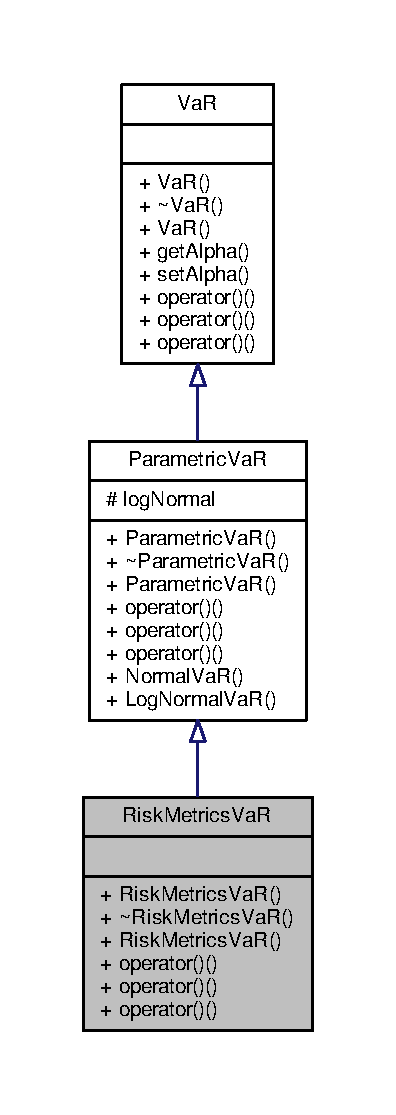
\includegraphics[width=190pt]{classRiskMetricsVaR__inherit__graph}
\end{center}
\end{figure}


Collaboration diagram for Risk\+Metrics\+VaR\+:
\nopagebreak
\begin{figure}[H]
\begin{center}
\leavevmode
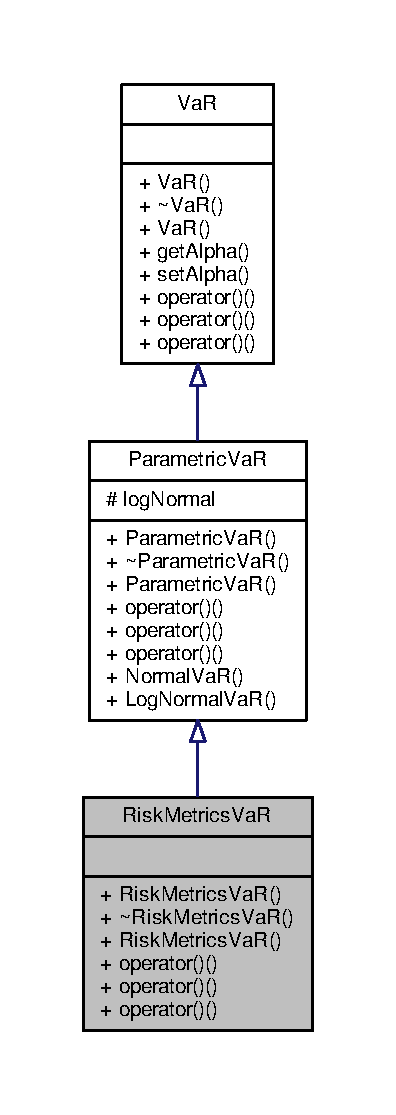
\includegraphics[width=190pt]{classRiskMetricsVaR__coll__graph}
\end{center}
\end{figure}
\subsection*{Public Member Functions}
\begin{DoxyCompactItemize}
\item 
\hyperlink{classRiskMetricsVaR_a8e7cd1fce104f7b8ea679a81dbf680c0}{Risk\+Metrics\+VaR} (double \+\_\+alpha=.\+05, double \+\_\+lambda=.\+94, bool \+\_\+log\+Normal=false)
\item 
virtual \hyperlink{classRiskMetricsVaR_a97ad6e0fe38cfef62f10da67d542bdd0}{$\sim$\+Risk\+Metrics\+VaR} ()
\item 
\hyperlink{classRiskMetricsVaR_a296438226de45455204287f234034935}{Risk\+Metrics\+VaR} (const \hyperlink{classRiskMetricsVaR}{Risk\+Metrics\+VaR} \&other)
\item 
double \hyperlink{classRiskMetricsVaR_a801fc34d2327f8fffc1315a5a9aa9df1}{operator()} (double \+\_\+mean\+Return, double \+\_\+sigmatminus1, double \+\_\+returnt) const
\item 
double \hyperlink{classRiskMetricsVaR_ab83bde7047dc8e501b8e8ea115cf5e7b}{operator()} (double \+\_\+mean\+Return, const \hyperlink{compute__returns__eigen_8h_a1eb6a9306ef406d7975f3cbf2e247777}{Vec} \&returns) const
\item 
double \hyperlink{classRiskMetricsVaR_a3e79a82675a93c7467451146131a2ec5}{operator()} (const \hyperlink{compute__returns__eigen_8h_a1eb6a9306ef406d7975f3cbf2e247777}{Vec} \&returns) const
\end{DoxyCompactItemize}
\subsection*{Additional Inherited Members}


\subsection{Detailed Description}
Compute Risk metrics \hyperlink{classVaR}{VaR} aka Exponential Weight Moving Average (E\+W\+MA) 

\subsection{Constructor \& Destructor Documentation}
\hypertarget{classRiskMetricsVaR_a8e7cd1fce104f7b8ea679a81dbf680c0}{}\label{classRiskMetricsVaR_a8e7cd1fce104f7b8ea679a81dbf680c0} 
\index{Risk\+Metrics\+VaR@{Risk\+Metrics\+VaR}!Risk\+Metrics\+VaR@{Risk\+Metrics\+VaR}}
\index{Risk\+Metrics\+VaR@{Risk\+Metrics\+VaR}!Risk\+Metrics\+VaR@{Risk\+Metrics\+VaR}}
\subsubsection{\texorpdfstring{Risk\+Metrics\+Va\+R()}{RiskMetricsVaR()}\hspace{0.1cm}{\footnotesize\ttfamily [1/2]}}
{\footnotesize\ttfamily Risk\+Metrics\+Va\+R\+::\+Risk\+Metrics\+VaR (\begin{DoxyParamCaption}\item[{double}]{\+\_\+alpha = {\ttfamily .05},  }\item[{double}]{\+\_\+lambda = {\ttfamily .94},  }\item[{bool}]{\+\_\+log\+Normal = {\ttfamily false} }\end{DoxyParamCaption})}

\hypertarget{classRiskMetricsVaR_a97ad6e0fe38cfef62f10da67d542bdd0}{}\label{classRiskMetricsVaR_a97ad6e0fe38cfef62f10da67d542bdd0} 
\index{Risk\+Metrics\+VaR@{Risk\+Metrics\+VaR}!````~Risk\+Metrics\+VaR@{$\sim$\+Risk\+Metrics\+VaR}}
\index{````~Risk\+Metrics\+VaR@{$\sim$\+Risk\+Metrics\+VaR}!Risk\+Metrics\+VaR@{Risk\+Metrics\+VaR}}
\subsubsection{\texorpdfstring{$\sim$\+Risk\+Metrics\+Va\+R()}{~RiskMetricsVaR()}}
{\footnotesize\ttfamily virtual Risk\+Metrics\+Va\+R\+::$\sim$\+Risk\+Metrics\+VaR (\begin{DoxyParamCaption}{ }\end{DoxyParamCaption})\hspace{0.3cm}{\ttfamily [inline]}, {\ttfamily [virtual]}}

\hypertarget{classRiskMetricsVaR_a296438226de45455204287f234034935}{}\label{classRiskMetricsVaR_a296438226de45455204287f234034935} 
\index{Risk\+Metrics\+VaR@{Risk\+Metrics\+VaR}!Risk\+Metrics\+VaR@{Risk\+Metrics\+VaR}}
\index{Risk\+Metrics\+VaR@{Risk\+Metrics\+VaR}!Risk\+Metrics\+VaR@{Risk\+Metrics\+VaR}}
\subsubsection{\texorpdfstring{Risk\+Metrics\+Va\+R()}{RiskMetricsVaR()}\hspace{0.1cm}{\footnotesize\ttfamily [2/2]}}
{\footnotesize\ttfamily Risk\+Metrics\+Va\+R\+::\+Risk\+Metrics\+VaR (\begin{DoxyParamCaption}\item[{const \hyperlink{classRiskMetricsVaR}{Risk\+Metrics\+VaR} \&}]{other }\end{DoxyParamCaption})}



\subsection{Member Function Documentation}
\hypertarget{classRiskMetricsVaR_a801fc34d2327f8fffc1315a5a9aa9df1}{}\label{classRiskMetricsVaR_a801fc34d2327f8fffc1315a5a9aa9df1} 
\index{Risk\+Metrics\+VaR@{Risk\+Metrics\+VaR}!operator()@{operator()}}
\index{operator()@{operator()}!Risk\+Metrics\+VaR@{Risk\+Metrics\+VaR}}
\subsubsection{\texorpdfstring{operator()()}{operator()()}\hspace{0.1cm}{\footnotesize\ttfamily [1/3]}}
{\footnotesize\ttfamily double Risk\+Metrics\+Va\+R\+::operator() (\begin{DoxyParamCaption}\item[{double}]{\+\_\+mean\+Return,  }\item[{double}]{\+\_\+sigmatminus1,  }\item[{double}]{\+\_\+returnt }\end{DoxyParamCaption}) const\hspace{0.3cm}{\ttfamily [virtual]}}



Implements \hyperlink{classParametricVaR_a54589e13bb45da786d574656eb67b5fb}{Parametric\+VaR}.

\hypertarget{classRiskMetricsVaR_ab83bde7047dc8e501b8e8ea115cf5e7b}{}\label{classRiskMetricsVaR_ab83bde7047dc8e501b8e8ea115cf5e7b} 
\index{Risk\+Metrics\+VaR@{Risk\+Metrics\+VaR}!operator()@{operator()}}
\index{operator()@{operator()}!Risk\+Metrics\+VaR@{Risk\+Metrics\+VaR}}
\subsubsection{\texorpdfstring{operator()()}{operator()()}\hspace{0.1cm}{\footnotesize\ttfamily [2/3]}}
{\footnotesize\ttfamily double Risk\+Metrics\+Va\+R\+::operator() (\begin{DoxyParamCaption}\item[{double}]{\+\_\+mean\+Return,  }\item[{const \hyperlink{compute__returns__eigen_8h_a1eb6a9306ef406d7975f3cbf2e247777}{Vec} \&}]{returns }\end{DoxyParamCaption}) const\hspace{0.3cm}{\ttfamily [virtual]}}



Implements \hyperlink{classParametricVaR_a5fda9d0e1033ff6e93dd112555ee5e0b}{Parametric\+VaR}.

\hypertarget{classRiskMetricsVaR_a3e79a82675a93c7467451146131a2ec5}{}\label{classRiskMetricsVaR_a3e79a82675a93c7467451146131a2ec5} 
\index{Risk\+Metrics\+VaR@{Risk\+Metrics\+VaR}!operator()@{operator()}}
\index{operator()@{operator()}!Risk\+Metrics\+VaR@{Risk\+Metrics\+VaR}}
\subsubsection{\texorpdfstring{operator()()}{operator()()}\hspace{0.1cm}{\footnotesize\ttfamily [3/3]}}
{\footnotesize\ttfamily double Risk\+Metrics\+Va\+R\+::operator() (\begin{DoxyParamCaption}\item[{const \hyperlink{compute__returns__eigen_8h_a1eb6a9306ef406d7975f3cbf2e247777}{Vec} \&}]{returns }\end{DoxyParamCaption}) const\hspace{0.3cm}{\ttfamily [virtual]}}



Implements \hyperlink{classParametricVaR_aa07f1d64aff5abf484835cd9105af9c9}{Parametric\+VaR}.



The documentation for this class was generated from the following file\+:\begin{DoxyCompactItemize}
\item 
\hyperlink{var__model_8h}{var\+\_\+model.\+h}\end{DoxyCompactItemize}

\hypertarget{classrng}{}\section{rng Class Reference}
\label{classrng}\index{rng@{rng}}


Mersenne-\/\+Twister pseudo random number generator.  




{\ttfamily \#include $<$rng.\+h$>$}



Collaboration diagram for rng\+:
\nopagebreak
\begin{figure}[H]
\begin{center}
\leavevmode
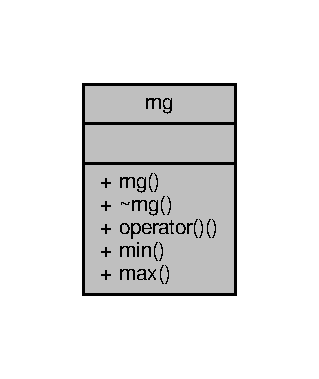
\includegraphics[width=153pt]{classrng__coll__graph}
\end{center}
\end{figure}
\subsection*{Public Member Functions}
\begin{DoxyCompactItemize}
\item 
\hyperlink{classrng_a42a6b92cac3b2a289f8d21fe8cfe6101}{rng} ()
\item 
\hyperlink{classrng_a6fca2df7036b5f2f76b9b642523f5d19}{$\sim$rng} ()
\item 
double \hyperlink{classrng_a58c53a0d8e075b75c4d1eb4d4af5fe7f}{operator()} ()
\begin{DoxyCompactList}\small\item\em Go to next number in pseudo-\/sequence. \end{DoxyCompactList}\item 
uint32\+\_\+t \hyperlink{classrng_a2619e124008ebc19fef93983f50eaf50}{min} ()
\item 
uint32\+\_\+t \hyperlink{classrng_aea990d0e1df0fc4a5850d7a3dedee633}{max} ()
\end{DoxyCompactItemize}


\subsection{Detailed Description}
Mersenne-\/\+Twister pseudo random number generator. 

\subsection{Constructor \& Destructor Documentation}
\hypertarget{classrng_a42a6b92cac3b2a289f8d21fe8cfe6101}{}\label{classrng_a42a6b92cac3b2a289f8d21fe8cfe6101} 
\index{rng@{rng}!rng@{rng}}
\index{rng@{rng}!rng@{rng}}
\subsubsection{\texorpdfstring{rng()}{rng()}}
{\footnotesize\ttfamily rng\+::rng (\begin{DoxyParamCaption}{ }\end{DoxyParamCaption})\hspace{0.3cm}{\ttfamily [inline]}}

\hypertarget{classrng_a6fca2df7036b5f2f76b9b642523f5d19}{}\label{classrng_a6fca2df7036b5f2f76b9b642523f5d19} 
\index{rng@{rng}!````~rng@{$\sim$rng}}
\index{````~rng@{$\sim$rng}!rng@{rng}}
\subsubsection{\texorpdfstring{$\sim$rng()}{~rng()}}
{\footnotesize\ttfamily rng\+::$\sim$rng (\begin{DoxyParamCaption}{ }\end{DoxyParamCaption})\hspace{0.3cm}{\ttfamily [inline]}}



\subsection{Member Function Documentation}
\hypertarget{classrng_aea990d0e1df0fc4a5850d7a3dedee633}{}\label{classrng_aea990d0e1df0fc4a5850d7a3dedee633} 
\index{rng@{rng}!max@{max}}
\index{max@{max}!rng@{rng}}
\subsubsection{\texorpdfstring{max()}{max()}}
{\footnotesize\ttfamily uint32\+\_\+t rng\+::max (\begin{DoxyParamCaption}{ }\end{DoxyParamCaption})\hspace{0.3cm}{\ttfamily [inline]}}

\hypertarget{classrng_a2619e124008ebc19fef93983f50eaf50}{}\label{classrng_a2619e124008ebc19fef93983f50eaf50} 
\index{rng@{rng}!min@{min}}
\index{min@{min}!rng@{rng}}
\subsubsection{\texorpdfstring{min()}{min()}}
{\footnotesize\ttfamily uint32\+\_\+t rng\+::min (\begin{DoxyParamCaption}{ }\end{DoxyParamCaption})\hspace{0.3cm}{\ttfamily [inline]}}

\hypertarget{classrng_a58c53a0d8e075b75c4d1eb4d4af5fe7f}{}\label{classrng_a58c53a0d8e075b75c4d1eb4d4af5fe7f} 
\index{rng@{rng}!operator()@{operator()}}
\index{operator()@{operator()}!rng@{rng}}
\subsubsection{\texorpdfstring{operator()()}{operator()()}}
{\footnotesize\ttfamily double rng\+::operator() (\begin{DoxyParamCaption}{ }\end{DoxyParamCaption})\hspace{0.3cm}{\ttfamily [inline]}}



Go to next number in pseudo-\/sequence. 



The documentation for this class was generated from the following file\+:\begin{DoxyCompactItemize}
\item 
\hyperlink{rng_8h}{rng.\+h}\end{DoxyCompactItemize}

\hypertarget{classVaR}{}\section{VaR Class Reference}
\label{classVaR}\index{VaR@{VaR}}


{\ttfamily \#include $<$var\+\_\+model.\+h$>$}



Inheritance diagram for VaR\+:
\nopagebreak
\begin{figure}[H]
\begin{center}
\leavevmode
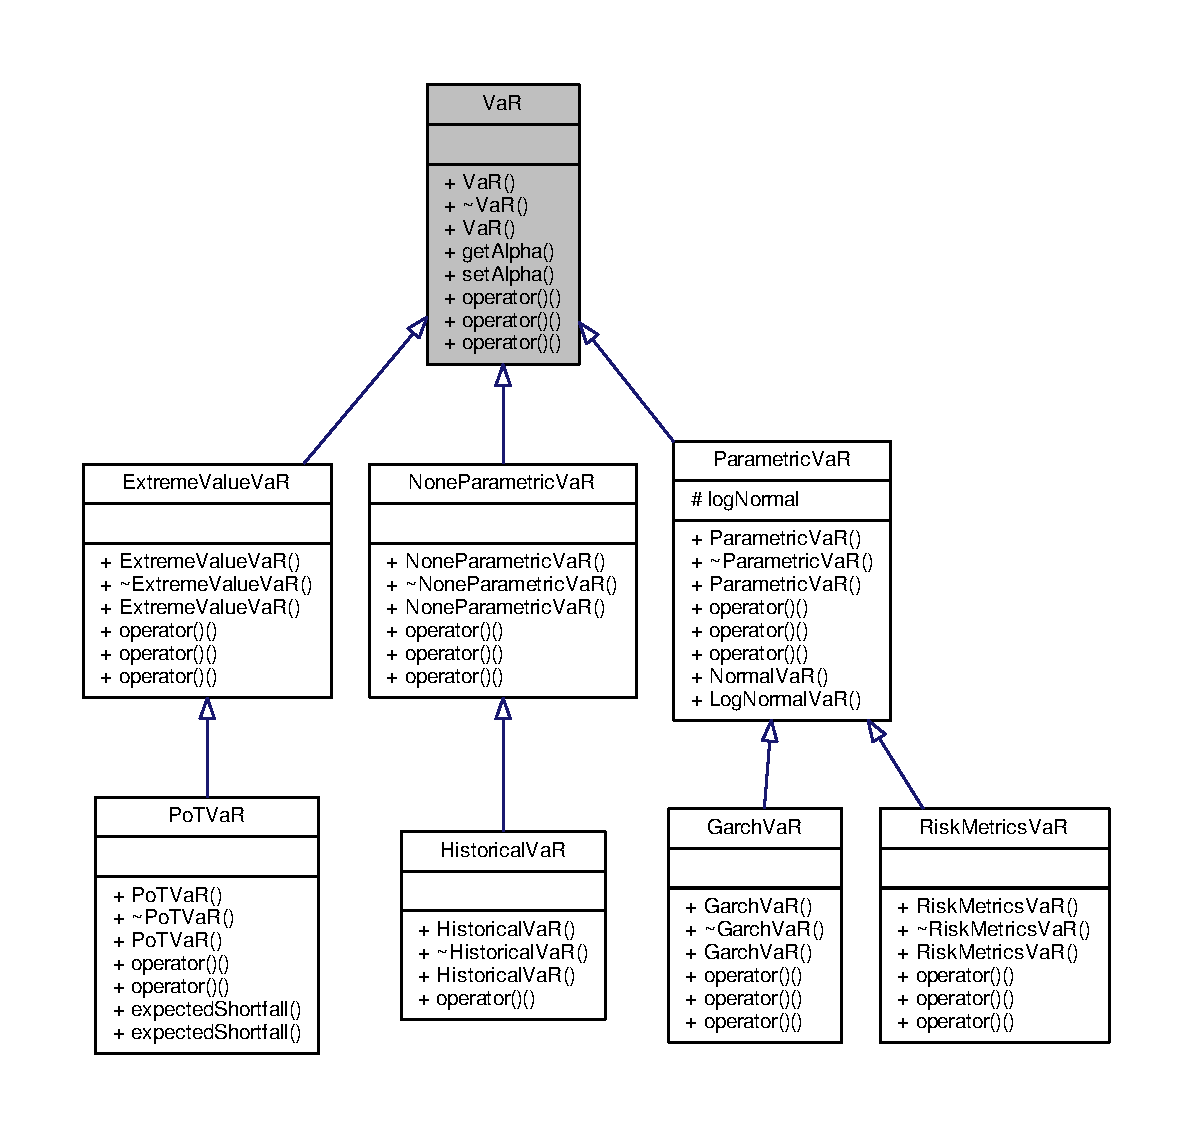
\includegraphics[width=350pt]{classVaR__inherit__graph}
\end{center}
\end{figure}


Collaboration diagram for VaR\+:
\nopagebreak
\begin{figure}[H]
\begin{center}
\leavevmode
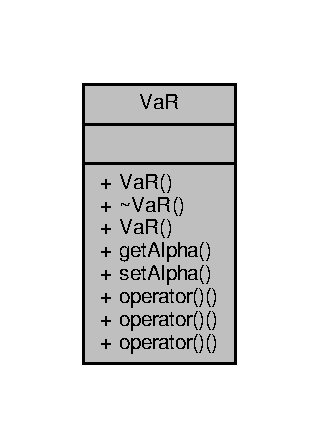
\includegraphics[width=153pt]{classVaR__coll__graph}
\end{center}
\end{figure}
\subsection*{Public Member Functions}
\begin{DoxyCompactItemize}
\item 
\hyperlink{classVaR_a7ee643c7cd27654b357d80718a830750}{VaR} (double \+\_\+alpha=.\+05)
\item 
virtual \hyperlink{classVaR_af1492f7ffa13239a77af0a2c647f8358}{$\sim$\+VaR} ()
\item 
\hyperlink{classVaR_a21cafaf403766ed1f5ba3d957357d789}{VaR} (const \hyperlink{classVaR}{VaR} \&other)
\item 
double \hyperlink{classVaR_aa2c6adc33bdf14b0908f4586254726c9}{get\+Alpha} () const
\item 
void \hyperlink{classVaR_a5834560649dcbe686a47eaba4f0359b9}{set\+Alpha} (double \+\_\+alpha)
\item 
virtual double \hyperlink{classVaR_a28e1a1be9e386ed4e8503e54db4033bd}{operator()} (double \+\_\+mean\+Return, double \+\_\+sigmatminus1, double \+\_\+returnt) const =0
\item 
virtual double \hyperlink{classVaR_a31cb62626488715a9133679feaba31e5}{operator()} (double \+\_\+mean\+Return, const \hyperlink{compute__returns__eigen_8h_a1eb6a9306ef406d7975f3cbf2e247777}{Vec} \&returns) const =0
\item 
virtual double \hyperlink{classVaR_a1bd868d9953bfaeb49f5bf7d16986631}{operator()} (const \hyperlink{compute__returns__eigen_8h_a1eb6a9306ef406d7975f3cbf2e247777}{Vec} \&returns) const =0
\end{DoxyCompactItemize}


\subsection{Detailed Description}
Abstract base class

Define different Value at Risk (\hyperlink{classVaR}{VaR}) models 

\subsection{Constructor \& Destructor Documentation}
\hypertarget{classVaR_a7ee643c7cd27654b357d80718a830750}{}\label{classVaR_a7ee643c7cd27654b357d80718a830750} 
\index{VaR@{VaR}!VaR@{VaR}}
\index{VaR@{VaR}!VaR@{VaR}}
\subsubsection{\texorpdfstring{Va\+R()}{VaR()}\hspace{0.1cm}{\footnotesize\ttfamily [1/2]}}
{\footnotesize\ttfamily Va\+R\+::\+VaR (\begin{DoxyParamCaption}\item[{double}]{\+\_\+alpha = {\ttfamily .05} }\end{DoxyParamCaption})}

\hypertarget{classVaR_af1492f7ffa13239a77af0a2c647f8358}{}\label{classVaR_af1492f7ffa13239a77af0a2c647f8358} 
\index{VaR@{VaR}!````~VaR@{$\sim$\+VaR}}
\index{````~VaR@{$\sim$\+VaR}!VaR@{VaR}}
\subsubsection{\texorpdfstring{$\sim$\+Va\+R()}{~VaR()}}
{\footnotesize\ttfamily virtual Va\+R\+::$\sim$\+VaR (\begin{DoxyParamCaption}{ }\end{DoxyParamCaption})\hspace{0.3cm}{\ttfamily [inline]}, {\ttfamily [virtual]}}

\hypertarget{classVaR_a21cafaf403766ed1f5ba3d957357d789}{}\label{classVaR_a21cafaf403766ed1f5ba3d957357d789} 
\index{VaR@{VaR}!VaR@{VaR}}
\index{VaR@{VaR}!VaR@{VaR}}
\subsubsection{\texorpdfstring{Va\+R()}{VaR()}\hspace{0.1cm}{\footnotesize\ttfamily [2/2]}}
{\footnotesize\ttfamily Va\+R\+::\+VaR (\begin{DoxyParamCaption}\item[{const \hyperlink{classVaR}{VaR} \&}]{other }\end{DoxyParamCaption})}



\subsection{Member Function Documentation}
\hypertarget{classVaR_aa2c6adc33bdf14b0908f4586254726c9}{}\label{classVaR_aa2c6adc33bdf14b0908f4586254726c9} 
\index{VaR@{VaR}!get\+Alpha@{get\+Alpha}}
\index{get\+Alpha@{get\+Alpha}!VaR@{VaR}}
\subsubsection{\texorpdfstring{get\+Alpha()}{getAlpha()}}
{\footnotesize\ttfamily double Va\+R\+::get\+Alpha (\begin{DoxyParamCaption}{ }\end{DoxyParamCaption}) const}

\hypertarget{classVaR_a28e1a1be9e386ed4e8503e54db4033bd}{}\label{classVaR_a28e1a1be9e386ed4e8503e54db4033bd} 
\index{VaR@{VaR}!operator()@{operator()}}
\index{operator()@{operator()}!VaR@{VaR}}
\subsubsection{\texorpdfstring{operator()()}{operator()()}\hspace{0.1cm}{\footnotesize\ttfamily [1/3]}}
{\footnotesize\ttfamily virtual double Va\+R\+::operator() (\begin{DoxyParamCaption}\item[{double}]{\+\_\+mean\+Return,  }\item[{double}]{\+\_\+sigmatminus1,  }\item[{double}]{\+\_\+returnt }\end{DoxyParamCaption}) const\hspace{0.3cm}{\ttfamily [pure virtual]}}



Implemented in \hyperlink{classExtremeValueVaR_ad6d31417001a3ee1b75592806d21ae8b}{Extreme\+Value\+VaR}, \hyperlink{classNoneParametricVaR_ab22e4237802535880a932097aeaf003b}{None\+Parametric\+VaR}, \hyperlink{classGarchVaR_a6aec8c89e48d2b2f356669ed3300f456}{Garch\+VaR}, \hyperlink{classRiskMetricsVaR_a801fc34d2327f8fffc1315a5a9aa9df1}{Risk\+Metrics\+VaR}, and \hyperlink{classParametricVaR_a54589e13bb45da786d574656eb67b5fb}{Parametric\+VaR}.

\hypertarget{classVaR_a31cb62626488715a9133679feaba31e5}{}\label{classVaR_a31cb62626488715a9133679feaba31e5} 
\index{VaR@{VaR}!operator()@{operator()}}
\index{operator()@{operator()}!VaR@{VaR}}
\subsubsection{\texorpdfstring{operator()()}{operator()()}\hspace{0.1cm}{\footnotesize\ttfamily [2/3]}}
{\footnotesize\ttfamily virtual double Va\+R\+::operator() (\begin{DoxyParamCaption}\item[{double}]{\+\_\+mean\+Return,  }\item[{const \hyperlink{compute__returns__eigen_8h_a1eb6a9306ef406d7975f3cbf2e247777}{Vec} \&}]{returns }\end{DoxyParamCaption}) const\hspace{0.3cm}{\ttfamily [pure virtual]}}



Implemented in \hyperlink{classExtremeValueVaR_a8dfe4d515f7e4d0260b3ac87c1a52b5f}{Extreme\+Value\+VaR}, \hyperlink{classHistoricalVaR_a472b04dc9a4c5989be0e7198bc9c4189}{Historical\+VaR}, \hyperlink{classNoneParametricVaR_a958aae1b9bc03a8ef87295df30db76f7}{None\+Parametric\+VaR}, \hyperlink{classGarchVaR_ab7e9583566b26a64017edbbfb63f3e89}{Garch\+VaR}, \hyperlink{classRiskMetricsVaR_ab83bde7047dc8e501b8e8ea115cf5e7b}{Risk\+Metrics\+VaR}, and \hyperlink{classParametricVaR_a5fda9d0e1033ff6e93dd112555ee5e0b}{Parametric\+VaR}.

\hypertarget{classVaR_a1bd868d9953bfaeb49f5bf7d16986631}{}\label{classVaR_a1bd868d9953bfaeb49f5bf7d16986631} 
\index{VaR@{VaR}!operator()@{operator()}}
\index{operator()@{operator()}!VaR@{VaR}}
\subsubsection{\texorpdfstring{operator()()}{operator()()}\hspace{0.1cm}{\footnotesize\ttfamily [3/3]}}
{\footnotesize\ttfamily virtual double Va\+R\+::operator() (\begin{DoxyParamCaption}\item[{const \hyperlink{compute__returns__eigen_8h_a1eb6a9306ef406d7975f3cbf2e247777}{Vec} \&}]{returns }\end{DoxyParamCaption}) const\hspace{0.3cm}{\ttfamily [pure virtual]}}



Implemented in \hyperlink{classPoTVaR_a3360bbbeceae9bbd0c721e48586bf38c}{Po\+T\+VaR}, \hyperlink{classExtremeValueVaR_a3be021ee0faa2285bcb6be19815e3dc7}{Extreme\+Value\+VaR}, \hyperlink{classNoneParametricVaR_a181d6152dcbdc7ce323e5d4b672a14f8}{None\+Parametric\+VaR}, \hyperlink{classGarchVaR_ac6d01b6567a6d0629cd95be716677763}{Garch\+VaR}, \hyperlink{classRiskMetricsVaR_a3e79a82675a93c7467451146131a2ec5}{Risk\+Metrics\+VaR}, and \hyperlink{classParametricVaR_aa07f1d64aff5abf484835cd9105af9c9}{Parametric\+VaR}.

\hypertarget{classVaR_a5834560649dcbe686a47eaba4f0359b9}{}\label{classVaR_a5834560649dcbe686a47eaba4f0359b9} 
\index{VaR@{VaR}!set\+Alpha@{set\+Alpha}}
\index{set\+Alpha@{set\+Alpha}!VaR@{VaR}}
\subsubsection{\texorpdfstring{set\+Alpha()}{setAlpha()}}
{\footnotesize\ttfamily void Va\+R\+::set\+Alpha (\begin{DoxyParamCaption}\item[{double}]{\+\_\+alpha }\end{DoxyParamCaption})}



The documentation for this class was generated from the following file\+:\begin{DoxyCompactItemize}
\item 
\hyperlink{var__model_8h}{var\+\_\+model.\+h}\end{DoxyCompactItemize}

\hypertarget{classVaRBridge}{}\section{Va\+R\+Bridge Class Reference}
\label{classVaRBridge}\index{Va\+R\+Bridge@{Va\+R\+Bridge}}


{\ttfamily \#include $<$var\+\_\+bridge.\+h$>$}



Collaboration diagram for Va\+R\+Bridge\+:
\nopagebreak
\begin{figure}[H]
\begin{center}
\leavevmode
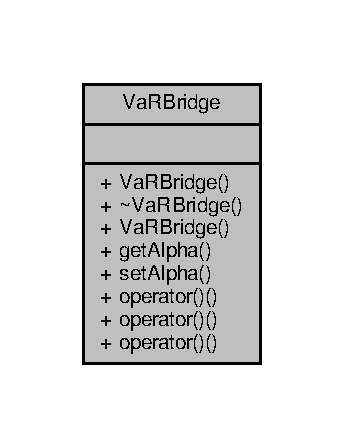
\includegraphics[width=165pt]{classVaRBridge__coll__graph}
\end{center}
\end{figure}
\subsection*{Public Member Functions}
\begin{DoxyCompactItemize}
\item 
\hyperlink{classVaRBridge_ae2a2b2437f30f28b3722a4634cc80161}{Va\+R\+Bridge} ()
\item 
\hyperlink{classVaRBridge_a876183182e5eb13a652627c69613963a}{$\sim$\+Va\+R\+Bridge} ()
\item 
\hyperlink{classVaRBridge_a2f83dff0248e044a116b4b063ca78b83}{Va\+R\+Bridge} (const \hyperlink{classVaRBridge}{Va\+R\+Bridge} \&other)=default
\item 
double \hyperlink{classVaRBridge_ab7bea293648bfa62762a3c61f162107e}{get\+Alpha} () const
\item 
void \hyperlink{classVaRBridge_a0101d9c9ee840f8720342f3639cd58dc}{set\+Alpha} (double \+\_\+alpha)
\item 
double \hyperlink{classVaRBridge_a64a2c30c69d03b4f75beb3087d3f1ea2}{operator()} (double \+\_\+mean\+Return, const \hyperlink{compute__returns__eigen_8h_a1eb6a9306ef406d7975f3cbf2e247777}{Vec} \&returns) const
\item 
double \hyperlink{classVaRBridge_ade75c664cc693524898fee6d66ae36b0}{operator()} (double \+\_\+mean\+Return, double \+\_\+sigmatminus1, double \+\_\+returnt) const
\item 
double \hyperlink{classVaRBridge_a4096da6ab396d3a92fc3423d08328bb0}{operator()} (const \hyperlink{compute__returns__eigen_8h_a1eb6a9306ef406d7975f3cbf2e247777}{Vec} \&returns) const
\end{DoxyCompactItemize}


\subsection{Constructor \& Destructor Documentation}
\hypertarget{classVaRBridge_ae2a2b2437f30f28b3722a4634cc80161}{}\label{classVaRBridge_ae2a2b2437f30f28b3722a4634cc80161} 
\index{Va\+R\+Bridge@{Va\+R\+Bridge}!Va\+R\+Bridge@{Va\+R\+Bridge}}
\index{Va\+R\+Bridge@{Va\+R\+Bridge}!Va\+R\+Bridge@{Va\+R\+Bridge}}
\subsubsection{\texorpdfstring{Va\+R\+Bridge()}{VaRBridge()}\hspace{0.1cm}{\footnotesize\ttfamily [1/2]}}
{\footnotesize\ttfamily Va\+R\+Bridge\+::\+Va\+R\+Bridge (\begin{DoxyParamCaption}{ }\end{DoxyParamCaption})}

\hypertarget{classVaRBridge_a876183182e5eb13a652627c69613963a}{}\label{classVaRBridge_a876183182e5eb13a652627c69613963a} 
\index{Va\+R\+Bridge@{Va\+R\+Bridge}!````~Va\+R\+Bridge@{$\sim$\+Va\+R\+Bridge}}
\index{````~Va\+R\+Bridge@{$\sim$\+Va\+R\+Bridge}!Va\+R\+Bridge@{Va\+R\+Bridge}}
\subsubsection{\texorpdfstring{$\sim$\+Va\+R\+Bridge()}{~VaRBridge()}}
{\footnotesize\ttfamily Va\+R\+Bridge\+::$\sim$\+Va\+R\+Bridge (\begin{DoxyParamCaption}{ }\end{DoxyParamCaption})\hspace{0.3cm}{\ttfamily [inline]}}

\hypertarget{classVaRBridge_a2f83dff0248e044a116b4b063ca78b83}{}\label{classVaRBridge_a2f83dff0248e044a116b4b063ca78b83} 
\index{Va\+R\+Bridge@{Va\+R\+Bridge}!Va\+R\+Bridge@{Va\+R\+Bridge}}
\index{Va\+R\+Bridge@{Va\+R\+Bridge}!Va\+R\+Bridge@{Va\+R\+Bridge}}
\subsubsection{\texorpdfstring{Va\+R\+Bridge()}{VaRBridge()}\hspace{0.1cm}{\footnotesize\ttfamily [2/2]}}
{\footnotesize\ttfamily Va\+R\+Bridge\+::\+Va\+R\+Bridge (\begin{DoxyParamCaption}\item[{const \hyperlink{classVaRBridge}{Va\+R\+Bridge} \&}]{other }\end{DoxyParamCaption})\hspace{0.3cm}{\ttfamily [default]}}



\subsection{Member Function Documentation}
\hypertarget{classVaRBridge_ab7bea293648bfa62762a3c61f162107e}{}\label{classVaRBridge_ab7bea293648bfa62762a3c61f162107e} 
\index{Va\+R\+Bridge@{Va\+R\+Bridge}!get\+Alpha@{get\+Alpha}}
\index{get\+Alpha@{get\+Alpha}!Va\+R\+Bridge@{Va\+R\+Bridge}}
\subsubsection{\texorpdfstring{get\+Alpha()}{getAlpha()}}
{\footnotesize\ttfamily double Va\+R\+Bridge\+::get\+Alpha (\begin{DoxyParamCaption}{ }\end{DoxyParamCaption}) const\hspace{0.3cm}{\ttfamily [inline]}}

\hypertarget{classVaRBridge_a64a2c30c69d03b4f75beb3087d3f1ea2}{}\label{classVaRBridge_a64a2c30c69d03b4f75beb3087d3f1ea2} 
\index{Va\+R\+Bridge@{Va\+R\+Bridge}!operator()@{operator()}}
\index{operator()@{operator()}!Va\+R\+Bridge@{Va\+R\+Bridge}}
\subsubsection{\texorpdfstring{operator()()}{operator()()}\hspace{0.1cm}{\footnotesize\ttfamily [1/3]}}
{\footnotesize\ttfamily double Va\+R\+Bridge\+::operator() (\begin{DoxyParamCaption}\item[{double}]{\+\_\+mean\+Return,  }\item[{const \hyperlink{compute__returns__eigen_8h_a1eb6a9306ef406d7975f3cbf2e247777}{Vec} \&}]{returns }\end{DoxyParamCaption}) const\hspace{0.3cm}{\ttfamily [inline]}}

\hypertarget{classVaRBridge_ade75c664cc693524898fee6d66ae36b0}{}\label{classVaRBridge_ade75c664cc693524898fee6d66ae36b0} 
\index{Va\+R\+Bridge@{Va\+R\+Bridge}!operator()@{operator()}}
\index{operator()@{operator()}!Va\+R\+Bridge@{Va\+R\+Bridge}}
\subsubsection{\texorpdfstring{operator()()}{operator()()}\hspace{0.1cm}{\footnotesize\ttfamily [2/3]}}
{\footnotesize\ttfamily double Va\+R\+Bridge\+::operator() (\begin{DoxyParamCaption}\item[{double}]{\+\_\+mean\+Return,  }\item[{double}]{\+\_\+sigmatminus1,  }\item[{double}]{\+\_\+returnt }\end{DoxyParamCaption}) const\hspace{0.3cm}{\ttfamily [inline]}}

\hypertarget{classVaRBridge_a4096da6ab396d3a92fc3423d08328bb0}{}\label{classVaRBridge_a4096da6ab396d3a92fc3423d08328bb0} 
\index{Va\+R\+Bridge@{Va\+R\+Bridge}!operator()@{operator()}}
\index{operator()@{operator()}!Va\+R\+Bridge@{Va\+R\+Bridge}}
\subsubsection{\texorpdfstring{operator()()}{operator()()}\hspace{0.1cm}{\footnotesize\ttfamily [3/3]}}
{\footnotesize\ttfamily double Va\+R\+Bridge\+::operator() (\begin{DoxyParamCaption}\item[{const \hyperlink{compute__returns__eigen_8h_a1eb6a9306ef406d7975f3cbf2e247777}{Vec} \&}]{returns }\end{DoxyParamCaption}) const\hspace{0.3cm}{\ttfamily [inline]}}

\hypertarget{classVaRBridge_a0101d9c9ee840f8720342f3639cd58dc}{}\label{classVaRBridge_a0101d9c9ee840f8720342f3639cd58dc} 
\index{Va\+R\+Bridge@{Va\+R\+Bridge}!set\+Alpha@{set\+Alpha}}
\index{set\+Alpha@{set\+Alpha}!Va\+R\+Bridge@{Va\+R\+Bridge}}
\subsubsection{\texorpdfstring{set\+Alpha()}{setAlpha()}}
{\footnotesize\ttfamily void Va\+R\+Bridge\+::set\+Alpha (\begin{DoxyParamCaption}\item[{double}]{\+\_\+alpha }\end{DoxyParamCaption})\hspace{0.3cm}{\ttfamily [inline]}}



The documentation for this class was generated from the following file\+:\begin{DoxyCompactItemize}
\item 
\hyperlink{var__bridge_8h}{var\+\_\+bridge.\+h}\end{DoxyCompactItemize}

\hypertarget{classVaRCompute}{}\section{Va\+R\+Compute$<$ T, U $>$ Class Template Reference}
\label{classVaRCompute}\index{Va\+R\+Compute$<$ T, U $>$@{Va\+R\+Compute$<$ T, U $>$}}


Compute \hyperlink{classVaR}{VaR}.  




{\ttfamily \#include $<$compute\+\_\+var.\+h$>$}



Inheritance diagram for Va\+R\+Compute$<$ T, U $>$\+:
\nopagebreak
\begin{figure}[H]
\begin{center}
\leavevmode
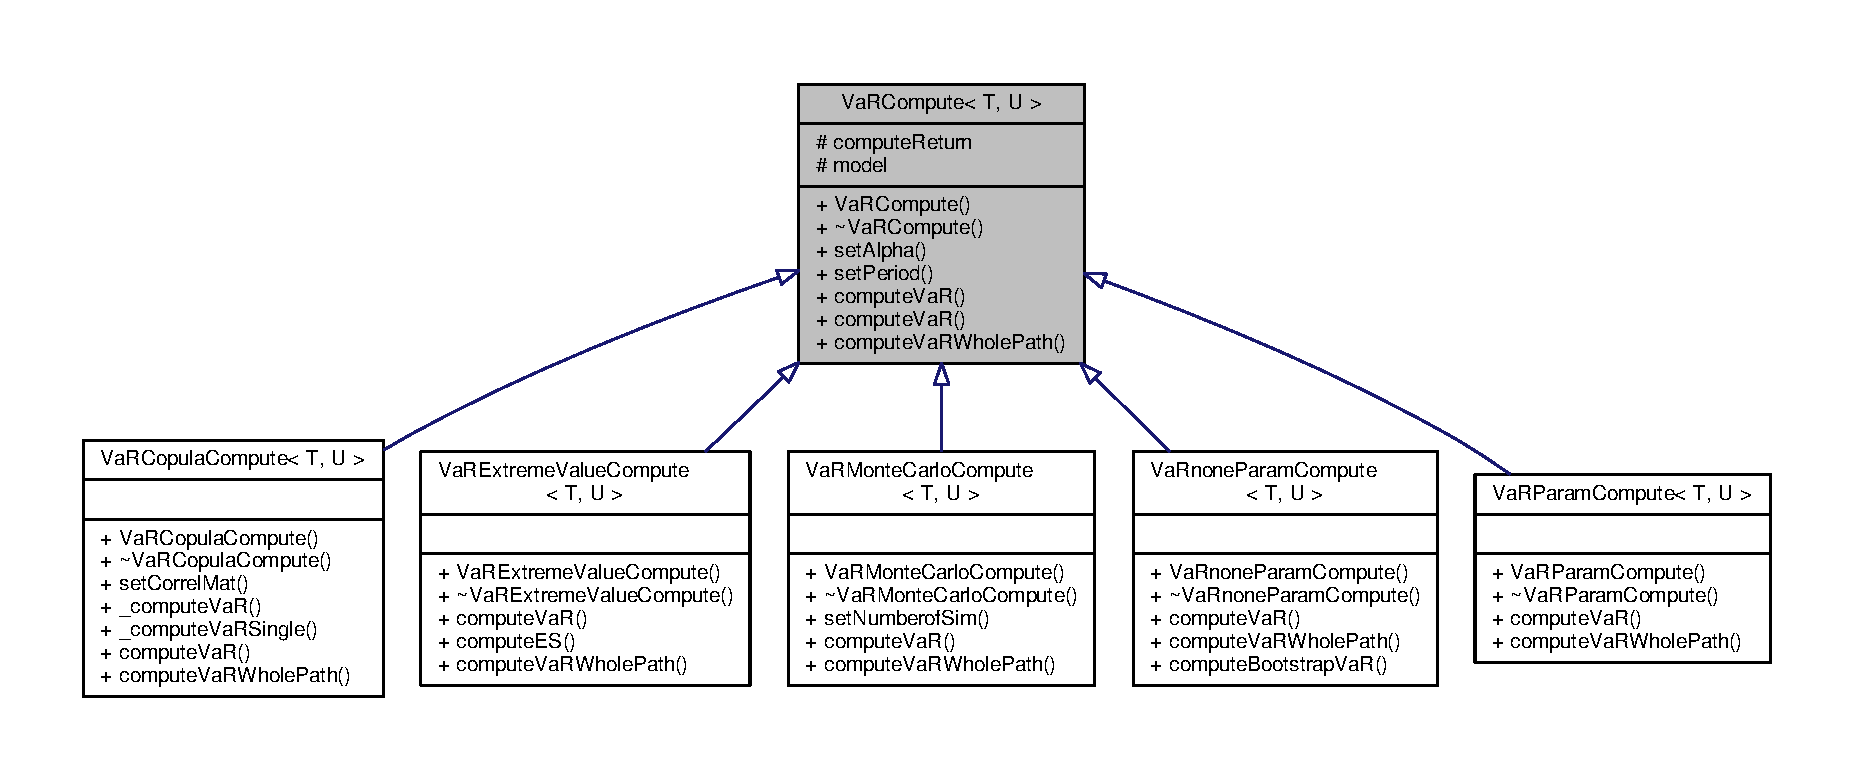
\includegraphics[width=350pt]{classVaRCompute__inherit__graph}
\end{center}
\end{figure}


Collaboration diagram for Va\+R\+Compute$<$ T, U $>$\+:
\nopagebreak
\begin{figure}[H]
\begin{center}
\leavevmode
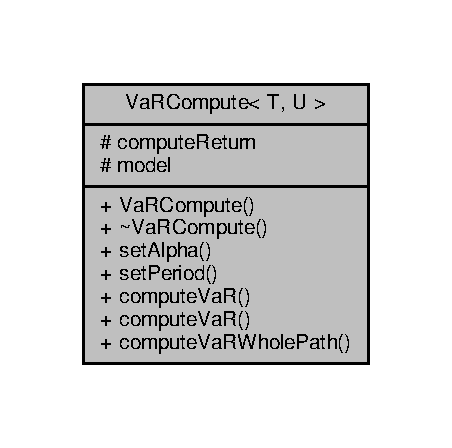
\includegraphics[width=217pt]{classVaRCompute__coll__graph}
\end{center}
\end{figure}
\subsection*{Public Member Functions}
\begin{DoxyCompactItemize}
\item 
\hyperlink{classVaRCompute_ac4fd50c6cb5cdc8ecd9964f1c317853a}{Va\+R\+Compute} (shared\+\_\+ptr$<$ T $>$ \&\+\_\+cr, const U \&\+\_\+model)
\item 
virtual \hyperlink{classVaRCompute_a18b310b3562cadd560a70e2614a0e09c}{$\sim$\+Va\+R\+Compute} ()
\item 
void \hyperlink{classVaRCompute_a9a58944ea61c92f90befb024d12fe80c}{set\+Alpha} (double alpha)
\item 
void \hyperlink{classVaRCompute_a071d01ccfd965e5a02d2ce4f3eee5db2}{set\+Period} (unsigned int period)
\item 
virtual double \hyperlink{classVaRCompute_a0465221010d248238fe1052958776984}{compute\+VaR} (size\+\_\+t p=0)=0
\begin{DoxyCompactList}\small\item\em compute \hyperlink{classVaR}{VaR} using whole path 1x overload \end{DoxyCompactList}\item 
double \hyperlink{classVaRCompute_a26618931d3370340944295ae5d882db5}{compute\+VaR} (double \+\_\+alpha, unsigned int \+\_\+period, unsigned \+\_\+k, size\+\_\+t p=0)
\item 
virtual std\+::vector$<$ double $>$ \hyperlink{classVaRCompute_ad5ec9feb42ea2f99f2c91e793d18fe1b}{compute\+Va\+R\+Whole\+Path} (size\+\_\+t p=0)=0
\end{DoxyCompactItemize}
\subsection*{Protected Attributes}
\begin{DoxyCompactItemize}
\item 
shared\+\_\+ptr$<$ T $>$ \hyperlink{classVaRCompute_a44d8fd1ac0cd7c920e1fc255f11a92ee}{compute\+Return}
\item 
U \hyperlink{classVaRCompute_a2de1fc8b4d4df387d0495981bde72564}{model}
\end{DoxyCompactItemize}


\subsection{Detailed Description}
\subsubsection*{template$<$class T, class U$>$\newline
class Va\+R\+Compute$<$ T, U $>$}

Compute \hyperlink{classVaR}{VaR}. 

\subsection{Constructor \& Destructor Documentation}
\hypertarget{classVaRCompute_ac4fd50c6cb5cdc8ecd9964f1c317853a}{}\label{classVaRCompute_ac4fd50c6cb5cdc8ecd9964f1c317853a} 
\index{Va\+R\+Compute@{Va\+R\+Compute}!Va\+R\+Compute@{Va\+R\+Compute}}
\index{Va\+R\+Compute@{Va\+R\+Compute}!Va\+R\+Compute@{Va\+R\+Compute}}
\subsubsection{\texorpdfstring{Va\+R\+Compute()}{VaRCompute()}}
{\footnotesize\ttfamily template$<$class T , class U $>$ \\
\hyperlink{classVaRCompute}{Va\+R\+Compute}$<$ T, U $>$\+::\hyperlink{classVaRCompute}{Va\+R\+Compute} (\begin{DoxyParamCaption}\item[{shared\+\_\+ptr$<$ T $>$ \&}]{\+\_\+cr,  }\item[{const U \&}]{\+\_\+model }\end{DoxyParamCaption})\hspace{0.3cm}{\ttfamily [inline]}}

\hypertarget{classVaRCompute_a18b310b3562cadd560a70e2614a0e09c}{}\label{classVaRCompute_a18b310b3562cadd560a70e2614a0e09c} 
\index{Va\+R\+Compute@{Va\+R\+Compute}!````~Va\+R\+Compute@{$\sim$\+Va\+R\+Compute}}
\index{````~Va\+R\+Compute@{$\sim$\+Va\+R\+Compute}!Va\+R\+Compute@{Va\+R\+Compute}}
\subsubsection{\texorpdfstring{$\sim$\+Va\+R\+Compute()}{~VaRCompute()}}
{\footnotesize\ttfamily template$<$class T , class U $>$ \\
virtual \hyperlink{classVaRCompute}{Va\+R\+Compute}$<$ T, U $>$\+::$\sim$\hyperlink{classVaRCompute}{Va\+R\+Compute} (\begin{DoxyParamCaption}{ }\end{DoxyParamCaption})\hspace{0.3cm}{\ttfamily [inline]}, {\ttfamily [virtual]}}



\subsection{Member Function Documentation}
\hypertarget{classVaRCompute_a0465221010d248238fe1052958776984}{}\label{classVaRCompute_a0465221010d248238fe1052958776984} 
\index{Va\+R\+Compute@{Va\+R\+Compute}!compute\+VaR@{compute\+VaR}}
\index{compute\+VaR@{compute\+VaR}!Va\+R\+Compute@{Va\+R\+Compute}}
\subsubsection{\texorpdfstring{compute\+Va\+R()}{computeVaR()}\hspace{0.1cm}{\footnotesize\ttfamily [1/2]}}
{\footnotesize\ttfamily template$<$class T , class U $>$ \\
virtual double \hyperlink{classVaRCompute}{Va\+R\+Compute}$<$ T, U $>$\+::compute\+VaR (\begin{DoxyParamCaption}\item[{size\+\_\+t}]{p = {\ttfamily 0} }\end{DoxyParamCaption})\hspace{0.3cm}{\ttfamily [pure virtual]}}



compute \hyperlink{classVaR}{VaR} using whole path 1x overload 



Implemented in \hyperlink{classVaRCopulaCompute_a5f2a4f1eab16cd600683309d49800e89}{Va\+R\+Copula\+Compute$<$ T, U, V $>$}, \hyperlink{classVaRMonteCarloCompute_a43b5493187d834fa2ba1bdb53c353947}{Va\+R\+Monte\+Carlo\+Compute$<$ T, U, V $>$}, \hyperlink{classVaRExtremeValueCompute_aa0a5cedce7a1a0dc0298f5b59add0e2c}{Va\+R\+Extreme\+Value\+Compute$<$ T, U $>$}, \hyperlink{classVaRnoneParamCompute_a171ea43cd1a1a9a38cf415c22e06898a}{Va\+Rnone\+Param\+Compute$<$ T, U $>$}, and \hyperlink{classVaRParamCompute_a0dcd8d0204328a73526aeb3859b3e159}{Va\+R\+Param\+Compute$<$ T, U $>$}.

\hypertarget{classVaRCompute_a26618931d3370340944295ae5d882db5}{}\label{classVaRCompute_a26618931d3370340944295ae5d882db5} 
\index{Va\+R\+Compute@{Va\+R\+Compute}!compute\+VaR@{compute\+VaR}}
\index{compute\+VaR@{compute\+VaR}!Va\+R\+Compute@{Va\+R\+Compute}}
\subsubsection{\texorpdfstring{compute\+Va\+R()}{computeVaR()}\hspace{0.1cm}{\footnotesize\ttfamily [2/2]}}
{\footnotesize\ttfamily template$<$class T , class U $>$ \\
double \hyperlink{classVaRCompute}{Va\+R\+Compute}$<$ T, U $>$\+::compute\+VaR (\begin{DoxyParamCaption}\item[{double}]{\+\_\+alpha,  }\item[{unsigned int}]{\+\_\+period,  }\item[{unsigned}]{\+\_\+k,  }\item[{size\+\_\+t}]{p = {\ttfamily 0} }\end{DoxyParamCaption})\hspace{0.3cm}{\ttfamily [inline]}}

\hypertarget{classVaRCompute_ad5ec9feb42ea2f99f2c91e793d18fe1b}{}\label{classVaRCompute_ad5ec9feb42ea2f99f2c91e793d18fe1b} 
\index{Va\+R\+Compute@{Va\+R\+Compute}!compute\+Va\+R\+Whole\+Path@{compute\+Va\+R\+Whole\+Path}}
\index{compute\+Va\+R\+Whole\+Path@{compute\+Va\+R\+Whole\+Path}!Va\+R\+Compute@{Va\+R\+Compute}}
\subsubsection{\texorpdfstring{compute\+Va\+R\+Whole\+Path()}{computeVaRWholePath()}}
{\footnotesize\ttfamily template$<$class T , class U $>$ \\
virtual std\+::vector$<$double$>$ \hyperlink{classVaRCompute}{Va\+R\+Compute}$<$ T, U $>$\+::compute\+Va\+R\+Whole\+Path (\begin{DoxyParamCaption}\item[{size\+\_\+t}]{p = {\ttfamily 0} }\end{DoxyParamCaption})\hspace{0.3cm}{\ttfamily [pure virtual]}}



Implemented in \hyperlink{classVaRCopulaCompute_a6c2501fcfd848a07a91859f2bcdc6516}{Va\+R\+Copula\+Compute$<$ T, U, V $>$}, \hyperlink{classVaRMonteCarloCompute_a14ea83586172f23f8bb4a60babeb812f}{Va\+R\+Monte\+Carlo\+Compute$<$ T, U, V $>$}, \hyperlink{classVaRExtremeValueCompute_ad3b7ec9abcd6f6b27c89cf77e0099d18}{Va\+R\+Extreme\+Value\+Compute$<$ T, U $>$}, \hyperlink{classVaRnoneParamCompute_a7ddfb62c4e1e9890542818c75c51798e}{Va\+Rnone\+Param\+Compute$<$ T, U $>$}, and \hyperlink{classVaRParamCompute_abc97057d7e35d8dc98fb3a560be67d0d}{Va\+R\+Param\+Compute$<$ T, U $>$}.

\hypertarget{classVaRCompute_a9a58944ea61c92f90befb024d12fe80c}{}\label{classVaRCompute_a9a58944ea61c92f90befb024d12fe80c} 
\index{Va\+R\+Compute@{Va\+R\+Compute}!set\+Alpha@{set\+Alpha}}
\index{set\+Alpha@{set\+Alpha}!Va\+R\+Compute@{Va\+R\+Compute}}
\subsubsection{\texorpdfstring{set\+Alpha()}{setAlpha()}}
{\footnotesize\ttfamily template$<$class T , class U $>$ \\
void \hyperlink{classVaRCompute}{Va\+R\+Compute}$<$ T, U $>$\+::set\+Alpha (\begin{DoxyParamCaption}\item[{double}]{alpha }\end{DoxyParamCaption})\hspace{0.3cm}{\ttfamily [inline]}}

\hypertarget{classVaRCompute_a071d01ccfd965e5a02d2ce4f3eee5db2}{}\label{classVaRCompute_a071d01ccfd965e5a02d2ce4f3eee5db2} 
\index{Va\+R\+Compute@{Va\+R\+Compute}!set\+Period@{set\+Period}}
\index{set\+Period@{set\+Period}!Va\+R\+Compute@{Va\+R\+Compute}}
\subsubsection{\texorpdfstring{set\+Period()}{setPeriod()}}
{\footnotesize\ttfamily template$<$class T , class U $>$ \\
void \hyperlink{classVaRCompute}{Va\+R\+Compute}$<$ T, U $>$\+::set\+Period (\begin{DoxyParamCaption}\item[{unsigned int}]{period }\end{DoxyParamCaption})\hspace{0.3cm}{\ttfamily [inline]}}



\subsection{Member Data Documentation}
\hypertarget{classVaRCompute_a44d8fd1ac0cd7c920e1fc255f11a92ee}{}\label{classVaRCompute_a44d8fd1ac0cd7c920e1fc255f11a92ee} 
\index{Va\+R\+Compute@{Va\+R\+Compute}!compute\+Return@{compute\+Return}}
\index{compute\+Return@{compute\+Return}!Va\+R\+Compute@{Va\+R\+Compute}}
\subsubsection{\texorpdfstring{compute\+Return}{computeReturn}}
{\footnotesize\ttfamily template$<$class T , class U $>$ \\
shared\+\_\+ptr$<$T$>$ \hyperlink{classVaRCompute}{Va\+R\+Compute}$<$ T, U $>$\+::compute\+Return\hspace{0.3cm}{\ttfamily [protected]}}

\hypertarget{classVaRCompute_a2de1fc8b4d4df387d0495981bde72564}{}\label{classVaRCompute_a2de1fc8b4d4df387d0495981bde72564} 
\index{Va\+R\+Compute@{Va\+R\+Compute}!model@{model}}
\index{model@{model}!Va\+R\+Compute@{Va\+R\+Compute}}
\subsubsection{\texorpdfstring{model}{model}}
{\footnotesize\ttfamily template$<$class T , class U $>$ \\
U \hyperlink{classVaRCompute}{Va\+R\+Compute}$<$ T, U $>$\+::model\hspace{0.3cm}{\ttfamily [protected]}}



The documentation for this class was generated from the following file\+:\begin{DoxyCompactItemize}
\item 
\hyperlink{compute__var_8h}{compute\+\_\+var.\+h}\end{DoxyCompactItemize}

\hypertarget{classVaRCopulaCompute}{}\section{Va\+R\+Copula\+Compute$<$ T, U, V $>$ Class Template Reference}
\label{classVaRCopulaCompute}\index{Va\+R\+Copula\+Compute$<$ T, U, V $>$@{Va\+R\+Copula\+Compute$<$ T, U, V $>$}}


Compute \hyperlink{classVaR}{VaR} using Monte Carlo \& Copula.  




{\ttfamily \#include $<$compute\+\_\+var.\+h$>$}



Inheritance diagram for Va\+R\+Copula\+Compute$<$ T, U, V $>$\+:
\nopagebreak
\begin{figure}[H]
\begin{center}
\leavevmode
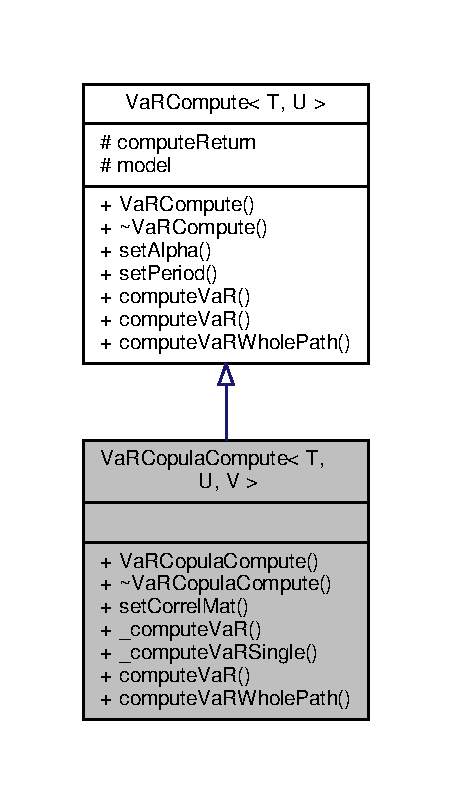
\includegraphics[width=217pt]{classVaRCopulaCompute__inherit__graph}
\end{center}
\end{figure}


Collaboration diagram for Va\+R\+Copula\+Compute$<$ T, U, V $>$\+:
\nopagebreak
\begin{figure}[H]
\begin{center}
\leavevmode
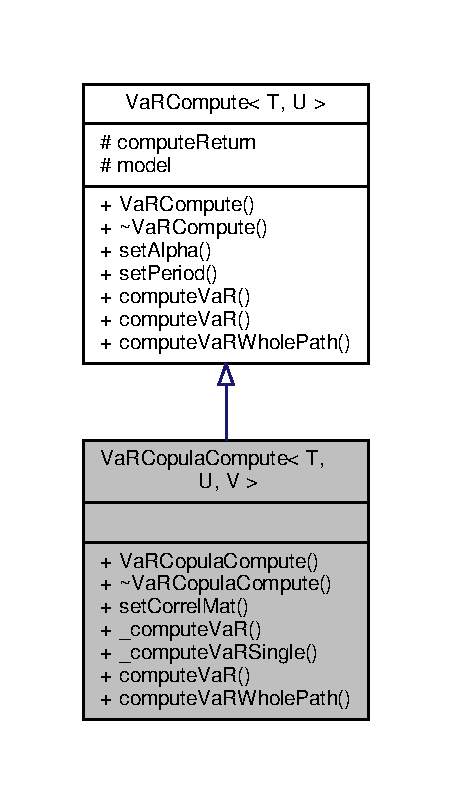
\includegraphics[width=217pt]{classVaRCopulaCompute__coll__graph}
\end{center}
\end{figure}
\subsection*{Public Types}
\begin{DoxyCompactItemize}
\item 
typedef \hyperlink{classCopulaEngine}{Copula\+Engine}$<$ \hyperlink{classrng}{rng}, V $>$ \hyperlink{classVaRCopulaCompute_a72e41ad9fcb5880aac35affa027f2e3d}{engine}
\end{DoxyCompactItemize}
\subsection*{Public Member Functions}
\begin{DoxyCompactItemize}
\item 
\hyperlink{classVaRCopulaCompute_a5e9c7b93130a65cbf5006fccb861c235}{Va\+R\+Copula\+Compute} (shared\+\_\+ptr$<$ T $>$ \&\+\_\+cr, const U \&\+\_\+model, const std\+::vector$<$ V $>$ \&\+\_\+processes, \hyperlink{classrng}{rng} \&\+\_\+rng\+\_\+, const Eigen\+::\+Matrix\+Xd \&\+\_\+C, const double \&\+\_\+n=1.e+05)
\item 
virtual \hyperlink{classVaRCopulaCompute_a3f31ae6973366895926f6b3ae11ef473}{$\sim$\+Va\+R\+Copula\+Compute} ()
\item 
void \hyperlink{classVaRCopulaCompute_a8263b7ec27286cee0a65019c9a90f51d}{set\+Correl\+Mat} (const Eigen\+::\+Matrix\+Xd \&\+\_\+C)
\item 
\hyperlink{compute__returns__eigen_8h_a1eb6a9306ef406d7975f3cbf2e247777}{Vec} \hyperlink{classVaRCopulaCompute_a367ca6f0e63ef6bb493d732435fc9b8d}{\+\_\+compute\+VaR} (double dof=3., double gamma=1., \hyperlink{rng_8h_aff2c6be1fded3d6d996b850e2eb87c25}{copula\+Type} ct=\hyperlink{rng_8h_aff2c6be1fded3d6d996b850e2eb87c25ab15a7891aa5223439e4692a1048cb220}{Gauss}, \hyperlink{mc__engine_8h_aeb3b337d49b67199ac031f705d206198}{underlying\+Process} ud=\hyperlink{mc__engine_8h_aeb3b337d49b67199ac031f705d206198aa11844f44df96808eb4e519ba04f088c}{Gaussian}, size\+\_\+t a=0, size\+\_\+t b=1)
\begin{DoxyCompactList}\small\item\em Compute \hyperlink{classVaR}{VaR} using Monte Carlo simulation from either Gaussian or Student\textquotesingle{}s t distr. \end{DoxyCompactList}\item 
double \hyperlink{classVaRCopulaCompute_a526b139c60a9f014b0e03eeae9d0f098}{\+\_\+compute\+Va\+R\+Single} (size\+\_\+t p=0, double dof=3., double gamma=1., \hyperlink{rng_8h_aff2c6be1fded3d6d996b850e2eb87c25}{copula\+Type} ct=\hyperlink{rng_8h_aff2c6be1fded3d6d996b850e2eb87c25ab15a7891aa5223439e4692a1048cb220}{Gauss}, \hyperlink{mc__engine_8h_aeb3b337d49b67199ac031f705d206198}{underlying\+Process} ud=\hyperlink{mc__engine_8h_aeb3b337d49b67199ac031f705d206198aa11844f44df96808eb4e519ba04f088c}{Gaussian}, size\+\_\+t a=0, size\+\_\+t b=1)
\begin{DoxyCompactList}\small\item\em Compute \hyperlink{classVaR}{VaR} using Monte Carlo simulation from either Gaussian or Student\textquotesingle{}s t distr. \end{DoxyCompactList}\item 
double \hyperlink{classVaRCopulaCompute_a5f2a4f1eab16cd600683309d49800e89}{compute\+VaR} (size\+\_\+t p=0)
\begin{DoxyCompactList}\small\item\em Compute for security, index, etc p. \end{DoxyCompactList}\item 
std\+::vector$<$ double $>$ \hyperlink{classVaRCopulaCompute_a6c2501fcfd848a07a91859f2bcdc6516}{compute\+Va\+R\+Whole\+Path} (size\+\_\+t p=0)
\begin{DoxyCompactList}\small\item\em Compute \hyperlink{classVaR}{VaR} over whole path. \end{DoxyCompactList}\end{DoxyCompactItemize}
\subsection*{Additional Inherited Members}


\subsection{Detailed Description}
\subsubsection*{template$<$class T, class U, class V$>$\newline
class Va\+R\+Copula\+Compute$<$ T, U, V $>$}

Compute \hyperlink{classVaR}{VaR} using Monte Carlo \& Copula. 

compute \hyperlink{classVaR}{VaR} using sim returns and histogram method 

\subsection{Member Typedef Documentation}
\hypertarget{classVaRCopulaCompute_a72e41ad9fcb5880aac35affa027f2e3d}{}\label{classVaRCopulaCompute_a72e41ad9fcb5880aac35affa027f2e3d} 
\index{Va\+R\+Copula\+Compute@{Va\+R\+Copula\+Compute}!engine@{engine}}
\index{engine@{engine}!Va\+R\+Copula\+Compute@{Va\+R\+Copula\+Compute}}
\subsubsection{\texorpdfstring{engine}{engine}}
{\footnotesize\ttfamily template$<$class T , class U , class V $>$ \\
typedef \hyperlink{classCopulaEngine}{Copula\+Engine}$<$\hyperlink{classrng}{rng},V$>$ \hyperlink{classVaRCopulaCompute}{Va\+R\+Copula\+Compute}$<$ T, U, V $>$\+::\hyperlink{classVaRCopulaCompute_a72e41ad9fcb5880aac35affa027f2e3d}{engine}}



\subsection{Constructor \& Destructor Documentation}
\hypertarget{classVaRCopulaCompute_a5e9c7b93130a65cbf5006fccb861c235}{}\label{classVaRCopulaCompute_a5e9c7b93130a65cbf5006fccb861c235} 
\index{Va\+R\+Copula\+Compute@{Va\+R\+Copula\+Compute}!Va\+R\+Copula\+Compute@{Va\+R\+Copula\+Compute}}
\index{Va\+R\+Copula\+Compute@{Va\+R\+Copula\+Compute}!Va\+R\+Copula\+Compute@{Va\+R\+Copula\+Compute}}
\subsubsection{\texorpdfstring{Va\+R\+Copula\+Compute()}{VaRCopulaCompute()}}
{\footnotesize\ttfamily template$<$class T , class U , class V $>$ \\
\hyperlink{classVaRCopulaCompute}{Va\+R\+Copula\+Compute}$<$ T, U, V $>$\+::\hyperlink{classVaRCopulaCompute}{Va\+R\+Copula\+Compute} (\begin{DoxyParamCaption}\item[{shared\+\_\+ptr$<$ T $>$ \&}]{\+\_\+cr,  }\item[{const U \&}]{\+\_\+model,  }\item[{const std\+::vector$<$ V $>$ \&}]{\+\_\+processes,  }\item[{\hyperlink{classrng}{rng} \&}]{\+\_\+rng\+\_\+,  }\item[{const Eigen\+::\+Matrix\+Xd \&}]{\+\_\+C,  }\item[{const double \&}]{\+\_\+n = {\ttfamily 1.e+05} }\end{DoxyParamCaption})\hspace{0.3cm}{\ttfamily [inline]}}


\begin{DoxyParams}{Parameters}
{\em \+\_\+cr} & compute return class \\
\hline
{\em \+\_\+model} & \hyperlink{classVaR}{VaR} model \\
\hline
{\em \+\_\+process} & underlying process \\
\hline
{\em C} & correlation matrix of standardized residuals \\
\hline
{\em n} & \# of simulation draws \\
\hline
\end{DoxyParams}
\hypertarget{classVaRCopulaCompute_a3f31ae6973366895926f6b3ae11ef473}{}\label{classVaRCopulaCompute_a3f31ae6973366895926f6b3ae11ef473} 
\index{Va\+R\+Copula\+Compute@{Va\+R\+Copula\+Compute}!````~Va\+R\+Copula\+Compute@{$\sim$\+Va\+R\+Copula\+Compute}}
\index{````~Va\+R\+Copula\+Compute@{$\sim$\+Va\+R\+Copula\+Compute}!Va\+R\+Copula\+Compute@{Va\+R\+Copula\+Compute}}
\subsubsection{\texorpdfstring{$\sim$\+Va\+R\+Copula\+Compute()}{~VaRCopulaCompute()}}
{\footnotesize\ttfamily template$<$class T , class U , class V $>$ \\
virtual \hyperlink{classVaRCopulaCompute}{Va\+R\+Copula\+Compute}$<$ T, U, V $>$\+::$\sim$\hyperlink{classVaRCopulaCompute}{Va\+R\+Copula\+Compute} (\begin{DoxyParamCaption}{ }\end{DoxyParamCaption})\hspace{0.3cm}{\ttfamily [inline]}, {\ttfamily [virtual]}}



\subsection{Member Function Documentation}
\hypertarget{classVaRCopulaCompute_a367ca6f0e63ef6bb493d732435fc9b8d}{}\label{classVaRCopulaCompute_a367ca6f0e63ef6bb493d732435fc9b8d} 
\index{Va\+R\+Copula\+Compute@{Va\+R\+Copula\+Compute}!\+\_\+compute\+VaR@{\+\_\+compute\+VaR}}
\index{\+\_\+compute\+VaR@{\+\_\+compute\+VaR}!Va\+R\+Copula\+Compute@{Va\+R\+Copula\+Compute}}
\subsubsection{\texorpdfstring{\+\_\+compute\+Va\+R()}{\_computeVaR()}}
{\footnotesize\ttfamily template$<$class T , class U , class V $>$ \\
\hyperlink{compute__returns__eigen_8h_a1eb6a9306ef406d7975f3cbf2e247777}{Vec} \hyperlink{classVaRCopulaCompute}{Va\+R\+Copula\+Compute}$<$ T, U, V $>$\+::\+\_\+compute\+VaR (\begin{DoxyParamCaption}\item[{double}]{dof = {\ttfamily 3.},  }\item[{double}]{gamma = {\ttfamily 1.},  }\item[{\hyperlink{rng_8h_aff2c6be1fded3d6d996b850e2eb87c25}{copula\+Type}}]{ct = {\ttfamily \hyperlink{rng_8h_aff2c6be1fded3d6d996b850e2eb87c25ab15a7891aa5223439e4692a1048cb220}{Gauss}},  }\item[{\hyperlink{mc__engine_8h_aeb3b337d49b67199ac031f705d206198}{underlying\+Process}}]{ud = {\ttfamily \hyperlink{mc__engine_8h_aeb3b337d49b67199ac031f705d206198aa11844f44df96808eb4e519ba04f088c}{Gaussian}},  }\item[{size\+\_\+t}]{a = {\ttfamily 0},  }\item[{size\+\_\+t}]{b = {\ttfamily 1} }\end{DoxyParamCaption})\hspace{0.3cm}{\ttfamily [inline]}}



Compute \hyperlink{classVaR}{VaR} using Monte Carlo simulation from either Gaussian or Student\textquotesingle{}s t distr. 


\begin{DoxyParams}{Parameters}
{\em dof} & degree of freedom \\
\hline
{\em copula\+Type} & Gaussian, Student\textquotesingle{}s t, Clayton, Gumbel \\
\hline
{\em underlying\+Mar} & Gaussian, Student\textquotesingle{}s t \\
\hline
{\em a} & param time t-\/1. Default 0 \\
\hline
{\em b} & param time t. Default 1\\
\hline
\end{DoxyParams}
\begin{DoxyReturn}{Returns}
Return vectors of Va\+Rs of dimension d 
\end{DoxyReturn}
\hypertarget{classVaRCopulaCompute_a526b139c60a9f014b0e03eeae9d0f098}{}\label{classVaRCopulaCompute_a526b139c60a9f014b0e03eeae9d0f098} 
\index{Va\+R\+Copula\+Compute@{Va\+R\+Copula\+Compute}!\+\_\+compute\+Va\+R\+Single@{\+\_\+compute\+Va\+R\+Single}}
\index{\+\_\+compute\+Va\+R\+Single@{\+\_\+compute\+Va\+R\+Single}!Va\+R\+Copula\+Compute@{Va\+R\+Copula\+Compute}}
\subsubsection{\texorpdfstring{\+\_\+compute\+Va\+R\+Single()}{\_computeVaRSingle()}}
{\footnotesize\ttfamily template$<$class T , class U , class V $>$ \\
double \hyperlink{classVaRCopulaCompute}{Va\+R\+Copula\+Compute}$<$ T, U, V $>$\+::\+\_\+compute\+Va\+R\+Single (\begin{DoxyParamCaption}\item[{size\+\_\+t}]{p = {\ttfamily 0},  }\item[{double}]{dof = {\ttfamily 3.},  }\item[{double}]{gamma = {\ttfamily 1.},  }\item[{\hyperlink{rng_8h_aff2c6be1fded3d6d996b850e2eb87c25}{copula\+Type}}]{ct = {\ttfamily \hyperlink{rng_8h_aff2c6be1fded3d6d996b850e2eb87c25ab15a7891aa5223439e4692a1048cb220}{Gauss}},  }\item[{\hyperlink{mc__engine_8h_aeb3b337d49b67199ac031f705d206198}{underlying\+Process}}]{ud = {\ttfamily \hyperlink{mc__engine_8h_aeb3b337d49b67199ac031f705d206198aa11844f44df96808eb4e519ba04f088c}{Gaussian}},  }\item[{size\+\_\+t}]{a = {\ttfamily 0},  }\item[{size\+\_\+t}]{b = {\ttfamily 1} }\end{DoxyParamCaption})\hspace{0.3cm}{\ttfamily [inline]}}



Compute \hyperlink{classVaR}{VaR} using Monte Carlo simulation from either Gaussian or Student\textquotesingle{}s t distr. 


\begin{DoxyParams}{Parameters}
{\em p} & procees p. Default 0 \\
\hline
{\em dof} & degree of freedom \\
\hline
{\em copula\+Type} & Gaussian, Student\textquotesingle{}s t, Clayton, Gumbel \\
\hline
{\em underlying\+Mar} & Gaussian, Student\textquotesingle{}s t \\
\hline
{\em a} & param time t-\/1. Default 0 \\
\hline
{\em b} & param time t. Default 1\\
\hline
\end{DoxyParams}
\begin{DoxyReturn}{Returns}
Va\+Rs for process p 
\end{DoxyReturn}
\hypertarget{classVaRCopulaCompute_a5f2a4f1eab16cd600683309d49800e89}{}\label{classVaRCopulaCompute_a5f2a4f1eab16cd600683309d49800e89} 
\index{Va\+R\+Copula\+Compute@{Va\+R\+Copula\+Compute}!compute\+VaR@{compute\+VaR}}
\index{compute\+VaR@{compute\+VaR}!Va\+R\+Copula\+Compute@{Va\+R\+Copula\+Compute}}
\subsubsection{\texorpdfstring{compute\+Va\+R()}{computeVaR()}}
{\footnotesize\ttfamily template$<$class T , class U , class V $>$ \\
double \hyperlink{classVaRCopulaCompute}{Va\+R\+Copula\+Compute}$<$ T, U, V $>$\+::compute\+VaR (\begin{DoxyParamCaption}\item[{size\+\_\+t}]{p = {\ttfamily 0} }\end{DoxyParamCaption})\hspace{0.3cm}{\ttfamily [inline]}, {\ttfamily [virtual]}}



Compute for security, index, etc p. 

Assume t-\/copula with 3 degrees of freedom 

Implements \hyperlink{classVaRCompute_a0465221010d248238fe1052958776984}{Va\+R\+Compute$<$ T, U $>$}.

\hypertarget{classVaRCopulaCompute_a6c2501fcfd848a07a91859f2bcdc6516}{}\label{classVaRCopulaCompute_a6c2501fcfd848a07a91859f2bcdc6516} 
\index{Va\+R\+Copula\+Compute@{Va\+R\+Copula\+Compute}!compute\+Va\+R\+Whole\+Path@{compute\+Va\+R\+Whole\+Path}}
\index{compute\+Va\+R\+Whole\+Path@{compute\+Va\+R\+Whole\+Path}!Va\+R\+Copula\+Compute@{Va\+R\+Copula\+Compute}}
\subsubsection{\texorpdfstring{compute\+Va\+R\+Whole\+Path()}{computeVaRWholePath()}}
{\footnotesize\ttfamily template$<$class T , class U , class V $>$ \\
std\+::vector$<$double$>$ \hyperlink{classVaRCopulaCompute}{Va\+R\+Copula\+Compute}$<$ T, U, V $>$\+::compute\+Va\+R\+Whole\+Path (\begin{DoxyParamCaption}\item[{size\+\_\+t}]{p = {\ttfamily 0} }\end{DoxyParamCaption})\hspace{0.3cm}{\ttfamily [inline]}, {\ttfamily [virtual]}}



Compute \hyperlink{classVaR}{VaR} over whole path. 

Assume t-\/copula with 3 degrees of freedom. Reduce n to 1e+04 

Implements \hyperlink{classVaRCompute_ad5ec9feb42ea2f99f2c91e793d18fe1b}{Va\+R\+Compute$<$ T, U $>$}.

\hypertarget{classVaRCopulaCompute_a8263b7ec27286cee0a65019c9a90f51d}{}\label{classVaRCopulaCompute_a8263b7ec27286cee0a65019c9a90f51d} 
\index{Va\+R\+Copula\+Compute@{Va\+R\+Copula\+Compute}!set\+Correl\+Mat@{set\+Correl\+Mat}}
\index{set\+Correl\+Mat@{set\+Correl\+Mat}!Va\+R\+Copula\+Compute@{Va\+R\+Copula\+Compute}}
\subsubsection{\texorpdfstring{set\+Correl\+Mat()}{setCorrelMat()}}
{\footnotesize\ttfamily template$<$class T , class U , class V $>$ \\
void \hyperlink{classVaRCopulaCompute}{Va\+R\+Copula\+Compute}$<$ T, U, V $>$\+::set\+Correl\+Mat (\begin{DoxyParamCaption}\item[{const Eigen\+::\+Matrix\+Xd \&}]{\+\_\+C }\end{DoxyParamCaption})\hspace{0.3cm}{\ttfamily [inline]}}



The documentation for this class was generated from the following file\+:\begin{DoxyCompactItemize}
\item 
\hyperlink{compute__var_8h}{compute\+\_\+var.\+h}\end{DoxyCompactItemize}

\hypertarget{classVaRExtremeValueCompute}{}\section{Va\+R\+Extreme\+Value\+Compute$<$ T, U $>$ Class Template Reference}
\label{classVaRExtremeValueCompute}\index{Va\+R\+Extreme\+Value\+Compute$<$ T, U $>$@{Va\+R\+Extreme\+Value\+Compute$<$ T, U $>$}}


Compute \hyperlink{classVaR}{VaR} using extreme value -\/ Generalized Pareto.  




{\ttfamily \#include $<$compute\+\_\+var.\+h$>$}



Inheritance diagram for Va\+R\+Extreme\+Value\+Compute$<$ T, U $>$\+:
\nopagebreak
\begin{figure}[H]
\begin{center}
\leavevmode
\includegraphics[width=238pt]{classVaRExtremeValueCompute__inherit__graph}
\end{center}
\end{figure}


Collaboration diagram for Va\+R\+Extreme\+Value\+Compute$<$ T, U $>$\+:
\nopagebreak
\begin{figure}[H]
\begin{center}
\leavevmode
\includegraphics[width=238pt]{classVaRExtremeValueCompute__coll__graph}
\end{center}
\end{figure}
\subsection*{Public Member Functions}
\begin{DoxyCompactItemize}
\item 
\hyperlink{classVaRExtremeValueCompute_ac6a44f45d19035602c3bf885466597bb}{Va\+R\+Extreme\+Value\+Compute} (shared\+\_\+ptr$<$ T $>$ \&\+\_\+cr, const U \&\+\_\+model)
\item 
virtual \hyperlink{classVaRExtremeValueCompute_a84bce72bd46b30a48fc6e86bb72201f9}{$\sim$\+Va\+R\+Extreme\+Value\+Compute} ()
\item 
double \hyperlink{classVaRExtremeValueCompute_aa0a5cedce7a1a0dc0298f5b59add0e2c}{compute\+VaR} (size\+\_\+t p=0)
\begin{DoxyCompactList}\small\item\em compute \hyperlink{classVaR}{VaR} using whole path 1x overload \end{DoxyCompactList}\item 
double \hyperlink{classVaRExtremeValueCompute_afa071fb24b112d282847f8ad6732060f}{compute\+ES} (size\+\_\+t p=0)
\item 
std\+::vector$<$ double $>$ \hyperlink{classVaRExtremeValueCompute_ad3b7ec9abcd6f6b27c89cf77e0099d18}{compute\+Va\+R\+Whole\+Path} (size\+\_\+t p=0)
\begin{DoxyCompactList}\small\item\em compute \hyperlink{classVaR}{VaR} over whole path \end{DoxyCompactList}\end{DoxyCompactItemize}
\subsection*{Additional Inherited Members}


\subsection{Detailed Description}
\subsubsection*{template$<$class T, class U$>$\newline
class Va\+R\+Extreme\+Value\+Compute$<$ T, U $>$}

Compute \hyperlink{classVaR}{VaR} using extreme value -\/ Generalized Pareto. 

\subsection{Constructor \& Destructor Documentation}
\hypertarget{classVaRExtremeValueCompute_ac6a44f45d19035602c3bf885466597bb}{}\label{classVaRExtremeValueCompute_ac6a44f45d19035602c3bf885466597bb} 
\index{Va\+R\+Extreme\+Value\+Compute@{Va\+R\+Extreme\+Value\+Compute}!Va\+R\+Extreme\+Value\+Compute@{Va\+R\+Extreme\+Value\+Compute}}
\index{Va\+R\+Extreme\+Value\+Compute@{Va\+R\+Extreme\+Value\+Compute}!Va\+R\+Extreme\+Value\+Compute@{Va\+R\+Extreme\+Value\+Compute}}
\subsubsection{\texorpdfstring{Va\+R\+Extreme\+Value\+Compute()}{VaRExtremeValueCompute()}}
{\footnotesize\ttfamily template$<$class T , class U $>$ \\
\hyperlink{classVaRExtremeValueCompute}{Va\+R\+Extreme\+Value\+Compute}$<$ T, U $>$\+::\hyperlink{classVaRExtremeValueCompute}{Va\+R\+Extreme\+Value\+Compute} (\begin{DoxyParamCaption}\item[{shared\+\_\+ptr$<$ T $>$ \&}]{\+\_\+cr,  }\item[{const U \&}]{\+\_\+model }\end{DoxyParamCaption})\hspace{0.3cm}{\ttfamily [inline]}}

\hypertarget{classVaRExtremeValueCompute_a84bce72bd46b30a48fc6e86bb72201f9}{}\label{classVaRExtremeValueCompute_a84bce72bd46b30a48fc6e86bb72201f9} 
\index{Va\+R\+Extreme\+Value\+Compute@{Va\+R\+Extreme\+Value\+Compute}!````~Va\+R\+Extreme\+Value\+Compute@{$\sim$\+Va\+R\+Extreme\+Value\+Compute}}
\index{````~Va\+R\+Extreme\+Value\+Compute@{$\sim$\+Va\+R\+Extreme\+Value\+Compute}!Va\+R\+Extreme\+Value\+Compute@{Va\+R\+Extreme\+Value\+Compute}}
\subsubsection{\texorpdfstring{$\sim$\+Va\+R\+Extreme\+Value\+Compute()}{~VaRExtremeValueCompute()}}
{\footnotesize\ttfamily template$<$class T , class U $>$ \\
virtual \hyperlink{classVaRExtremeValueCompute}{Va\+R\+Extreme\+Value\+Compute}$<$ T, U $>$\+::$\sim$\hyperlink{classVaRExtremeValueCompute}{Va\+R\+Extreme\+Value\+Compute} (\begin{DoxyParamCaption}{ }\end{DoxyParamCaption})\hspace{0.3cm}{\ttfamily [inline]}, {\ttfamily [virtual]}}



\subsection{Member Function Documentation}
\hypertarget{classVaRExtremeValueCompute_afa071fb24b112d282847f8ad6732060f}{}\label{classVaRExtremeValueCompute_afa071fb24b112d282847f8ad6732060f} 
\index{Va\+R\+Extreme\+Value\+Compute@{Va\+R\+Extreme\+Value\+Compute}!compute\+ES@{compute\+ES}}
\index{compute\+ES@{compute\+ES}!Va\+R\+Extreme\+Value\+Compute@{Va\+R\+Extreme\+Value\+Compute}}
\subsubsection{\texorpdfstring{compute\+E\+S()}{computeES()}}
{\footnotesize\ttfamily template$<$class T , class U $>$ \\
double \hyperlink{classVaRExtremeValueCompute}{Va\+R\+Extreme\+Value\+Compute}$<$ T, U $>$\+::compute\+ES (\begin{DoxyParamCaption}\item[{size\+\_\+t}]{p = {\ttfamily 0} }\end{DoxyParamCaption})\hspace{0.3cm}{\ttfamily [inline]}}

\hypertarget{classVaRExtremeValueCompute_aa0a5cedce7a1a0dc0298f5b59add0e2c}{}\label{classVaRExtremeValueCompute_aa0a5cedce7a1a0dc0298f5b59add0e2c} 
\index{Va\+R\+Extreme\+Value\+Compute@{Va\+R\+Extreme\+Value\+Compute}!compute\+VaR@{compute\+VaR}}
\index{compute\+VaR@{compute\+VaR}!Va\+R\+Extreme\+Value\+Compute@{Va\+R\+Extreme\+Value\+Compute}}
\subsubsection{\texorpdfstring{compute\+Va\+R()}{computeVaR()}}
{\footnotesize\ttfamily template$<$class T , class U $>$ \\
double \hyperlink{classVaRExtremeValueCompute}{Va\+R\+Extreme\+Value\+Compute}$<$ T, U $>$\+::compute\+VaR (\begin{DoxyParamCaption}\item[{size\+\_\+t}]{p = {\ttfamily 0} }\end{DoxyParamCaption})\hspace{0.3cm}{\ttfamily [inline]}, {\ttfamily [virtual]}}



compute \hyperlink{classVaR}{VaR} using whole path 1x overload 



Implements \hyperlink{classVaRCompute_a0465221010d248238fe1052958776984}{Va\+R\+Compute$<$ T, U $>$}.

\hypertarget{classVaRExtremeValueCompute_ad3b7ec9abcd6f6b27c89cf77e0099d18}{}\label{classVaRExtremeValueCompute_ad3b7ec9abcd6f6b27c89cf77e0099d18} 
\index{Va\+R\+Extreme\+Value\+Compute@{Va\+R\+Extreme\+Value\+Compute}!compute\+Va\+R\+Whole\+Path@{compute\+Va\+R\+Whole\+Path}}
\index{compute\+Va\+R\+Whole\+Path@{compute\+Va\+R\+Whole\+Path}!Va\+R\+Extreme\+Value\+Compute@{Va\+R\+Extreme\+Value\+Compute}}
\subsubsection{\texorpdfstring{compute\+Va\+R\+Whole\+Path()}{computeVaRWholePath()}}
{\footnotesize\ttfamily template$<$class T , class U $>$ \\
std\+::vector$<$double$>$ \hyperlink{classVaRExtremeValueCompute}{Va\+R\+Extreme\+Value\+Compute}$<$ T, U $>$\+::compute\+Va\+R\+Whole\+Path (\begin{DoxyParamCaption}\item[{size\+\_\+t}]{p = {\ttfamily 0} }\end{DoxyParamCaption})\hspace{0.3cm}{\ttfamily [inline]}, {\ttfamily [virtual]}}



compute \hyperlink{classVaR}{VaR} over whole path 



Implements \hyperlink{classVaRCompute_ad5ec9feb42ea2f99f2c91e793d18fe1b}{Va\+R\+Compute$<$ T, U $>$}.



The documentation for this class was generated from the following file\+:\begin{DoxyCompactItemize}
\item 
\hyperlink{compute__var_8h}{compute\+\_\+var.\+h}\end{DoxyCompactItemize}

\hypertarget{classVaRMonteCarloCompute}{}\section{Va\+R\+Monte\+Carlo\+Compute$<$ T, U, V $>$ Class Template Reference}
\label{classVaRMonteCarloCompute}\index{Va\+R\+Monte\+Carlo\+Compute$<$ T, U, V $>$@{Va\+R\+Monte\+Carlo\+Compute$<$ T, U, V $>$}}


Compute \hyperlink{classVaR}{VaR} using Monte Carlo.  




{\ttfamily \#include $<$compute\+\_\+var.\+h$>$}



Inheritance diagram for Va\+R\+Monte\+Carlo\+Compute$<$ T, U, V $>$\+:
\nopagebreak
\begin{figure}[H]
\begin{center}
\leavevmode
\includegraphics[width=227pt]{classVaRMonteCarloCompute__inherit__graph}
\end{center}
\end{figure}


Collaboration diagram for Va\+R\+Monte\+Carlo\+Compute$<$ T, U, V $>$\+:
\nopagebreak
\begin{figure}[H]
\begin{center}
\leavevmode
\includegraphics[width=227pt]{classVaRMonteCarloCompute__coll__graph}
\end{center}
\end{figure}
\subsection*{Public Types}
\begin{DoxyCompactItemize}
\item 
typedef \hyperlink{classMCEngine}{M\+C\+Engine}$<$ \hyperlink{classrng}{rng}, V $>$ \hyperlink{classVaRMonteCarloCompute_a7ab31736fcc0c8c0630232d522186250}{engine}
\end{DoxyCompactItemize}
\subsection*{Public Member Functions}
\begin{DoxyCompactItemize}
\item 
\hyperlink{classVaRMonteCarloCompute_a2362734a7d6eb5530984ace252361a6a}{Va\+R\+Monte\+Carlo\+Compute} (shared\+\_\+ptr$<$ T $>$ \&\+\_\+cr, const U \&\+\_\+model, const V \&\+\_\+process, \hyperlink{classrng}{rng} \&\+\_\+rng, const double \&\+\_\+n=1.e+05)
\item 
virtual \hyperlink{classVaRMonteCarloCompute_a372e6887ccaab471a23c49b3e7868fa5}{$\sim$\+Va\+R\+Monte\+Carlo\+Compute} ()
\item 
void \hyperlink{classVaRMonteCarloCompute_a3ef6b8ac6e54e0dc4cc8239926d8f236}{set\+Numberof\+Sim} (double \+\_\+n)
\item 
double \hyperlink{classVaRMonteCarloCompute_a43b5493187d834fa2ba1bdb53c353947}{compute\+VaR} (size\+\_\+t p=0)
\begin{DoxyCompactList}\small\item\em Compute \hyperlink{classVaR}{VaR} using Monte Carlo simulation from Gaussian distr. \end{DoxyCompactList}\item 
std\+::vector$<$ double $>$ \hyperlink{classVaRMonteCarloCompute_a14ea83586172f23f8bb4a60babeb812f}{compute\+Va\+R\+Whole\+Path} (size\+\_\+t p=0)
\begin{DoxyCompactList}\small\item\em compute \hyperlink{classVaR}{VaR} over whole path \end{DoxyCompactList}\end{DoxyCompactItemize}
\subsection*{Additional Inherited Members}


\subsection{Detailed Description}
\subsubsection*{template$<$class T, class U, class V$>$\newline
class Va\+R\+Monte\+Carlo\+Compute$<$ T, U, V $>$}

Compute \hyperlink{classVaR}{VaR} using Monte Carlo. 

compute \hyperlink{classVaR}{VaR} using sim returns and histogram method 

\subsection{Member Typedef Documentation}
\hypertarget{classVaRMonteCarloCompute_a7ab31736fcc0c8c0630232d522186250}{}\label{classVaRMonteCarloCompute_a7ab31736fcc0c8c0630232d522186250} 
\index{Va\+R\+Monte\+Carlo\+Compute@{Va\+R\+Monte\+Carlo\+Compute}!engine@{engine}}
\index{engine@{engine}!Va\+R\+Monte\+Carlo\+Compute@{Va\+R\+Monte\+Carlo\+Compute}}
\subsubsection{\texorpdfstring{engine}{engine}}
{\footnotesize\ttfamily template$<$class T , class U , class V $>$ \\
typedef \hyperlink{classMCEngine}{M\+C\+Engine}$<$\hyperlink{classrng}{rng},V$>$ \hyperlink{classVaRMonteCarloCompute}{Va\+R\+Monte\+Carlo\+Compute}$<$ T, U, V $>$\+::\hyperlink{classVaRMonteCarloCompute_a7ab31736fcc0c8c0630232d522186250}{engine}}



\subsection{Constructor \& Destructor Documentation}
\hypertarget{classVaRMonteCarloCompute_a2362734a7d6eb5530984ace252361a6a}{}\label{classVaRMonteCarloCompute_a2362734a7d6eb5530984ace252361a6a} 
\index{Va\+R\+Monte\+Carlo\+Compute@{Va\+R\+Monte\+Carlo\+Compute}!Va\+R\+Monte\+Carlo\+Compute@{Va\+R\+Monte\+Carlo\+Compute}}
\index{Va\+R\+Monte\+Carlo\+Compute@{Va\+R\+Monte\+Carlo\+Compute}!Va\+R\+Monte\+Carlo\+Compute@{Va\+R\+Monte\+Carlo\+Compute}}
\subsubsection{\texorpdfstring{Va\+R\+Monte\+Carlo\+Compute()}{VaRMonteCarloCompute()}}
{\footnotesize\ttfamily template$<$class T , class U , class V $>$ \\
\hyperlink{classVaRMonteCarloCompute}{Va\+R\+Monte\+Carlo\+Compute}$<$ T, U, V $>$\+::\hyperlink{classVaRMonteCarloCompute}{Va\+R\+Monte\+Carlo\+Compute} (\begin{DoxyParamCaption}\item[{shared\+\_\+ptr$<$ T $>$ \&}]{\+\_\+cr,  }\item[{const U \&}]{\+\_\+model,  }\item[{const V \&}]{\+\_\+process,  }\item[{\hyperlink{classrng}{rng} \&}]{\+\_\+rng,  }\item[{const double \&}]{\+\_\+n = {\ttfamily 1.e+05} }\end{DoxyParamCaption})\hspace{0.3cm}{\ttfamily [inline]}}

\hypertarget{classVaRMonteCarloCompute_a372e6887ccaab471a23c49b3e7868fa5}{}\label{classVaRMonteCarloCompute_a372e6887ccaab471a23c49b3e7868fa5} 
\index{Va\+R\+Monte\+Carlo\+Compute@{Va\+R\+Monte\+Carlo\+Compute}!````~Va\+R\+Monte\+Carlo\+Compute@{$\sim$\+Va\+R\+Monte\+Carlo\+Compute}}
\index{````~Va\+R\+Monte\+Carlo\+Compute@{$\sim$\+Va\+R\+Monte\+Carlo\+Compute}!Va\+R\+Monte\+Carlo\+Compute@{Va\+R\+Monte\+Carlo\+Compute}}
\subsubsection{\texorpdfstring{$\sim$\+Va\+R\+Monte\+Carlo\+Compute()}{~VaRMonteCarloCompute()}}
{\footnotesize\ttfamily template$<$class T , class U , class V $>$ \\
virtual \hyperlink{classVaRMonteCarloCompute}{Va\+R\+Monte\+Carlo\+Compute}$<$ T, U, V $>$\+::$\sim$\hyperlink{classVaRMonteCarloCompute}{Va\+R\+Monte\+Carlo\+Compute} (\begin{DoxyParamCaption}{ }\end{DoxyParamCaption})\hspace{0.3cm}{\ttfamily [inline]}, {\ttfamily [virtual]}}



\subsection{Member Function Documentation}
\hypertarget{classVaRMonteCarloCompute_a43b5493187d834fa2ba1bdb53c353947}{}\label{classVaRMonteCarloCompute_a43b5493187d834fa2ba1bdb53c353947} 
\index{Va\+R\+Monte\+Carlo\+Compute@{Va\+R\+Monte\+Carlo\+Compute}!compute\+VaR@{compute\+VaR}}
\index{compute\+VaR@{compute\+VaR}!Va\+R\+Monte\+Carlo\+Compute@{Va\+R\+Monte\+Carlo\+Compute}}
\subsubsection{\texorpdfstring{compute\+Va\+R()}{computeVaR()}}
{\footnotesize\ttfamily template$<$class T , class U , class V $>$ \\
double \hyperlink{classVaRMonteCarloCompute}{Va\+R\+Monte\+Carlo\+Compute}$<$ T, U, V $>$\+::compute\+VaR (\begin{DoxyParamCaption}\item[{size\+\_\+t}]{p = {\ttfamily 0} }\end{DoxyParamCaption})\hspace{0.3cm}{\ttfamily [inline]}, {\ttfamily [virtual]}}



Compute \hyperlink{classVaR}{VaR} using Monte Carlo simulation from Gaussian distr. 



Implements \hyperlink{classVaRCompute_a0465221010d248238fe1052958776984}{Va\+R\+Compute$<$ T, U $>$}.

\hypertarget{classVaRMonteCarloCompute_a14ea83586172f23f8bb4a60babeb812f}{}\label{classVaRMonteCarloCompute_a14ea83586172f23f8bb4a60babeb812f} 
\index{Va\+R\+Monte\+Carlo\+Compute@{Va\+R\+Monte\+Carlo\+Compute}!compute\+Va\+R\+Whole\+Path@{compute\+Va\+R\+Whole\+Path}}
\index{compute\+Va\+R\+Whole\+Path@{compute\+Va\+R\+Whole\+Path}!Va\+R\+Monte\+Carlo\+Compute@{Va\+R\+Monte\+Carlo\+Compute}}
\subsubsection{\texorpdfstring{compute\+Va\+R\+Whole\+Path()}{computeVaRWholePath()}}
{\footnotesize\ttfamily template$<$class T , class U , class V $>$ \\
std\+::vector$<$double$>$ \hyperlink{classVaRMonteCarloCompute}{Va\+R\+Monte\+Carlo\+Compute}$<$ T, U, V $>$\+::compute\+Va\+R\+Whole\+Path (\begin{DoxyParamCaption}\item[{size\+\_\+t}]{p = {\ttfamily 0} }\end{DoxyParamCaption})\hspace{0.3cm}{\ttfamily [inline]}, {\ttfamily [virtual]}}



compute \hyperlink{classVaR}{VaR} over whole path 



Implements \hyperlink{classVaRCompute_ad5ec9feb42ea2f99f2c91e793d18fe1b}{Va\+R\+Compute$<$ T, U $>$}.

\hypertarget{classVaRMonteCarloCompute_a3ef6b8ac6e54e0dc4cc8239926d8f236}{}\label{classVaRMonteCarloCompute_a3ef6b8ac6e54e0dc4cc8239926d8f236} 
\index{Va\+R\+Monte\+Carlo\+Compute@{Va\+R\+Monte\+Carlo\+Compute}!set\+Numberof\+Sim@{set\+Numberof\+Sim}}
\index{set\+Numberof\+Sim@{set\+Numberof\+Sim}!Va\+R\+Monte\+Carlo\+Compute@{Va\+R\+Monte\+Carlo\+Compute}}
\subsubsection{\texorpdfstring{set\+Numberof\+Sim()}{setNumberofSim()}}
{\footnotesize\ttfamily template$<$class T , class U , class V $>$ \\
void \hyperlink{classVaRMonteCarloCompute}{Va\+R\+Monte\+Carlo\+Compute}$<$ T, U, V $>$\+::set\+Numberof\+Sim (\begin{DoxyParamCaption}\item[{double}]{\+\_\+n }\end{DoxyParamCaption})\hspace{0.3cm}{\ttfamily [inline]}}



The documentation for this class was generated from the following file\+:\begin{DoxyCompactItemize}
\item 
\hyperlink{compute__var_8h}{compute\+\_\+var.\+h}\end{DoxyCompactItemize}

\hypertarget{classVaRnoneParamCompute}{}\section{Va\+Rnone\+Param\+Compute$<$ T, U $>$ Class Template Reference}
\label{classVaRnoneParamCompute}\index{Va\+Rnone\+Param\+Compute$<$ T, U $>$@{Va\+Rnone\+Param\+Compute$<$ T, U $>$}}


Compute \hyperlink{classVaR}{VaR} using none-\/parametric model.  




{\ttfamily \#include $<$compute\+\_\+var.\+h$>$}



Inheritance diagram for Va\+Rnone\+Param\+Compute$<$ T, U $>$\+:
\nopagebreak
\begin{figure}[H]
\begin{center}
\leavevmode
\includegraphics[width=226pt]{classVaRnoneParamCompute__inherit__graph}
\end{center}
\end{figure}


Collaboration diagram for Va\+Rnone\+Param\+Compute$<$ T, U $>$\+:
\nopagebreak
\begin{figure}[H]
\begin{center}
\leavevmode
\includegraphics[width=226pt]{classVaRnoneParamCompute__coll__graph}
\end{center}
\end{figure}
\subsection*{Public Member Functions}
\begin{DoxyCompactItemize}
\item 
\hyperlink{classVaRnoneParamCompute_a777937a68e65b95336aa2b521619f2d9}{Va\+Rnone\+Param\+Compute} (shared\+\_\+ptr$<$ T $>$ \&\+\_\+cr, const U \&\+\_\+model)
\item 
virtual \hyperlink{classVaRnoneParamCompute_a4b761cc6ae89bf341533dc48e13d63de}{$\sim$\+Va\+Rnone\+Param\+Compute} ()
\item 
double \hyperlink{classVaRnoneParamCompute_a171ea43cd1a1a9a38cf415c22e06898a}{compute\+VaR} (size\+\_\+t p=0)
\begin{DoxyCompactList}\small\item\em compute \hyperlink{classVaR}{VaR} using whole path 1x overload \end{DoxyCompactList}\item 
std\+::vector$<$ double $>$ \hyperlink{classVaRnoneParamCompute_a7ddfb62c4e1e9890542818c75c51798e}{compute\+Va\+R\+Whole\+Path} (size\+\_\+t p=0)
\item 
std\+::pair$<$ double, double $>$ \hyperlink{classVaRnoneParamCompute_ad1c8f84e6efd21924d24258bc5ac3933}{compute\+Bootstrap\+VaR} (size\+\_\+t p=0)
\begin{DoxyCompactList}\small\item\em Compute mean \hyperlink{classVaR}{VaR} with its standard deviation. \end{DoxyCompactList}\end{DoxyCompactItemize}
\subsection*{Additional Inherited Members}


\subsection{Detailed Description}
\subsubsection*{template$<$class T, class U$>$\newline
class Va\+Rnone\+Param\+Compute$<$ T, U $>$}

Compute \hyperlink{classVaR}{VaR} using none-\/parametric model. 

\subsection{Constructor \& Destructor Documentation}
\hypertarget{classVaRnoneParamCompute_a777937a68e65b95336aa2b521619f2d9}{}\label{classVaRnoneParamCompute_a777937a68e65b95336aa2b521619f2d9} 
\index{Va\+Rnone\+Param\+Compute@{Va\+Rnone\+Param\+Compute}!Va\+Rnone\+Param\+Compute@{Va\+Rnone\+Param\+Compute}}
\index{Va\+Rnone\+Param\+Compute@{Va\+Rnone\+Param\+Compute}!Va\+Rnone\+Param\+Compute@{Va\+Rnone\+Param\+Compute}}
\subsubsection{\texorpdfstring{Va\+Rnone\+Param\+Compute()}{VaRnoneParamCompute()}}
{\footnotesize\ttfamily template$<$class T , class U $>$ \\
\hyperlink{classVaRnoneParamCompute}{Va\+Rnone\+Param\+Compute}$<$ T, U $>$\+::\hyperlink{classVaRnoneParamCompute}{Va\+Rnone\+Param\+Compute} (\begin{DoxyParamCaption}\item[{shared\+\_\+ptr$<$ T $>$ \&}]{\+\_\+cr,  }\item[{const U \&}]{\+\_\+model }\end{DoxyParamCaption})\hspace{0.3cm}{\ttfamily [inline]}}

\hypertarget{classVaRnoneParamCompute_a4b761cc6ae89bf341533dc48e13d63de}{}\label{classVaRnoneParamCompute_a4b761cc6ae89bf341533dc48e13d63de} 
\index{Va\+Rnone\+Param\+Compute@{Va\+Rnone\+Param\+Compute}!````~Va\+Rnone\+Param\+Compute@{$\sim$\+Va\+Rnone\+Param\+Compute}}
\index{````~Va\+Rnone\+Param\+Compute@{$\sim$\+Va\+Rnone\+Param\+Compute}!Va\+Rnone\+Param\+Compute@{Va\+Rnone\+Param\+Compute}}
\subsubsection{\texorpdfstring{$\sim$\+Va\+Rnone\+Param\+Compute()}{~VaRnoneParamCompute()}}
{\footnotesize\ttfamily template$<$class T , class U $>$ \\
virtual \hyperlink{classVaRnoneParamCompute}{Va\+Rnone\+Param\+Compute}$<$ T, U $>$\+::$\sim$\hyperlink{classVaRnoneParamCompute}{Va\+Rnone\+Param\+Compute} (\begin{DoxyParamCaption}{ }\end{DoxyParamCaption})\hspace{0.3cm}{\ttfamily [inline]}, {\ttfamily [virtual]}}



\subsection{Member Function Documentation}
\hypertarget{classVaRnoneParamCompute_ad1c8f84e6efd21924d24258bc5ac3933}{}\label{classVaRnoneParamCompute_ad1c8f84e6efd21924d24258bc5ac3933} 
\index{Va\+Rnone\+Param\+Compute@{Va\+Rnone\+Param\+Compute}!compute\+Bootstrap\+VaR@{compute\+Bootstrap\+VaR}}
\index{compute\+Bootstrap\+VaR@{compute\+Bootstrap\+VaR}!Va\+Rnone\+Param\+Compute@{Va\+Rnone\+Param\+Compute}}
\subsubsection{\texorpdfstring{compute\+Bootstrap\+Va\+R()}{computeBootstrapVaR()}}
{\footnotesize\ttfamily template$<$class T , class U $>$ \\
std\+::pair$<$double, double$>$ \hyperlink{classVaRnoneParamCompute}{Va\+Rnone\+Param\+Compute}$<$ T, U $>$\+::compute\+Bootstrap\+VaR (\begin{DoxyParamCaption}\item[{size\+\_\+t}]{p = {\ttfamily 0} }\end{DoxyParamCaption})\hspace{0.3cm}{\ttfamily [inline]}}



Compute mean \hyperlink{classVaR}{VaR} with its standard deviation. 

\hypertarget{classVaRnoneParamCompute_a171ea43cd1a1a9a38cf415c22e06898a}{}\label{classVaRnoneParamCompute_a171ea43cd1a1a9a38cf415c22e06898a} 
\index{Va\+Rnone\+Param\+Compute@{Va\+Rnone\+Param\+Compute}!compute\+VaR@{compute\+VaR}}
\index{compute\+VaR@{compute\+VaR}!Va\+Rnone\+Param\+Compute@{Va\+Rnone\+Param\+Compute}}
\subsubsection{\texorpdfstring{compute\+Va\+R()}{computeVaR()}}
{\footnotesize\ttfamily template$<$class T , class U $>$ \\
double \hyperlink{classVaRnoneParamCompute}{Va\+Rnone\+Param\+Compute}$<$ T, U $>$\+::compute\+VaR (\begin{DoxyParamCaption}\item[{size\+\_\+t}]{p = {\ttfamily 0} }\end{DoxyParamCaption})\hspace{0.3cm}{\ttfamily [inline]}, {\ttfamily [virtual]}}



compute \hyperlink{classVaR}{VaR} using whole path 1x overload 



Implements \hyperlink{classVaRCompute_a0465221010d248238fe1052958776984}{Va\+R\+Compute$<$ T, U $>$}.

\hypertarget{classVaRnoneParamCompute_a7ddfb62c4e1e9890542818c75c51798e}{}\label{classVaRnoneParamCompute_a7ddfb62c4e1e9890542818c75c51798e} 
\index{Va\+Rnone\+Param\+Compute@{Va\+Rnone\+Param\+Compute}!compute\+Va\+R\+Whole\+Path@{compute\+Va\+R\+Whole\+Path}}
\index{compute\+Va\+R\+Whole\+Path@{compute\+Va\+R\+Whole\+Path}!Va\+Rnone\+Param\+Compute@{Va\+Rnone\+Param\+Compute}}
\subsubsection{\texorpdfstring{compute\+Va\+R\+Whole\+Path()}{computeVaRWholePath()}}
{\footnotesize\ttfamily template$<$class T , class U $>$ \\
std\+::vector$<$double$>$ \hyperlink{classVaRnoneParamCompute}{Va\+Rnone\+Param\+Compute}$<$ T, U $>$\+::compute\+Va\+R\+Whole\+Path (\begin{DoxyParamCaption}\item[{size\+\_\+t}]{p = {\ttfamily 0} }\end{DoxyParamCaption})\hspace{0.3cm}{\ttfamily [inline]}, {\ttfamily [virtual]}}



Implements \hyperlink{classVaRCompute_ad5ec9feb42ea2f99f2c91e793d18fe1b}{Va\+R\+Compute$<$ T, U $>$}.



The documentation for this class was generated from the following file\+:\begin{DoxyCompactItemize}
\item 
\hyperlink{compute__var_8h}{compute\+\_\+var.\+h}\end{DoxyCompactItemize}

\hypertarget{classVaRParamCompute}{}\section{Va\+R\+Param\+Compute$<$ T, U $>$ Class Template Reference}
\label{classVaRParamCompute}\index{Va\+R\+Param\+Compute$<$ T, U $>$@{Va\+R\+Param\+Compute$<$ T, U $>$}}


Compute \hyperlink{classVaR}{VaR} using parametric mode.  




{\ttfamily \#include $<$compute\+\_\+var.\+h$>$}



Inheritance diagram for Va\+R\+Param\+Compute$<$ T, U $>$\+:
\nopagebreak
\begin{figure}[H]
\begin{center}
\leavevmode
\includegraphics[width=222pt]{classVaRParamCompute__inherit__graph}
\end{center}
\end{figure}


Collaboration diagram for Va\+R\+Param\+Compute$<$ T, U $>$\+:
\nopagebreak
\begin{figure}[H]
\begin{center}
\leavevmode
\includegraphics[width=222pt]{classVaRParamCompute__coll__graph}
\end{center}
\end{figure}
\subsection*{Public Member Functions}
\begin{DoxyCompactItemize}
\item 
\hyperlink{classVaRParamCompute_a43e231d21477bb07cb41f39996d5a993}{Va\+R\+Param\+Compute} (shared\+\_\+ptr$<$ T $>$ \&\+\_\+cr, const U \&\+\_\+model)
\item 
virtual \hyperlink{classVaRParamCompute_ac1c0c92954f1a6951d9355dccfa7ebcd}{$\sim$\+Va\+R\+Param\+Compute} ()
\item 
double \hyperlink{classVaRParamCompute_a0dcd8d0204328a73526aeb3859b3e159}{compute\+VaR} (size\+\_\+t p=0)
\begin{DoxyCompactList}\small\item\em compute \hyperlink{classVaR}{VaR} using whole path 1x overload \end{DoxyCompactList}\item 
std\+::vector$<$ double $>$ \hyperlink{classVaRParamCompute_abc97057d7e35d8dc98fb3a560be67d0d}{compute\+Va\+R\+Whole\+Path} (size\+\_\+t p=0)
\begin{DoxyCompactList}\small\item\em compute \hyperlink{classVaR}{VaR} over whole path \end{DoxyCompactList}\end{DoxyCompactItemize}
\subsection*{Additional Inherited Members}


\subsection{Detailed Description}
\subsubsection*{template$<$class T, class U$>$\newline
class Va\+R\+Param\+Compute$<$ T, U $>$}

Compute \hyperlink{classVaR}{VaR} using parametric mode. 

\subsection{Constructor \& Destructor Documentation}
\hypertarget{classVaRParamCompute_a43e231d21477bb07cb41f39996d5a993}{}\label{classVaRParamCompute_a43e231d21477bb07cb41f39996d5a993} 
\index{Va\+R\+Param\+Compute@{Va\+R\+Param\+Compute}!Va\+R\+Param\+Compute@{Va\+R\+Param\+Compute}}
\index{Va\+R\+Param\+Compute@{Va\+R\+Param\+Compute}!Va\+R\+Param\+Compute@{Va\+R\+Param\+Compute}}
\subsubsection{\texorpdfstring{Va\+R\+Param\+Compute()}{VaRParamCompute()}}
{\footnotesize\ttfamily template$<$class T , class U $>$ \\
\hyperlink{classVaRParamCompute}{Va\+R\+Param\+Compute}$<$ T, U $>$\+::\hyperlink{classVaRParamCompute}{Va\+R\+Param\+Compute} (\begin{DoxyParamCaption}\item[{shared\+\_\+ptr$<$ T $>$ \&}]{\+\_\+cr,  }\item[{const U \&}]{\+\_\+model }\end{DoxyParamCaption})\hspace{0.3cm}{\ttfamily [inline]}}

\hypertarget{classVaRParamCompute_ac1c0c92954f1a6951d9355dccfa7ebcd}{}\label{classVaRParamCompute_ac1c0c92954f1a6951d9355dccfa7ebcd} 
\index{Va\+R\+Param\+Compute@{Va\+R\+Param\+Compute}!````~Va\+R\+Param\+Compute@{$\sim$\+Va\+R\+Param\+Compute}}
\index{````~Va\+R\+Param\+Compute@{$\sim$\+Va\+R\+Param\+Compute}!Va\+R\+Param\+Compute@{Va\+R\+Param\+Compute}}
\subsubsection{\texorpdfstring{$\sim$\+Va\+R\+Param\+Compute()}{~VaRParamCompute()}}
{\footnotesize\ttfamily template$<$class T , class U $>$ \\
virtual \hyperlink{classVaRParamCompute}{Va\+R\+Param\+Compute}$<$ T, U $>$\+::$\sim$\hyperlink{classVaRParamCompute}{Va\+R\+Param\+Compute} (\begin{DoxyParamCaption}{ }\end{DoxyParamCaption})\hspace{0.3cm}{\ttfamily [inline]}, {\ttfamily [virtual]}}



\subsection{Member Function Documentation}
\hypertarget{classVaRParamCompute_a0dcd8d0204328a73526aeb3859b3e159}{}\label{classVaRParamCompute_a0dcd8d0204328a73526aeb3859b3e159} 
\index{Va\+R\+Param\+Compute@{Va\+R\+Param\+Compute}!compute\+VaR@{compute\+VaR}}
\index{compute\+VaR@{compute\+VaR}!Va\+R\+Param\+Compute@{Va\+R\+Param\+Compute}}
\subsubsection{\texorpdfstring{compute\+Va\+R()}{computeVaR()}}
{\footnotesize\ttfamily template$<$class T , class U $>$ \\
double \hyperlink{classVaRParamCompute}{Va\+R\+Param\+Compute}$<$ T, U $>$\+::compute\+VaR (\begin{DoxyParamCaption}\item[{size\+\_\+t}]{p = {\ttfamily 0} }\end{DoxyParamCaption})\hspace{0.3cm}{\ttfamily [inline]}, {\ttfamily [virtual]}}



compute \hyperlink{classVaR}{VaR} using whole path 1x overload 



Implements \hyperlink{classVaRCompute_a0465221010d248238fe1052958776984}{Va\+R\+Compute$<$ T, U $>$}.

\hypertarget{classVaRParamCompute_abc97057d7e35d8dc98fb3a560be67d0d}{}\label{classVaRParamCompute_abc97057d7e35d8dc98fb3a560be67d0d} 
\index{Va\+R\+Param\+Compute@{Va\+R\+Param\+Compute}!compute\+Va\+R\+Whole\+Path@{compute\+Va\+R\+Whole\+Path}}
\index{compute\+Va\+R\+Whole\+Path@{compute\+Va\+R\+Whole\+Path}!Va\+R\+Param\+Compute@{Va\+R\+Param\+Compute}}
\subsubsection{\texorpdfstring{compute\+Va\+R\+Whole\+Path()}{computeVaRWholePath()}}
{\footnotesize\ttfamily template$<$class T , class U $>$ \\
std\+::vector$<$double$>$ \hyperlink{classVaRParamCompute}{Va\+R\+Param\+Compute}$<$ T, U $>$\+::compute\+Va\+R\+Whole\+Path (\begin{DoxyParamCaption}\item[{size\+\_\+t}]{p = {\ttfamily 0} }\end{DoxyParamCaption})\hspace{0.3cm}{\ttfamily [inline]}, {\ttfamily [virtual]}}



compute \hyperlink{classVaR}{VaR} over whole path 



Implements \hyperlink{classVaRCompute_ad5ec9feb42ea2f99f2c91e793d18fe1b}{Va\+R\+Compute$<$ T, U $>$}.



The documentation for this class was generated from the following file\+:\begin{DoxyCompactItemize}
\item 
\hyperlink{compute__var_8h}{compute\+\_\+var.\+h}\end{DoxyCompactItemize}

\hypertarget{classVaRPtfCompute}{}\section{Va\+R\+Ptf\+Compute Class Reference}
\label{classVaRPtfCompute}\index{Va\+R\+Ptf\+Compute@{Va\+R\+Ptf\+Compute}}


Compute ptf\textquotesingle{}s \hyperlink{classVaR}{VaR} using parametric approach.  




{\ttfamily \#include $<$ptf\+\_\+var.\+h$>$}



Inheritance diagram for Va\+R\+Ptf\+Compute\+:
\nopagebreak
\begin{figure}[H]
\begin{center}
\leavevmode
\includegraphics[width=221pt]{classVaRPtfCompute__inherit__graph}
\end{center}
\end{figure}


Collaboration diagram for Va\+R\+Ptf\+Compute\+:
\nopagebreak
\begin{figure}[H]
\begin{center}
\leavevmode
\includegraphics[width=220pt]{classVaRPtfCompute__coll__graph}
\end{center}
\end{figure}
\subsection*{Public Member Functions}
\begin{DoxyCompactItemize}
\item 
\hyperlink{classVaRPtfCompute_a9e9759706e5c6c69b6d838bb1f01b842}{Va\+R\+Ptf\+Compute} (const shared\+\_\+ptr$<$ \hyperlink{classPortfolio}{Portfolio} $>$ \&\+\_\+ptf, double \+\_\+alpha=.\+05)
\item 
virtual \hyperlink{classVaRPtfCompute_ae148a8c1e965084669cbfec4442b57d5}{$\sim$\+Va\+R\+Ptf\+Compute} ()
\item 
\hyperlink{classVaRPtfCompute_ab2ed8e78a76598f0d3aae10d94e93c1b}{Va\+R\+Ptf\+Compute} (const \hyperlink{classVaRPtfCompute}{Va\+R\+Ptf\+Compute} \&other)
\item 
double \hyperlink{classVaRPtfCompute_a27523a81a27880b98660dbfca1b41873}{get\+Ptf\+VaR} () const
\begin{DoxyCompactList}\small\item\em Compute dollar ptf\textquotesingle{}s \hyperlink{classVaR}{VaR}. \end{DoxyCompactList}\item 
double \hyperlink{classVaRPtfCompute_a21a920a3cd05000dbb4aa504ee0f7bc1}{compute\+Incremental\+VaR} (double amount) const
\begin{DoxyCompactList}\small\item\em Measure the change in \hyperlink{classVaR}{VaR} if new position is added to the ptf. \end{DoxyCompactList}\item 
\hyperlink{compute__returns__eigen_8h_a1eb6a9306ef406d7975f3cbf2e247777}{Vec} \hyperlink{classVaRPtfCompute_ae7a1cb2765156b3c7eff7571b5cb8943}{compute\+Marginal\+VaR} () const
\begin{DoxyCompactList}\small\item\em Measure the change in ptf \hyperlink{classVaR}{VaR} resulting adding add \$ to a component. \end{DoxyCompactList}\item 
\hyperlink{compute__returns__eigen_8h_a1eb6a9306ef406d7975f3cbf2e247777}{Vec} \hyperlink{classVaRPtfCompute_ae25fc1528e8902c7039574b6e6eef1f0}{compute\+Component\+VaR} () const
\item 
\hyperlink{compute__returns__eigen_8h_a1eb6a9306ef406d7975f3cbf2e247777}{Vec} \hyperlink{classVaRPtfCompute_a80964859df50e96558c08445020505cf}{compute\+Individual\+VaR} () const
\begin{DoxyCompactList}\small\item\em Compute \hyperlink{classVaR}{VaR} of each single position. \end{DoxyCompactList}\item 
void \hyperlink{classVaRPtfCompute_ac15972e18d15a25490f9b1ea5a86b021}{set\+Alpha} (double \+\_\+alpha)
\end{DoxyCompactItemize}
\subsection*{Protected Attributes}
\begin{DoxyCompactItemize}
\item 
shared\+\_\+ptr$<$ \hyperlink{classPortfolio}{Portfolio} $>$ \hyperlink{classVaRPtfCompute_a67c2129848686adc86d76dfa95089116}{ptf}
\item 
double \hyperlink{classVaRPtfCompute_aa56625fe3b4517b29343d23a6fe5ecad}{alpha}
\item 
\hyperlink{compute__returns__eigen_8h_a1eb6a9306ef406d7975f3cbf2e247777}{Vec} \hyperlink{classVaRPtfCompute_a6463d2c66463890a7e8e720f2865021a}{beta}
\item 
size\+\_\+t \hyperlink{classVaRPtfCompute_a8461d45e60e76c7205f7f98e1c44ccc6}{nb\+Assets}
\end{DoxyCompactItemize}


\subsection{Detailed Description}
Compute ptf\textquotesingle{}s \hyperlink{classVaR}{VaR} using parametric approach. 

\subsection{Constructor \& Destructor Documentation}
\hypertarget{classVaRPtfCompute_a9e9759706e5c6c69b6d838bb1f01b842}{}\label{classVaRPtfCompute_a9e9759706e5c6c69b6d838bb1f01b842} 
\index{Va\+R\+Ptf\+Compute@{Va\+R\+Ptf\+Compute}!Va\+R\+Ptf\+Compute@{Va\+R\+Ptf\+Compute}}
\index{Va\+R\+Ptf\+Compute@{Va\+R\+Ptf\+Compute}!Va\+R\+Ptf\+Compute@{Va\+R\+Ptf\+Compute}}
\subsubsection{\texorpdfstring{Va\+R\+Ptf\+Compute()}{VaRPtfCompute()}\hspace{0.1cm}{\footnotesize\ttfamily [1/2]}}
{\footnotesize\ttfamily Va\+R\+Ptf\+Compute\+::\+Va\+R\+Ptf\+Compute (\begin{DoxyParamCaption}\item[{const shared\+\_\+ptr$<$ \hyperlink{classPortfolio}{Portfolio} $>$ \&}]{\+\_\+ptf,  }\item[{double}]{\+\_\+alpha = {\ttfamily .05} }\end{DoxyParamCaption})}

\hypertarget{classVaRPtfCompute_ae148a8c1e965084669cbfec4442b57d5}{}\label{classVaRPtfCompute_ae148a8c1e965084669cbfec4442b57d5} 
\index{Va\+R\+Ptf\+Compute@{Va\+R\+Ptf\+Compute}!````~Va\+R\+Ptf\+Compute@{$\sim$\+Va\+R\+Ptf\+Compute}}
\index{````~Va\+R\+Ptf\+Compute@{$\sim$\+Va\+R\+Ptf\+Compute}!Va\+R\+Ptf\+Compute@{Va\+R\+Ptf\+Compute}}
\subsubsection{\texorpdfstring{$\sim$\+Va\+R\+Ptf\+Compute()}{~VaRPtfCompute()}}
{\footnotesize\ttfamily virtual Va\+R\+Ptf\+Compute\+::$\sim$\+Va\+R\+Ptf\+Compute (\begin{DoxyParamCaption}{ }\end{DoxyParamCaption})\hspace{0.3cm}{\ttfamily [inline]}, {\ttfamily [virtual]}}

\hypertarget{classVaRPtfCompute_ab2ed8e78a76598f0d3aae10d94e93c1b}{}\label{classVaRPtfCompute_ab2ed8e78a76598f0d3aae10d94e93c1b} 
\index{Va\+R\+Ptf\+Compute@{Va\+R\+Ptf\+Compute}!Va\+R\+Ptf\+Compute@{Va\+R\+Ptf\+Compute}}
\index{Va\+R\+Ptf\+Compute@{Va\+R\+Ptf\+Compute}!Va\+R\+Ptf\+Compute@{Va\+R\+Ptf\+Compute}}
\subsubsection{\texorpdfstring{Va\+R\+Ptf\+Compute()}{VaRPtfCompute()}\hspace{0.1cm}{\footnotesize\ttfamily [2/2]}}
{\footnotesize\ttfamily Va\+R\+Ptf\+Compute\+::\+Va\+R\+Ptf\+Compute (\begin{DoxyParamCaption}\item[{const \hyperlink{classVaRPtfCompute}{Va\+R\+Ptf\+Compute} \&}]{other }\end{DoxyParamCaption})}



\subsection{Member Function Documentation}
\hypertarget{classVaRPtfCompute_ae25fc1528e8902c7039574b6e6eef1f0}{}\label{classVaRPtfCompute_ae25fc1528e8902c7039574b6e6eef1f0} 
\index{Va\+R\+Ptf\+Compute@{Va\+R\+Ptf\+Compute}!compute\+Component\+VaR@{compute\+Component\+VaR}}
\index{compute\+Component\+VaR@{compute\+Component\+VaR}!Va\+R\+Ptf\+Compute@{Va\+R\+Ptf\+Compute}}
\subsubsection{\texorpdfstring{compute\+Component\+Va\+R()}{computeComponentVaR()}}
{\footnotesize\ttfamily \hyperlink{compute__returns__eigen_8h_a1eb6a9306ef406d7975f3cbf2e247777}{Vec} Va\+R\+Ptf\+Compute\+::compute\+Component\+VaR (\begin{DoxyParamCaption}{ }\end{DoxyParamCaption}) const}

component \hyperlink{classVaR}{VaR} = ... = Ptf\+Var $\ast$ beta\mbox{[}i\mbox{]} $\ast$ weights\mbox{[}i\mbox{]}

sum of component \hyperlink{classVaR}{VaR} = ptf \hyperlink{classVaR}{VaR} \hypertarget{classVaRPtfCompute_a21a920a3cd05000dbb4aa504ee0f7bc1}{}\label{classVaRPtfCompute_a21a920a3cd05000dbb4aa504ee0f7bc1} 
\index{Va\+R\+Ptf\+Compute@{Va\+R\+Ptf\+Compute}!compute\+Incremental\+VaR@{compute\+Incremental\+VaR}}
\index{compute\+Incremental\+VaR@{compute\+Incremental\+VaR}!Va\+R\+Ptf\+Compute@{Va\+R\+Ptf\+Compute}}
\subsubsection{\texorpdfstring{compute\+Incremental\+Va\+R()}{computeIncrementalVaR()}}
{\footnotesize\ttfamily double Va\+R\+Ptf\+Compute\+::compute\+Incremental\+VaR (\begin{DoxyParamCaption}\item[{double}]{amount }\end{DoxyParamCaption}) const}



Measure the change in \hyperlink{classVaR}{VaR} if new position is added to the ptf. 

Use approximation for incremental \hyperlink{classVaR}{VaR}

\hyperlink{classVaR}{VaR}(P0 + amount) -\/ \hyperlink{classVaR}{Va\+R(\+P0)} =$\sim$ (delta\+VaR)\textquotesingle{} $\ast$ amount \hypertarget{classVaRPtfCompute_a80964859df50e96558c08445020505cf}{}\label{classVaRPtfCompute_a80964859df50e96558c08445020505cf} 
\index{Va\+R\+Ptf\+Compute@{Va\+R\+Ptf\+Compute}!compute\+Individual\+VaR@{compute\+Individual\+VaR}}
\index{compute\+Individual\+VaR@{compute\+Individual\+VaR}!Va\+R\+Ptf\+Compute@{Va\+R\+Ptf\+Compute}}
\subsubsection{\texorpdfstring{compute\+Individual\+Va\+R()}{computeIndividualVaR()}}
{\footnotesize\ttfamily \hyperlink{compute__returns__eigen_8h_a1eb6a9306ef406d7975f3cbf2e247777}{Vec} Va\+R\+Ptf\+Compute\+::compute\+Individual\+VaR (\begin{DoxyParamCaption}{ }\end{DoxyParamCaption}) const}



Compute \hyperlink{classVaR}{VaR} of each single position. 

\hypertarget{classVaRPtfCompute_ae7a1cb2765156b3c7eff7571b5cb8943}{}\label{classVaRPtfCompute_ae7a1cb2765156b3c7eff7571b5cb8943} 
\index{Va\+R\+Ptf\+Compute@{Va\+R\+Ptf\+Compute}!compute\+Marginal\+VaR@{compute\+Marginal\+VaR}}
\index{compute\+Marginal\+VaR@{compute\+Marginal\+VaR}!Va\+R\+Ptf\+Compute@{Va\+R\+Ptf\+Compute}}
\subsubsection{\texorpdfstring{compute\+Marginal\+Va\+R()}{computeMarginalVaR()}}
{\footnotesize\ttfamily \hyperlink{compute__returns__eigen_8h_a1eb6a9306ef406d7975f3cbf2e247777}{Vec} Va\+R\+Ptf\+Compute\+::compute\+Marginal\+VaR (\begin{DoxyParamCaption}{ }\end{DoxyParamCaption}) const}



Measure the change in ptf \hyperlink{classVaR}{VaR} resulting adding add \$ to a component. 

delta Va\+R/ delta x\mbox{[}i\mbox{]} = ... = Va\+Rp/P $\ast$ beta\mbox{[}i\mbox{]} \hypertarget{classVaRPtfCompute_a27523a81a27880b98660dbfca1b41873}{}\label{classVaRPtfCompute_a27523a81a27880b98660dbfca1b41873} 
\index{Va\+R\+Ptf\+Compute@{Va\+R\+Ptf\+Compute}!get\+Ptf\+VaR@{get\+Ptf\+VaR}}
\index{get\+Ptf\+VaR@{get\+Ptf\+VaR}!Va\+R\+Ptf\+Compute@{Va\+R\+Ptf\+Compute}}
\subsubsection{\texorpdfstring{get\+Ptf\+Va\+R()}{getPtfVaR()}}
{\footnotesize\ttfamily double Va\+R\+Ptf\+Compute\+::get\+Ptf\+VaR (\begin{DoxyParamCaption}{ }\end{DoxyParamCaption}) const}



Compute dollar ptf\textquotesingle{}s \hyperlink{classVaR}{VaR}. 

\$ Va\+Rp = alpha $\ast$ s\+Devp $\ast$ P0 = alpha $\ast$ sqrt(x\textquotesingle{} $\ast$ Cov $\ast$ x)

Computing ptf \hyperlink{classVaR}{VaR} in such way enables to derive analytical solution for i\+VaR, m\+VaR, c\+VaR. \hypertarget{classVaRPtfCompute_ac15972e18d15a25490f9b1ea5a86b021}{}\label{classVaRPtfCompute_ac15972e18d15a25490f9b1ea5a86b021} 
\index{Va\+R\+Ptf\+Compute@{Va\+R\+Ptf\+Compute}!set\+Alpha@{set\+Alpha}}
\index{set\+Alpha@{set\+Alpha}!Va\+R\+Ptf\+Compute@{Va\+R\+Ptf\+Compute}}
\subsubsection{\texorpdfstring{set\+Alpha()}{setAlpha()}}
{\footnotesize\ttfamily void Va\+R\+Ptf\+Compute\+::set\+Alpha (\begin{DoxyParamCaption}\item[{double}]{\+\_\+alpha }\end{DoxyParamCaption})\hspace{0.3cm}{\ttfamily [inline]}}



\subsection{Member Data Documentation}
\hypertarget{classVaRPtfCompute_aa56625fe3b4517b29343d23a6fe5ecad}{}\label{classVaRPtfCompute_aa56625fe3b4517b29343d23a6fe5ecad} 
\index{Va\+R\+Ptf\+Compute@{Va\+R\+Ptf\+Compute}!alpha@{alpha}}
\index{alpha@{alpha}!Va\+R\+Ptf\+Compute@{Va\+R\+Ptf\+Compute}}
\subsubsection{\texorpdfstring{alpha}{alpha}}
{\footnotesize\ttfamily double Va\+R\+Ptf\+Compute\+::alpha\hspace{0.3cm}{\ttfamily [protected]}}

\hypertarget{classVaRPtfCompute_a6463d2c66463890a7e8e720f2865021a}{}\label{classVaRPtfCompute_a6463d2c66463890a7e8e720f2865021a} 
\index{Va\+R\+Ptf\+Compute@{Va\+R\+Ptf\+Compute}!beta@{beta}}
\index{beta@{beta}!Va\+R\+Ptf\+Compute@{Va\+R\+Ptf\+Compute}}
\subsubsection{\texorpdfstring{beta}{beta}}
{\footnotesize\ttfamily \hyperlink{compute__returns__eigen_8h_a1eb6a9306ef406d7975f3cbf2e247777}{Vec} Va\+R\+Ptf\+Compute\+::beta\hspace{0.3cm}{\ttfamily [protected]}}

\hypertarget{classVaRPtfCompute_a8461d45e60e76c7205f7f98e1c44ccc6}{}\label{classVaRPtfCompute_a8461d45e60e76c7205f7f98e1c44ccc6} 
\index{Va\+R\+Ptf\+Compute@{Va\+R\+Ptf\+Compute}!nb\+Assets@{nb\+Assets}}
\index{nb\+Assets@{nb\+Assets}!Va\+R\+Ptf\+Compute@{Va\+R\+Ptf\+Compute}}
\subsubsection{\texorpdfstring{nb\+Assets}{nbAssets}}
{\footnotesize\ttfamily size\+\_\+t Va\+R\+Ptf\+Compute\+::nb\+Assets\hspace{0.3cm}{\ttfamily [protected]}}

\hypertarget{classVaRPtfCompute_a67c2129848686adc86d76dfa95089116}{}\label{classVaRPtfCompute_a67c2129848686adc86d76dfa95089116} 
\index{Va\+R\+Ptf\+Compute@{Va\+R\+Ptf\+Compute}!ptf@{ptf}}
\index{ptf@{ptf}!Va\+R\+Ptf\+Compute@{Va\+R\+Ptf\+Compute}}
\subsubsection{\texorpdfstring{ptf}{ptf}}
{\footnotesize\ttfamily shared\+\_\+ptr$<$\hyperlink{classPortfolio}{Portfolio}$>$ Va\+R\+Ptf\+Compute\+::ptf\hspace{0.3cm}{\ttfamily [protected]}}



The documentation for this class was generated from the following file\+:\begin{DoxyCompactItemize}
\item 
\hyperlink{ptf__var_8h}{ptf\+\_\+var.\+h}\end{DoxyCompactItemize}

\hypertarget{classVaRPtfMCCompute}{}\section{Va\+R\+Ptf\+M\+C\+Compute$<$ T, V $>$ Class Template Reference}
\label{classVaRPtfMCCompute}\index{Va\+R\+Ptf\+M\+C\+Compute$<$ T, V $>$@{Va\+R\+Ptf\+M\+C\+Compute$<$ T, V $>$}}


Compute \hyperlink{classVaR}{VaR} of a portfolio through Monte Carlo simulation.  




{\ttfamily \#include $<$ptf\+\_\+var.\+h$>$}



Inheritance diagram for Va\+R\+Ptf\+M\+C\+Compute$<$ T, V $>$\+:
\nopagebreak
\begin{figure}[H]
\begin{center}
\leavevmode
\includegraphics[width=221pt]{classVaRPtfMCCompute__inherit__graph}
\end{center}
\end{figure}


Collaboration diagram for Va\+R\+Ptf\+M\+C\+Compute$<$ T, V $>$\+:
\nopagebreak
\begin{figure}[H]
\begin{center}
\leavevmode
\includegraphics[width=221pt]{classVaRPtfMCCompute__coll__graph}
\end{center}
\end{figure}
\subsection*{Public Types}
\begin{DoxyCompactItemize}
\item 
typedef \hyperlink{classMCEngine}{M\+C\+Engine}$<$ \hyperlink{classrng}{rng}, V $>$ \hyperlink{classVaRPtfMCCompute_a77b17bb3264e1b7e90485290d84f9ed0}{engine}
\item 
typedef std\+::vector$<$ V $>$ \hyperlink{classVaRPtfMCCompute_a019d051e785efc490f2428be67bfb752}{processes}
\end{DoxyCompactItemize}
\subsection*{Public Member Functions}
\begin{DoxyCompactItemize}
\item 
\hyperlink{classVaRPtfMCCompute_aa3549f10b2f7e51c4fc213cf1c58268c}{Va\+R\+Ptf\+M\+C\+Compute} (const shared\+\_\+ptr$<$ \hyperlink{classPortfolio}{Portfolio} $>$ \&\+\_\+ptf, T \&\+\_\+model, const \hyperlink{classVaRPtfMCCompute_a019d051e785efc490f2428be67bfb752}{processes} \&\+\_\+processes\+\_\+, \hyperlink{classrng}{rng} \&\+\_\+rng\+\_\+, double \+\_\+alpha=.\+05)
\item 
virtual \hyperlink{classVaRPtfMCCompute_a2172aaa668de0fff6c40b2a60ddd51d9}{$\sim$\+Va\+R\+Ptf\+M\+C\+Compute} ()
\item 
double \hyperlink{classVaRPtfMCCompute_acd3f40602de413a00691acfb3b315982}{compute\+VaR} ()
\item 
\hyperlink{compute__returns__eigen_8h_a1eb6a9306ef406d7975f3cbf2e247777}{Vec} \hyperlink{classVaRPtfMCCompute_a0ad1f3807e5d4df9a6f1212f754fa2cc}{compute\+Va\+R\+Whole\+Path} ()
\begin{DoxyCompactList}\small\item\em compute \hyperlink{classVaR}{VaR} over whole path \end{DoxyCompactList}\end{DoxyCompactItemize}
\subsection*{Additional Inherited Members}


\subsection{Detailed Description}
\subsubsection*{template$<$class T, class V$>$\newline
class Va\+R\+Ptf\+M\+C\+Compute$<$ T, V $>$}

Compute \hyperlink{classVaR}{VaR} of a portfolio through Monte Carlo simulation. 

Simulate each component separately 

\subsection{Member Typedef Documentation}
\hypertarget{classVaRPtfMCCompute_a77b17bb3264e1b7e90485290d84f9ed0}{}\label{classVaRPtfMCCompute_a77b17bb3264e1b7e90485290d84f9ed0} 
\index{Va\+R\+Ptf\+M\+C\+Compute@{Va\+R\+Ptf\+M\+C\+Compute}!engine@{engine}}
\index{engine@{engine}!Va\+R\+Ptf\+M\+C\+Compute@{Va\+R\+Ptf\+M\+C\+Compute}}
\subsubsection{\texorpdfstring{engine}{engine}}
{\footnotesize\ttfamily template$<$class T , class V $>$ \\
typedef \hyperlink{classMCEngine}{M\+C\+Engine}$<$\hyperlink{classrng}{rng},V$>$ \hyperlink{classVaRPtfMCCompute}{Va\+R\+Ptf\+M\+C\+Compute}$<$ T, V $>$\+::\hyperlink{classVaRPtfMCCompute_a77b17bb3264e1b7e90485290d84f9ed0}{engine}}

\hypertarget{classVaRPtfMCCompute_a019d051e785efc490f2428be67bfb752}{}\label{classVaRPtfMCCompute_a019d051e785efc490f2428be67bfb752} 
\index{Va\+R\+Ptf\+M\+C\+Compute@{Va\+R\+Ptf\+M\+C\+Compute}!processes@{processes}}
\index{processes@{processes}!Va\+R\+Ptf\+M\+C\+Compute@{Va\+R\+Ptf\+M\+C\+Compute}}
\subsubsection{\texorpdfstring{processes}{processes}}
{\footnotesize\ttfamily template$<$class T , class V $>$ \\
typedef std\+::vector$<$V$>$ \hyperlink{classVaRPtfMCCompute}{Va\+R\+Ptf\+M\+C\+Compute}$<$ T, V $>$\+::\hyperlink{classVaRPtfMCCompute_a019d051e785efc490f2428be67bfb752}{processes}}



\subsection{Constructor \& Destructor Documentation}
\hypertarget{classVaRPtfMCCompute_aa3549f10b2f7e51c4fc213cf1c58268c}{}\label{classVaRPtfMCCompute_aa3549f10b2f7e51c4fc213cf1c58268c} 
\index{Va\+R\+Ptf\+M\+C\+Compute@{Va\+R\+Ptf\+M\+C\+Compute}!Va\+R\+Ptf\+M\+C\+Compute@{Va\+R\+Ptf\+M\+C\+Compute}}
\index{Va\+R\+Ptf\+M\+C\+Compute@{Va\+R\+Ptf\+M\+C\+Compute}!Va\+R\+Ptf\+M\+C\+Compute@{Va\+R\+Ptf\+M\+C\+Compute}}
\subsubsection{\texorpdfstring{Va\+R\+Ptf\+M\+C\+Compute()}{VaRPtfMCCompute()}}
{\footnotesize\ttfamily template$<$class T , class V $>$ \\
\hyperlink{classVaRPtfMCCompute}{Va\+R\+Ptf\+M\+C\+Compute}$<$ T, V $>$\+::\hyperlink{classVaRPtfMCCompute}{Va\+R\+Ptf\+M\+C\+Compute} (\begin{DoxyParamCaption}\item[{const shared\+\_\+ptr$<$ \hyperlink{classPortfolio}{Portfolio} $>$ \&}]{\+\_\+ptf,  }\item[{T \&}]{\+\_\+model,  }\item[{const \hyperlink{classVaRPtfMCCompute_a019d051e785efc490f2428be67bfb752}{processes} \&}]{\+\_\+processes\+\_\+,  }\item[{\hyperlink{classrng}{rng} \&}]{\+\_\+rng\+\_\+,  }\item[{double}]{\+\_\+alpha = {\ttfamily .05} }\end{DoxyParamCaption})\hspace{0.3cm}{\ttfamily [inline]}}

\hypertarget{classVaRPtfMCCompute_a2172aaa668de0fff6c40b2a60ddd51d9}{}\label{classVaRPtfMCCompute_a2172aaa668de0fff6c40b2a60ddd51d9} 
\index{Va\+R\+Ptf\+M\+C\+Compute@{Va\+R\+Ptf\+M\+C\+Compute}!````~Va\+R\+Ptf\+M\+C\+Compute@{$\sim$\+Va\+R\+Ptf\+M\+C\+Compute}}
\index{````~Va\+R\+Ptf\+M\+C\+Compute@{$\sim$\+Va\+R\+Ptf\+M\+C\+Compute}!Va\+R\+Ptf\+M\+C\+Compute@{Va\+R\+Ptf\+M\+C\+Compute}}
\subsubsection{\texorpdfstring{$\sim$\+Va\+R\+Ptf\+M\+C\+Compute()}{~VaRPtfMCCompute()}}
{\footnotesize\ttfamily template$<$class T , class V $>$ \\
virtual \hyperlink{classVaRPtfMCCompute}{Va\+R\+Ptf\+M\+C\+Compute}$<$ T, V $>$\+::$\sim$\hyperlink{classVaRPtfMCCompute}{Va\+R\+Ptf\+M\+C\+Compute} (\begin{DoxyParamCaption}{ }\end{DoxyParamCaption})\hspace{0.3cm}{\ttfamily [inline]}, {\ttfamily [virtual]}}



\subsection{Member Function Documentation}
\hypertarget{classVaRPtfMCCompute_acd3f40602de413a00691acfb3b315982}{}\label{classVaRPtfMCCompute_acd3f40602de413a00691acfb3b315982} 
\index{Va\+R\+Ptf\+M\+C\+Compute@{Va\+R\+Ptf\+M\+C\+Compute}!compute\+VaR@{compute\+VaR}}
\index{compute\+VaR@{compute\+VaR}!Va\+R\+Ptf\+M\+C\+Compute@{Va\+R\+Ptf\+M\+C\+Compute}}
\subsubsection{\texorpdfstring{compute\+Va\+R()}{computeVaR()}}
{\footnotesize\ttfamily template$<$class T , class V $>$ \\
double \hyperlink{classVaRPtfMCCompute}{Va\+R\+Ptf\+M\+C\+Compute}$<$ T, V $>$\+::compute\+VaR (\begin{DoxyParamCaption}{ }\end{DoxyParamCaption})\hspace{0.3cm}{\ttfamily [inline]}}

\hypertarget{classVaRPtfMCCompute_a0ad1f3807e5d4df9a6f1212f754fa2cc}{}\label{classVaRPtfMCCompute_a0ad1f3807e5d4df9a6f1212f754fa2cc} 
\index{Va\+R\+Ptf\+M\+C\+Compute@{Va\+R\+Ptf\+M\+C\+Compute}!compute\+Va\+R\+Whole\+Path@{compute\+Va\+R\+Whole\+Path}}
\index{compute\+Va\+R\+Whole\+Path@{compute\+Va\+R\+Whole\+Path}!Va\+R\+Ptf\+M\+C\+Compute@{Va\+R\+Ptf\+M\+C\+Compute}}
\subsubsection{\texorpdfstring{compute\+Va\+R\+Whole\+Path()}{computeVaRWholePath()}}
{\footnotesize\ttfamily template$<$class T , class V $>$ \\
\hyperlink{compute__returns__eigen_8h_a1eb6a9306ef406d7975f3cbf2e247777}{Vec} \hyperlink{classVaRPtfMCCompute}{Va\+R\+Ptf\+M\+C\+Compute}$<$ T, V $>$\+::compute\+Va\+R\+Whole\+Path (\begin{DoxyParamCaption}{ }\end{DoxyParamCaption})\hspace{0.3cm}{\ttfamily [inline]}}



compute \hyperlink{classVaR}{VaR} over whole path 



The documentation for this class was generated from the following file\+:\begin{DoxyCompactItemize}
\item 
\hyperlink{ptf__var_8h}{ptf\+\_\+var.\+h}\end{DoxyCompactItemize}

\chapter{File Documentation}
\hypertarget{bootstrap_8h}{}\section{bootstrap.\+h File Reference}
\label{bootstrap_8h}\index{bootstrap.\+h@{bootstrap.\+h}}
{\ttfamily \#include $<$vector$>$}\newline
{\ttfamily \#include $<$map$>$}\newline
{\ttfamily \#include $<$memory$>$}\newline
{\ttfamily \#include $<$functional$>$}\newline
{\ttfamily \#include $<$boost/accumulators/accumulators.\+hpp$>$}\newline
{\ttfamily \#include $<$boost/accumulators/statistics.\+hpp$>$}\newline
{\ttfamily \#include \char`\"{}rng.\+h\char`\"{}}\newline
Include dependency graph for bootstrap.\+h\+:
\nopagebreak
\begin{figure}[H]
\begin{center}
\leavevmode
\includegraphics[width=350pt]{bootstrap_8h__incl}
\end{center}
\end{figure}
This graph shows which files directly or indirectly include this file\+:
\nopagebreak
\begin{figure}[H]
\begin{center}
\leavevmode
\includegraphics[width=161pt]{bootstrap_8h__dep__incl}
\end{center}
\end{figure}
\subsection*{Classes}
\begin{DoxyCompactItemize}
\item 
class \hyperlink{classBootstrap}{Bootstrap$<$ T, U $>$}
\end{DoxyCompactItemize}
\subsection*{Macros}
\begin{DoxyCompactItemize}
\item 
\#define \hyperlink{bootstrap_8h_a3e71542f5e1f8ce54ef2e688eec3066c}{B\+O\+O\+T\+S\+T\+R\+A\+P\+\_\+H}
\end{DoxyCompactItemize}


\subsection{Macro Definition Documentation}
\hypertarget{bootstrap_8h_a3e71542f5e1f8ce54ef2e688eec3066c}{}\label{bootstrap_8h_a3e71542f5e1f8ce54ef2e688eec3066c} 
\index{bootstrap.\+h@{bootstrap.\+h}!B\+O\+O\+T\+S\+T\+R\+A\+P\+\_\+H@{B\+O\+O\+T\+S\+T\+R\+A\+P\+\_\+H}}
\index{B\+O\+O\+T\+S\+T\+R\+A\+P\+\_\+H@{B\+O\+O\+T\+S\+T\+R\+A\+P\+\_\+H}!bootstrap.\+h@{bootstrap.\+h}}
\subsubsection{\texorpdfstring{B\+O\+O\+T\+S\+T\+R\+A\+P\+\_\+H}{BOOTSTRAP\_H}}
{\footnotesize\ttfamily \#define B\+O\+O\+T\+S\+T\+R\+A\+P\+\_\+H}


\hypertarget{compute__returns__eigen_8h}{}\section{compute\+\_\+returns\+\_\+eigen.\+h File Reference}
\label{compute__returns__eigen_8h}\index{compute\+\_\+returns\+\_\+eigen.\+h@{compute\+\_\+returns\+\_\+eigen.\+h}}
{\ttfamily \#include $<$vector$>$}\newline
{\ttfamily \#include $<$math.\+h$>$}\newline
{\ttfamily \#include $<$memory$>$}\newline
{\ttfamily \#include $<$Eigen/\+Dense$>$}\newline
Include dependency graph for compute\+\_\+returns\+\_\+eigen.\+h\+:
\nopagebreak
\begin{figure}[H]
\begin{center}
\leavevmode
\includegraphics[width=350pt]{compute__returns__eigen_8h__incl}
\end{center}
\end{figure}
This graph shows which files directly or indirectly include this file\+:
\nopagebreak
\begin{figure}[H]
\begin{center}
\leavevmode
\includegraphics[width=238pt]{compute__returns__eigen_8h__dep__incl}
\end{center}
\end{figure}
\subsection*{Classes}
\begin{DoxyCompactItemize}
\item 
class \hyperlink{classComputeReturn}{Compute\+Return}
\end{DoxyCompactItemize}
\subsection*{Typedefs}
\begin{DoxyCompactItemize}
\item 
typedef std\+::vector$<$ double $>$ \hyperlink{compute__returns__eigen_8h_a1eb6a9306ef406d7975f3cbf2e247777}{Vec}
\item 
typedef std\+::vector$<$ \hyperlink{compute__returns__eigen_8h_a1eb6a9306ef406d7975f3cbf2e247777}{Vec} $>$ \hyperlink{compute__returns__eigen_8h_ae14dd28696f743e067dbd2594616bad6}{Mat}
\end{DoxyCompactItemize}
\subsection*{Functions}
\begin{DoxyCompactItemize}
\item 
\hyperlink{compute__returns__eigen_8h_a1eb6a9306ef406d7975f3cbf2e247777}{Vec} \hyperlink{compute__returns__eigen_8h_a92b8e9d793ed8f375ed688fe0d6c76c7}{compute\+Risk\+Return} (const \hyperlink{compute__returns__eigen_8h_a1eb6a9306ef406d7975f3cbf2e247777}{Vec} \&asset\+Returns)
\end{DoxyCompactItemize}


\subsection{Typedef Documentation}
\hypertarget{compute__returns__eigen_8h_ae14dd28696f743e067dbd2594616bad6}{}\label{compute__returns__eigen_8h_ae14dd28696f743e067dbd2594616bad6} 
\index{compute\+\_\+returns\+\_\+eigen.\+h@{compute\+\_\+returns\+\_\+eigen.\+h}!Mat@{Mat}}
\index{Mat@{Mat}!compute\+\_\+returns\+\_\+eigen.\+h@{compute\+\_\+returns\+\_\+eigen.\+h}}
\subsubsection{\texorpdfstring{Mat}{Mat}}
{\footnotesize\ttfamily typedef std\+::vector$<$\hyperlink{compute__returns__eigen_8h_a1eb6a9306ef406d7975f3cbf2e247777}{Vec}$>$ \hyperlink{compute__returns__eigen_8h_ae14dd28696f743e067dbd2594616bad6}{Mat}}

\hypertarget{compute__returns__eigen_8h_a1eb6a9306ef406d7975f3cbf2e247777}{}\label{compute__returns__eigen_8h_a1eb6a9306ef406d7975f3cbf2e247777} 
\index{compute\+\_\+returns\+\_\+eigen.\+h@{compute\+\_\+returns\+\_\+eigen.\+h}!Vec@{Vec}}
\index{Vec@{Vec}!compute\+\_\+returns\+\_\+eigen.\+h@{compute\+\_\+returns\+\_\+eigen.\+h}}
\subsubsection{\texorpdfstring{Vec}{Vec}}
{\footnotesize\ttfamily typedef std\+::vector$<$double$>$ \hyperlink{compute__returns__eigen_8h_a1eb6a9306ef406d7975f3cbf2e247777}{Vec}}



\subsection{Function Documentation}
\hypertarget{compute__returns__eigen_8h_a92b8e9d793ed8f375ed688fe0d6c76c7}{}\label{compute__returns__eigen_8h_a92b8e9d793ed8f375ed688fe0d6c76c7} 
\index{compute\+\_\+returns\+\_\+eigen.\+h@{compute\+\_\+returns\+\_\+eigen.\+h}!compute\+Risk\+Return@{compute\+Risk\+Return}}
\index{compute\+Risk\+Return@{compute\+Risk\+Return}!compute\+\_\+returns\+\_\+eigen.\+h@{compute\+\_\+returns\+\_\+eigen.\+h}}
\subsubsection{\texorpdfstring{compute\+Risk\+Return()}{computeRiskReturn()}}
{\footnotesize\ttfamily \hyperlink{compute__returns__eigen_8h_a1eb6a9306ef406d7975f3cbf2e247777}{Vec} compute\+Risk\+Return (\begin{DoxyParamCaption}\item[{const \hyperlink{compute__returns__eigen_8h_a1eb6a9306ef406d7975f3cbf2e247777}{Vec} \&}]{asset\+Returns }\end{DoxyParamCaption})}


\hypertarget{compute__var_8h}{}\section{compute\+\_\+var.\+h File Reference}
\label{compute__var_8h}\index{compute\+\_\+var.\+h@{compute\+\_\+var.\+h}}
{\ttfamily \#include $<$iostream$>$}\newline
{\ttfamily \#include $<$boost/math/distributions/students\+\_\+t.\+hpp$>$}\newline
{\ttfamily \#include \char`\"{}var\+\_\+bridge.\+h\char`\"{}}\newline
{\ttfamily \#include \char`\"{}compute\+\_\+returns\+\_\+eigen.\+h\char`\"{}}\newline
{\ttfamily \#include \char`\"{}bootstrap.\+h\char`\"{}}\newline
{\ttfamily \#include \char`\"{}mc\+\_\+engine.\+h\char`\"{}}\newline
Include dependency graph for compute\+\_\+var.\+h\+:
\nopagebreak
\begin{figure}[H]
\begin{center}
\leavevmode
\includegraphics[width=350pt]{compute__var_8h__incl}
\end{center}
\end{figure}
\subsection*{Classes}
\begin{DoxyCompactItemize}
\item 
class \hyperlink{classVaRCompute}{Va\+R\+Compute$<$ T, U $>$}
\begin{DoxyCompactList}\small\item\em Compute \hyperlink{classVaR}{VaR}. \end{DoxyCompactList}\item 
class \hyperlink{classVaRParamCompute}{Va\+R\+Param\+Compute$<$ T, U $>$}
\begin{DoxyCompactList}\small\item\em Compute \hyperlink{classVaR}{VaR} using parametric mode. \end{DoxyCompactList}\item 
class \hyperlink{classVaRnoneParamCompute}{Va\+Rnone\+Param\+Compute$<$ T, U $>$}
\begin{DoxyCompactList}\small\item\em Compute \hyperlink{classVaR}{VaR} using none-\/parametric model. \end{DoxyCompactList}\item 
class \hyperlink{classVaRExtremeValueCompute}{Va\+R\+Extreme\+Value\+Compute$<$ T, U $>$}
\begin{DoxyCompactList}\small\item\em Compute \hyperlink{classVaR}{VaR} using extreme value -\/ Generalized Pareto. \end{DoxyCompactList}\item 
class \hyperlink{classVaRMonteCarloCompute}{Va\+R\+Monte\+Carlo\+Compute$<$ T, U, V $>$}
\begin{DoxyCompactList}\small\item\em Compute \hyperlink{classVaR}{VaR} using Monte Carlo. \end{DoxyCompactList}\item 
class \hyperlink{classVaRCopulaCompute}{Va\+R\+Copula\+Compute$<$ T, U, V $>$}
\begin{DoxyCompactList}\small\item\em Compute \hyperlink{classVaR}{VaR} using Monte Carlo \& Copula. \end{DoxyCompactList}\end{DoxyCompactItemize}
\subsection*{Macros}
\begin{DoxyCompactItemize}
\item 
\#define \hyperlink{compute__var_8h_a7883aa469d42b647ea8d05cc55bee5e4}{C\+O\+M\+P\+U\+T\+E\+\_\+\+V\+A\+R\+S\+\_\+H}
\end{DoxyCompactItemize}
\subsection*{Functions}
\begin{DoxyCompactItemize}
\item 
{\footnotesize template$<$class T $>$ }\\double \hyperlink{compute__var_8h_a234a5fecdca4cd11d05764549ce46d19}{Expected\+Shortfall} (T \&\+\_\+var, double alpha=.\+05, size\+\_\+t computation\+Point=10, size\+\_\+t p=0)
\end{DoxyCompactItemize}


\subsection{Macro Definition Documentation}
\hypertarget{compute__var_8h_a7883aa469d42b647ea8d05cc55bee5e4}{}\label{compute__var_8h_a7883aa469d42b647ea8d05cc55bee5e4} 
\index{compute\+\_\+var.\+h@{compute\+\_\+var.\+h}!C\+O\+M\+P\+U\+T\+E\+\_\+\+V\+A\+R\+S\+\_\+H@{C\+O\+M\+P\+U\+T\+E\+\_\+\+V\+A\+R\+S\+\_\+H}}
\index{C\+O\+M\+P\+U\+T\+E\+\_\+\+V\+A\+R\+S\+\_\+H@{C\+O\+M\+P\+U\+T\+E\+\_\+\+V\+A\+R\+S\+\_\+H}!compute\+\_\+var.\+h@{compute\+\_\+var.\+h}}
\subsubsection{\texorpdfstring{C\+O\+M\+P\+U\+T\+E\+\_\+\+V\+A\+R\+S\+\_\+H}{COMPUTE\_VARS\_H}}
{\footnotesize\ttfamily \#define C\+O\+M\+P\+U\+T\+E\+\_\+\+V\+A\+R\+S\+\_\+H}



\subsection{Function Documentation}
\hypertarget{compute__var_8h_a234a5fecdca4cd11d05764549ce46d19}{}\label{compute__var_8h_a234a5fecdca4cd11d05764549ce46d19} 
\index{compute\+\_\+var.\+h@{compute\+\_\+var.\+h}!Expected\+Shortfall@{Expected\+Shortfall}}
\index{Expected\+Shortfall@{Expected\+Shortfall}!compute\+\_\+var.\+h@{compute\+\_\+var.\+h}}
\subsubsection{\texorpdfstring{Expected\+Shortfall()}{ExpectedShortfall()}}
{\footnotesize\ttfamily template$<$class T $>$ \\
double Expected\+Shortfall (\begin{DoxyParamCaption}\item[{T \&}]{\+\_\+var,  }\item[{double}]{alpha = {\ttfamily .05},  }\item[{size\+\_\+t}]{computation\+Point = {\ttfamily 10},  }\item[{size\+\_\+t}]{p = {\ttfamily 0} }\end{DoxyParamCaption})}

Compute Expected Shortfall aka Conditional \hyperlink{classVaR}{VaR} (C\+VaR)

Compute mean of Va\+Rs starting from alpha 
\hypertarget{generate__rm__from__distr_8h}{}\section{generate\+\_\+rm\+\_\+from\+\_\+distr.\+h File Reference}
\label{generate__rm__from__distr_8h}\index{generate\+\_\+rm\+\_\+from\+\_\+distr.\+h@{generate\+\_\+rm\+\_\+from\+\_\+distr.\+h}}
{\ttfamily \#include $<$random$>$}\newline
Include dependency graph for generate\+\_\+rm\+\_\+from\+\_\+distr.\+h\+:
\nopagebreak
\begin{figure}[H]
\begin{center}
\leavevmode
\includegraphics[width=208pt]{generate__rm__from__distr_8h__incl}
\end{center}
\end{figure}
This graph shows which files directly or indirectly include this file\+:
\nopagebreak
\begin{figure}[H]
\begin{center}
\leavevmode
\includegraphics[width=255pt]{generate__rm__from__distr_8h__dep__incl}
\end{center}
\end{figure}
\subsection*{Classes}
\begin{DoxyCompactItemize}
\item 
class \hyperlink{classGenFromDistr}{Gen\+From\+Distr$<$ T $>$}
\begin{DoxyCompactList}\small\item\em Generate random number according to specified distribution. \end{DoxyCompactList}\end{DoxyCompactItemize}

\hypertarget{instrument_8h}{}\section{instrument.\+h File Reference}
\label{instrument_8h}\index{instrument.\+h@{instrument.\+h}}
{\ttfamily \#include $<$vector$>$}\newline
Include dependency graph for instrument.\+h\+:
\nopagebreak
\begin{figure}[H]
\begin{center}
\leavevmode
\includegraphics[width=151pt]{instrument_8h__incl}
\end{center}
\end{figure}
This graph shows which files directly or indirectly include this file\+:
\nopagebreak
\begin{figure}[H]
\begin{center}
\leavevmode
\includegraphics[width=151pt]{instrument_8h__dep__incl}
\end{center}
\end{figure}
\subsection*{Classes}
\begin{DoxyCompactItemize}
\item 
class \hyperlink{classInstrument}{Instrument}
\item 
class \hyperlink{classDeltaOne}{Delta\+One}
\begin{DoxyCompactList}\small\item\em Sensitivity one for one. FX, index, commodity prices. \end{DoxyCompactList}\item 
class \hyperlink{classEquity}{Equity}
\item 
class \hyperlink{classDerivatives}{Derivatives}
\item 
class \hyperlink{classFI}{FI}
\end{DoxyCompactItemize}
\subsection*{Typedefs}
\begin{DoxyCompactItemize}
\item 
typedef std\+::vector$<$ double $>$ \hyperlink{instrument_8h_a1eb6a9306ef406d7975f3cbf2e247777}{Vec}
\end{DoxyCompactItemize}
\subsection*{Enumerations}
\begin{DoxyCompactItemize}
\item 
enum \hyperlink{instrument_8h_aeef2cd5bd2753709d5c6348c32cbdaa0}{duration\+Type} \{ \hyperlink{instrument_8h_aeef2cd5bd2753709d5c6348c32cbdaa0a22e2e72997ac4289587cadae38cc561e}{dc}, 
\hyperlink{instrument_8h_aeef2cd5bd2753709d5c6348c32cbdaa0a36ba1105c010cff7e410ccae06c47acf}{D\+V01}, 
\hyperlink{instrument_8h_aeef2cd5bd2753709d5c6348c32cbdaa0a5b712e10c19ce54e703d60069ff27131}{krd}
 \}
\end{DoxyCompactItemize}


\subsection{Typedef Documentation}
\hypertarget{instrument_8h_a1eb6a9306ef406d7975f3cbf2e247777}{}\label{instrument_8h_a1eb6a9306ef406d7975f3cbf2e247777} 
\index{instrument.\+h@{instrument.\+h}!Vec@{Vec}}
\index{Vec@{Vec}!instrument.\+h@{instrument.\+h}}
\subsubsection{\texorpdfstring{Vec}{Vec}}
{\footnotesize\ttfamily typedef std\+::vector$<$double$>$ \hyperlink{compute__returns__eigen_8h_a1eb6a9306ef406d7975f3cbf2e247777}{Vec}}



\subsection{Enumeration Type Documentation}
\hypertarget{instrument_8h_aeef2cd5bd2753709d5c6348c32cbdaa0}{}\label{instrument_8h_aeef2cd5bd2753709d5c6348c32cbdaa0} 
\index{instrument.\+h@{instrument.\+h}!duration\+Type@{duration\+Type}}
\index{duration\+Type@{duration\+Type}!instrument.\+h@{instrument.\+h}}
\subsubsection{\texorpdfstring{duration\+Type}{durationType}}
{\footnotesize\ttfamily enum \hyperlink{instrument_8h_aeef2cd5bd2753709d5c6348c32cbdaa0}{duration\+Type}}

dc \+: modified duration and convexity (change) D\+V01, P\+V01 \+: dollar value chge per basis point D\+V01 != P\+V01 value not the same !!!!! key rate duration \begin{DoxyEnumFields}{Enumerator}
\raisebox{\heightof{T}}[0pt][0pt]{\index{dc@{dc}!instrument.\+h@{instrument.\+h}}\index{instrument.\+h@{instrument.\+h}!dc@{dc}}}\hypertarget{instrument_8h_aeef2cd5bd2753709d5c6348c32cbdaa0a22e2e72997ac4289587cadae38cc561e}{}\label{instrument_8h_aeef2cd5bd2753709d5c6348c32cbdaa0a22e2e72997ac4289587cadae38cc561e} 
dc&\\
\hline

\raisebox{\heightof{T}}[0pt][0pt]{\index{D\+V01@{D\+V01}!instrument.\+h@{instrument.\+h}}\index{instrument.\+h@{instrument.\+h}!D\+V01@{D\+V01}}}\hypertarget{instrument_8h_aeef2cd5bd2753709d5c6348c32cbdaa0a36ba1105c010cff7e410ccae06c47acf}{}\label{instrument_8h_aeef2cd5bd2753709d5c6348c32cbdaa0a36ba1105c010cff7e410ccae06c47acf} 
D\+V01&\\
\hline

\raisebox{\heightof{T}}[0pt][0pt]{\index{krd@{krd}!instrument.\+h@{instrument.\+h}}\index{instrument.\+h@{instrument.\+h}!krd@{krd}}}\hypertarget{instrument_8h_aeef2cd5bd2753709d5c6348c32cbdaa0a5b712e10c19ce54e703d60069ff27131}{}\label{instrument_8h_aeef2cd5bd2753709d5c6348c32cbdaa0a5b712e10c19ce54e703d60069ff27131} 
krd&\\
\hline

\end{DoxyEnumFields}

\hypertarget{mc__engine_8h}{}\section{mc\+\_\+engine.\+h File Reference}
\label{mc__engine_8h}\index{mc\+\_\+engine.\+h@{mc\+\_\+engine.\+h}}
{\ttfamily \#include $<$vector$>$}\newline
{\ttfamily \#include $<$memory$>$}\newline
{\ttfamily \#include $<$boost/math/distributions/normal.\+hpp$>$}\newline
{\ttfamily \#include $<$boost/math/distributions/students\+\_\+t.\+hpp$>$}\newline
{\ttfamily \#include $<$Eigen/\+Dense$>$}\newline
{\ttfamily \#include \char`\"{}path.\+h\char`\"{}}\newline
{\ttfamily \#include \char`\"{}generate\+\_\+rm\+\_\+from\+\_\+distr.\+h\char`\"{}}\newline
Include dependency graph for mc\+\_\+engine.\+h\+:
\nopagebreak
\begin{figure}[H]
\begin{center}
\leavevmode
\includegraphics[width=350pt]{mc__engine_8h__incl}
\end{center}
\end{figure}
This graph shows which files directly or indirectly include this file\+:
\nopagebreak
\begin{figure}[H]
\begin{center}
\leavevmode
\includegraphics[width=234pt]{mc__engine_8h__dep__incl}
\end{center}
\end{figure}
\subsection*{Classes}
\begin{DoxyCompactItemize}
\item 
class \hyperlink{classMCEngine}{M\+C\+Engine$<$ T, U $>$}
\begin{DoxyCompactList}\small\item\em Student\textquotesingle{}s t-\/distr. \end{DoxyCompactList}\item 
class \hyperlink{classCopulaEngine}{Copula\+Engine$<$ T, U $>$}
\begin{DoxyCompactList}\small\item\em T rng, U path. \end{DoxyCompactList}\end{DoxyCompactItemize}
\subsection*{Enumerations}
\begin{DoxyCompactItemize}
\item 
enum \hyperlink{mc__engine_8h_aac1fa89c4c60883790b2adb885048486}{mat\+Type} \{ \hyperlink{mc__engine_8h_aac1fa89c4c60883790b2adb885048486acac61b1e51e4125d861485dd0c692e78}{Cholesky}, 
\hyperlink{mc__engine_8h_aac1fa89c4c60883790b2adb885048486a0d008574886a382d46ba2616c506af41}{pc}
 \}
\item 
enum \hyperlink{mc__engine_8h_aeb3b337d49b67199ac031f705d206198}{underlying\+Process} \{ \hyperlink{mc__engine_8h_aeb3b337d49b67199ac031f705d206198aa11844f44df96808eb4e519ba04f088c}{Gaussian}, 
\hyperlink{mc__engine_8h_aeb3b337d49b67199ac031f705d206198a8f93cb182dbf4c782e36176192066403}{Student}
 \}\begin{DoxyCompactList}\small\item\em pc \+: principal component \end{DoxyCompactList}
\end{DoxyCompactItemize}


\subsection{Enumeration Type Documentation}
\hypertarget{mc__engine_8h_aac1fa89c4c60883790b2adb885048486}{}\label{mc__engine_8h_aac1fa89c4c60883790b2adb885048486} 
\index{mc\+\_\+engine.\+h@{mc\+\_\+engine.\+h}!mat\+Type@{mat\+Type}}
\index{mat\+Type@{mat\+Type}!mc\+\_\+engine.\+h@{mc\+\_\+engine.\+h}}
\subsubsection{\texorpdfstring{mat\+Type}{matType}}
{\footnotesize\ttfamily enum \hyperlink{mc__engine_8h_aac1fa89c4c60883790b2adb885048486}{mat\+Type}}

\begin{DoxyEnumFields}{Enumerator}
\raisebox{\heightof{T}}[0pt][0pt]{\index{Cholesky@{Cholesky}!mc\+\_\+engine.\+h@{mc\+\_\+engine.\+h}}\index{mc\+\_\+engine.\+h@{mc\+\_\+engine.\+h}!Cholesky@{Cholesky}}}\hypertarget{mc__engine_8h_aac1fa89c4c60883790b2adb885048486acac61b1e51e4125d861485dd0c692e78}{}\label{mc__engine_8h_aac1fa89c4c60883790b2adb885048486acac61b1e51e4125d861485dd0c692e78} 
Cholesky&\\
\hline

\raisebox{\heightof{T}}[0pt][0pt]{\index{pc@{pc}!mc\+\_\+engine.\+h@{mc\+\_\+engine.\+h}}\index{mc\+\_\+engine.\+h@{mc\+\_\+engine.\+h}!pc@{pc}}}\hypertarget{mc__engine_8h_aac1fa89c4c60883790b2adb885048486a0d008574886a382d46ba2616c506af41}{}\label{mc__engine_8h_aac1fa89c4c60883790b2adb885048486a0d008574886a382d46ba2616c506af41} 
pc&\\
\hline

\end{DoxyEnumFields}
\hypertarget{mc__engine_8h_aeb3b337d49b67199ac031f705d206198}{}\label{mc__engine_8h_aeb3b337d49b67199ac031f705d206198} 
\index{mc\+\_\+engine.\+h@{mc\+\_\+engine.\+h}!underlying\+Process@{underlying\+Process}}
\index{underlying\+Process@{underlying\+Process}!mc\+\_\+engine.\+h@{mc\+\_\+engine.\+h}}
\subsubsection{\texorpdfstring{underlying\+Process}{underlyingProcess}}
{\footnotesize\ttfamily enum \hyperlink{mc__engine_8h_aeb3b337d49b67199ac031f705d206198}{underlying\+Process}}



pc \+: principal component 

\begin{DoxyEnumFields}{Enumerator}
\raisebox{\heightof{T}}[0pt][0pt]{\index{Gaussian@{Gaussian}!mc\+\_\+engine.\+h@{mc\+\_\+engine.\+h}}\index{mc\+\_\+engine.\+h@{mc\+\_\+engine.\+h}!Gaussian@{Gaussian}}}\hypertarget{mc__engine_8h_aeb3b337d49b67199ac031f705d206198aa11844f44df96808eb4e519ba04f088c}{}\label{mc__engine_8h_aeb3b337d49b67199ac031f705d206198aa11844f44df96808eb4e519ba04f088c} 
Gaussian&\\
\hline

\raisebox{\heightof{T}}[0pt][0pt]{\index{Student@{Student}!mc\+\_\+engine.\+h@{mc\+\_\+engine.\+h}}\index{mc\+\_\+engine.\+h@{mc\+\_\+engine.\+h}!Student@{Student}}}\hypertarget{mc__engine_8h_aeb3b337d49b67199ac031f705d206198a8f93cb182dbf4c782e36176192066403}{}\label{mc__engine_8h_aeb3b337d49b67199ac031f705d206198a8f93cb182dbf4c782e36176192066403} 
Student&\\
\hline

\end{DoxyEnumFields}

\hypertarget{path_8h}{}\section{path.\+h File Reference}
\label{path_8h}\index{path.\+h@{path.\+h}}
{\ttfamily \#include $<$iostream$>$}\newline
{\ttfamily \#include $<$vector$>$}\newline
{\ttfamily \#include $<$Eigen/\+Dense$>$}\newline
Include dependency graph for path.\+h\+:
\nopagebreak
\begin{figure}[H]
\begin{center}
\leavevmode
\includegraphics[width=288pt]{path_8h__incl}
\end{center}
\end{figure}
This graph shows which files directly or indirectly include this file\+:
\nopagebreak
\begin{figure}[H]
\begin{center}
\leavevmode
\includegraphics[width=234pt]{path_8h__dep__incl}
\end{center}
\end{figure}
\subsection*{Classes}
\begin{DoxyCompactItemize}
\item 
class \hyperlink{classPath}{Path}
\begin{DoxyCompactList}\small\item\em \hyperlink{classPath}{Path} fait tail, mean-\/reverting, commodity process ... \end{DoxyCompactList}\item 
class \hyperlink{classPath1x1}{Path1x1}
\item 
class \hyperlink{classAR1xGARCH11}{A\+R1x\+G\+A\+R\+C\+H11}
\begin{DoxyCompactList}\small\item\em model A\+R(1) x G\+A\+R\+C\+H(1,1) -\/ Fat tails \end{DoxyCompactList}\item 
class \hyperlink{classGARCH11}{G\+A\+R\+C\+H11}
\begin{DoxyCompactList}\small\item\em model G\+A\+R\+C\+H(1,1) \end{DoxyCompactList}\end{DoxyCompactItemize}
\subsection*{Typedefs}
\begin{DoxyCompactItemize}
\item 
typedef std\+::vector$<$ double $>$ \hyperlink{path_8h_a1eb6a9306ef406d7975f3cbf2e247777}{Vec}
\item 
typedef std\+::vector$<$ std\+::vector$<$ double $>$ $>$ \hyperlink{path_8h_a4c7f8d096fc96d16ff9823603f9b7701}{Mat}
\end{DoxyCompactItemize}


\subsection{Typedef Documentation}
\hypertarget{path_8h_a4c7f8d096fc96d16ff9823603f9b7701}{}\label{path_8h_a4c7f8d096fc96d16ff9823603f9b7701} 
\index{path.\+h@{path.\+h}!Mat@{Mat}}
\index{Mat@{Mat}!path.\+h@{path.\+h}}
\subsubsection{\texorpdfstring{Mat}{Mat}}
{\footnotesize\ttfamily typedef std\+::vector$<$std\+::vector$<$double$>$ $>$ \hyperlink{compute__returns__eigen_8h_ae14dd28696f743e067dbd2594616bad6}{Mat}}

\hypertarget{path_8h_a1eb6a9306ef406d7975f3cbf2e247777}{}\label{path_8h_a1eb6a9306ef406d7975f3cbf2e247777} 
\index{path.\+h@{path.\+h}!Vec@{Vec}}
\index{Vec@{Vec}!path.\+h@{path.\+h}}
\subsubsection{\texorpdfstring{Vec}{Vec}}
{\footnotesize\ttfamily typedef std\+::vector$<$double$>$ \hyperlink{compute__returns__eigen_8h_a1eb6a9306ef406d7975f3cbf2e247777}{Vec}}


\hypertarget{pca_8h}{}\section{pca.\+h File Reference}
\label{pca_8h}\index{pca.\+h@{pca.\+h}}
{\ttfamily \#include $<$vector$>$}\newline
{\ttfamily \#include $<$Eigen/\+Dense$>$}\newline
Include dependency graph for pca.\+h\+:
\nopagebreak
\begin{figure}[H]
\begin{center}
\leavevmode
\includegraphics[width=216pt]{pca_8h__incl}
\end{center}
\end{figure}
This graph shows which files directly or indirectly include this file\+:
\nopagebreak
\begin{figure}[H]
\begin{center}
\leavevmode
\includegraphics[width=135pt]{pca_8h__dep__incl}
\end{center}
\end{figure}
\subsection*{Classes}
\begin{DoxyCompactItemize}
\item 
class \hyperlink{classPca}{Pca}
\end{DoxyCompactItemize}

\hypertarget{portfolio_8h}{}\section{portfolio.\+h File Reference}
\label{portfolio_8h}\index{portfolio.\+h@{portfolio.\+h}}
{\ttfamily \#include $<$tuple$>$}\newline
{\ttfamily \#include $<$memory$>$}\newline
{\ttfamily \#include $<$vector$>$}\newline
{\ttfamily \#include $<$algorithm$>$}\newline
{\ttfamily \#include $<$boost/accumulators/accumulators.\+hpp$>$}\newline
{\ttfamily \#include $<$boost/accumulators/statistics.\+hpp$>$}\newline
{\ttfamily \#include \char`\"{}compute\+\_\+returns\+\_\+eigen.\+h\char`\"{}}\newline
{\ttfamily \#include \char`\"{}instrument.\+h\char`\"{}}\newline
Include dependency graph for portfolio.\+h\+:
\nopagebreak
\begin{figure}[H]
\begin{center}
\leavevmode
\includegraphics[width=350pt]{portfolio_8h__incl}
\end{center}
\end{figure}
This graph shows which files directly or indirectly include this file\+:
\nopagebreak
\begin{figure}[H]
\begin{center}
\leavevmode
\includegraphics[width=139pt]{portfolio_8h__dep__incl}
\end{center}
\end{figure}
\subsection*{Classes}
\begin{DoxyCompactItemize}
\item 
class \hyperlink{classPortfolio}{Portfolio}
\end{DoxyCompactItemize}
\subsection*{Macros}
\begin{DoxyCompactItemize}
\item 
\#define \hyperlink{portfolio_8h_aaecc7b10188efaaf98e95e76cac0470e}{P\+O\+R\+T\+F\+O\+L\+I\+O\+\_\+H}
\end{DoxyCompactItemize}
\subsection*{Typedefs}
\begin{DoxyCompactItemize}
\item 
typedef std\+::vector$<$ pair$<$ unsigned int, shared\+\_\+ptr$<$ \hyperlink{classInstrument}{Instrument} $>$ $>$ $>$ \hyperlink{portfolio_8h_ab6c2cd0942dd9f72ca64d9dbadb0df64}{Ptf}
\end{DoxyCompactItemize}


\subsection{Macro Definition Documentation}
\hypertarget{portfolio_8h_aaecc7b10188efaaf98e95e76cac0470e}{}\label{portfolio_8h_aaecc7b10188efaaf98e95e76cac0470e} 
\index{portfolio.\+h@{portfolio.\+h}!P\+O\+R\+T\+F\+O\+L\+I\+O\+\_\+H@{P\+O\+R\+T\+F\+O\+L\+I\+O\+\_\+H}}
\index{P\+O\+R\+T\+F\+O\+L\+I\+O\+\_\+H@{P\+O\+R\+T\+F\+O\+L\+I\+O\+\_\+H}!portfolio.\+h@{portfolio.\+h}}
\subsubsection{\texorpdfstring{P\+O\+R\+T\+F\+O\+L\+I\+O\+\_\+H}{PORTFOLIO\_H}}
{\footnotesize\ttfamily \#define P\+O\+R\+T\+F\+O\+L\+I\+O\+\_\+H}



\subsection{Typedef Documentation}
\hypertarget{portfolio_8h_ab6c2cd0942dd9f72ca64d9dbadb0df64}{}\label{portfolio_8h_ab6c2cd0942dd9f72ca64d9dbadb0df64} 
\index{portfolio.\+h@{portfolio.\+h}!Ptf@{Ptf}}
\index{Ptf@{Ptf}!portfolio.\+h@{portfolio.\+h}}
\subsubsection{\texorpdfstring{Ptf}{Ptf}}
{\footnotesize\ttfamily typedef std\+::vector$<$pair$<$unsigned int, shared\+\_\+ptr$<$\hyperlink{classInstrument}{Instrument}$>$ $>$ $>$ \hyperlink{portfolio_8h_ab6c2cd0942dd9f72ca64d9dbadb0df64}{Ptf}}


\hypertarget{ptf__var_8h}{}\section{ptf\+\_\+var.\+h File Reference}
\label{ptf__var_8h}\index{ptf\+\_\+var.\+h@{ptf\+\_\+var.\+h}}
{\ttfamily \#include $<$memory$>$}\newline
{\ttfamily \#include \char`\"{}portfolio.\+h\char`\"{}}\newline
{\ttfamily \#include \char`\"{}pca.\+h\char`\"{}}\newline
{\ttfamily \#include \char`\"{}rng.\+h\char`\"{}}\newline
{\ttfamily \#include \char`\"{}mc\+\_\+engine.\+h\char`\"{}}\newline
Include dependency graph for ptf\+\_\+var.\+h\+:
\nopagebreak
\begin{figure}[H]
\begin{center}
\leavevmode
\includegraphics[width=350pt]{ptf__var_8h__incl}
\end{center}
\end{figure}
\subsection*{Classes}
\begin{DoxyCompactItemize}
\item 
class \hyperlink{classVaRPtfCompute}{Va\+R\+Ptf\+Compute}
\begin{DoxyCompactList}\small\item\em Compute ptf\textquotesingle{}s \hyperlink{classVaR}{VaR} using parametric approach. \end{DoxyCompactList}\item 
class \hyperlink{classVaRPtfMCCompute}{Va\+R\+Ptf\+M\+C\+Compute$<$ T, V $>$}
\begin{DoxyCompactList}\small\item\em Compute \hyperlink{classVaR}{VaR} of a portfolio through Monte Carlo simulation. \end{DoxyCompactList}\end{DoxyCompactItemize}
\subsection*{Macros}
\begin{DoxyCompactItemize}
\item 
\#define \hyperlink{ptf__var_8h_af386060d4935cb91941e1d2aa52e6e0b}{P\+T\+F\+\_\+\+V\+A\+R\+\_\+H}
\end{DoxyCompactItemize}


\subsection{Macro Definition Documentation}
\hypertarget{ptf__var_8h_af386060d4935cb91941e1d2aa52e6e0b}{}\label{ptf__var_8h_af386060d4935cb91941e1d2aa52e6e0b} 
\index{ptf\+\_\+var.\+h@{ptf\+\_\+var.\+h}!P\+T\+F\+\_\+\+V\+A\+R\+\_\+H@{P\+T\+F\+\_\+\+V\+A\+R\+\_\+H}}
\index{P\+T\+F\+\_\+\+V\+A\+R\+\_\+H@{P\+T\+F\+\_\+\+V\+A\+R\+\_\+H}!ptf\+\_\+var.\+h@{ptf\+\_\+var.\+h}}
\subsubsection{\texorpdfstring{P\+T\+F\+\_\+\+V\+A\+R\+\_\+H}{PTF\_VAR\_H}}
{\footnotesize\ttfamily \#define P\+T\+F\+\_\+\+V\+A\+R\+\_\+H}


\hypertarget{rng_8h}{}\section{rng.\+h File Reference}
\label{rng_8h}\index{rng.\+h@{rng.\+h}}
{\ttfamily \#include $<$memory$>$}\newline
{\ttfamily \#include $<$random$>$}\newline
{\ttfamily \#include $<$vector$>$}\newline
{\ttfamily \#include $<$stdint.\+h$>$}\newline
{\ttfamily \#include $<$math.\+h$>$}\newline
{\ttfamily \#include $<$Eigen/\+Dense$>$}\newline
{\ttfamily \#include \char`\"{}generate\+\_\+rm\+\_\+from\+\_\+distr.\+h\char`\"{}}\newline
Include dependency graph for rng.\+h\+:
\nopagebreak
\begin{figure}[H]
\begin{center}
\leavevmode
\includegraphics[width=350pt]{rng_8h__incl}
\end{center}
\end{figure}
This graph shows which files directly or indirectly include this file\+:
\nopagebreak
\begin{figure}[H]
\begin{center}
\leavevmode
\includegraphics[width=226pt]{rng_8h__dep__incl}
\end{center}
\end{figure}
\subsection*{Classes}
\begin{DoxyCompactItemize}
\item 
class \hyperlink{classrng}{rng}
\begin{DoxyCompactList}\small\item\em Mersenne-\/\+Twister pseudo random number generator. \end{DoxyCompactList}\item 
class \hyperlink{classcopulaRng}{copula\+Rng}
\end{DoxyCompactItemize}
\subsection*{Typedefs}
\begin{DoxyCompactItemize}
\item 
typedef std\+::vector$<$ double $>$ \hyperlink{rng_8h_a1eb6a9306ef406d7975f3cbf2e247777}{Vec}
\end{DoxyCompactItemize}
\subsection*{Enumerations}
\begin{DoxyCompactItemize}
\item 
enum \hyperlink{rng_8h_aff2c6be1fded3d6d996b850e2eb87c25}{copula\+Type} \{ \hyperlink{rng_8h_aff2c6be1fded3d6d996b850e2eb87c25ab15a7891aa5223439e4692a1048cb220}{Gauss}, 
\hyperlink{rng_8h_aff2c6be1fded3d6d996b850e2eb87c25a0247320c476fffeaa81ffa7836e08dee}{t}, 
\hyperlink{rng_8h_aff2c6be1fded3d6d996b850e2eb87c25afe89e549598595d66f5ca571a5a6ada8}{Clayton}, 
\hyperlink{rng_8h_aff2c6be1fded3d6d996b850e2eb87c25acf22cd57c7a1dace32ecbae16eb7c96f}{Gumbel}
 \}
\end{DoxyCompactItemize}
\subsection*{Functions}
\begin{DoxyCompactItemize}
\item 
{\footnotesize template$<$typename T $>$ }\\double \hyperlink{rng_8h_a059320434f6585ef6ad7ff808d83ab15}{get\+One\+Stable\+Dist} (T \&\+\_\+rng\+\_\+, double alpha, double beta, double gamma=1., double delta=0.)
\end{DoxyCompactItemize}


\subsection{Typedef Documentation}
\hypertarget{rng_8h_a1eb6a9306ef406d7975f3cbf2e247777}{}\label{rng_8h_a1eb6a9306ef406d7975f3cbf2e247777} 
\index{rng.\+h@{rng.\+h}!Vec@{Vec}}
\index{Vec@{Vec}!rng.\+h@{rng.\+h}}
\subsubsection{\texorpdfstring{Vec}{Vec}}
{\footnotesize\ttfamily typedef std\+::vector$<$double$>$ \hyperlink{compute__returns__eigen_8h_a1eb6a9306ef406d7975f3cbf2e247777}{Vec}}



\subsection{Enumeration Type Documentation}
\hypertarget{rng_8h_aff2c6be1fded3d6d996b850e2eb87c25}{}\label{rng_8h_aff2c6be1fded3d6d996b850e2eb87c25} 
\index{rng.\+h@{rng.\+h}!copula\+Type@{copula\+Type}}
\index{copula\+Type@{copula\+Type}!rng.\+h@{rng.\+h}}
\subsubsection{\texorpdfstring{copula\+Type}{copulaType}}
{\footnotesize\ttfamily enum \hyperlink{rng_8h_aff2c6be1fded3d6d996b850e2eb87c25}{copula\+Type}}


\begin{DoxyParams}{Parameters}
{\em Clayton} & lower tail \\
\hline
{\em Gumbel} & upper tail \\
\hline
\end{DoxyParams}
\begin{DoxyEnumFields}{Enumerator}
\raisebox{\heightof{T}}[0pt][0pt]{\index{Gauss@{Gauss}!rng.\+h@{rng.\+h}}\index{rng.\+h@{rng.\+h}!Gauss@{Gauss}}}\hypertarget{rng_8h_aff2c6be1fded3d6d996b850e2eb87c25ab15a7891aa5223439e4692a1048cb220}{}\label{rng_8h_aff2c6be1fded3d6d996b850e2eb87c25ab15a7891aa5223439e4692a1048cb220} 
Gauss&\\
\hline

\raisebox{\heightof{T}}[0pt][0pt]{\index{t@{t}!rng.\+h@{rng.\+h}}\index{rng.\+h@{rng.\+h}!t@{t}}}\hypertarget{rng_8h_aff2c6be1fded3d6d996b850e2eb87c25a0247320c476fffeaa81ffa7836e08dee}{}\label{rng_8h_aff2c6be1fded3d6d996b850e2eb87c25a0247320c476fffeaa81ffa7836e08dee} 
t&\\
\hline

\raisebox{\heightof{T}}[0pt][0pt]{\index{Clayton@{Clayton}!rng.\+h@{rng.\+h}}\index{rng.\+h@{rng.\+h}!Clayton@{Clayton}}}\hypertarget{rng_8h_aff2c6be1fded3d6d996b850e2eb87c25afe89e549598595d66f5ca571a5a6ada8}{}\label{rng_8h_aff2c6be1fded3d6d996b850e2eb87c25afe89e549598595d66f5ca571a5a6ada8} 
Clayton&\\
\hline

\raisebox{\heightof{T}}[0pt][0pt]{\index{Gumbel@{Gumbel}!rng.\+h@{rng.\+h}}\index{rng.\+h@{rng.\+h}!Gumbel@{Gumbel}}}\hypertarget{rng_8h_aff2c6be1fded3d6d996b850e2eb87c25acf22cd57c7a1dace32ecbae16eb7c96f}{}\label{rng_8h_aff2c6be1fded3d6d996b850e2eb87c25acf22cd57c7a1dace32ecbae16eb7c96f} 
Gumbel&\\
\hline

\end{DoxyEnumFields}


\subsection{Function Documentation}
\hypertarget{rng_8h_a059320434f6585ef6ad7ff808d83ab15}{}\label{rng_8h_a059320434f6585ef6ad7ff808d83ab15} 
\index{rng.\+h@{rng.\+h}!get\+One\+Stable\+Dist@{get\+One\+Stable\+Dist}}
\index{get\+One\+Stable\+Dist@{get\+One\+Stable\+Dist}!rng.\+h@{rng.\+h}}
\subsubsection{\texorpdfstring{get\+One\+Stable\+Dist()}{getOneStableDist()}}
{\footnotesize\ttfamily template$<$typename T $>$ \\
double get\+One\+Stable\+Dist (\begin{DoxyParamCaption}\item[{T \&}]{\+\_\+rng\+\_\+,  }\item[{double}]{alpha,  }\item[{double}]{beta,  }\item[{double}]{gamma = {\ttfamily 1.},  }\item[{double}]{delta = {\ttfamily 0.} }\end{DoxyParamCaption})}

Simulate one stable distr value

The stable distribution family is also sometimes referred to as the Lévy alpha-\/stable distribution. 
\hypertarget{var__bridge_8h}{}\section{var\+\_\+bridge.\+h File Reference}
\label{var__bridge_8h}\index{var\+\_\+bridge.\+h@{var\+\_\+bridge.\+h}}
{\ttfamily \#include $<$memory$>$}\newline
{\ttfamily \#include \char`\"{}var\+\_\+model.\+h\char`\"{}}\newline
Include dependency graph for var\+\_\+bridge.\+h\+:
\nopagebreak
\begin{figure}[H]
\begin{center}
\leavevmode
\includegraphics[width=350pt]{var__bridge_8h__incl}
\end{center}
\end{figure}
This graph shows which files directly or indirectly include this file\+:
\nopagebreak
\begin{figure}[H]
\begin{center}
\leavevmode
\includegraphics[width=161pt]{var__bridge_8h__dep__incl}
\end{center}
\end{figure}
\subsection*{Classes}
\begin{DoxyCompactItemize}
\item 
class \hyperlink{classVaRBridge}{Va\+R\+Bridge}
\end{DoxyCompactItemize}

\hypertarget{var__model_8h}{}\section{var\+\_\+model.\+h File Reference}
\label{var__model_8h}\index{var\+\_\+model.\+h@{var\+\_\+model.\+h}}
{\ttfamily \#include $<$vector$>$}\newline
{\ttfamily \#include $<$map$>$}\newline
{\ttfamily \#include $<$iostream$>$}\newline
{\ttfamily \#include $<$boost/math/distributions/normal.\+hpp$>$}\newline
Include dependency graph for var\+\_\+model.\+h\+:
\nopagebreak
\begin{figure}[H]
\begin{center}
\leavevmode
\includegraphics[width=350pt]{var__model_8h__incl}
\end{center}
\end{figure}
This graph shows which files directly or indirectly include this file\+:
\nopagebreak
\begin{figure}[H]
\begin{center}
\leavevmode
\includegraphics[width=161pt]{var__model_8h__dep__incl}
\end{center}
\end{figure}
\subsection*{Classes}
\begin{DoxyCompactItemize}
\item 
class \hyperlink{classVaR}{VaR}
\item 
class \hyperlink{classParametricVaR}{Parametric\+VaR}
\item 
class \hyperlink{classRiskMetricsVaR}{Risk\+Metrics\+VaR}
\begin{DoxyCompactList}\small\item\em Compute Risk metrics \hyperlink{classVaR}{VaR} aka Exponential Weight Moving Average (E\+W\+MA) \end{DoxyCompactList}\item 
class \hyperlink{classGarchVaR}{Garch\+VaR}
\begin{DoxyCompactList}\small\item\em Compute G\+A\+R\+C\+H(1,1) \hyperlink{classVaR}{VaR}. \end{DoxyCompactList}\item 
class \hyperlink{classNoneParametricVaR}{None\+Parametric\+VaR}
\item 
class \hyperlink{classHistoricalVaR}{Historical\+VaR}
\begin{DoxyCompactList}\small\item\em Compute \hyperlink{classVaR}{VaR} using historical method (histogram method) \end{DoxyCompactList}\item 
class \hyperlink{classExtremeValueVaR}{Extreme\+Value\+VaR}
\item 
class \hyperlink{classPoTVaR}{Po\+T\+VaR}
\end{DoxyCompactItemize}
\subsection*{Typedefs}
\begin{DoxyCompactItemize}
\item 
typedef std\+::vector$<$ double $>$ \hyperlink{var__model_8h_a1eb6a9306ef406d7975f3cbf2e247777}{Vec}
\end{DoxyCompactItemize}
\subsection*{Enumerations}
\begin{DoxyCompactItemize}
\item 
enum \hyperlink{var__model_8h_a05de9d7b6ad30cf17cd8f840666921de}{Weighting\+Scheme} \{ \hyperlink{var__model_8h_a05de9d7b6ad30cf17cd8f840666921deab7e4e0120a041dbe6528b050c04269e0}{none}, 
\hyperlink{var__model_8h_a05de9d7b6ad30cf17cd8f840666921dea1e262d3f82d0ddece3f1e889f39f2e54}{hybrid}, 
\hyperlink{var__model_8h_a05de9d7b6ad30cf17cd8f840666921dea1c7200d36e58b0ddaa908c35ff828b21}{hw}
 \}
\end{DoxyCompactItemize}


\subsection{Typedef Documentation}
\hypertarget{var__model_8h_a1eb6a9306ef406d7975f3cbf2e247777}{}\label{var__model_8h_a1eb6a9306ef406d7975f3cbf2e247777} 
\index{var\+\_\+model.\+h@{var\+\_\+model.\+h}!Vec@{Vec}}
\index{Vec@{Vec}!var\+\_\+model.\+h@{var\+\_\+model.\+h}}
\subsubsection{\texorpdfstring{Vec}{Vec}}
{\footnotesize\ttfamily typedef std\+::vector$<$double$>$ \hyperlink{compute__returns__eigen_8h_a1eb6a9306ef406d7975f3cbf2e247777}{Vec}}



\subsection{Enumeration Type Documentation}
\hypertarget{var__model_8h_a05de9d7b6ad30cf17cd8f840666921de}{}\label{var__model_8h_a05de9d7b6ad30cf17cd8f840666921de} 
\index{var\+\_\+model.\+h@{var\+\_\+model.\+h}!Weighting\+Scheme@{Weighting\+Scheme}}
\index{Weighting\+Scheme@{Weighting\+Scheme}!var\+\_\+model.\+h@{var\+\_\+model.\+h}}
\subsubsection{\texorpdfstring{Weighting\+Scheme}{WeightingScheme}}
{\footnotesize\ttfamily enum \hyperlink{var__model_8h_a05de9d7b6ad30cf17cd8f840666921de}{Weighting\+Scheme}}

\begin{DoxyEnumFields}{Enumerator}
\raisebox{\heightof{T}}[0pt][0pt]{\index{none@{none}!var\+\_\+model.\+h@{var\+\_\+model.\+h}}\index{var\+\_\+model.\+h@{var\+\_\+model.\+h}!none@{none}}}\hypertarget{var__model_8h_a05de9d7b6ad30cf17cd8f840666921deab7e4e0120a041dbe6528b050c04269e0}{}\label{var__model_8h_a05de9d7b6ad30cf17cd8f840666921deab7e4e0120a041dbe6528b050c04269e0} 
none&\\
\hline

\raisebox{\heightof{T}}[0pt][0pt]{\index{hybrid@{hybrid}!var\+\_\+model.\+h@{var\+\_\+model.\+h}}\index{var\+\_\+model.\+h@{var\+\_\+model.\+h}!hybrid@{hybrid}}}\hypertarget{var__model_8h_a05de9d7b6ad30cf17cd8f840666921dea1e262d3f82d0ddece3f1e889f39f2e54}{}\label{var__model_8h_a05de9d7b6ad30cf17cd8f840666921dea1e262d3f82d0ddece3f1e889f39f2e54} 
hybrid&\\
\hline

\raisebox{\heightof{T}}[0pt][0pt]{\index{hw@{hw}!var\+\_\+model.\+h@{var\+\_\+model.\+h}}\index{var\+\_\+model.\+h@{var\+\_\+model.\+h}!hw@{hw}}}\hypertarget{var__model_8h_a05de9d7b6ad30cf17cd8f840666921dea1c7200d36e58b0ddaa908c35ff828b21}{}\label{var__model_8h_a05de9d7b6ad30cf17cd8f840666921dea1c7200d36e58b0ddaa908c35ff828b21} 
hw&\\
\hline

\end{DoxyEnumFields}

%--- End generated contents ---

% Index
\backmatter
\newpage
\phantomsection
\clearemptydoublepage
\addcontentsline{toc}{chapter}{Index}
\printindex

\end{document}
